
\documentclass{article}
\usepackage{iclr2027_conference,times}

% \iclrfinalcopy    

\usepackage{graphicx}
\graphicspath{{figures/}}
\usepackage{booktabs}
\usepackage{amsmath,amssymb}
\usepackage{amsthm}

\usepackage{algorithm,algorithmic}
\usepackage{longtable}
\usepackage{calc}
\usepackage{array}

\providecommand{\real}[1]{#1}
\providecommand{\tightlist}{\setlength{\itemsep}{0pt}\setlength{\parskip}{0pt}}
% pandoc emits \def\LTcaptype{none} to suppress table numbering in the
% generated_*.tex files; longtable now \refstepcounter's that name, so the
% counter has to exist.
\newcounter{none}
\providecommand{\theHnone}{none.\thenone}
\newtheorem{proposition}{Proposition}
\usepackage{xcolor}
\usepackage{url}
\usepackage[hidelinks]{hyperref}

\newcommand{\TODO}[1]{\textbf{[TODO: #1]}}

\newcommand{\PENDING}[1]{\textbf{[#1]}}


\newcommand{\FIGBOX}[1]{%
  \fbox{\begin{minipage}[c][#1][c]{\dimexpr\textwidth-2\fboxsep-2\fboxrule\relax}%
  \centering\textbf{[FIGURE IN PROGRESS]}%
  \end{minipage}}}

%  A. semantic mechanis
\newcommand{\SemGap}{+0.248}                  % total head, mean over paired seeds
\newcommand{\SemGapMag}{0.248}                % unsigned, for "reduces loss by X"
\newcommand{\SemGapSD}{0.058}                 % SD across paired seeds, n=3
\newcommand{\SemSeeds}{three}                 % independent paired training seeds
\newcommand{\SemHeads}{six}                   % the closure script's PRIMARY_HEADS:
% total, atom, parent bond, offspring, closure bond, decoration anchor. All six positive
% in all three seeds. importnat ot noe that NOT the Amendment 14 divergence set, which is a different six.
\newcommand{\CorruptLow}{7.7}                 % t=0.10 over t=0.90, lowest seed
\newcommand{\CorruptHigh}{11.3}               % highest seed
\newcommand{\MisalignRecovered}{-1.9\%}       % of the true-role gain, total head
\newcommand{\MisalignWorseHeads}{four of six} % heads where misaligned is worse than none
\newcommand{\SemStratumN}{2{,}048}         % fixed-combination-test products

% B. learned lipid chemistry 
\newcommand{\WantedHeadReal}{0.394}
\newcommand{\WantedHeadForge}{0.479}
\newcommand{\CompeteReal}{0.181}
\newcommand{\CompeteForge}{0.131}
\newcommand{\EsterTrainFold}{0.530}           % the correct comparator for FORGE
\newcommand{\EsterForge}{0.510}
\newcommand{\EsterMatchedRef}{0.708}          % ester-enriched held-family reference
\newcommand{\GroupedAUC}{0.882}
\newcommand{\NullHeadRate}{0}                 % ionizable heads built by the marginal null
\newcommand{\NullDraws}{3{,}072}

% C. structural discovery 
\newcommand{\CorpusSize}{112{,}386}        % full production training corpus
\newcommand{\DevFoldSize}{66{,}464}        % development fold; WRONG denominator for production
\newcommand{\GeneratedDistinct}{26{,}235}
\newcommand{\NoveltyCorpusN}{21{,}960}
\newcommand{\NoveltyCorpus}{83.7\%}           % absent from the FULL corpus
\newcommand{\EnumSize}{12{,}276}
\newcommand{\NoveltyEnumN}{22{,}645}
\newcommand{\NoveltyEnum}{86.3\%}             % outside the enumeration, STEREO-FREE both sides
\newcommand{\AldehydeGen}{2{,}045}
\newcommand{\AldehydeReg}{107}
\newcommand{\AmineGen}{4{,}781}
\newcommand{\AmineReg}{264}
\newcommand{\IsocyanideGen}{877}
\newcommand{\IsocyanideReg}{53}
\newcommand{\RouteCompleteOutside}{931}
\newcommand{\OffRegistry}{74.4\%}            % >=1 component outside the 424-component registry
\newcommand{\OffRegistryN}{19{,}520}
\newcommand{\RegistrySize}{424}
% per-role off-registry shares. funnel population = union of both rescoring ledgers, 29,850.
% the abstract's 74.4 is the main ledger alone (26,235); dont mix the two in one sentence.
\newcommand{\FunnelAdmitted}{29{,}850}
\newcommand{\FunnelSupported}{2{,}629}
\newcommand{\OffAmineAdm}{49.7\%}
\newcommand{\OffAldAdm}{43.3\%}
\newcommand{\OffIsoAdm}{15.2\%}
\newcommand{\OffAmineSup}{0.5\%}
\newcommand{\OffAldAssessed}{51.6\%}
\newcommand{\ResolveOffAmine}{9/10}
\newcommand{\ResolveOffAld}{765/800}
\newcommand{\ResolveOffIso}{49/90}

\newcommand{\ResolveRate}{95.0\%}
\newcommand{\ResolveN}{1{,}472}
\newcommand{\ResolveDen}{1{,}549}
% route system: engines, benchmark, and the bounded cascade 
\newcommand{\GtwoERecall}{29/36}              % top-5 single-step recovery
\newcommand{\AizRecall}{19/36}
\newcommand{\ShortlistN}{256}                 % route-blinded shortlist v2
\newcommand{\ProposalCoverage}{92.6\%}        % products with >=1 engine proposal
\newcommand{\AdjudicatedClosure}{7.4\%}       % products closing on curated exact evidence
\newcommand{\NeverExpanded}{121}              % absent from the evidence index, depth 0
\newcommand{\AfterSearch}{1}                  % unresolved after search

% D. support and deployment 
\newcommand{\MeasuredLipids}{1{,}100}
\newcommand{\YieldBroad}{3.87\%}
\newcommand{\YieldEnriched}{8.64\%}
\newcommand{\YieldRatio}{2.23}
\newcommand{\EffSupportedPrior}{96.1}         % effective distinct supported molecules
\newcommand{\EffSupportedEnriched}{84.2}
\newcommand{\CoveragePooled}{88.4\%}          % record-weighted, DESCRIPTIVE only
\newcommand{\CoverageRows}{1{,}218}        % scheme-level rows, NOT distinct lipids
\newcommand{\CoverageSchemes}{four}

\newcommand{\ArmBudget}{3{,}072}
\newcommand{\MainMetricCount}{Six}            % main-text lipid metrics, fixed by coverage
\newcommand{\PanelSize}{38}                   % full lipid-native descriptor panel

% E. synthesis and actionability 
\newcommand{\UniqueAdmitted}{0.829}
\newcommand{\UniqueSupported}{0.944}
\newcommand{\LibraryZeroN}{40}
\newcommand{\RouteInside}{1.000}
\newcommand{\RouteOutside}{0.924}
\newcommand{\RouteDiff}{-0.076}
\newcommand{\RouteDiffCI}{[-0.103, -0.055]}
\newcommand{\RouteClusters}{162}
\newcommand{\LibraryZeroUnique}{39}
\newcommand{\RankShared}{22}                  % of 34, shared by both ranking statistics
\newcommand{\RankChanged}{12}                 % of 34, differ           % of 40, uniquely assembling
\newcommand{\AmineDiversityDrop}{60\%}        % effective amine-head diversity lost to tilting
\newcommand{\AldehydeDiversityRatio}{1.002}   % effective aldehyde-tail diversity, essentially flat

% F. publication-final placeholders 
% we need to be replaced after the full-corpus refit / wet la
\newcommand{\FinalNoveltyTrain}{\PENDING{XXX\_FINAL\_NOVELTY\_TRAIN}}
\newcommand{\FinalNoveltyReference}{\PENDING{XXX\_FINAL\_NOVELTY\_REFERENCE}}
\newcommand{\FinalSupportedYield}{\PENDING{XXX\_FINAL\_SUPPORTED\_YIELD}}
\newcommand{\FinalRouteComplete}{\PENDING{XXX\_FINAL\_ROUTE\_COMPLETE}}
\newcommand{\FinalPanel}{\PENDING{XXX\_FINAL\_PANEL}}
\newcommand{\SynthesisSuccess}{\PENDING{XXX\_SYNTHESIS\_SUCCESS}}
\newcommand{\LNPMetrics}{\PENDING{XXX\_LNP\_METRICS}}
\newcommand{\Transfection}{\PENDING{XXX\_TRANSFECTION}}
\newcommand{\Viability}{\PENDING{XXX\_VIABILITY}}

% Abstract prospective sentence. Replace these four after the wet lab;;
\newcommand{\ProspSynth}{\PENDING{XXX of XXX}}
\newcommand{\ProspHits}{\PENDING{XXX}}
\newcommand{\ProspEndpoint}{\PENDING{PRIMARY ENDPOINT}}
\newcommand{\ProspControls}{\PENDING{MATCHED REFERENCES / CONTROLS}}

\newcommand{\ProspResultFull}{\PENDING{XXX\_PROSPECTIVE\_RESULT: synthesis success,
formulation/LNP qualification, transfection and viability, with matched-reference comparison}}

% notation used in the formulation 
\newcommand{\Sgen}{\ensuremath{S_{\mathrm{gen}}}}
\newcommand{\Spred}{\ensuremath{S_{\mathrm{pred}}}}
\newcommand{\Sact}{\ensuremath{S_{\mathrm{act}}}}
\newcommand{\Dsem}{\ensuremath{\Delta_{\mathrm{sem}}}}
\newcommand{\rolemap}{\ensuremath{r_c}}
\newcommand{\decomp}{\ensuremath{D_{\mathcal{R}}}}

% =============================================================================

\title{FORGE: Chemistry-Informed Generative Design of Ionizable Lipids with Discrete Flow Matching}

\author{Anonymous authors\\Paper under double-blind review}

% Tighten the space above run-in \paragraph headings (template default is 1.5ex).
\makeatletter
\def\paragraph{\@startsection{paragraph}{4}{\z@}{0.6ex plus 0.2ex minus .1ex}{-1em}{\normalsize\bf}}
\makeatother

\begin{document}

\maketitle

\begin{abstract}
Lipid nanoparticles (LNPs) are a central platform for RNA delivery across vaccines, protein replacement, 
and genome editing, yet ionizable lipid design remains challenging. Small structural changes can produce large, 
context-dependent shifts in delivery, while experimental data are sparse. Existing generative approaches remain limited 
and largely operate over predefined building-block spaces, leaving open-ended molecular generation for ionizable lipids largely unexplored.
We introduce \textbf{FORGE} (\textbf{F}low-matched \textbf{O}pen-ended
\textbf{R}eaction-grounded \textbf{G}eneration and \textbf{E}xploration), 
a chemistry-informed discrete flow-matching framework for \emph{de novo} molecular design of modular molecular families, 
instantiated here on ionizable lipids assembled by the Ugi three-component reaction. 
FORGE embeds known reaction chemistry directly 
into the learned flow by assigning each generated molecular position to the amine-, aldehyde-, or isocyanide-derived region specified 
by the Ugi reaction and using those roles to condition denoising, while the model generates 
the detailed atom-, bond-, head-, linker-, and tail-level structure. 
We demonstrate that correct role assignments reduce denoising loss, especially at highly corrupted states, 
and that contextual flow learning recovers lipid-native molecular organization not reproduced by a role-marginal 
generator with the same chemical constraints and role-specific source distributions. 
FORGE generates novel ionizable-lipid chemistry, with ~90\% of generated lipids not seen during 
structural training. Because biological measurements cover only part of this expanded space, 
we tilt sampling toward regions supported by measured data, increasing supported yield by 2.23-fold. 
FORGE then identifies synthesis routes for selected lipids, tracing noncommercial components to commercially 
available starting materials through forward-verified chemistry.
 [\textbf{Prospective experimental results.}]
\end{abstract}

% =============================================================================
\section{Introduction}
% =============================================================================
Lipid nanoparticles (LNPs) have made it possible to deliver nucleic-acid therapeutics \emph{in vivo},
from RNAi and mRNA vaccines to \emph{in vivo} gene editing
\citep{adams2018patisiran,polack2020safety,baden2021efficacy,gillmore2021crispr}, with the ionizable
lipid playing a central role in the resulting particle's delivery performance
\citep{cullis2017lipid,hou2021lipid}. Designing these molecules at scale remains difficult. Ionizable
lipids combine a polar, ionizable head with hydrophobic regions whose architecture varies through
chain length, branching, asymmetry, unsaturation, linker chemistry, and degradable functionality
\citep{semple2010rational,jayaraman2012maximizing,whitehead2014degradable,hajj2019branched,sabnis2018novel,lee2021systematic}.
Small local changes along these axes can substantially alter delivery, and their effects depend on
the surrounding molecular context rather than following monotonic design rules
\citep{cheng2020selective,han2021ionizable,hatit2023nanoparticle}. The challenge is therefore not
only to construct a chemically valid lipid, but to connect small structural changes to meaningful
functional consequences.

How a generative model represents a molecule determines how much of that chemistry it has to learn.
Many \emph{de novo} graph, string, diffusion, and flow models treat a molecule as a collection of
atoms and bonds, leaving domain-specific organization to be inferred from data
\citep{austin2021structured,vignac2023digress,lipman2023flow}. Fragment-level models place chemical
structure directly into the generative representation \citep{fragfm}, and combinatorial or
synthesis-grounded discovery defines molecular choices through reactions, fragments, or
building-block inventories
\citep{bradshaw2020barking,gao2022amortized,cretu2025synflownet,koziarski2024rgfn,luo2024projecting}.
The latter yields more experimentally interpretable candidates, but bounds structural diversity:
heads, linkers, and tails are drawn from a predefined vocabulary. This motivates a broader question:

\begin{center}
\begin{minipage}{0.92\linewidth}
\centering
\emph{Can known chemistry organize an open-ended generative model without reducing molecular
design to a finite set of components or to independently generated parts?}
\end{minipage}
\end{center}

We introduce \textbf{FORGE} (\textbf{F}low-matched \textbf{O}pen-ended
\textbf{R}eaction-grounded \textbf{G}eneration and \textbf{E}xploration), a discrete flow-matching
framework for \emph{de novo} molecular design that leverages known modular chemistry. We instantiate it on
ionizable lipids assembled through the Ugi three-component reaction (Ugi-3CR), which partitions every
product into amine-, aldehyde-, and isocyanide-derived regions of known chemical origin. FORGE
conditions the flow on those regions throughout denoising, while the structures occupying the regions are
generated rather than selected from a predefined component vocabulary. One distribution covers the
whole molecule: FORGE neither generates three reactants independently and combines them afterwards,
nor receives named precursors, component identities, or a stored fragment catalogue. A shared
contextual discrete flow instead generates the complete molecular realization at atom-and-bond
resolution, recovering catalogue- and fragment-constrained generation as the special case in which
the structure occupying each region is selected from a finite vocabulary rather than generated.

Because FORGE is not limited to known building blocks, it can invent molecules for which we lack
biological evidence and readily available starting materials. We therefore add two safeguards: the
activity predictor ranks only molecules near measured examples, and the synthesis layer checks
whether the required components can be made.

We make three main contributions.
\begin{itemize}
\setlength{\itemsep}{0pt}
\item \textbf{Chemistry-informed discrete flows.} A discrete flow in which each atom's precursor
region conditions denoising while the structure occupying it is generated, with matched ablations
showing that correct roles reduce denoising loss, that the gain is \CorruptLow{}--\CorruptHigh{}
times larger at high corruption, that a frequency-matched permutation recovers none of it, and that
contextual learning reproduces lipid-native structure a chemistry-constrained marginal baseline does
not.
\item \textbf{Discovery under asymmetric supervision.} A separation between the space FORGE can
generate and the space where measured data support ranking, with sampling concentrated in the
latter: \YieldRatio{}-fold higher supported yield from the same trained generator, without
retraining or predictor-guided transitions.
\item \textbf{Synthesis grounding.} A layer that earns experimental accessibility instead of
inheriting it, projecting each generated lipid to its exact components and reducing every component
to purchasable material through forward-verified transformations, which resolves for \ResolveRate{}
of assessed designs.
\end{itemize}

Across matched semantic ablations, distributional evaluation against held-out lipids, evidence-aware
deployment, and prospective synthesis, we establish FORGE as a single framework in which known
reaction chemistry organizes open-ended molecular generation. We first formalize the generation
problem and the limitation of independent role generation, then introduce the chemistry-informed
discrete flow that addresses it, and finally separate structural generation from biological ranking
and experimental actionability.

% =============================================================================
\section{Background and Preliminaries}
\label{sec:background}
% =============================================================================

\paragraph{Discrete flow matching}
\label{sec:dfm}
Let $x = (x^1, \dots, x^d)$ take values in a the space $\mathcal{S} = \mathcal{V}^d$ with
per-variable vocabulary $\mathcal{V}$. Discrete flow matching models generation as a continuous-time
Markov chain $\{Z_t\}_{t \in [0,1]}$ whose transition rates $u_t(y, z)$ transport an initial
distribution $p_0$ to the data distribution $p_1$
\citep{campbell2024generative,gat2024discrete,lipman2024guide}. Let $p_t$ denote the marginal at
time $t$, and its evolution is governed by the Kolmogorov forward equation
%
\begin{equation}
\label{eq:kolmogorov}
\frac{\mathrm{d}}{\mathrm{d}t}\, p_t(y) = \sum_{z \in \mathcal{S}} u_t(y, z)\, p_t(z),
\end{equation}
%
so that for small $h > 0$ the one-step kernel is
$p_{t+h \mid t}(y \mid z) = \delta(y, z) + h\, u_t(y, z) + o(h)$. Rates factorize across variables,
%
\begin{equation}
\label{eq:factorized}
u_t(y, z) = \sum_{i} \delta\!\left(y^{\bar{\imath}}, z^{\bar{\imath}}\right)
u_t^{\,i}\!\left(y^i, z\right),
\end{equation}
%
where $\bar{\imath}$ denotes all indices other than $i$: a transition changes one variable at a time,
while each per-variable rate $u_t^{\,i}$ may depend on the entire state. 
The rates are learned by prescribing a conditional path from a tractable source to an observed datum
and marginalizing over data. FORGE uses the mixture path
%
\begin{equation}
\label{eq:mixture}
q_t\!\left(z^i \mid x^i\right) = t\, \delta_{x^i}\!\left(z^i\right) + (1-t)\, p_0\!\left(z^i\right),
\qquad t \in [0,1],
\end{equation}
%
which resamples a variable from the source with probability $1-t$, so $t = 0$ is the source and
$t = 1$ the observed state, and small $t$ is a strongly corrupted state. The marginal rate generating
this path is determined by the posterior over clean states, so it suffices to learn an endpoint
($x$-) predictor $p_\theta(x \mid z_t, t)$ rather than the rate itself
\citep{campbell2024generative,gat2024discrete}. Sampling alternates two operations: predict the clean
categorical state, then take a discrete step under the rate that prediction induces. Because the
model emits a distribution over clean values at every position, structural masks can act on the
induced transitions rather than being learned as molecular-validity predictors. Related categorical
denoising and flow formulations have been applied to graph generation
\citep{austin2021structured,vignac2023digress,qin2025defog} and molecular generation
\citep{eijkelboom2024variational}.

\paragraph{Ionizable lipids and the Ugi three-component reaction}
\label{sec:lipid-background}
Ionizable lipids combine an amine-containing, ionizable region with hydrophobic regions whose
structure influences amphiphile organization, nanoparticle properties, and intracellular delivery
\citep{cullis2017lipid,hou2021lipid}. Delivery is sensitive to head-group chemistry, tail length and
asymmetry, branching, unsaturation, linker identity, and degradable functionality
\citep{semple2010rational,jayaraman2012maximizing,whitehead2014degradable,hajj2019branched,
lee2021systematic}. The effects of these variables are strongly context dependent, which makes the
design problem poorly described by independent or monotonic structure--activity rules.

Much of ionizable-lipid discovery uses modular chemistry: a fixed reaction is applied across
inventories of molecular components and the resulting product library is synthesized or enumerated
\citep{akinc2008combinatorial}. This work uses the Ugi three-component reaction (Ugi-3CR), an
isocyanide-based multicomponent condensation joining an amine, an aldehyde, and an isocyanide
\citep{domling2000multicomponent,domling2006isocyanide}, and used here as the construction chemistry
for ionizable lipids \citep{wang2025ugi,vlasova2025synthesis}. The reaction supplies a known atom
correspondence between precursor-derived regions of the final product together with a shared Ugi
core, providing an auditable semantic organization rather than one inferred from the completed
molecule. At the same time, an existing finite enumeration over fixed precursor inventories
\citep{xu2024agile} provides a concrete reference against which generation beyond a predefined
component vocabulary can be measured. The acidic phosphorus reagent used experimentally is a
catalyst and is therefore not treated as a fourth structural component.

% =========================================================================
\section{Problem Formulation: Open-Ended Reaction-Grounded Generation}
\label{sec:problem}
% =========================================================================

Modular reactions provide prior knowledge about molecular organization: they identify the
precursor-derived regions of a product and the interfaces through which those regions are assembled.
Existing reaction-based design typically operationalizes this knowledge by selecting components from
finite inventories. Our objective is instead to use reaction structure to organize a joint
distribution over complete molecules while leaving the identity of each precursor-derived region
open-ended.

Formally, let $\mathcal{R}$ be a modular reaction with $K$ precursor roles
$\mathcal{K}_{\mathcal{R}}$, let $C$ denote a coarse architectural context, and let
$X=(X_1,\ldots,X_K)$ denote the precursor-derived regions of a complete product $\mathcal{G}$. Given a
structural corpus of products assembled by $\mathcal{R}$, our primary objective is to
learn one conditional distribution $p_\theta(\mathcal{G}\mid C)$ over complete molecular structures. Crucially, biological measurements are not
used to define or train the generator.

We require $p_\theta(G\mid C)$ to satisfy three properties:
\begin{enumerate}
\setlength{\itemsep}{0pt}
\item \textbf{Reaction grounding.} Every generated molecule must respect the structural interfaces
imposed by $\mathcal{R}$ and project to components whose forward assembly reconstructs the generated
product.
\item \textbf{Open-ended component identity.} Each precursor-derived region is generated at
atom-and-bond resolution rather than selected from a finite component inventory.
\item \textbf{Joint contextual generation.} The model must represent dependencies among all
precursor-derived regions conditional on the architectural context, rather than generating those
regions independently.
\end{enumerate}

Existing model classes generally provide only part of this combination. Atom-level de novo models
can be open-ended and contextual but do not, by construction, provide reaction-compatible components.
Inventory-based reaction models provide compatibility and immediate component identity, but their
molecular support is bounded by the inventories supplied to them. Generating each reaction role
separately can remove that inventory restriction, but introduces a different limitation: it discards
dependencies among the regions once the context is fixed.

% =========================================================================
\section{Chemistry-Informed Discrete Flows}
\label{sec:model}
% ===================================================================

FORGE realizes the three requirements above by using the roles supplied by a modular reaction to
organize one discrete molecular state. The roles structure the representation, source distribution,
and learning objective, while a shared contextual denoiser generates the complete molecule and
chemical constraints preserve reaction compatibility. We instantiate the construction on Ugi-3CR
ionizable lipids.

\begin{figure}[H]
\centering
\FIGBOX{1.9in}
\caption{\textbf{Semantic organization without generative factorization.} The design context $c$
induces a deterministic role map \rolemap{} over a single molecular state; a shared contextual
denoiser generates the complete graph, and \decomp{} projects the terminal state back to
amine-, aldehyde-, and isocyanide-derived components for forward-assembly qualification.
}
\label{fig:concept}
\end{figure}

\subsection{Chemistry-informed molecular states}
\label{sec:states}
Let $G = (V, E, x^V, x^E)$ denote a complete molecular graph, with atom and bond attributes $x^V$ and
$x^E$. We consider a modular chemistry $\mathcal{R}$ with a finite set of chemically meaningful roles
$\mathcal{K}_{\mathcal{R}}$. A design context $c$ specifies the structural program used to instantiate
the molecular state and induces a deterministic semantic map
$r_c : V \rightarrow \mathcal{K}_{\mathcal{R}} \cup \{\mathrm{core}\}$; for the Ugi-3CR system studied
here, $\mathcal{K}_{\mathcal{R}} = \{\mathrm{amine}, \mathrm{aldehyde}, \mathrm{isocyanide}\}$, the
isocyanide-based multicomponent condensation
\citep{domling2000multicomponent,domling2006isocyanide} used to build ionizable lipids
\citep{wang2025ugi,vlasova2025synthesis}. The map
\rolemap{} identifies the precursor-derived region associated with each generated position together
with the shared Ugi core. It is supplied by the chemistry-aware representation; it is neither inferred
from the completed molecule nor modeled as a random variable.

The distinction between \emph{semantic organization} and \emph{generative factorization} is central.
FORGE models a single conditional distribution $G \sim p_\theta(G \mid c)$ over complete molecular
states, rather than imposing a factorization
$p_\theta(G \mid c) = \prod_{k \in \mathcal{K}_{\mathcal{R}}} p_{\theta,k}(G_k \mid c_k)$ across roles.
The precursor-derived regions are therefore not independently generated reactants that are
subsequently combined; a shared contextual model operates over the complete state, letting
information propagate across regions while preserving their chemical interpretation. Likewise, $c$
provides structural organization rather than molecular identity: the model receives no named amine,
aldehyde, or isocyanide, no component identifier, and no stored fragment catalogue. Head topology,
nitrogen environments, chain architecture, branching, unsaturation, linker chemistry, terminal
groups, and constitutional identity remain generated variables. This is the sense in which FORGE uses
semantic organization without generative factorization: role is determined by the design
context and state layout, never predicted as an origin variable.

For Ugi-3CR lipids, $c = (c_a, c_d, c_i)$ specifies a small set of precursor-level architectural
quantities that instantiate a bounded molecular state. They define the design problem but not the
lipid; within the resulting state, the flow determines the detailed chemistry of the ionizable head
and hydrophobic regions. Chemistry-derived constraints thus encode what the molecular family already
fixes, reserving the unresolved realization for learning.

\subsection{Role-aware discrete flow matching}
\label{sec:flow}
All molecular variables in FORGE are discrete. Let $x_u^h$ denote the clean value of variable $u$ for
prediction head $h$, where $h$ ranges over the categorical variables required to specify molecular
topology and chemistry. FORGE constructs a probability path from a role-specific source distribution
$p_0^{h,r}$ to the data state. For a position with semantic role $r = r_c(u)$,
%
\begin{equation}
\label{eq:path}
q_t\!\left(z_u^h \mid x_u^h, r\right)
= t\, \delta_{x_u^h}\!\left(z_u^h\right)
+ (1 - t)\, p_0^{h,r}\!\left(z_u^h\right),
\qquad t \in [0, 1].
\end{equation}
%
Thus $t = 0$ corresponds to the source distribution and $t = 1$ to the observed molecular state. We
use endpoint ($x$-) prediction: given a corrupted molecular state $z_t$, time $t$, and design context
$c$, a contextual denoiser predicts the clean categorical state $p_\theta(x \mid z_t, t, c)$. The
per-variable rates of Eq.~\eqref{eq:factorized} are induced by this path together with the endpoint
predictor. What is specific to FORGE is the representation and the support, not the estimator:
Eq.~\eqref{eq:path} differs from the generic mixture path of Eq.~\eqref{eq:mixture} only in that its
source $p_0^{h,r}$ is conditioned on the semantic role.

Chemically meaningful regions differ substantially in size: the hydrophobic regions of an ionizable
lipid contain many more molecular variables than its head, so a na\"{i}ve token-average objective
would let the largest regions dominate optimization merely by carrying more categorical targets.
FORGE uses a role-balanced categorical objective,
%
\begin{equation}
\label{eq:loss}
\mathcal{L}(\theta)
= \mathbb{E}_{G, t, z_t}\!\left[
\underbrace{\sum_{h \in \mathcal{H}_{\mathrm{node}}}
\frac{1}{|\mathcal{K}_{\mathcal{R}}|}
\sum_{r \in \mathcal{K}_{\mathcal{R}}}
\overline{\ell}_{h}^{\,r}}_{\text{role-balanced}}
\;+\;
\underbrace{\sum_{h \in \mathcal{H}_{\mathrm{pool}}} \overline{\ell}_{h}}_{\text{pooled}}
\right],
\end{equation}
%
where $\overline{\ell}_{h}^{\,r}$ is the mean cross-entropy over the variables of head $h$ at
positions with role $r$, and $\overline{\ell}_{h}$ the mean over all applicable variables of head
$h$. The node-level heads $\mathcal{H}_{\mathrm{node}}$, covering offspring topology, atom state and
parent bond, are averaged \emph{within} each role and then across roles, so a role contributes
equally regardless of how many serialized variables it carries. The remaining heads
$\mathcal{H}_{\mathrm{pool}}$, covering closure bonds and the three decoration targets, are pooled,
because their targets attach to specific sites rather than to every position and are not partitioned
by role in the same way. Head losses enter the total unweighted. Appendix~\ref{app:architecture}
gives the architecture.

Chemistry informs more than a role embedding: the semantic map also determines role-relative molecular
coordinates and role-specific source statistics, while the shared denoiser operates contextually over
the complete state and the variables inside those regions stay unconstrained by any component
identity. Chemistry tells FORGE how to interpret a molecular region; the learned flow determines the
structure occupying it.

\subsection{Chemically constrained sampling and assembly consistency}
\label{sec:support}
Not every assignment of categorical variables corresponds to a chemically admissible product. FORGE
therefore restricts sampling to a declared support $\Sgen(c) = \{\, G : I_c(G) = 1 \,\}$, where $I_c$
collects the structural invariants associated with the instantiated design context and
generation-time masks enforce them (Appendix~\ref{app:architecture}). These restrictions are
properties of the generative support rather than learned indicators of molecular quality: a
nonlearned role-marginal sampler can satisfy the same chemical admission rules, a distinction we use
explicitly in our evaluation.

The representation also provides a deterministic experimental projection. Given a terminal molecular
state,
%
\begin{equation}
\label{eq:decomp}
\decomp(G, c) = (B_a, B_d, B_i)
\end{equation}
%
recovers the amine-, aldehyde-, and isocyanide-derived graphs implied by that state. A sample is
chemically admitted only when the projected components satisfy their role-specific interfaces and
reconstruct the generated constitutional graph under the qualified forward Ugi transform,
%
\begin{equation}
\label{eq:admit}
A_{\mathcal{R}}(G, c)
= \mathbf{1}\!\left[ \mathcal{R}\!\left( \decomp(G, c) \right) \cong G \right]
\cdot \mathbf{1}\!\left[ \decomp(G, c) \ \text{is role-valid} \right].
\end{equation}
%
This ties generation to the chemistry used for experimental realization, but asserts nothing about
uniqueness of the Ugi product, uniqueness of a retrosynthetic route, or achievable yield; unique
assembly, precursor procurement or preparation, and route completeness are evaluated separately
downstream.

The formulation extends in principle to other modular families by replacing \rolemap{}, the
role-specific state interfaces, and the assembly/qualification operator for $\mathcal{R}$. We make no
empirical cross-reaction claim: all experiments below use the Ugi-3CR lipid system.

% =============================================================================
\section{Discovery under Sparse Biological Evidence}
\label{sec:deployment}
% ================================================================
% S_pred strictly inside S_gen, the tilted proposal + its KL reading, then open generation ->
% deployment. ranking is the frozen ensemble inside S_pred, calibration stays descriptive.

Here, we address the problem of how samples can be ranked or advanced experimentally. Because it is
open-ended, the generator can propose molecules beyond both the chemistry represented in the
biological dataset and the components directly available for purchase. This section asks how that
fixed generator should be deployed under sparse biological and synthetic evidence.

We separate deployment into three decisions. First, a structure-only applicability test determines
whether a generated molecule lies within the region where measured lipids support biological ranking.
Second, an evidence-aware context proposal allocates more sampling effort to contexts likely to
produce such molecules, without changing the trained generator or using predicted activity as
guidance. Third, exact component projection and forward-verified route qualification determine
whether a candidate can be advanced experimentally. 

\subsection{Separating structural possibility from biological support}
\label{sec:pred-support}
Write $\Sgen = \bigcup_{c \in \operatorname{supp}(\pi_0)} \Sgen(c)$ for the structural space accessible
under the broad proposal $\pi_0(c)$ and the chemistry-constrained supports of
Section~\ref{sec:support}. FORGE can generate throughout this space, but the biological predictor is
trained on only \MeasuredLipids{} measured lipids. We therefore define a stricter evidence-supported
subset
%
\begin{equation}
\label{eq:spred}
\Spred = \left\{\, G \in \Sgen : E(G) = 1 \,\right\},
\qquad \Spred \subsetneq \Sgen,
\end{equation}
%
where $E(G)$ is a frozen applicability predicate constructed independently of measured activity values
and predictor residuals.

The test evaluates the complete product together with each of its three precursor-derived views, and
excludes a candidate if any view falls outside the prescribed structural neighborhood
(Section~\ref{sec:data}, Appendix~\ref{app:predictive_support}). Crucially, membership in \Spred{} is
an \textbf{evidence statement}, not an activity prediction: a molecule outside this region is not
declared inactive, and FORGE abstains from using the predictor to make comparative biological claims
about it.

Within \Spred{}, we use an ensemble predictor to rank complete lipids by measured transfection
outcome. Ranking and support remain deliberately separate: activity predictions do not define
\Spred{}, modify the structural generator, or extend biological ranking into unsupported chemistry. We
report pooled residual calibration only as a descriptive characterization of predictive uncertainty
rather than as a coverage guarantee or a candidate-ranking rule. This restraint is motivated by the
distribution shifts induced by component- and scaffold-level novelty, for which nominal predictive
coverage need not transfer automatically \citep{ai2024notall}.

\subsection{Broad exploration and evidence-aware deployment}
\label{sec:explore-deploy}
The separation in Eq.~\eqref{eq:spred} creates two distinct uses of the same trained generator. For
broad exploration, precursor contexts are sampled from a reference proposal $\pi_0(c)$,
giving $p_{\mathrm{explore}}(G) = \sum_c \pi_0(c)\, p_\theta(G \mid c)$. This characterizes the
molecular space learned by FORGE, including designs outside the finite reference library and outside
the current biological support region.

For deployment, we seek to spend a fixed sampling budget more efficiently without turning the
biological predictor into a molecular guidance function. Let
%
\begin{equation}
\label{eq:rho}
\rho(c) = \Pr_{G \sim p_\theta(\cdot \mid c)}\!\left[ G \in \Spred \right]
\end{equation}
%
denote the probability that context $c$ produces an evidence-supported molecule. We estimate $\rho(c)$
from structural generation alone and define the evidence-aware proposal
%
\begin{equation}
\label{eq:tilt}
\pi_\gamma(c)
= \frac{\pi_0(c)\, \bigl(\rho(c) + \epsilon\bigr)^{\gamma}}
       {\sum_{c'} \pi_0(c')\, \bigl(\rho(c') + \epsilon\bigr)^{\gamma}},
\qquad \gamma \ge 0,\ \epsilon > 0,
\end{equation}
%
with deployment distribution
$p_{\mathrm{deploy}}(G) = \sum_c \pi_\gamma(c)\, p_\theta(G \mid c)$. No predicted activity appears in
Eqs.~\eqref{eq:rho}--\eqref{eq:tilt}: $p_\theta$, its transition probabilities, and its structural
support are unchanged, and only the frequency with which contexts are proposed is modified. Because
$\epsilon > 0$, every context with nonzero mass under $\pi_0$ retains nonzero mass under $\pi_\gamma$,
so deployment concentrates computation without converting biological support into a hard restriction
on structural discovery.

The proposal admits a simple regularized interpretation:
%
\begin{equation}
\label{eq:kl}
\pi_\gamma
= \arg\max_{q} \left\{
\mathbb{E}_{c \sim q}\bigl[ \log(\rho(c) + \epsilon) \bigr]
- \frac{1}{\gamma} D_{\mathrm{KL}}\!\left( q \,\|\, \pi_0 \right)
\right\},
\end{equation}
%
for $\gamma > 0$. Thus $\gamma$ controls an explicit trade-off between concentrating on contexts likely
to yield biologically supported candidates and remaining close to the broad exploratory proposal.
Because increasing the fraction of rankable molecules can reduce chemical coverage, we report
evidence-supported yield and diversity jointly rather than treating enrichment as an unconditional
improvement.

\subsection{From biological support to experimental actionability}
\label{sec:actionability}
Biological support still does not imply that a design can be taken directly to the bench. Candidates
must also admit a unique qualified Ugi assembly and an explicit path to their constituent materials.

Resolution is a hierarchy rather than a single check, and it runs on generated \emph{components}
rather than on a whole product whose disconnection must first be guessed. A component that appears in
the dated procurement snapshot is terminal. Otherwise it must match a documented role-specific
preparation whose starting materials are themselves purchasable, and the disconnection is accepted
only when the forward reaction applied to those materials reproduces the component \emph{uniquely}.
A design resolves when all three components resolve within the declared step budget, counting
preparations before the final assembly and not the assembly itself, which is common to every design.
Appendix~\ref{app:synthesis} gives the full hierarchy, the proposal engines consulted where the
documented set is silent, the adjudication each proposal must pass, and the procurement snapshot.

These operations do not alter the learned distribution. Instead they progressively distinguish three
questions often conflated in molecular discovery: whether FORGE can generate a design
($G \in \Sgen$), whether current biology can rank it ($G \in \Spred$), and whether it can be advanced
experimentally ($G \in \Sact$). Prospective measurements answer a fourth, separately: whether the
lipid is functional. This separation lets FORGE explore chemistry more broadly than current biological
supervision while keeping deployment claims tied to the evidence available at selection time.

% =============================================================================
% Cconsider plascing related work section here
% =============================================================================

% =============================================================================
\section{Experimental Setup}
% =============================================================================
% three datasets, splits, baselines, frozen metrics, support protocol, prospective design.
% if this runs long, push the threshold sentence + the last bit of 4.3 to the appendix
We evaluate FORGE at four distinct levels: whether chemistry-informed semantics improve molecular
denoising, whether the trained flow learns lipid-native structural organization, whether open
generation expands the accessible design space, and whether that space can be deployed responsibly
under sparse biological supervision. Unless otherwise stated, model-selection decisions, evaluation
metrics, and comparison conventions were fixed before the corresponding reported measurements;
complete configurations and artifact hashes are provided in Appendix~\ref{app:reproducibility}.

\subsection{Data and evaluation partitions}
\label{sec:data}
The structural generator is developed from \CorpusSize{} Ugi-3CR products, using
component-family-aware partitions so that molecular families can be evaluated outside the examples
seen by the corresponding development checkpoint. Biological prediction uses a separate set of
\MeasuredLipids{} experimentally measured ionizable lipids with matched transfection
measurements. We additionally retain the complete \EnumSize{}-member Ugi-3CR enumeration
defined by the original finite precursor inventories as a reference chemical space; membership in this
enumeration is distinct from both structural-training membership and biological measurement.

For predictive support, each generated design is evaluated in four views: the complete product and its
amine-, aldehyde-, and isocyanide-derived components. Each view is compared with the measured
reference chemistry using a radius-2 count-Morgan fingerprint \citep{rogers2010extended} and a robust
physicochemical-descriptor distance. The frozen support predicate accepts candidates whose worst
product/component view lies in the interpolative or boundary applicability bands and excludes
extrapolative chemistry. Threshold calibration, exact-identity exclusion, and reference construction
are given in Appendix~\ref{app:predictive_support}.

\subsection{Baselines and molecular evaluation}
\label{sec:baselines}
We use three complementary classes of internal control. To isolate the contribution of chemically aligned
semantics, we train matched denoisers on an identical graph-preserving serialization with identical
capacity, data, corruption, optimization, and global design context. The treatment arm receives the
correct node-wise chemical-role map; the ablated arm receives a constant null role; a dimension- and
frequency-matched misaligned map controls for the presence of an additional embedding channel. All
comparisons use paired initialization, minibatches, corruption draws, and flow times across
\SemSeeds{} training seeds.

The central architectural comparison is against a learned component-factorized generator. It receives
the same complete architectural context, representation, chemical support, corruption process,
objective, parameter count, optimization budget, and sampling contexts as FORGE, but its recurrent
state is reset at reaction-role boundaries. It therefore learns each precursor-derived region
contextually while enforcing conditional independence among the regions. A deliberately generous
control trains a separate full-capacity denoiser for each role. Before fitting these models, a
within-context component-shuffling diagnostic tests whether the held-out structural distribution
contains cross-role dependence for either model to recover. The matched comparison uses five paired
training seeds; its endpoints and reporting contract are frozen before any factorized result is
inspected.

To isolate what contextual learning contributes beyond chemistry constraints and one-variable
statistics, we compare free-running FORGE samples against a role-marginal generator using the
same support, masks, role-specific empirical marginals, and admission procedure but no contextual
denoiser. Molecular fidelity is evaluated with a prespecified lipid-native panel covering
ionizable-head chemistry, reactive-site multiplicity, linker and tail chemistry, branching and
hydrophobic organization, together with a grouped real-versus-generated classifier.
\MainMetricCount{} main-text metrics were fixed by scientific coverage rather than observed effect
size; the complete \PanelSize{}-descriptor panel is reported in Appendix~\ref{app:lipid_metrics}.

\subsection{Discovery, deployment, and actionability}
\label{sec:protocol}
Structural discovery is evaluated separately against the full structural-training corpus and the
stereo-free finite enumeration; all novelty results therefore state their reference set explicitly.
Proposal reallocation is confirmed on fresh terminal draws at matched budgets of \ArmBudget{} per arm,
following a development sweep with frozen validity and diversity floors. The draws are fresh, but the
design-context population matches development, so this confirms outcomes rather than generalization to
unseen contexts. The headline deployment comparison uses these draws and the frozen support definition
of Section~\ref{sec:deployment}; predicted activity does not enter the proposal.

Within \Spred{}, complete lipids are ranked by the frozen biological ensemble. Predictive calibration
is reported descriptively and is not used to alter candidate ordering or expand \Spred{}. Experimental
actionability is assessed separately, by a three-level cascade: exact Ugi decomposition and forward
reassembly, then component-level resolution against a frozen curated evidence index extended where
silent by Graph2Edits single-step proposals and AiZynthFinder multistep search, then closure of every
leaf to a terminal material in a dated procurement snapshot. Route search is blind to arm and to
predicted potency, and every proposal is independently adjudicated rather than accepted on a planner
score. Appendix~\ref{app:synthesis} gives the hierarchy, the adjudication criteria, the engine
recovery benchmark and the snapshot date.
% MOVED TO APPENDIX b/c was taking up too much space "Final prospective candidates are selected
% only after these gates under a protocol frozen before biological outcomes; synthesis,
% formulation, and transfection results are reported in Section~\ref{sec:prospective}."
% The  claim of freezing the panel for prospective synthesis should be there in 5.4 or the Reproducibility Statement;

% =============================================================================
\section{Results}
% =============================================================================


We evaluate FORGE along the sequence of claims established above: whether chemistry-informed semantics
provide useful information to the generative model, whether contextual learning recovers lipid-native
molecular structure, whether open generation expands the accessible chemistry, and whether that
expanded space can be deployed without conflating structural novelty with biological confidence.

\begin{figure}[t]
\centering
\FIGBOX{3.4in}
\caption{\textbf{The FORGE evidence chain.}
\textbf{(a)} Semantic mechanism: semantic-utility gap against $t$ for \SemSeeds{} paired seeds, with
true, no-role, and misaligned arms.
\textbf{(b)} Joint contextual learning: conditional-dependence diagnostic, paired held-family loss,
cross-role intervention, and generated dependence for FORGE versus learned factorized controls.
\textbf{(c)} Discovery and deployment: structural reach into \Spred{}, and supported yield
\YieldBroad{} to \YieldEnriched{}, with the diversity concentration beside it and its distinct
baseline labelled.
\textbf{(d)} Computational actionability: exact component projection, unique Ugi assembly, and route
resolution inside and outside the finite reference enumeration.
}
\label{fig:evidence}
\end{figure}

\subsection{Chemically aligned semantics reduce denoising ambiguity}
\label{sec:res-semantics}
% delta_sem = L_none - L_true. at the bayes optimum thats the conditional info, but finite nets
% give an empirical gap - dont call it a mutual information anywhere
We first isolate the effect of the chemistry-informed semantic map independently of the production
generator. The aligned and ablated models receive identical molecular graphs, global positional
information, design context, corruption draws, optimization, and parameter count; they differ only in
whether each molecular position is assigned its correct chemical role. Across \SemSeeds{} paired
training seeds, providing the aligned semantic map reduces total denoising loss by
$\SemGapMag \pm \SemGapSD$, with a positive improvement for all \SemHeads{}
reported heads in every seed (Fig.~\ref{fig:evidence}a). The effect depends strongly on corruption:
the aligned-semantic advantage is \CorruptLow{}--\CorruptHigh{} times larger near the highly
corrupted end of the probability path than near the clean endpoint.

This gain requires the \emph{correct} chemical correspondence rather than merely another categorical
channel. When role labels are deliberately reassigned across molecular positions while preserving
their dimensionality and label frequencies, the improvement disappears; the misaligned model is no
better than the no-role model on two prediction heads and is worse on the remaining four
(Fig.~\ref{fig:evidence}a). Chemical-role semantics therefore provide a useful representational inductive bias
beyond what the same finite-capacity model extracts from the corrupted state and global context;
Appendix~\ref{app:mi} sets out why this is a computational rather than an information-theoretic
statement. Consistent
with the conditional nature of this effect, a preregistered analysis found that semantic utility does
\emph{not} increase simply with role-wise marginal divergence (Appendix~\ref{app:semantics}).

\subsection{Joint contextual generation recovers cross-role and lipid-native structure}
\label{sec:res-fidelity}
Chemical semantics organize the generative state but do not specify the molecule that occupies it. We
therefore next ask whether dependencies remain among the precursor-derived regions after conditioning
on the architectural context, and whether the joint denoiser recovers them more faithfully than a
learned component-factorized generator.

\PENDING{RESULT: Within-context component shuffling preserves each role marginal while destroying
cross-role dependence; report the grouped intact-versus-shuffled AUC, its confidence interval, and the
prespecified conditional-dependence statistic.}

\PENDING{RESULT: Across five paired seeds, report the held-component-family endpoint loss for FORGE,
FACT-matched, and FACT-generous; the paired FACT-matched-minus-FORGE difference with its 95\% confidence
interval; and the corresponding per-role and corruption-time results.}

\PENDING{RESULT: Report the amine-, aldehyde-, and isocyanide-target cross-role swap penalties, verify
that the factorized models are invariant to the intervention, and compare the generated residual
cross-role dependence matrices with the held-out real distribution.}

\begin{figure}[h]
\centering
\FIGBOX{3.0in}
\caption{\textbf{Joint versus component-factorized generation.}
\textbf{(a)} Conditional-dependence diagnostic comparing intact held-out products with products whose
components are shuffled within architectural context.
\textbf{(b)} Paired held-component-family loss for FORGE, FACT-matched, and FACT-generous across five
training seeds.
\textbf{(c)} Increase in target-role loss after the other corrupted role blocks are shuffled within
context, shown by target role and flow time.
\textbf{(d)} Distance between the generated and held-out-real residual cross-role dependence matrices,
with admission and effective diversity shown as safeguards. All values are pending completion of the
frozen comparison.}
\label{fig:joint-factorized}
\end{figure}

\begin{table}[h]
\centering
\caption{Planned reporting table for the learned joint-versus-factorized comparison. Values remain
explicit placeholders until the frozen artifacts are complete. A factorized model must learn
competent per-role marginals before inferior complete-product organization is attributed to
factorization.}
\label{tab:joint-factorized}
\small
\resizebox{\textwidth}{!}{%
\begin{tabular}{@{}lcccc@{}}
\toprule
Measurement & FORGE-joint & FACT-matched & FACT-generous & Primary contrast or check \\
\midrule
Within-context intact-versus-shuffled AUC
  & \multicolumn{3}{c}{\PENDING{XXX (95\% CI)}} & \PENDING{XXX above 0.5} \\
Held-family endpoint loss
  & \PENDING{XXX} & \PENDING{XXX} & \PENDING{XXX} & \PENDING{$\Delta_{\rm joint}$ (95\% CI)} \\
Amine-target cross-role swap penalty
  & \PENDING{XXX} & \PENDING{0; verify} & \PENDING{0; verify} & \PENDING{XXX (95\% CI)} \\
Aldehyde-target cross-role swap penalty
  & \PENDING{XXX} & \PENDING{0; verify} & \PENDING{0; verify} & \PENDING{XXX (95\% CI)} \\
Isocyanide-target cross-role swap penalty
  & \PENDING{XXX} & \PENDING{0; verify} & \PENDING{0; verify} & \PENDING{XXX (95\% CI)} \\
Distance to held-out cross-role dependence
  & \PENDING{XXX} & \PENDING{XXX} & \PENDING{XXX} & \PENDING{FACT $-$ FORGE (95\% CI)} \\
Per-role marginal-fidelity summary
  & \PENDING{XXX} & \PENDING{XXX} & \PENDING{XXX} & \PENDING{competence check} \\
Ugi admission
  & \PENDING{XXX} & \PENDING{XXX} & \PENDING{XXX} & \PENDING{noninferiority check} \\
Effective product diversity
  & \PENDING{XXX} & \PENDING{XXX} & \PENDING{XXX} & \PENDING{noncollapse check} \\
\bottomrule
\end{tabular}%
}
\end{table}

As a complementary, deliberately weaker diagnostic, we ask whether contextual learning recovers
molecular organization beyond what is supplied by the chemistry constraints and empirical
one-variable statistics. A role-marginal generator using
the same support and admission machinery reaches full chemical admission, yet produces none
of the prespecified ionizable-head architecture in \NullDraws{} samples. FORGE builds that
architecture in \WantedHeadForge{} of admitted designs, overshooting the
\WantedHeadReal{} rate of the real lipids, while simultaneously reducing the prevalence of
multiple competing Ugi-reactive sites toward the real-lipid distribution
(\CompeteForge{} for FORGE versus \CompeteReal{} in the reference set). It also reproduces the dominant ester-linked tail chemistry of its training
distribution (\EsterForge{} versus \EsterTrainFold{} in the train fold), in contrast
to the marginal control (Fig.~\ref{fig:evidence}b).

The improvement is substantial but not perfect: a grouped classifier still separates generated from
held-out real lipids with AUC \GroupedAUC{}. We therefore interpret FORGE as learning
meaningful lipid-native molecular organization rather than matching the structural distribution
exactly. The complete \PanelSize{}-descriptor panel, including nitrogen environments, branching,
unsaturation, linker chemistry, hydrophobic balance, and nearest-neighbor statistics, is reported in
Appendix~\ref{app:lipid_metrics}.

\paragraph{Why the comparison is internal.}
The natural question is what this should be compared against, and the answer is that no method
shares the setting. Synthesis-constrained generators draw components from a fixed inventory, so the
quantity at issue here, whether a model composes precursor chemistry the inventory does not contain,
is zero for them by construction rather than by measurement. The two prior generative models
targeting synthesizable ionizable lipids \citep{ou2024deep,zhao2024generative} share that
restriction. An unconstrained graph model would generate outside the inventory but would not admit
the exact component projection that makes the question answerable at all. We therefore evaluate
against internal controls that isolate specific components of the method rather than against
external systems solving a different problem: the role-marginal null holds the declared support,
masks, role marginals and admission fixed and removes only contextual learning, and the misaligned
arm holds channel dimensionality and label frequency fixed and removes only the correspondence.
Each answers what a particular part of FORGE contributes. Neither answers whether FORGE beats a
system built for a different setting, and we do not claim that it does.

Because the molecular realization remains generative, this learned distribution extends well beyond
the structures used to fit the model. Among distinct admitted production designs,
\NoveltyCorpus{} are absent from the full \CorpusSize{}-product structural training corpus,
and \textbf{\NoveltyEnum{}} lie outside the stereo-free \EnumSize{}-product reference enumeration.
These comparisons answer different questions and use distinct reference sets. Importantly, novelty
survives downstream qualification: \textbf{\RouteCompleteOutside{}} route-complete designs remain
outside the finite enumeration.

\subsection{Evidence-aware deployment concentrates rankable generation without potency guidance}
\label{sec:res-deployment}
Open structural generation also exposes the central asymmetry of the discovery problem: most generated
chemistry lies outside the region for which the \MeasuredLipids{} measured lipids provide reliable
functional evidence. We therefore evaluate the support-aware proposal of Eq.~\eqref{eq:tilt}
separately from activity ranking. On a prespecified confirmation with \ArmBudget{} matched
draws per arm, reallocation increases the probability of generating a molecule inside \Spred{} from
\YieldBroad{} to \YieldEnriched{}, a \YieldRatio{}-fold increase, while
leaving the molecular generator and its transitions unchanged (Fig.~\ref{fig:evidence}c). Neither
measured activity nor predicted potency enters the proposal.

This enrichment is not diversity-neutral. In the corresponding production allocation, effective
supported-molecule diversity decreases from \EffSupportedPrior{} to
\EffSupportedEnriched{}, and role-resolved analysis shows that the concentration falls most
strongly on amine-head diversity, which loses \AmineDiversityDrop{}, while aldehyde-tail diversity is
essentially preserved at \AldehydeDiversityRatio{} times its unenriched value. We therefore treat
proposal reallocation as an explicit exploration--deployment trade-off rather than an unconditional
improvement.

The synthesis-grounding layer then asks whether these structurally novel, evidence-supported designs
can be connected to material that can actually be ordered. Because component identity is generated
rather than selected, this is a question with a real chance of a negative answer, and it is answered
per component: purchasable, or reduced to purchasable material by a documented preparation whose
forward reaction reproduces the component uniquely. Across designs reaching assessment,
\ResolveN{} of \ResolveDen{}, or \ResolveRate{}, resolve.

Unique qualified assembly rises from \UniqueAdmitted{} across admitted designs to
\UniqueSupported{} among evidence-supported designs. Route resolution remains easier inside
the finite reference chemistry than outside it (\RouteInside{} versus \RouteOutside{}
route completeness), showing a measurable cost to expanding the molecular search space rather than
artificial parity.

Which role carries the off-registry chemistry decides how much that reach is worth, because the amine
head is the dominant activity determinant and the one role for which this instantiation supplies no
disconnection rule. Across admitted designs the novelty is not evenly placed: \OffAmineAdm{} carry an
unseen amine head, \OffAldAdm{} an unseen aldehyde tail and \OffIsoAdm{} an unseen isocyanide tail.
Route assessment is not what removes them. Among designs reaching assessment, off-registry components
resolve at \ResolveOffAmine{} for amine heads, \ResolveOffAld{} for aldehyde tails and
\ResolveOffIso{} for isocyanide tails. The attrition happens one gate earlier: designs carrying an
unseen amine head fall from \OffAmineAdm{} of admitted to \OffAmineSup{} of prediction-supported,
whereas unseen aldehyde tails pass through and are enriched, reaching \OffAldAssessed{} of designs
assessed. What confines the actionable set to catalogue heads is the applicability domain of the
activity model, not the synthesis layer, which is \Spred{} $\subsetneq$ \Sgen{} measured per role
rather than asserted. Appendix~\ref{app:role-novelty} gives the full funnel.

Applying the full cascade to a \ShortlistN{}-product route-blinded shortlist separates two quantities
that are easy to conflate. Retrosynthetic proposals cover \ProposalCoverage{} of those
products, while closure on frozen curated evidence reaches \AdjudicatedClosure{}, and the
proposal engines close none of the difference. The constraint is therefore evidential rather than
computational: \NeverExpanded{} unresolved components were never expanded at all, being absent from the
evidence index, against \AfterSearch{} unresolved after search. Open generation reaches chemistry that
retrosynthetic search can address and that the curated evidence base does not yet cover, which is a
statement about the evidence base rather than about the chemistry. Library 0 retains \LibraryZeroN{} fully documented computational candidates as a
frozen pilot; \LibraryZeroUnique{} satisfy the subsequently frozen unique-assembly criterion, and no
member has yet been synthesized.

\subsection{Prospective ionizable-lipid discovery}
\label{sec:prospective}
% keep the freeze sentence here - reader should see it right when the prospective result shows up
We finally test whether the additional molecular variation opened by FORGE translates into
experimentally useful lipids. The prospective cohort is frozen before biological outcomes and
contains \FinalPanel{} candidates selected from \Spred{} after unique-assembly and route
qualification. Where possible, generated designs are evaluated alongside matched reference chemistry
that preserves the commercial head and broader physicochemical context while localizing differences in
chain length, branching, unsaturation, or linker structure.

\ProspResultFull{}

These experiments distinguish the final question, whether a generated lipid functions experimentally,
from the structural, predictive, and synthetic criteria used to select it.

% =============================================================================
\section{Discussion and Limitations}
% =============================================================================
% if we need to claw back space later, cut the repeated bits in the intro / sec 2, not this
FORGE separates three sources of information that molecular design routinely conflates: known
chemistry organizes the generative state, learned discrete flows determine its molecular realization,
and biological evidence determines where generated structures can responsibly be ranked.

Taking the first of those, the claim is not that flow matching can generate lipids, but that known
chemistry can supply a scientifically meaningful coordinate system for generation without turning the
generative model into a product of independent components. The semantic ablation makes this an empirical claim about the model
rather than an appeal to interpretability: correct role alignment lowers denoising loss, a dimension-
and frequency-matched misaligned map does not, and the advantage grows precisely where the corrupted
state carries least information about the molecule. The marginal null supplies the complementary half.
Structural constraints alone reach full chemical admission and still build no ionizable heads at all,
so it is the contextual model, not the declared support, that produces lipid-native organization.
Semantics and learning are doing different jobs, and each is separately necessary.

That capability is also what creates the next problem, because once component identities are
generated objects rather than catalogue entries the structural generator will outrun the biological
data almost by construction. We read that as the expected
consequence of successful exploration rather than a defect of it. The two obvious responses both fail:
restricting \Sgen{} back to measured chemistry discards exactly the novelty that motivated open
generation, while trusting the predictor everywhere converts extrapolation into design decisions.
FORGE instead keeps the generative space broad and makes biological authority explicitly local.
Membership in \Spred{} is an evidence statement about where ranking is meaningful, not a claim that
unsupported molecules are inactive; and the reallocation that concentrates sampling into \Spred{}
alters only how often contexts are proposed, never the generator, its transitions, or its support.
This separation is what allows structural novelty and biological confidence to be reported as two
quantities rather than silently merged into one.

Whether this arrangement is native to lipid discovery or merely imposed on it is a fair question, and
the domain answers it: lipid chemistry suits the framework unusually well. Several modular synthetic families are in routine
use, including multicomponent combinatorial synthesis, amine--aldehyde--alkyne coupling, and reductive
amination \citep{akinc2008combinatorial,love2010lipidlike,li2023combinatorial}, and each opens
enormous structural freedom, while functional measurement remains expensive,
cell-type dependent, and small: published campaigns report hundreds to roughly a thousand measured
lipids against virtual libraries orders of magnitude larger \citep{li2024accelerating,xu2024agile}. The
gap between chemistry that can be generated and chemistry that can be synthesized, formulated, and
assayed is therefore not incidental to lipid discovery; it is the defining shape of the problem, and it
is what makes structured generative learning, open exploration, and evidence-bounded deployment fit
together here rather than being imposed on the domain.

How far the arrangement travels beyond this system is a separate question, and the honest answer is
bounded: FORGE is not a Ugi model, but neither do we demonstrate cross-reaction transfer. The general object is
known modular construction, giving semantic organization, giving generated molecular realization. A
different family supplies its own semantic role map, role-compatible state interfaces, and auditable
assembly operator; the molecular identities occupying those roles remain generated. Stated precisely,
FORGE is formulated for modular molecular families in which known chemistry supplies an interpretable
semantic decomposition and an auditable assembly interface. It is not formulated for arbitrary
chemistry, and the empirical evidence in this paper is Ugi-3CR-specific. We state that as a boundary
rather than an apology. The framework therefore complements synthesis-constrained generative methods,
whose reaction structure improves experimental actionability but whose reachable chemistry is fixed by
predefined reactants or actions \citep{cretu2025synflownet,koziarski2024rgfn,luo2024projecting}.
Closest to this work are generative models that target synthesizable ionizable lipids directly
\citep{ou2024deep,zhao2024generative}; both draw their components from predefined inventories, which
is the restriction FORGE removes.

One consequence of generating identity rather than selecting it deserves separating out, because it
inverts a convention. A generator that composes molecules from a fixed inventory inherits
synthesizability from its action space: every reachable product is built from material someone can already buy, so the question never
arises. That guarantee is also the constraint, because a component outside the inventory is not
improbable but unreachable. FORGE gives the guarantee up deliberately, and the route layer is what
buys it back. The direction of work inverts: catalogue methods compose forward from purchasable
material, whereas FORGE generates the molecule and then reduces backward to material that can be
ordered, accepting a transformation only when running it forward returns the intended component. We
think this is the more honest arrangement for open-ended molecular design, because it makes
accessibility a measured property with a rate attached rather than a property of the search space that
is never put at risk. It is also where the cost shows: route resolution is harder outside the finite
reference chemistry (\RouteInside{} versus \RouteOutside{}), and that gap is the price of the
structural reach reported in \S\ref{sec:res-fidelity}.

\paragraph{One reaction family.} The formulation is stated for modular chemistries generally, but
every experiment here uses Ugi-3CR, and we demonstrate no cross-reaction transfer.

\paragraph{Constitutional, not stereochemical.} Generation proposes no stereocentres, so
stereoisomers are neither distinguished nor generated. Every novelty comparison against a
stereochemistry-bearing reference set is therefore made stereo-free on both sides, and
stereochemical preference, a known determinant of LNP behaviour, is outside what we model.

\paragraph{The model does not match the held-out distribution.} A grouped classifier still separates
generated from real lipids at AUC \GroupedAUC{}, and the model overshoots rather than reproduces the
real ionizable-head rate. We claim lipid-native organization in specific named respects, not
distribution matching.

\paragraph{The predictor is weak, and we fence it rather than fix it.} It is treated as a locally
valid ranking device rather than an oracle, and its calibration is reported descriptively rather than
as a coverage guarantee. \Spred{} is therefore conservative by construction, and its boundary is a
modelling choice rather than a measured frontier.

\paragraph{Route burden rises outside the reference chemistry.} Route completeness is \RouteInside{}
inside the finite enumeration against \RouteOutside{} outside it, so the expanded search space
carries a real synthetic cost. Closure also depends on which evidence standard applies: resolution to
purchasable material under forward-verified disconnection reaches \ResolveRate{}, whereas closure on
frozen curated evidence alone reaches \AdjudicatedClosure{} on the route-blinded shortlist. We report
both rather than the flattering one, because the gap is what identifies the curated evidence base,
not search capability, as the current bottleneck.

\paragraph{Nothing has been made.} Library~0 remains a frozen computational pilot with no member
synthesized. Extending FORGE across lipid reaction families, and expanding \Spred{} through
prospective measurement rather than through looser thresholds, are the natural next steps.

\section*{Reproducibility Statement}
% ===========================================================================

We provide complete descriptions of structural-data construction, molecular representation, model
architecture, training, and sampling in Appendix~\ref{app:architecture}; the frozen biological-support
and prediction protocol, including predictor baselines, in Appendix~\ref{app:predictive_support}; all
semantic-ablation contracts and the predeclared hypotheses that were not supported in
Appendix~\ref{app:semantics}; the full lipid-native evaluation panel in
Appendix~\ref{app:lipid_metrics}; synthesis and route-qualification procedures in
Appendix~\ref{app:synthesis}; and derivations of the proposal and support-preservation results in
Appendix~\ref{app:derivations}. Appendix~\ref{app:reproducibility} records frozen configurations,
checkpoints, seeds, software settings, artifact hashes, comparison conventions, and analyses not
performed, and indexes each main-text claim to the evidence behind it. Prospective experimental
procedures and the prespecified statistical analysis are documented in Appendix~\ref{app:prospective}.
No prospective outcome is incorporated into model development or candidate selection after the
corresponding campaign freeze.
\TODO{add code availability}


\bibliographystyle{iclr2027_conference}
\bibliography{forge}

\appendix

\appendix

\section*{Appendix}

% =============================================================================

% =============================================================================
\section{Model, Representation, Data, and Training}
\label{app:architecture}
% =============================================================================

\subsection{Notation, corpora, and reference sets}
\label{app:corpora}

\begin{table}[h]
\centering
\caption{Reference sets used throughout the paper, and what each comparison means.}
\label{tab:reference-sets}
\small
\begin{tabular}{@{}lrccp{4.4cm}@{}}
\toprule
Set & Size & Labels? & Used for & Meaning of absence \\
\midrule
Structural corpus & \CorpusSize{} & no & training the flow &
  the design was not seen during structural training \\
Development fold & \DevFoldSize{} & no & development only &
  \emph{not} a valid novelty denominator for production \\
Measured lipids & \MeasuredLipids{} & yes & predictor and \Spred{} &
  no functional evidence, \emph{not} predicted inactive \\
Finite enumeration & \EnumSize{} & no & reference chemical space &
  outside the precursor inventories the library was built from \\
\bottomrule
\end{tabular}
\end{table}

\paragraph{Notation.}
Table~\ref{tab:notation} fixes the symbols used throughout. Symbols belonging to the stratified-conformal
lower-bound rule used for the pilot are absent; that rule is documented in
\S\ref{app:library-zero}.

\begin{table}[h]
\centering
\caption{Notation.}
\label{tab:notation}
\small
\begin{tabular}{@{}lp{9.6cm}@{}}
\toprule
Symbol & Meaning \\
\midrule
$G = (V,E,x^V,x^E)$ & complete molecular graph, with atom and bond attributes \\
$\mathcal{R}$ & the modular chemistry; here the Ugi three-component reaction \\
$\mathcal{K}_{\mathcal{R}}$ & precursor roles; here amine, aldehyde, isocyanide \\
$c = (c_a, c_d, c_i)$ & design context: per-role architectural counts, carrying no identity \\
\rolemap{} & role map, serialized position $\mapsto$ role; deterministic given $c$ \\
$z_t$, $t$ & corrupted state and flow time; $t=0$ source, $t=1$ data \\
$p_0^{h,r}$ & role-specific empirical source marginal for head $h$ \\
$\lambda_h$, $w_r$ & head weight and role weight in the objective \\
\decomp{} & component projection, $(G,c) \mapsto (B_a, B_d, B_i)$ \\
$A_{\mathcal{R}}(G,c)$ & forward-assembly admission predicate \\
$I_c$ & declared structural invariants of the instantiated context \\
\Sgen{}, \Spred{}, \Sact{} & generative, evidence-supported and actionable supports \\
$E(G)$ & frozen applicability predicate defining \Spred{} \\
$\rho(c)$ & probability that context $c$ terminates in \Spred{} \\
$\pi_0$, $\pi_\gamma$ & broad and evidence-aware context proposals \\
$\gamma$, $\epsilon$ & tilt exponent and floor in $\pi_\gamma$ \\
\Dsem{} & empirical semantic-utility gap, $L_{\text{no-role}} - L_{\text{true-role}}$ \\
\bottomrule
\end{tabular}
\end{table}

\paragraph{Corpora.}
The broad ionizable-lipid corpus contains 15,229 unique connected molecular graphs after
standardization. Measured AGILE records were reconciled against the primary dataset and the
independently curated LANTERN release: of 1,200 nominal experimental records, \MeasuredLipids{}
corresponded to exact single-compound structures and were retained for molecular supervision, while
100 mixture-derived executions were retained as experimental provenance and excluded from
single-graph supervision. The associated virtual dataset contributed \EnumSize{} transform-consistent
products, and after constitutional deduplication the model union contained 12,386 unique
product-component records.

To widen the available chemistry without introducing arbitrary structures, components were assembled
into an expanded registry admitted only after standardization, validation of the required functional
handle, and exact forward assembly. That registry holds 424 components: \AmineReg{} amines,
\AldehydeReg{} aldehydes and \IsocyanideReg{} isocyanides. Exhaustive forward enumeration over it
yields 1,486,415 valid products. The \CorpusSize{}-product production set is the complete model union
plus 100,000 deterministically selected expanded products.

Sampling of expanded products was hierarchical rather than uniform over the Cartesian product.
Products were stratified by component provenance, component family, branching, unsaturation and
linker-related chemistry, so that heavily represented component classes could not dominate the
training distribution by combinatorial weight alone. Development partitions contain \DevFoldSize{}
training, 15,800 calibration and 30,122 component-family-held-out products. Table~\ref{tab:reference-sets}
records which set each comparison in the paper is made against.

\paragraph{Standardization and identity.}
The corpus is standardized at the level of constitutional molecular identity. Salts, disconnected
structures, mixtures and duplicate source records were reconciled under a prespecified procedure,
and stereochemical annotation was retained separately from the identity used for modelling. Unless
stated otherwise, molecular identity is canonical non-isomeric SMILES after preprocessing.
Generation is constitutional, so FORGE proposes no stereochemistry; every comparison against a
reference set that carries stereochemistry is therefore made stereo-free on \emph{both} sides. The
enumerated library retains stereochemistry on 3,652 of its members, which is why comparing raw
canonical SMILES against it inflates novelty.
All structure processing and graph comparison used RDKit release 2025.09.6
\citep{landrum2026rdkit}. That release produced every frozen artifact behind a number reported in
this paper; three ancillary diagnostic artifacts that back no reported number were produced under a
later release, and are identified in Appendix~\ref{app:registry}.
Parsing uses RDKit's default sanitization through \texttt{MolFromSmiles}, and identity is
\texttt{MolToSmiles} with \texttt{canonical=True} and \texttt{isomericSmiles=False}, which is what
makes the identity constitutional. Parser logging is suppressed during bulk reads so that a warning
stream cannot be mistaken for a failure, and an unparseable SMILES raises rather than being silently
dropped, so a malformed record cannot quietly shrink a denominator. Descriptor and fingerprint
computations run on the same sanitized molecule object, so no comparison in this paper mixes a
sanitized structure with an unsanitized one.

\subsection{Reaction-defined structural program and semantic map}
\label{app:program}
The design context supplies only coarse per-role architecture: the number of exterior atoms, the
junction budget, the cycle rank and the core-attachment count for each precursor-derived region. It
contains no component identity, no stored molecular fragment and no lookup key. Those counts are
nonetheless what fix which serialized positions belong to which role, which is the sense in which
\rolemap{} is deterministic given $c$ rather than predicted. Appendix~\ref{app:mi} takes up the
consequence of that determinism for how the semantic ablation must be interpreted.

Component-family partitions were defined before products were assigned to data splits, and
\textbf{splitting was performed before component extraction}, so information from a held-out product
cannot re-enter training through a reused component. This matters more here than in a typical
molecular split: the corpus is a combinatorial enumeration, and a product-level random split leaks
badly because a held-out product shares two of its three components with training products.
Family-level folds make the held-out set genuinely held out.

\subsection{Molecular serialization and categorical state space}
\label{app:state}
Each accepted product is encoded as a deterministic spanning tree together with its sparse residual
closure edges. Serialization is anchored to the fixed five-atom Ugi core and divides the remainder
into three role regions, concatenated in role-blocked order. Positions therefore carry both a global
index and a role-relative coordinate; the ablation arms of Appendix~\ref{app:parity} differ in
whether the role-relative coordinate is available, never in whether a global coordinate is.

Table S15 gives the seven categorical vocabularies the model emits and the eight declared support
bounds. Generation is non-enumerative but bounded: at most 80 exterior atoms per product and 32 per
precursor-derived component, at most three children per node, seven junction units, two cycles per
component and two core attachments. Structures outside those bounds are \emph{not produced}, rather
than produced and filtered afterwards, which is what makes \Sgen{} a declared support rather than a
post-hoc screen.

\subsection{Prediction heads}
\label{app:heads}
The production model emits seven categorical outputs through one shared role-aware backbone rather
than through separate topology and chemistry models: offspring branching state, atom state,
parent-bond state, closure-bond state, decoration atom state, decoration bond state, and the
decoration anchor.

Two analyses in this paper report over six heads, and \emph{they are not the same six}. Stating this
here is not pedantry: substituting one set for the other converts a true claim into a false one.

The semantic pilot of \S\ref{sec:res-semantics} reports the aggregate total together with
atom state, parent bond, offspring topology, closure bond and decoration anchor. All six improve under
correct alignment in every seed. This is what ``\SemHeads{} heads'' means in the main text.

The role-divergence analysis of \S\ref{app:negatives} instead requires a role-conditional
target \emph{distribution} per head, so it drops the decoration anchor, whose target is a position
rather than a categorical chemical state, and adds the decoration atom and decoration bond heads. Over
that set the semantic gap is not uniformly positive, and no claim is made over it.

\subsection{Training objective}
\label{app:objective}
All molecular variables are discrete, and topology and chemical state are interpolated
independently at each sampled time between the role-specific source marginal and the target, along
the path of Eq.~\eqref{eq:path}. Training times are sampled uniformly on $[0.02, 0.98]$; the interval
is truncated because at $t$ exactly $0$ or $1$ the path endpoints carry no gradient signal about the
interior. The denoiser is trained by endpoint prediction rather than by predicting a transition
kernel, so a single forward pass supplies a distribution over clean states at every position.

The objective is Eq.~\eqref{eq:loss}. Role-balanced weighting exists because the roles differ
systematically in size: an ionizable lipid's hydrophobic regions carry many more serialized variables
than its head, so an unweighted token average would let tail chemistry dominate the gradient purely
by count, and the ionizable head is the region whose chemistry most determines delivery. Targets that
are inapplicable at a given position, such as a decoration target where no decoration exists, are
excluded from the sum rather than supervised toward a null class; the aggregate is rebuilt from the
defined terms so that an empty group contributes nothing instead of poisoning the total.
Two properties of Eq.~\eqref{eq:loss} are worth stating explicitly because they are easy to assume
otherwise. There are no per-head weights: the seven head losses enter the total with coefficient one,
and the balance between topology and chemistry comes from the averaging structure rather than from
tuned coefficients. And role balancing is not a per-position weight. It is realized as a mean of
role-conditional cross-entropies, which is not expressible as fixed constants $w_r$, because the
implied per-position weight $1/(|\mathcal{K}_{\mathcal{R}}|\,n_r)$ depends on how many positions
$n_r$ that role happens to carry in the molecule at hand.

Two further terms, cycle rank and attachment count, are added to the total when the corresponding
global-state outputs are supervised, so the objective carries nine terms in that configuration rather
than seven. Where a head has no applicable target in a batch, for instance a closure loss in a batch
containing no closure bonds, the term is contributed as an explicit zero rather than skipped, so an
empty group cannot make the total undefined.

The flat arms of Appendix~\ref{app:parity} replace the role-balanced average with a pooled one over
the whole molecule. This is deliberate and is part of the parity contract: a role-balanced objective
is itself role structure, so leaving it in an arm whose treatment is the absence of the role channel
would confound the comparison. The pooled objective is applied identically to every flat arm,
including the true-role one, so those arms differ in the role channel and not in the objective.
\paragraph{Role-specific source marginals.}
The source distributions $p_0^{h,r}$ are empirical frequencies stored with each checkpoint: offspring
branching, atom state and parent bond as $3 \times |\mathcal{V}_h|$ tables indexed by role, and
closure bonds, decoration presence, decoration atoms and decoration bonds as single pooled vectors,
since those targets are not partitioned by role.

The three role rows differ substantially, which is the point of conditioning on role at all.
Table~\ref{tab:source-marginals} gives the atom-state and offspring rows for the production
generator.

\begin{table}[h]
\centering
\caption{Production source marginals by role, leading entries. The amine role is markedly more
heteroatom-rich than either tail, and the two tails are close to pure carbon, so a position's role
alone already narrows what it is likely to be at high corruption.}
\label{tab:source-marginals}
\small
\begin{tabular}{@{}lrrrr@{}}
\toprule
Role & atom state 0 & atom state 1 & atom state 3 & atom state 8 \\
\midrule
amine       & 0.7294 & 0.1187 & 0.1120 & 0.0206 \\
aldehyde    & 0.9586 & 0.0000 & 0.0000 & 0.0414 \\
isocyanide  & 0.9740 & 0.0125 & 0.0000 & 0.0115 \\
\midrule
 & \multicolumn{4}{c}{offspring branching state} \\
\midrule
amine       & 0.3095 & 0.5325 & 0.1520 & 0.0059 \\
aldehyde    & 0.0839 & 0.8964 & 0.0197 & 0.0000 \\
isocyanide  & 0.1261 & 0.8371 & 0.0284 & 0.0085 \\
\bottomrule
\end{tabular}
\end{table}

This is the concrete content behind the claim in \S\ref{app:mi} that role identifies which marginal
a position was drawn from: at small $t$ a position resampled from the amine marginal looks different
from one resampled from either tail, and knowing the role is what tells the denoiser which it is.

The pilot arms of Appendix~\ref{app:parity} instead use a single pooled source marginal, identical
across roles, in \emph{every} arm including the true-role one. This is the same parity reasoning that
governs the objective: a role-specific source is itself role structure, so leaving it in place would
mean the arms differed in two things rather than one.

\subsection{Architecture}
\label{app:arch}
Table S14 gives the architecture and the parameter budget in full. In summary: a four-layer
bidirectional recurrent backbone at hidden dimension 192 with dropout 0.15, totalling 1,159,916
trainable parameters, of which the backbone carries 57.6\%, the output heads 23.1\%, the shared
projection and normalization 9.7\% and the input embeddings 9.6\%. Inputs combine the current
categorical state with role, within-role position, flow time and the coarse per-role architecture
variables.

The architectural point that matters for the paper's claim is negative: the model holds no component
identifiers and no stored molecular fragments. There is no table from which a head group or a tail
can be retrieved, so every component is constructed atom by atom under the declared support. A
generated component that happens to coincide with a catalogue material does so because the flow built
it, not because it was selected.

\subsection{Sampling and support masks}
\label{app:sampling}
Sampling initializes every position from the same role-specific source marginals used in training and
takes eight discrete reverse-star transitions. At each transition the denoiser predicts a clean
categorical state per position, and the reverse kernel induced by the path of Eq.~\eqref{eq:path} is
formed from that endpoint prediction; masks are applied to the resulting logits and the survivors are
renormalized, so a forbidden transition receives exactly zero probability rather than a small one.

Four mask families enforce the declared support: valence masks forbid an atom exceeding its allowed
degree; duplicate-edge and self-edge masks forbid a multigraph or a loop; the adapter-boundary mask
forbids an edge crossing a role boundary anywhere other than at the core; and counting masks forbid
exceeding the per-component atom, child, junction, cycle and core-attachment budgets. Because the
masks are predicates on candidate successors evaluated against those bounds, and because a masked
state always retains a completion within them, sampling cannot paint itself into a corner. That is
Proposition~\ref{prop:sampler}.

At termination the state has no pending frontier and is decoded to a molecular graph, projected to its
three components by \decomp{}, and admitted only if $A_{\mathcal{R}}(G,c) = 1$. Samples failing
admission are discarded, never repaired and never resampled toward a target; the source-probability
floor is $10^{-5}$.

\begin{algorithm}[h]
\caption{Training FORGE. One step; role-balanced endpoint prediction.}
\label{alg:train}
\begin{algorithmic}[1]
\REQUIRE corpus $\mathcal{D}$, role map $r_c$, source marginals $p_0^{h,r}$, weights $\lambda_h, w_r$
\STATE sample a minibatch $\{(G, c)\} \sim \mathcal{D}$
\STATE sample $t \sim \mathrm{Uniform}[0.02, 0.98]$
\FOR{each position $u$ and head $h$}
  \STATE $r \leftarrow r_c(u)$
  \STATE draw $z_u^h \sim q_t(\cdot \mid x_u^h, r)$ \COMMENT{Eq.~\eqref{eq:path}: mix $\delta_{x}$ with $p_0^{h,r}$}
\ENDFOR
\STATE predict $p_\theta(x \mid z_t, t, c)$ with the shared role-aware backbone
\STATE accumulate $\mathcal{L}$ over defined targets only, weighting head $h$ by $\lambda_h$ and position $u$ by $w_{r_c(u)}$
\STATE take an AdamW step on $\nabla_\theta \mathcal{L}$, clipping the global norm at $1.0$
\end{algorithmic}
\end{algorithm}

\begin{algorithm}[h]
\caption{Sampling from FORGE. Masked reverse transitions, then admission.}
\label{alg:sample}
\begin{algorithmic}[1]
\REQUIRE design context $c$, transition count $N = 8$, invariants $I_c$
\STATE $r_c \leftarrow$ role layout induced by the per-role counts in $c$
\STATE initialize $z^{(0)}$ from $p_0^{h,r_c(u)}$ at every position $u$ and head $h$
\FOR{$n = 0$ \TO $N-1$}
  \STATE $t \leftarrow n / N$
  \STATE $\hat{p} \leftarrow p_\theta(x \mid z^{(n)}, t, c)$ \COMMENT{endpoint prediction}
  \STATE form the reverse kernel induced by $q_t$ and $\hat{p}$
  \STATE zero every transition violating valence, duplicate or self edges, adapter boundaries, or a declared budget
  \STATE renormalize and sample $z^{(n+1)}$
\ENDFOR
\STATE $G \leftarrow$ decode $z^{(N)}$; $(B_a, B_d, B_i) \leftarrow \decomp(G, c)$
\IF{$A_{\mathcal{R}}(G,c) = 1$}
  \RETURN $G$ with its components
\ELSE
  \STATE discard \COMMENT{never repaired, never resampled toward a target}
\ENDIF
\end{algorithmic}
\end{algorithm}

\subsection{Training and checkpoint provenance}
\label{app:optim}
% two checkpoints, dont mix them up: production refit (5100 steps, 1159916 params) = novelty /
% yield / route / uniqueness. step 3000 = semantics pilot + held-family panel only.
Table S16 gives the optimizer, schedule and hardware. Two features of the protocol bear on how the
results should be read.

First, architecture selection did not use likelihood. Candidate configurations had to satisfy
prespecified hard gates on validity, exact forward and inverse reconstruction, component-handle
qualification, uniqueness and declared-support compliance, and among those the criterion was usable
\emph{de novo} generation: the fraction of attempts that produced a valid product, recovered all three
precursor graphs, reconstructed exactly through the Ugi transform, satisfied handle requirements
\emph{and} contained at least one precursor absent from the 424-component registry. Selection ran on
a separate paired draw of 1,024 programs. Likelihood would have chosen differently: the best
development calibration-loss checkpoint occurred at step 500 and was not the configuration shipped.

Second, the production model was refit once from random initialization on all \CorpusSize{} records
for a fixed 5,100 optimization steps, with no early stopping and no post-refit checkpoint selection.
No held-out quantity chose the shipped weights. This is also why the novelty denominator in
Table~\ref{tab:reference-sets} is the full corpus rather than the development fold: the production
model saw every structural fold, so measuring novelty against the \DevFoldSize{}-product fold would
count calibration and held-out products as unseen and overstate novelty at 89.0\% instead of
\NoveltyCorpus{}.

\paragraph{Checkpoint provenance, which must not be conflated.}
Two distinct checkpoints back different claims in this paper. The \emph{production refit} at step
5,100 backs the novelty, supported-yield, route-completeness and unique-assembly results. The
\emph{step-3000} checkpoints back only the semantic pilot and the held-family structural panel. Any
figure or table stating a parameter count, a training length or a sample population must name which
of the two it refers to.

% =============================================================================
\section{Applicability Support and Biological Prediction}
\label{app:predictive_support}
% =============================================================================

\subsection{Biological dataset and predictor}
\label{app:predictor}
% baselines go here, right next to where we say the predictor is allowed to speak
Prediction is trained on the \MeasuredLipids{} exact single-compound measurements described in
\S\ref{app:corpora}. HeLa and RAW 264.7 transfection were treated as separate biological endpoints,
and the campaign reported here was selected on \emph{HeLa activity only}; RAW measurements carried
zero weight in ranking. The selected predictor is a role-aware directed message-passing ensemble
\citep{yang2019analyzing}, evaluated under prespecified random, structural and held-component splits.

\paragraph{The predictor is modest, and that is load-bearing.}
The ensemble reaches an aggregate HeLa calibration $R^2$ of 0.504 and a descriptive post-selection
test $R^2$ of 0.253 with $\rho = 0.612$. Performance varies substantially across component holdouts.
More pointedly, a component-additive ridge matches the production message-passing ensemble on
held-aldehyde-family Spearman correlation, so most of the transferable signal at that level of
holdout is additive in the components rather than requiring a learned interaction model.

We report this rather than burying it, because it is the reason the architecture of
\S\ref{sec:deployment} is what it is. A predictor a linear component model can match is not an
oracle, and promoting it to a global generative guidance signal would extend an unreliable
extrapolation into every molecular transition. Restricting it to a ranking device inside \Spred{} is
the response the evidence supports.
Each ensemble member is a sparse directed message-passing network with hidden dimension 128, depth
3, dropout 0.1 and a concatenated sum-and-mean readout. Members differ only by initialization seed,
with three seeds fit per evaluation fold, and the ensemble prediction is the mean over members with
the across-member standard deviation retained alongside it. Ranking within \Spred{} uses that
ensemble mean on the measured transfection scale, ordered so that higher is better; the
across-member standard deviation is recorded but does not enter the ordering.
Two points of bookkeeping. Ties in the frozen selection break deterministically on canonical
product SMILES; the current formulation has not yet been used to select a panel, so its tie-break is
inherited rather than exercised. And the comparator predictors, used to establish how much of the
signal a simpler model captures, are a ridge at $\alpha = 1.0$ on standardized features, a random
forest with 300 trees at $\sqrt{d}$ features and a minimum leaf of 2, a gradient-boosted ensemble
with 400 trees at depth 4, learning rate 0.03 and 0.8 subsampling, and a three-layer perceptron of
widths 256, 128 and 64 with early stopping on a 15\% validation split.

The two $R^2$ values quoted above come from the development record rather than from a ledger entry,
and \S\ref{app:checklist} flags them for re-derivation before submission.

\subsection{The four-view applicability test}
\label{app:fourview}

Support is assessed in four views: the complete product and its amine-, aldehyde- and
isocyanide-derived components. Each view is compared against the corresponding measured reference
chemistry under two criteria, a fingerprint distance and a physicochemical-descriptor distance, and a
view passes only when \emph{both} fall under threshold.

Fingerprints are radius-2 Morgan at 2048 bits \citep{rogers2010extended}, taken as \emph{count}
rather than binary fingerprints. Count fingerprints retain multiplicity information for repeated local
environments that binary folding discards; they do not guarantee that homologues remain
distinguishable after hashing, and the paper makes no such claim. The motivation is concrete: alkyl
chains of different length share the same local environments, so under binary fingerprints a
long-chain homologue can score as identical to a short one, and chain length is a real potency
determinant for ionizable lipids.

The descriptor distance is computed over 15 physicochemical descriptors covering heavy-atom, carbon
and heteroatom counts, molecular weight, logP, TPSA, rotatable bonds, ring count, absolute formal
charge, double and triple bonds, branch excess, and ester, amide and ether counts. Standardization is
robust rather than Gaussian: the center is the per-descriptor median of the reference set and the
scale is the interquartile range, falling back to the standard deviation where the range is
degenerate. That choice matters because the reference sets are small and contain long-chain outliers
that would otherwise dominate a mean-and-variance scaling.

\subsection{Threshold calibration}
\label{app:thresholds}
Thresholds are estimated per fold. For each view and each distance type, the interpolative maximum
is the lower calibration quantile and the boundary maximum is the upper one, so the three bands
follow directly from the calibration distance distribution rather than from a chosen radius. A view is
interpolative when both its distances fall under the interpolative maxima, boundary when both fall
under the boundary maxima, and extrapolative otherwise; the overall bin is the \emph{worst} of the
four views.

The support predicate is therefore
%
\[
E(G) = 1
\iff
\max_{v \in \{\mathrm{product},\, \mathrm{amine},\, \mathrm{aldehyde},\, \mathrm{isocyanide}\}}
\mathrm{bin}(v) \;\leq\; \text{boundary},
\]
%
that is, interpolative or boundary in every view, extrapolative in none. The frozen predicate is
recorded as \texttt{valid\_exact\_l1\_and\_fixed\_multiview\_radius\_at\_most\_one}, the radius
naming exactly this: bin index at most one on the ordering interpolative, boundary, extrapolative.
Thresholds are computed from structures and split stage only, never from measured activity values or
predictor residuals, which is what allows $E$ to be described as an evidence statement rather than a
quality prediction.
\begin{table}[h]
\centering
\caption{Per-view calibration thresholds. A view is interpolative when \emph{both} distances fall
under the interpolative maxima and boundary when both fall under the boundary maxima.}
\label{tab:thresholds}
\small
\begin{tabular}{@{}lrrrrr@{}}
\toprule
 & \multicolumn{2}{c}{fingerprint} & \multicolumn{2}{c}{descriptor} & \\
\cmidrule(lr){2-3}\cmidrule(lr){4-5}
View & interp. & boundary & interp. & boundary & calib.\ records \\
\midrule
product     & 0.0368 & 0.0833 & 0.0369 & 0.1671 & 1{,}648 \\
amine       & 0.5366 & 0.8464 & 0.3635 & 1.0898 & 80 \\
aldehyde    & 0.1860 & 0.3301 & 0.2625 & 0.5410 & 44 \\
isocyanide  & 0.1229 & 0.2667 & 0.4705 & 0.6949 & 20 \\
\bottomrule
\end{tabular}
\end{table}

The calibration counts differ by an order of magnitude across views, and that asymmetry is worth
noting rather than smoothing over: the product view rests on 1,648 calibration products while the
isocyanide view rests on 20 unique identity-excluded components, so the isocyanide thresholds are the
least precisely estimated of the four. The product unit is the calibration product itself; the three
component units are unique exact-identity-excluded components per fold.

\subsection{Exclusion contract and its asymmetry}
\label{app:exclusion}
For each unique calibration component, that component's exact identity is removed from the
component reference set before its distance is measured; the calibration unit is recorded as
\texttt{unique\_exact\_identity\_excluded\_component\_per\_fold}. This exists because without it the
comparison degenerates: a calibration product's component commonly occurs in other training-fold
products, which would make its component distance exactly zero and the threshold meaningless.

The exclusion is asymmetric and the asymmetry should be stated plainly. The component identity is
removed from the \emph{component} reference. Training products that contain that component remain in
the \emph{product} reference. The component-level comparison is therefore
leave-one-identity-out, and it does not constitute an equally strong leave-component-out evaluation at
the product level. An earlier draft of this work described the exclusion as also removing products
sharing the component; that describes a stronger control than the one implemented, and the claim is
withdrawn here rather than repeated.

\subsection{Descriptive calibration}
\label{app:calibration}
Pooled record-weighted empirical coverage of the nominal 90\% residual interval is
\CoveragePooled{}, over \CoverageRows{} scheme-level rows drawn from \MeasuredLipids{} measured
lipids across \CoverageSchemes{} evaluation schemes.

Three cautions travel with that number and none is optional. The rows exceed the lipids, because a
lipid appearing in more than one scheme contributes more than one row, so the rows are not
independent observations and we report no independence-based interval. The figure is descriptive: it
is not a validated 90\% guarantee, and it is not used to alter candidate ordering or to widen
\Spred{}. And the pooling hides how unevenly the calibration rows sit: in the frozen pilot the quantile
applying to most candidates came from a single fold of twenty rows. A figure pooled over rows that
concentrate that way describes the aggregate and does not transfer to any individual candidate, which
is why any bound built on it is reported as descriptive. Support, ranking and uncertainty are three
separate objects in the current formulation, and this quantity informs only the third.

\subsection{The lower-bound ranking statistic}
\label{app:lcb-ranking}
\begin{figure}[h]
\centering
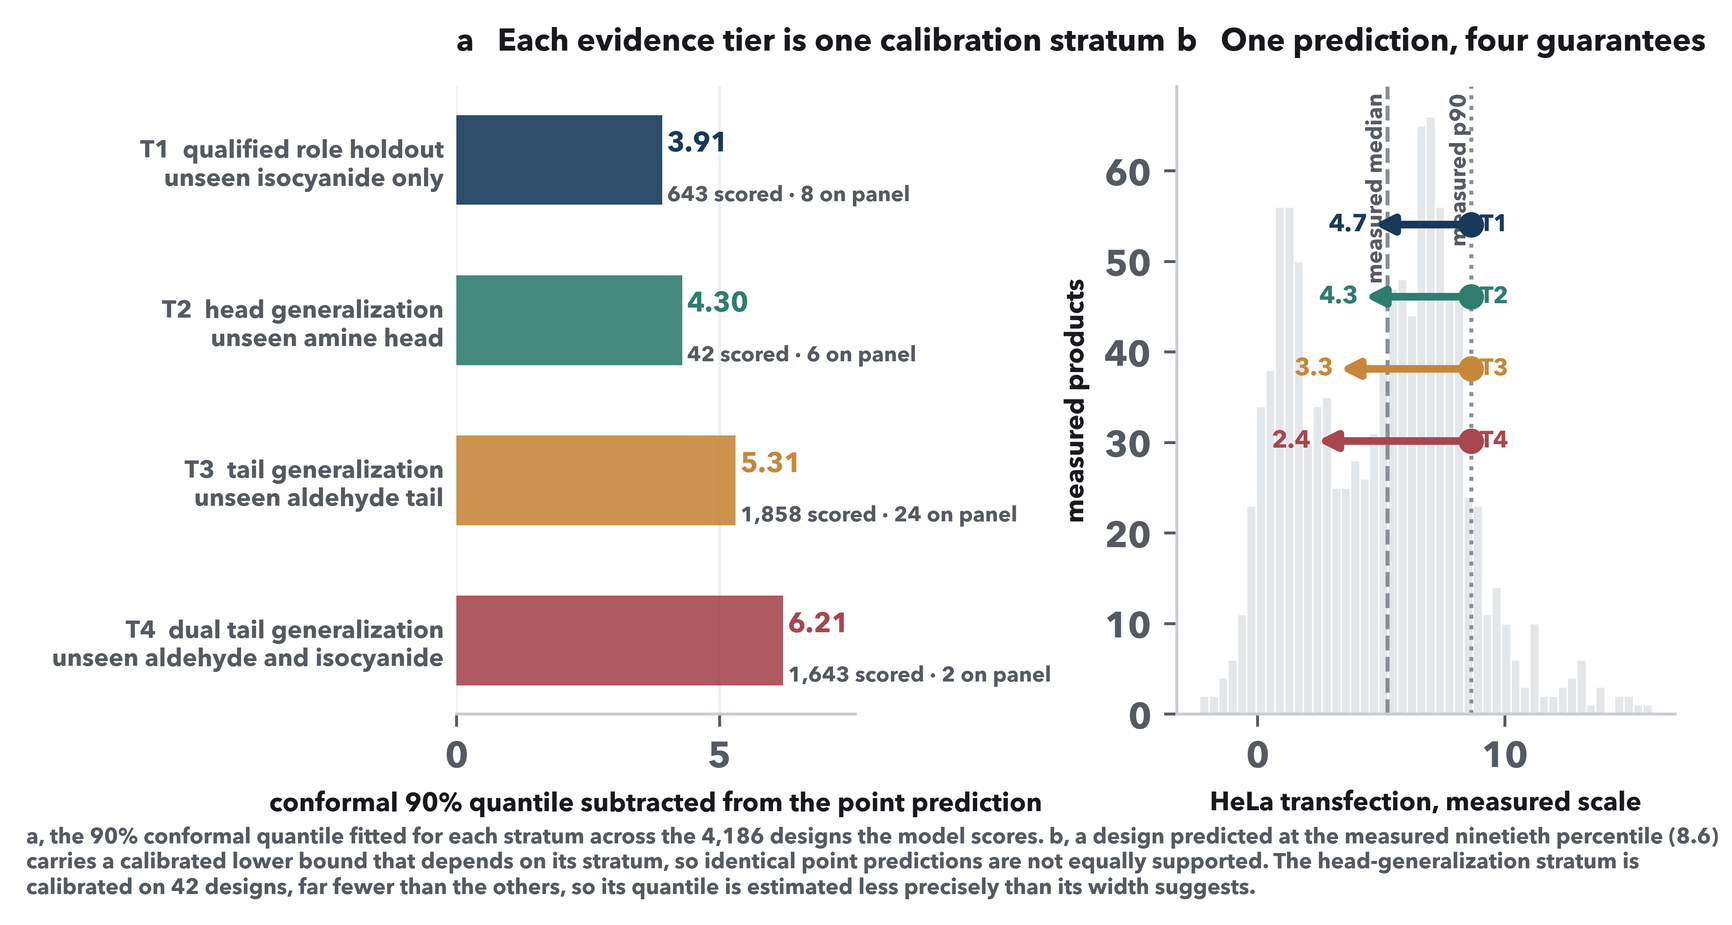
\includegraphics[width=0.92\textwidth]{panel_v6/calibration_by_tier.png}
\caption{\textbf{Conformal calibration by evidence tier, as used for the pilot.} Reproduced for
Library~0 only. The stratum quantile takes four discrete values across the pool, so within any one
stratum this ranking is identical to ranking by the point prediction, and the head-generalization
stratum rests on 42 calibration designs.}
\label{fig:calibration-tier}
\end{figure}

\begin{figure}[h]
\centering
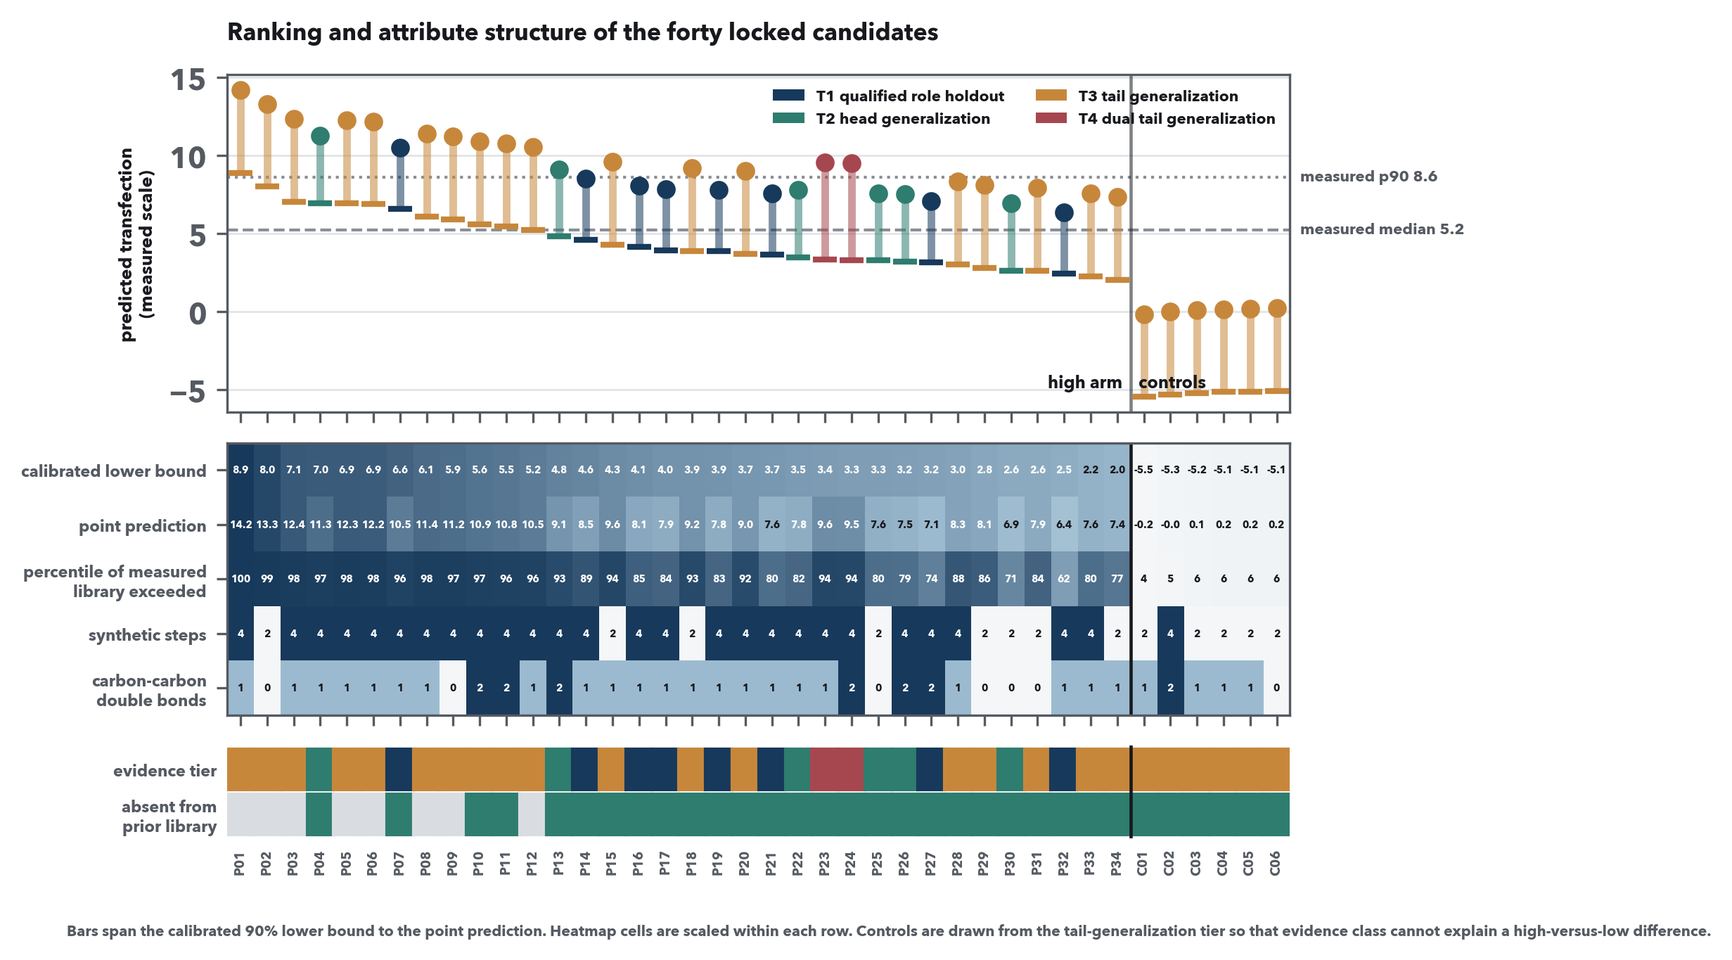
\includegraphics[width=0.92\textwidth]{panel_v6/panel_40_ranking_heatmap.png}
\caption{\textbf{The frozen ranking of the Library~0 pilot.} The ordering under the lower-bound
statistic. It does not define the prospective campaign.}
\label{fig:ranking-heatmap}
\end{figure}

The frozen pilot of \S\ref{app:library-zero} was ranked by a calibrated lower bound,
$\mathrm{lcb}_{90} = \hat{y} - q_{0.90}$, with $q_{0.90}$ a per-stratum conformal quantile. The
current formulation ranks on the ensemble mean. The difference is worth stating precisely, because
it is a change in where applicability sits rather than the correction of an error.

\paragraph{What the lower bound was doing.}
The stratum quantile takes only four values across the eligible pool, so within any one stratum
ranking by the lower bound is \emph{identical} to ranking by the point prediction
(Figure~\ref{fig:calibration-tier}). Its whole effect is between strata, where it penalises
membership in a weakly calibrated region. That is an applicability signal embedded in the score, and
it was chosen deliberately for that reason, not overlooked.

\paragraph{Where applicability sits instead.}
Applicability now enters as the admission predicate $E(G)$ of \S\ref{app:thresholds} rather than as a
penalty on the score. One statistic was doing two jobs, deciding both whether a molecule can be
ranked and where it ranks; separating them lets each be stated and checked on its own. The ranking
statistic differs between the two formulations because that second job moved.

\paragraph{Neither ranking can be shown superior.}
Re-running the frozen selector with only the sort key changed, and with eligibility, the
physicochemical envelope, route completeness, the Tanimoto ceiling, the head cap and both tie-breaks
held fixed, the two rules share \RankShared{} of 34 candidates and differ on \RankChanged{}. On axes
that neither statistic optimises the panels are close to equivalent: 13 against 14 distinct amine
heads, 22 against 24 aldehyde tails, and 26 against 25 candidates absent from the enumerated library.
Comparisons on median predicted potency or on the lower-bound floor are circular, each rule winning
on the quantity it sorts by, and no prospective measurement exists that could break the tie. We
therefore report the frozen panel under the rule it was selected with, and treat the alternative as a
sensitivity analysis rather than a correction.

\paragraph{What does not survive, and is not a matter of preference.}
The quantity must not be described as a validated 90\% bound. Its coverage was never established
prospectively, and for most of the panel the offset came from a fold carrying 20 calibration rows in
a scheme that missed its own coverage gate at 0.159 against a 0.100 maximum. Reporting it as a
calibrated interval would be a claim the calibration does not support, independently of which
statistic is used to rank.

% =============================================================================
\section{Semantic-Utility Analyses}
\label{app:semantics}
% =============================================================================

\subsection{Estimand and identifiability}
\label{app:estimand}
The estimand is the paired difference in denoising loss between two arms that are identical except
for the local role channel,
%
\[
\Dsem(t) = L_{\text{no-role}}(t) - L_{\text{true-role}}(t),
\]
%
reported per prediction head and aggregated over the six eligible heads. Positive values mean the
aligned arm reconstructs the clean state better.

The first version of this experiment was designed differently and was withdrawn, and the reason
determines the shape of the final design. That version sought to remove semantics entirely and
compare against a semantics-free generator. It is not identifiable. Role is recoverable from the
structural organization the model needs anyway: the per-role counts in $c$ determine where each role
block begins and ends, so an arm denied the explicit role tag still receives everything required to
derive role. Removing role information would mean removing $c$, and removing $c$ removes the design
problem rather than the semantics.

What is identifiable is narrower and, we think, more interesting: the value of presenting an
explicitly derivable quantity to a network of finite capacity, holding the global state and context
fixed. That is what \Dsem{} measures. Appendix~\ref{app:mi} sets out the consequence, which is that
\Dsem{} is not an information quantity and must not be reported as one.

\subsection{Matched experimental contract}
\label{app:parity}
\begin{table}[h]
\centering
\caption{Parity across the three arms. Only the local role channel differs.}
\label{tab:parity}
\small
\begin{tabular}{@{}lccc@{}}
\toprule
Quantity & no-role & true-role & misaligned \\
\midrule
Graph serialization & same & same & same \\
Parameter count & 1{,}150{,}892 & 1{,}150{,}892 & 1{,}150{,}892 \\
Initialization & paired & paired & paired \\
Minibatches & paired & paired & paired \\
Flow times $t$ & paired & paired & paired \\
Corruption draws & paired & paired & paired \\
Design program $c$ & same & same & same \\
Global position embedding & present & present & present \\
Local role channel & null tag & aligned & permuted \\
\bottomrule
\end{tabular}
\end{table}

% 1150892 is the pilot count (step 3000), not the production 1159916 - checked all 7 checkpoints
Two features of the contract deserve emphasis because they are what make the comparison a
comparison rather than a confound.

\emph{Capacity parity is exact, not approximate.} The no-role arm does not simply omit the role
embedding, which would leave it with fewer parameters and confound semantics with capacity. It
receives a constant null tag through the same embedding of the same dimension, so every arm has an
identical parameter count and an identical computation graph. The misaligned arm receives a permuted
role assignment matched in dimensionality and in label frequency.

\emph{The ablation removes experiment-specific semantics, never generic modelling capacity.} Every
arm retains a global position embedding sized to the maximum total atom count. An earlier version of
the specification would have denied the ablated arm any positional signal at all, which would have
crippled it and made the comparison meaningless; what is removed is the role-relative coordinate and
the role tag, not the ability to know where in the molecule a position sits.

Randomness is paired at every level that could otherwise dominate a paired difference:
initialization, minibatch composition, corruption draws and the flow-time grid are shared across arms
within a seed, so \Dsem{} is a within-seed contrast rather than a between-run one. Two invariants were
checked rather than assumed: that the flat and structured serializations induce the same graph up to
permutation, and that the design program is unchanged across arms.
All seven pilot checkpoints carry exactly 1{,}150{,}892 parameters at step 3000, which is the count reported above and is distinct from the production generator's 1{,}159{,}916.

\subsection{Main result}
\label{app:sem-main}
Across \SemSeeds{} paired seeds the aligned map reduces total denoising loss by
$\SemGapMag \pm \SemGapSD$, and the improvement is positive for all \SemHeads{} reported heads in
every seed. Sign consistency across every reported head and every seed is the load-bearing
observation here rather than the magnitude: with three seeds a mean difference alone would be weak
evidence, whereas eighteen of eighteen head-by-seed contrasts sharing a sign is not plausibly noise.
Table~\ref{tab:sem-per-head} gives every cell.

The effect is strongly corruption-dependent. Taking the ratio of \Dsem{} near the corrupted end of
the path to \Dsem{} near the clean endpoint gives \CorruptLow{}, 9.89 and \CorruptHigh{} across the
three seeds (Table~\ref{tab:sem-corruption}). We report the three values rather than a range because
the spread is itself informative: the direction is identical in every seed while the magnitude varies
by roughly 50\%, so the qualitative dependence replicates even though its size is not tightly
estimated at $n = 3$.

\paragraph{Two different six-head sets exist in this project; they are not interchangeable.}
This report's six are the semantic pilot's reported heads: the aggregate total together with atom
state, parent bond, offspring topology, closure bond and decoration anchor. All six improve in all
three seeds. A \emph{different} six is used by the role-divergence analysis of
\S\ref{app:negatives}, which drops the decoration anchor because its target is positional rather than
categorical and adds the decoration atom and decoration bond heads. Those two added heads are
\emph{not} uniformly positive: decoration atom is $-0.00219$ and decoration bond is $-0.05537$ in
seed s2, and decoration bond is marginally negative averaged over seeds. Any statement of the form
``all six heads'' must therefore name which six it means, and no result stated over one set may be
restated over the other.


\begin{table}[h]
\centering
\caption{The semantic-utility gap along the probability path, per paired seed. Low $t$ is the
strongly corrupted end. The gap falls monotonically toward the clean endpoint in every seed.}
\label{tab:sem-by-t}
\small
\begin{tabular}{@{}lrrrr@{}}
\toprule
$t$ & s1 & s2 & s3 & mean \\
\midrule
0.10 & $+0.5126$ & $+0.3206$ & $+0.4617$ & $+0.4316$ \\
0.25 & $+0.4449$ & $+0.2801$ & $+0.4138$ & $+0.3796$ \\
0.50 & $+0.2909$ & $+0.1827$ & $+0.2637$ & $+0.2458$ \\
0.75 & $+0.1630$ & $+0.1017$ & $+0.1427$ & $+0.1358$ \\
0.90 & $+0.0666$ & $+0.0324$ & $+0.0410$ & $+0.0467$ \\
\bottomrule
\end{tabular}
\end{table}

The dependence is monotone in all three seeds and spans roughly an order of magnitude between the
ends of the grid, which is the pattern \S\ref{app:mi} accounts for: as $t$ falls, the corrupted state
carries less about the molecule while the arithmetic the ablated arm must perform on $c$ is
unchanged, so explicit role becomes progressively more load-bearing.

\subsection{Misalignment control}
\label{app:misalign}
Misalignment recovers \MisalignRecovered{} of the aligned arm's benefit. The sign is negative: the
misaligned arm is not merely worse than the aligned arm, it is on aggregate slightly worse than
receiving no role at all, and it is worse than the no-role arm on \MisalignWorseHeads{} eligible
heads while being approximately tied on the remaining two.

That is the result the control was built to obtain. A channel matched in dimensionality and in label
frequency, differing only in whether the correspondence to chemistry is correct, produces none of the
gain. The benefit therefore cannot be attributed to the presence of an extra categorical input, to
added embedding parameters, or to the label distribution; it requires the correspondence itself.
Reading it alongside \S\ref{app:mi}: a wrong-but-well-formed semantic channel gives a finite network
something to fit that does not organize the molecular state, which is worse than leaving it to derive
the organization from $c$.

\subsection{Information-theoretic interpretation}
\label{app:mi}
Write $X$ for the clean categorical state, $Z_t$ for the corrupted state at flow time $t$, $C$ for
the design context, and $R$ for the per-position role assignment. Under log loss the Bayes-optimal
risk of a predictor given a conditioning set is the conditional entropy of $X$ given that set, so
for the two arms
%
\[
L^{*}_{\varnothing}(t) = H\!\left(X \mid Z_t, C\right),
\qquad
L^{*}_{R}(t) = H\!\left(X \mid Z_t, C, R\right),
\]
%
and therefore
%
\begin{equation}
\label{eq:mi}
L^{*}_{\varnothing}(t) - L^{*}_{R}(t)
= I\!\left(X ; R \mid Z_t, C\right).
\end{equation}
%
Equation~\eqref{eq:mi} is the identity that makes a role channel look like an information channel,
and it is why the first version of this experiment was designed as an information-removal ablation.
That design was abandoned, and the reason is worth stating plainly rather than leaving implicit.

\paragraph{Why the measured gap is not a mutual information.}
In FORGE the role map is a deterministic function of the design context: $c$ carries the per-role
atom counts, junction budgets, cycle ranks and attachment counts, and those counts fix which
serialized positions belong to which role. Hence $R$ is $\sigma(C)$-measurable, and the right-hand
side of Eq.~\eqref{eq:mi} is identically zero. At the Bayes optimum, with unbounded capacity, the
two arms would achieve the same risk and $\Dsem$ would vanish.

The gap we measure is nonetheless large and reproducible. It follows that $\Dsem$ does not estimate
an information quantity at all. It measures the \emph{computational} value of presenting a derivable
quantity explicitly to a capacity-limited network: the ablated arm must recover block boundaries
from the counts in $c$ by arithmetic over positions before it can use role at all, and at finite
width and depth it does not fully do so. We therefore report $\Dsem$ as an empirical
semantic-utility gap throughout, never as a conditional mutual information, and we make no claim
that it bounds one. No inequality direction is available in either sense, because neither arm attains
the Bayes optimum and the ablated arm's shortfall need not be smaller than the treated arm's.

The capacity at which the gap would close is not reachable in this setting, which is what makes the
limit a mathematical statement rather than a practical one. Capacity here is bounded by data and not
by compute: the corpus holds \CorpusSize{} products, and the pilot
resolves the gap at 1{,}150{,}892 parameters. Scaling toward the regime where the two arms converge
would overfit this corpus long before it reached it. The claim we make is correspondingly scoped, and
it is the one that matters for anyone working under comparable evidence: presenting role explicitly
is worth a measurable amount at every capacity this dataset supports.

This is also what forced the design of the third arm. Since role information cannot be removed from
$C$ without removing the structural program the model needs, a genuine control cannot be an
information-removal arm. The misaligned arm instead holds the channel, its dimensionality and its
label frequencies fixed while destroying the correspondence, which isolates explicit correct
alignment rather than channel presence. Appendix~\ref{app:parity} records the parity that makes the
three arms comparable.

\paragraph{Why utility grows as $t \to 0$.}
As $t \to 0$ the path in Eq.~\eqref{eq:path} approaches the role-specific source marginals, so $Z_t$
becomes progressively less informative about $X$ while the arithmetic the ablated arm must perform on
$c$ is unchanged. Two effects compound. The corrupted state supplies less positional disambiguation,
so role must carry more of the conditioning; and the role-specific source distributions $p_0^{h,r}$
differ across roles, so at small $t$ the correct role is precisely what identifies which marginal a
position was drawn from. Both make explicit role more load-bearing exactly where the molecular state
is least informative, which is the dependence reported in \S\ref{sec:res-semantics}.

\subsection{Predeclared hypotheses that were not supported}
\label{app:negatives}
% keep this titled as hypotheses not supported, not "additional analyses"
Three hypotheses were declared before the corresponding quantity was computed and were not
supported. All three are reported here because each constrains what the paper claims, and none is
re-tested under an alternative measure.

\paragraph{Semantic utility does not track role-wise marginal divergence.}
The natural mechanistic story is that role helps most where the roles differ most, so we declared a
measure in advance: the Jensen--Shannon divergence among the three role-conditional empirical target
distributions per head, uniform mixture reference, base-2 logarithms. The association with per-head
semantic utility is \emph{negative}, Spearman $\rho = -0.543$ over six heads. The power limitation was
also stated in advance and stands: with six points only a near-perfect ordering could reach
conventional significance, so this analysis is descriptive and secondary whatever it shows, and it is
not featured as a primary result. No alternative divergence measure was computed after seeing this
one. What it rules out is the simplest mechanistic account; it does not rule out the effect, which is
established by the paired design and the misalignment control rather than by this correlation.

\paragraph{Semantics do not act as a data-efficiency advantage.}
We declared that if role functions as an inductive bias, its benefit should be larger under sparser
supervision. Five of six heads moved in the wrong direction. The advantage is therefore not a
sample-efficiency effect in the sense that hypothesis proposed, and we make no data-efficiency claim.

\paragraph{Semantics do not confer held-family extrapolation.}
We declared strata of increasing structural distance from the training families and predicted that
semantic utility would grow with distance. The two most distant strata are negative, at $-0.10$ and
$-0.39$. We therefore make no claim that chemistry-informed semantics improve generalization to unseen
component families, and \S\ref{sec:res-semantics} confines itself to denoising ambiguity under
corruption, which is what the evidence supports.

Reported together these bound the claim tightly. The effect is real, replicated, and not explained by
channel presence or label frequency; and it is not a data-efficiency effect, not an extrapolation
effect, and not predicted by how much the role-conditional distributions differ.
\begin{table}[h]
\centering
\caption{Role differentiation against semantic utility, ordered by divergence. If the simple
mechanistic account held, these columns would rise together. They do not.}
\label{tab:divergence}
\small
\begin{tabular}{@{}lrrr@{}}
\toprule
Head & JSD (bits) & mean $\Dsem$ & $\Dsem$ at $t=0.10$ \\
\midrule
decoration bond  & 0.6638 & $-0.00047$ & $-0.00463$ \\
closure bond     & 0.2180 & $+0.01713$ & $+0.06127$ \\
decoration atom  & 0.2081 & $+0.00280$ & $+0.00143$ \\
atom state       & 0.1510 & $+0.02656$ & $+0.04720$ \\
offspring        & 0.0953 & $+0.14092$ & $+0.20645$ \\
parent bond      & 0.0818 & $+0.01703$ & $+0.03236$ \\
\bottomrule
\end{tabular}
\end{table}

Spearman $\rho = -0.543$ with a two-sided permutation $p = 0.297$ over $10^5$ label permutations for
the seed-averaged gap, and $\rho = -0.429$ with $p = 0.420$ at $t = 0.10$. The ordering is close to
inverted: the head with the largest role differentiation, decoration bond at 0.664 bits, has the only
negative mean gap, while offspring topology has the smallest divergence at 0.095 bits and much the
largest benefit.

% =============================================================================
\section{Lipid-Native Molecular Evaluation}
\label{app:lipid_metrics}
% =============================================================================

\subsection{Why these descriptors}
\label{app:why-descriptors}
The panel was assembled to cover the axes along which ionizable-lipid design is known to vary, not
to maximize the difference between FORGE and its baselines. That distinction is procedural rather than
rhetorical, and it was enforced by a prior commitment.

An earlier version of this analysis proposed selecting the main-text metrics as ``the ones the panel
already discriminates on''. That is post-hoc metric selection: with \PanelSize{} descriptors and a
free choice of which to feature, a difference can be manufactured from noise. The commitment adopted
in response fixes the \MainMetricCount{} main-text metrics by \emph{scientific coverage} rather than
by observed effect size, one per design axis, chosen before the per-descriptor comparison was read.
Every remaining descriptor is reported here regardless of what it shows, which is the other half of
the same commitment: a panel is only a guard against cherry-picking if the unselected members are
also published.

\subsection{Descriptor dictionary}
\label{app:descriptor-dict}
\begingroup\small
\begin{longtable}{@{}p{4.0cm}p{2.6cm}p{6.2cm}@{}}
\caption{The complete lipid-native descriptor panel. Counts are over the region named in the second column; SMARTS patterns are given where a descriptor is a substructure match.}\label{tab:descriptor-dict}\\
\toprule
Descriptor & Region & Definition \\
\midrule
\endfirsthead
\toprule Descriptor & Region & Definition \\ \midrule \endhead
\bottomrule
\endfoot
\texttt{ald\_alkenes} & aldehyde tail & SMARTS \texttt{[CX3]=[CX3]} \\
\texttt{ald\_branches} & aldehyde tail & SMARTS \texttt{[CX4;\$(C(-[\#6])(-[\#6])-[\#6])]} \\
\texttt{ald\_carbons} & aldehyde tail & carbon count \\
\texttt{ald\_esters} & aldehyde tail & SMARTS \texttt{[CX3](=[OX1])[OX2][CX4]} \\
\texttt{ald\_ethers} & aldehyde tail & SMARTS \texttt{[CX4][OX2][CX4]} \\
\texttt{ald\_heavy\_atoms} & aldehyde tail & heavy-atom count \\
\texttt{ald\_ketones} & aldehyde tail & SMARTS \texttt{[CX4][CX3](=[OX1])[CX4]} \\
\texttt{ald\_longest\_chain} & aldehyde tail & longest contiguous carbon chain \\
\texttt{clogp} & whole lipid & Crippen logP \\
\texttt{degradable\_linkages} & whole lipid & ald\_esters $+$ iso\_esters \\
\texttt{hba} & whole lipid & H-bond acceptors \\
\texttt{hbd} & whole lipid & H-bond donors \\
\texttt{head\_hba} & ionizable head & H-bond acceptors \\
\texttt{head\_hbd} & ionizable head & H-bond donors \\
\texttt{head\_heavy\_atoms} & ionizable head & heavy-atom count \\
\texttt{head\_max\_n\_spacing} & ionizable head & largest topological distance between two head nitrogens \\
\texttt{head\_min\_n\_spacing} & ionizable head & smallest topological distance between two head nitrogens \\
\texttt{head\_nitrogens} & ionizable head & nitrogen count \\
\texttt{head\_primary\_amine} & ionizable head & SMARTS \texttt{[NX3;H2;!\$(NC=O)]} \\
\texttt{head\_ring\_nitrogen} & ionizable head & SMARTS \texttt{[nX2,NX3;R]} \\
\texttt{head\_rings} & ionizable head & ring count \\
\texttt{head\_secondary\_amine} & ionizable head & SMARTS \texttt{[NX3;H1;!\$(NC=O)]} \\
\texttt{head\_tertiary\_amine} & ionizable head & SMARTS \texttt{[NX3;H0;!\$(NC=O);!\$(N=*)]} \\
\texttt{head\_to\_tail\_ratio} & ionizable head & head\_heavy\_atoms / total\_tail\_carbons \\
\texttt{iso\_alkenes} & isocyanide tail & SMARTS \texttt{[CX3]=[CX3]} \\
\texttt{iso\_branches} & isocyanide tail & SMARTS \texttt{[CX4;\$(C(-[\#6])(-[\#6])-[\#6])]} \\
\texttt{iso\_carbons} & isocyanide tail & carbon count \\
\texttt{iso\_esters} & isocyanide tail & SMARTS \texttt{[CX3](=[OX1])[OX2][CX4]} \\
\texttt{iso\_ethers} & isocyanide tail & SMARTS \texttt{[CX4][OX2][CX4]} \\
\texttt{iso\_heavy\_atoms} & isocyanide tail & heavy-atom count \\
\texttt{iso\_ketones} & isocyanide tail & SMARTS \texttt{[CX4][CX3](=[OX1])[CX4]} \\
\texttt{iso\_longest\_chain} & isocyanide tail & longest contiguous carbon chain \\
\texttt{molecular\_weight} & whole lipid & molecular weight \\
\texttt{rotatable\_bonds} & whole lipid & rotatable bonds \\
\texttt{tail\_asymmetry} & whole lipid & $|\,$ald\_carbons $-$ iso\_carbons$\,|$ \\
\texttt{tail\_balance} & whole lipid & ald\_carbons / total\_tail\_carbons \\
\texttt{total\_tail\_carbons} & whole lipid & ald\_carbons $+$ iso\_carbons \\
\texttt{tpsa} & whole lipid & topological polar surface area \\
\end{longtable}
\endgroup

Counts are integers over the named region; \texttt{tail\_balance} and
\texttt{head\_to\_tail\_ratio} are dimensionless ratios, and \texttt{clogp}, \texttt{tpsa} and
\texttt{molecular\_weight} carry their usual units. The three regional prefixes follow the Ugi
decomposition, so a descriptor prefixed \texttt{head\_} is computed on the amine-derived component
graph rather than on the whole lipid, which is what allows head chemistry and tail chemistry to be
compared separately in \S\ref{app:panel-results}.

\subsection{Full results}
\label{app:panel-results}
The comparison is three-way: held-out real lipids, FORGE samples, and the role-marginal null. The
null is the informative comparator rather than a straw man, because it shares FORGE's declared
support, masks, role-specific empirical marginals and admission procedure, and differs only in having
no contextual denoiser. Any descriptor on which the null already matches the real lipids is a
descriptor explained by one-variable statistics plus chemistry constraints, and FORGE deserves no
credit for it.

Two results anchor the reading. The null reaches full chemical admission while building the
prespecified ionizable-head architecture in \NullHeadRate{} of \NullDraws{} samples, so declared
support plus marginals is demonstrably not sufficient for lipid-native head chemistry. And FORGE
overshoots rather than matching: \WantedHeadForge{} against \WantedHeadReal{} in the real set, a
roughly 22\% overshoot. We report the overshoot as an overshoot. A model that built the architecture
more often than real lipids do has not reproduced the target distribution, and the grouped classifier
of \S\ref{app:grouped-auc} says the same thing in aggregate.
Table~\ref{tab:panel-full} in \S\ref{app:panel-tables} reports all \PanelSize{} descriptors.

\subsection{Grouped real-versus-generated classifier}
\label{app:grouped-auc}
A classifier trained to separate generated from held-out real lipids reaches AUC \GroupedAUC{}.
Grouping is what makes this number meaningful: products sharing a component are not independent
observations, so the split is grouped rather than random, and the reported AUC is aggregated across
groups rather than pooled over products.

We interpret \GroupedAUC{} as \emph{residual separability} and nothing stronger. It is well above
chance, so FORGE has not matched the real distribution and we make no distribution-matching claim; it
is also well below one, so the generated designs are not trivially separable either. Read together
with the per-descriptor panel, the picture is a model that has acquired lipid-native organization in
the specific respects the panel names while remaining distinguishable in aggregate.
Table~\ref{tab:grouped-auc} gives the per-fold values and the grouping unit.
The classifier is a histogram gradient-boosted tree with 200 iterations at a fixed seed, taking the full \PanelSize{}-descriptor vector as its feature set, so it sees exactly the panel and no additional structural information. Folds are \texttt{GroupKFold} over the grouping unit, and the reported figure is the mean of the per-fold areas rather than a pooled curve.

\subsection{Ester-linkage decomposition}
\label{app:ester}
Ester-linked tail chemistry is the clearest case of a miss that was diagnosed rather than absorbed.
Early configurations produced ester linkages in 0.029 of admitted designs against a training-fold
prevalence of \EsterTrainFold{}, a nearly twenty-fold shortfall on the single most characteristic
linker motif in the corpus.

The shortfall decomposed into two separable causes. Changing the architecture moved the rate from
0.029 to 0.190. Changing the training budget moved it from 0.190 to \EsterForge{}, against the
\EsterTrainFold{} training prevalence. Each stage changed one factor, and the stages must be read
that way: this is not an architecture-only causal progression, and the second step is a
budget effect that would have been misattributed to representation had both been changed together. The
ester-enriched held-family reference sits at \EsterMatchedRef{}, which is the relevant comparator for
a matched-family evaluation rather than the train-fold prevalence.

% =============================================================================
\section{Reproducibility, Configurations, and Artifact Registry}
\label{app:reproducibility}
% =============================================================================

\subsection{Where the claim-to-evidence index lives}
\label{app:claim-index}
The claim-to-evidence index is the Evidence Map at the head of this appendix rather than a table
here, so that a reviewer meets it before the technical material rather than after it.

\subsection{Artifact registry}
\label{app:registry}
Every reported quantity traces to a frozen artifact carrying its own SHA-256, and every artifact
records the configuration, input hashes, seeds and runtime that produced it. Rather than reproduce
those strings in prose, where they are unreadable and cannot be checked, this section states the
conventions and points at the artifacts; the Evidence Map at the head of this appendix maps each
main-text claim to its source.

Four conventions govern how the artifacts should be read.

\emph{Numbers are single-sourced.} Every quantity in the main text and in this appendix is a macro
resolved from one ledger entry, never retyped at the point of use. Tables S1--S16 are emitted by a
generator directly from artifacts and are marked do-not-edit-by-hand; Table S17 is generated the same
way. A number that appears twice in this document appears twice because one macro was used twice.

\emph{Checkpoints are named, not assumed.} The production refit at 5,100 steps and the step-3000
pilot checkpoints back disjoint sets of claims, per \S\ref{app:optim}.

\emph{Seeds are recorded per analysis rather than globally.} Bootstrap, permutation and blinding seeds
differ across analyses and are stored with the artifact that used them, because a single global seed
would make independent analyses spuriously correlated.

\emph{Software is pinned to the artifact, not the environment.} The reported version is the one that
produced the frozen artifacts, which is not necessarily the one currently installed; see
\S\ref{app:corpora}.
\begin{table}[h]
\centering
\scriptsize
\caption{Artifact registry. Every reported quantity traces to one frozen artifact; each artifact records its own configuration, input hashes, seeds and runtime.}
\label{tab:registry}
\begin{tabular}{@{}p{4.0cm}p{6.1cm}p{2.4cm}@{}}
\toprule
Claim & Artifact & Checkpoint \\
\midrule
semantic-utility gap, total head & \texttt{results/phase1/forge\_semantics\_pilot\_v1/closure.json} & flat\_no\_role / flat\_true\_role step 3000 \\
corruption amplification, t=0.10 over t=0.90 & \texttt{results/phase1/forge\_semantics\_pilot\_v1/closure.json} & step 3000 \\
misaligned control, total head & \texttt{results/phase1/forge\_semantics\_pilot\_v1/closure.json} & step 3000 \\
role-divergence association (Amendment 14) & \texttt{results/phase1/forge\_role\_divergence\_association\_v1/result.json} & n/a, no training \\
wanted head architecture (1 handle + tertiary ionizable N) & \texttt{results/phase1/forge\_held\_family\_stage2\_v1/amphiphile\_panel\_v3.json} & ugi\_decoration\_coupling\_v1/challenger/checkpoint\_step\_3000.pt \\
two or more Ugi-reactive sites & \texttt{results/phase1/forge\_held\_family\_stage2\_v1/amphiphile\_panel\_v3.json} & ugi\_decoration\_coupling\_v1/challenger/checkpoint\_step\_3000.pt \\
ester-linked aldehyde tail & \texttt{results/phase1/forge\_held\_family\_stage2\_v1/amphiphile\_panel\_v3.json} & ugi\_decoration\_coupling\_v1/challenger/checkpoint\_step\_3000.pt \\
grouped two-sample AUC against real lipids & \texttt{results/phase1/forge\_held\_family\_stage2\_v1/amphiphile\_panel\_v3.json} & challenger step 3000 \\
role-marginal null builds an ionizable head & \texttt{results/phase1/forge\_held\_family\_stage2\_v1/null\_marginal\_null.json} & null denoiser, no trained weights \\
absent from the production training corpus & \texttt{results/phase1/ugi\_novelty\_audit\_v1/result.json} & decoration-coupling production refit \\
outside the finite enumeration & \texttt{docs/FORGE\_PENDING\_MANUSCRIPT\_CHANGES.md 3g; tests/test\_enumeration\_membership\_convention.py pins the convention} & production refit \\
distinct aldehyde components generated & \texttt{results/phase1/ugi\_novelty\_audit\_v1/result.json} & production refit \\
distinct amine head components generated & \texttt{results/phase1/ugi\_novelty\_audit\_v1/result.json} & production refit \\
distinct isocyanide components generated & \texttt{results/phase1/ugi\_novelty\_audit\_v1/result.json} & production refit \\
route-complete out-of-enumeration designs & \texttt{results/phase1/forge\_open\_world\_actionability\_funnel\_v1/result.json} & production refit \\
fresh prediction-supported yield & \texttt{results/phase1/ugi\_morphology\_proposal\_challenger\_adjudication\_v1/result.json} & production refit \\
exploration cost of enrichment & \texttt{results/phase1/ugi\_morphology\_proposal\_challenger\_adjudication\_v1/result.json} & production refit \\
pooled descriptive calibration coverage & \texttt{results/phase1/ugi\_interpolative\_conformal\_v1/result.json} & frozen predictive ensemble \\
unique forward assembly, all admitted & \texttt{results/phase1/forge\_forward\_outcome\_census\_v1/result.json} & production refit \\
unique forward assembly, prediction-supported & \texttt{results/phase1/forge\_forward\_outcome\_census\_v1/result.json} & production refit \\
unique forward assembly, frozen 40 / Library 0 & \texttt{results/phase1/forge\_forward\_outcome\_census\_v1/result.json} & production refit \\
route completeness by enumeration membership & \texttt{results/phase1/forge\_open\_world\_actionability\_funnel\_v1/result.json} & production refit \\
designs resolving to purchasable starting material, pooled & \texttt{results/phase1/forge\_open\_world\_actionability\_funnel\_v1/result.json} & production refit \\
single-step route recovery, top 5 & \texttt{results/phase1/graph2edits\_single\_step\_recovery\_benchmark\_v1/score.json} & n/a, external engines \\
bounded hybrid route cascade on the 256-product shortlist & \texttt{results/phase1/ugi\_bounded\_hybrid\_route\_cascade\_v1/result.json} & production refit \\
Library 0 status & \texttt{results/phase1/ugi\_prospective\_panel\_v6/prospective\_panel.jsonl.gz} & production refit \\
\bottomrule
\end{tabular}
\end{table}

Table~\ref{tab:registry} lists the 26 ledger entries with their artifacts. SHA-256 values, input
hashes and per-analysis seeds are recorded inside each artifact rather than reproduced here, where
they would be unreadable and unverifiable. Three ancillary diagnostic artifacts, covering
distribution overlap, route-saturation sampling and an early semantic-annotation probe, were produced
under a later RDKit release than the one reported in \S\ref{app:corpora}; none of them backs a number
reported in this paper.
Each artifact additionally records its own runtime block: elapsed seconds, platform string, Python version and, where a model was trained or evaluated, the PyTorch version. Structural analyses ran on macOS arm64 under Python 3.14.2 with PyTorch 2.11.0; generator training and the semantic pilot ran in deterministic float32 on a single NVIDIA L4, per Table S16. Because the runtime block travels inside each artifact rather than being asserted centrally, a reader checking one number does not have to trust a global claim about the environment.

\subsection{Analyses not performed and claims not made}
\label{app:nonclaims}
The following are \emph{not} claimed anywhere in this paper. Each is listed because the surrounding
material could otherwise be read as implying it.

\begin{itemize}\tightlist
\item \textbf{No cross-reaction generalization.} The formulation is stated for modular families
  generally; every experiment uses Ugi-3CR. No model was trained or evaluated on a second chemistry.
\item \textbf{No stereochemical generation.} Generation is constitutional. FORGE proposes no
  stereocentres and makes no claim about stereochemical preference, which is a known determinant of
  LNP behaviour \citep{hatit2023nanoparticle}.
\item \textbf{No predictive coverage guarantee.} Calibration is descriptive. No conformal or other
  finite-sample coverage claim is made for any candidate, inside or outside \Spred{}.
\item \textbf{No distribution matching.} A grouped classifier separates generated from real lipids at
  AUC \GroupedAUC{}, and the model overshoots the real ionizable-head rate.
\item \textbf{No semantic data-efficiency advantage} and \textbf{no semantic held-family
  generalization}, both predeclared and both unsupported; see \S\ref{app:negatives}.
\item \textbf{No mechanistic LNP model.} Nothing here models particle packing, apparent pK$_\text{a}$,
  endosomal escape, or any physical mechanism linking structure to delivery.
\item \textbf{No synthesis, formulation or biological result.} No member of any panel has been made.
  Every prospective quantity is a marked placeholder.
\item \textbf{No route proposal treated as evidence}, and \textbf{no unresolved chemistry called
  unsynthesizable}; see \S\ref{app:tooling}.
\item \textbf{No claim that either ranking statistic is superior.} The two cannot be ordered
  without prospective outcomes; see \S\ref{app:lcb-ranking}.
\item \textbf{No comparison against external generative models.} This is a scope choice rather than
  an omission. The claim under test is that known chemistry can organize open-ended generation for a
  molecular family, and the quantity that would distinguish methods, composition of precursor
  chemistry outside a fixed inventory, is identically zero for inventory-constrained systems. A
  comparison would therefore measure a definitional difference rather than a performance one. The
  evidence here is internal: the semantic ablation with its misaligned control, and the role-marginal
  null. See \S\ref{sec:res-fidelity}.
\item \textbf{The declared support is not itself ablated.} Section~\ref{sec:support} and
  Proposition~\ref{prop:sampler} state that the support constrains sampling, but no arm removes it:
  the role-marginal null operates \emph{inside} the same support and so cannot measure its
  contribution. What the support does for sample quality, as opposed to what it guarantees, is
  therefore unmeasured here.
\end{itemize}

\subsection{Completion checklist}
\label{app:checklist}

What remains open before submission falls into three kinds, and they are not equally tractable.

\emph{Values only the campaign can supply.} The candidate-lock date and hash, the procurement
snapshot refresh, the identity and affiliation of the reviewing chemist, which candidates were
selected for synthesis, and every prospective outcome.

\emph{Values recoverable from the record.} The tie-breaking rule applied by the current ranking, and
the comparator-predictor hyperparameters.

\emph{One thing that is not a missing value but a missing experiment.} An earlier plan specified
matched-budget comparisons against other generative models. Those runs do not exist, and the
placeholders that stood in for them in a previous draft should not be read as work awaiting
write-up. The controls reported here, the semantic ablation and the role-marginal null, answer a
different question, and \S\ref{app:nonclaims} states the absence rather than implying coverage.

Two numbers also carry a weaker provenance than the rest and are flagged where they appear: the
predictor's $R^2$ values of 0.504 in calibration and 0.253 in post-selection test are quoted from
the development record rather than resolved from a ledger entry, and should be re-derived or pinned
before submission.

% =============================================================================
\section{Synthesis Qualification and Actionability}
\label{app:synthesis}
% =============================================================================

\subsection{Admission is not synthesis}
\label{app:admission-ladder}
Four properties are distinct and are routinely conflated. \emph{Structural admission} says the
generated graph is chemically well formed and reassembles from its projected components.
\emph{Unique assembly} says those components produce that product and no other under the qualified
forward transform. \emph{Route completeness} says every component is purchasable or reducible to
purchasable material by a documented preparation. \emph{Successful synthesis} says someone made it.

Each is necessary for the next and none implies it. A design can be admitted and not uniquely
assembling, uniquely assembling and not route-complete, and route-complete and still fail at the
bench. The whole of this appendix is organized by that ladder, and no result in it should be read as
evidence about a rung above the one it measures.

\subsection{The admission operator}
\label{app:admission}
Admission is Eq.~\eqref{eq:admit}: the projected components must satisfy their role-specific
interfaces, and the qualified forward transform applied to them must reproduce the generated
constitutional graph up to isomorphism. Failures are rejected rather than repaired, and no sample is
resampled toward a target after failing.

Forward enumeration is capped at 100 products per component assignment. The cap was never reached:
the frozen census records \texttt{enumeration\_cap} 100 with
\texttt{designs\_hitting\_enumeration\_cap} 0, so uniqueness is decided by exhaustive enumeration
rather than truncated search for every design in the population. The value 128 appears elsewhere in
the route code for a different parameter and does not apply here.

\subsection{Unique forward assembly}
\label{app:unique}
Uniqueness asks whether the target is the \emph{only} distinct product enumerable from its own
components. Across admitted designs the rate is \UniqueAdmitted{}; among evidence-supported designs it
is \UniqueSupported{}. Within the frozen Library~0 pilot it is \LibraryZeroUnique{} of
\LibraryZeroN{}.

The mechanism behind non-uniqueness is fully determined and worth stating because it is narrower than
one might guess. Every non-unique design carries at least two reactive amine sites, and no other cause
was identified: with two such sites the Ugi condensation can proceed at either, giving a second
constitutional product from the same three components. An earlier reading attributed part of the
effect to competing ketone chemistry; that reading was withdrawn once the rate was compared against
its base rate in the population. Admission verifies that the target is produced; uniqueness verifies
that it is produced alone. These are different properties and the gap between them is chemistry, not
model error.

\subsection{Component realization}
\label{app:components}
Routing runs after generation and after the exact forward check, and never modifies a design. Its
pseudocode is Table S13; the per-candidate assignments are Table S11, the per-component records with
supplier counts are Table S10, and the consolidated purchase list is Table S12.

The three roles are asymmetric by design. \emph{Amine heads} carry no disconnection rule in this
instantiation, so an unseen head must be purchasable outright. \emph{Ester-linked aldehyde tails}
disconnect by esterification of a carboxylic acid with an $\alpha,\omega$-diol followed by oxidation
of the remaining primary alcohol, two steps, resolved only if both starting materials have supplier
records. \emph{Isocyanide tails} disconnect to the corresponding primary amine by formylation and
dehydration, two steps, resolved only if the amine has a supplier record. Both tail routes are
published chemistry applied to generated structures, not model proposals. Admission additionally
requires total steps at most four, counting across components and excluding the final Ugi assembly,
which is common to every design.

For the frozen pilot this resolves to 49 distinct catalogue materials, with 53 components purchased
directly and 67 prepared by a forward-verified route; 13 candidates require two synthetic steps and 27
require four. Figure~\ref{fig:route-tree} shows one design's full resolution. Every branch terminates
in a catalogue material, with no unresolved branch. Supplier records are dated snapshots and are not
guarantees of stock, purity or lead time.

\subsection{Route completeness outside the finite chemistry}
\label{app:routes}
\begin{figure}[h]
\centering
% width only here, setting height too squashes it (native 3900x2730)
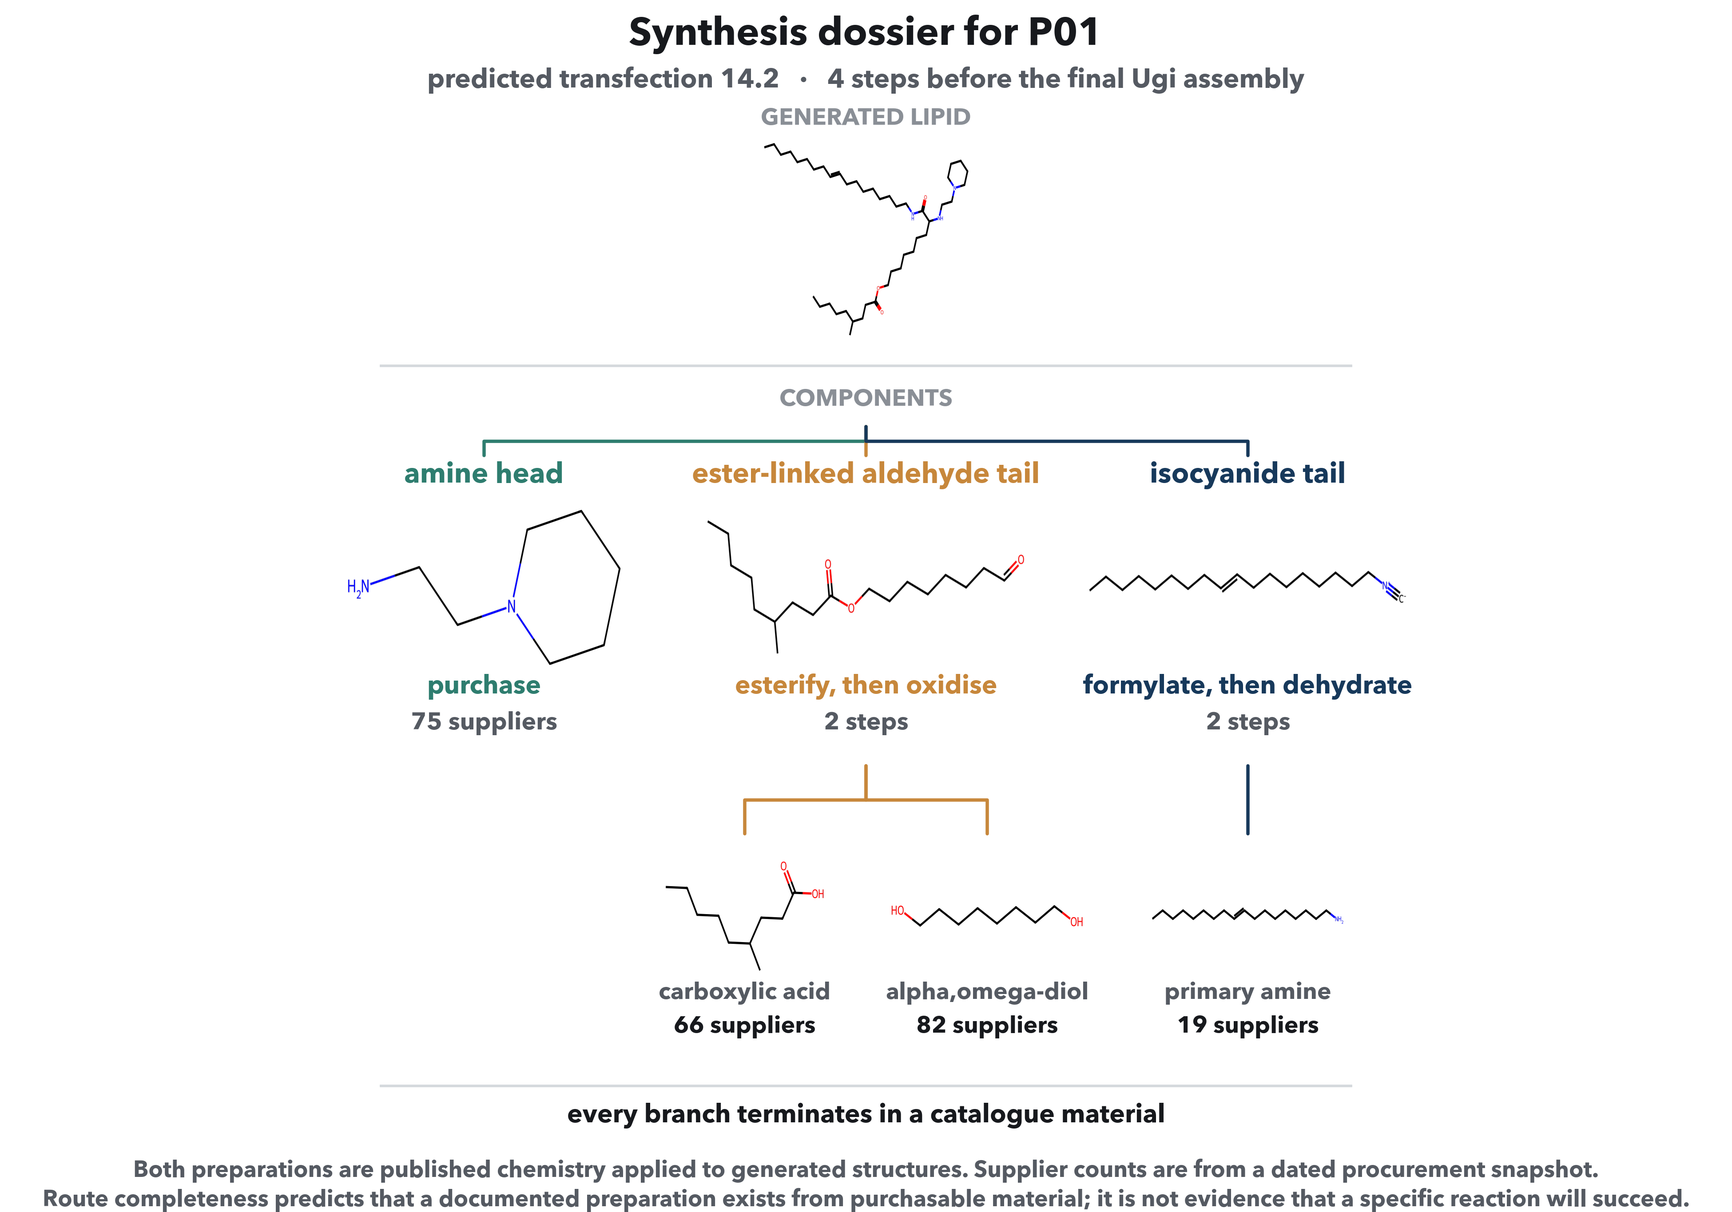
\includegraphics[width=\textwidth]{panel_v6/route_tree.png}
\caption{\textbf{Component routing for a single generated design.} The generated lipid is
projected to its three components; the amine head terminates directly in catalogue material, while
both tails are reduced to purchasable starting materials by published preparations. Supplier counts
come from a dated procurement snapshot. The predicted transfection value shown in the header is
provenance from the lower-bound ranking rule of \S\ref{app:library-zero} and is not a current
ranking quantity.}
\label{fig:route-tree}
\end{figure}

Route completeness is \RouteInside{} inside the enumerated reference chemistry, 541 of 541, against
\RouteOutside{} outside it, 931 of 1,008. The difference is \RouteDiff{} with a 95\% interval of
\RouteDiffCI{}, over 1,549 designs reaching route assessment.

The interval is a cluster bootstrap over \RouteClusters{} aldehyde components, not a product-level
i.i.d.\ bootstrap. That choice is substantive rather than conservative bookkeeping: products sharing
an aldehyde are not independent evidence about whether that aldehyde can be prepared, since a single
successful disconnection resolves every design using it. Resampling products independently would
count one preparation many times and shrink the interval to something the data do not support.

Two limits bound the claim. Route completeness is \emph{conditional on reaching route assessment}, so
designs removed earlier in the funnel have unmeasured route completeness and the outside-enumeration
figure is not a marginal rate over all generated chemistry. And route completeness is computational:
it predicts that a documented disconnection exists with purchasable starting materials, and it is not
evidence that any specific reaction will succeed at scale, in yield or in purity. The measured gap is
the honest form of the cost of leaving the finite library. It is a real cost, not parity, and the
interval marginally clears the prespecified $\pm 10$ point band.

\subsection{Where the off-registry chemistry sits, and which gate removes it}
\label{app:role-novelty}
The headline novelty figure counts designs carrying at least one component outside the
\RegistrySize{}-component training registry. That phrasing hides the role, and the roles are not
interchangeable: the amine head drives activity, and \S\ref{app:components} gives it no
disconnection rule, so an unseen head has to be purchasable outright. If novelty concentrated in the
tails, which are a homologous series where an unseen component often means a different chain length,
the reach would be worth much less than the number suggests.

Table~\ref{tab:role-novelty} splits the funnel by role. Two things follow. Novelty is heaviest on the
amine head at generation, not on the tails. And route assessment is not the filter: off-registry
components that reach it resolve at rates close to their on-registry counterparts for both the amine
head and the aldehyde tail. The isocyanide tail is the weakest role at \ResolveOffIso{}, which is the
opposite of what the disconnection asymmetry predicts.

The filter is the prediction-support gate. Designs with an unseen amine head are \OffAmineAdm{} of
admitted and \OffAmineSup{} of prediction-supported, a collapse of roughly two orders of magnitude in
one step, while unseen aldehyde tails survive and are enriched. This is the intended behavior of
\S\ref{sec:support}, not a defect: the activity model refuses to score head chemistry it has no
evidence for, and the head is exactly where it has least. It does mean the actionable set is confined
to catalogue heads by the predictor rather than by the chemistry, and that the way to widen it is
prospective measurement on new heads rather than a head disconnection rule.

Two cautions. The off-registry amine cell at route assessment holds ten designs, so
\ResolveOffAmine{} is an observation and not a rate worth an interval. And all resolution figures are
conditional on reaching assessment, so designs removed by earlier gates have unmeasured route status.

\begin{table}[h]
\centering
\caption{\textbf{Off-registry share by role through the funnel, and resolution at route assessment.}
Population is the union of both rescoring ledgers, \FunnelAdmitted{} distinct admitted products; the
abstract's pooled figure is over the main ledger alone and is not comparable row for row. Resolution
uses the accessibility standard of \S\ref{app:components}, purchasable or reducible to purchasable
material under a forward-verified disconnection within the step budget, not adjudicated closure.}
\label{tab:role-novelty}
\small
\begin{tabular}{@{}lrrrr@{}}
\toprule
& \multicolumn{3}{c}{off-registry share of designs} & \\
\cmidrule(lr){2-4}
Stage & amine head & aldehyde tail & isocyanide tail & $n$ \\
\midrule
Admitted                  & 49.7\% & 43.3\% & 15.2\% & \FunnelAdmitted{} \\
Prediction-supported      &  0.5\% & 31.4\% &  3.4\% & \FunnelSupported{} \\
Absent from train fold    &  0.7\% & 51.2\% &  5.6\% & 1{,}612 \\
Reaching route assessment &  0.6\% & 51.6\% &  5.8\% & \ResolveDen{} \\
\midrule
\multicolumn{5}{@{}l}{\emph{Resolution at route assessment}} \\
On-registry components    & 1{,}539/1{,}539 & 749/749 & 1{,}459/1{,}459 & \\
Off-registry components   & \ResolveOffAmine{} & \ResolveOffAld{} & \ResolveOffIso{} & \\
\bottomrule
\end{tabular}
\end{table}

Resolution also degrades with how much novelty a single design carries, which the per-role view
hides: designs with no off-registry component resolve at 664/664, with one at 802/870, and with two
at 6/15. Nothing in the assessed population carries three.

\subsection{Tooling}
\label{app:tooling}
\paragraph{Route levels.}
Resolution is organized into three levels. \textbf{L1} is exact Ugi decomposition and forward
reassembly of the product itself. \textbf{L2} is synthesis of each generated amine, aldehyde and
isocyanide component, or a declared direct commercial path for it. \textbf{L3} is closure of every
route leaf to a terminal material under the declared procurement and evidence snapshot. Routing is
post hoc to graph generation but \emph{not} post hoc to panel selection: the cascade is applied
identically to an arm-balanced, route-blinded shortlist before any panel is locked, so route attrition
is part of the reported outcome rather than an invisible cleanup step.

\paragraph{The resolution hierarchy.}
Within L2 the order is fixed and each stage is consulted only where the previous one is silent.
Exact evidence comes first: a frozen curated index of qualified component routes terminating in a
current terminal-material ledger. Where the index is silent, \textbf{Graph2Edits}
\citep{zhong2023retrosynthesis} acts as the primary source-neutral single-step proposal engine. Where
that leaves a residual, \textbf{AiZynthFinder 4.4.1} \citep{genheden2020aizynthfinder} acts as the
multistep and public-stock challenger. Both engines are unmodified and neither is ours; what this work
contributes is the object they run on, since the recursion is over generated \emph{components} rather
than over a product whose disconnection would first have to be guessed.

\paragraph{Proposals are adjudicated, not counted.}
Every hypothesis, whether it originates in the curated index or in an engine, must pass the same
independent adjudication: reaction direction, reactive site, precursor and product consistency,
substrate compatibility, evidence level, and terminal-material availability. A planner score is never
sufficient. A route found by an engine is not penalized merely because the hand-built index lacked it,
and a route is not accepted merely because a general model proposed it. Correspondingly, an
AiZynthFinder public-stock solution is not current procurement evidence, and an unresolved component
is unresolved under the frozen bounded cascade and dated snapshot rather than chemically
unsynthesizable.

\paragraph{Engine recovery, measured separately.}
The engines were scored on a hidden exact single-step recovery benchmark of 36 targets, against a
scoring truth frozen before the proposal ledgers. Graph2Edits recovers \GtwoERecall{} within the top
five and AiZynthFinder \AizRecall{}; their union did not improve on Graph2Edits alone. Stratified,
Graph2Edits reaches 16 of 18 on targets with known exact routes but 13 of 18 on held reaction
families. Graph2Edits recovered oxidation, esterification and formamide dehydration; neither engine
recovered amine formylation. AiZynthFinder nonetheless earns its place in the cascade for a different
reason: on a residual checkpoint it closed 44 of 64 Graph2Edits-missed components to public stock and
resolved 29 of 97 previously unresolved leaves. Both benchmark artifacts record
\texttt{exact\_recovery\_is\_route\_evidence} as false: recovery measures proposal quality and does
not create route evidence.

\paragraph{What the cascade returned, and the number that matters.}
Applied to the \ShortlistN{}-product route-blinded shortlist, with arm and potency blinded from route
search, the cascade produced engine proposals covering \ProposalCoverage{} of products, from 909
Graph2Edits proposals across 120 unresolved component targets and 713 AiZynthFinder single-step
proposals across 72 residual targets, 25 of which full search solved to public stock. Adjudicated
closure on the frozen curated exact evidence was \AdjudicatedClosure{}. The engines closed
\textbf{zero} routes.

That gap is the result rather than a disappointment, and it locates the binding constraint. Search
capability is not what limits closure here; the evidence standard is. Of the unresolved components,
\NeverExpanded{} were never expanded at all because they are absent from the evidence index and
returned at depth zero having attempted no disconnection, while only \AfterSearch{} was unresolved
after search. Reporting closure without that split would present an index-miss rate as a search
outcome. The procurement snapshot is dated 3 August 2026 and is explicitly not live availability; the
artifact requires a refresh before any panel lock.

\paragraph{Two senses of ``proposal'' in this paper.}
The route \emph{proposal engines} above generate retrosynthetic hypotheses about how to make a
component. The evidence-aware \emph{proposal} $\pi_\gamma$ of \S\ref{sec:explore-deploy} is a
distribution over design contexts. They share a word and nothing else: no route information enters
$\pi_\gamma$, and no biological quantity enters route search.

\subsection{Blinded chemistry review protocol}
\label{app:blinding}
\begin{table}[h]
\centering
\caption{What the reviewing chemist saw, and what was withheld. The withheld column is why the
chemistry selection cannot have reproduced the model's ranking.}
\label{tab:blinding}
\small
\begin{tabular}{@{}p{6.1cm}p{6.1cm}@{}}
\toprule
Provided & Withheld \\
\midrule
Product structure and SMILES & Predicted activity \\
All three component structures and SMILES & Calibrated lower bound \\
Which components are purchasable & Conformal quantile \\
Suggested route per prepared component & Evidence stratum \\
Intermediates and starting materials & Arm assignment \\
Steps before final assembly & Pool identifiers, which are rank-ordered \\
Molecular weight & The six low-ranked controls entirely \\
How many candidates share each component & \\
\bottomrule
\end{tabular}
\end{table}

\begin{figure}[h]
\centering
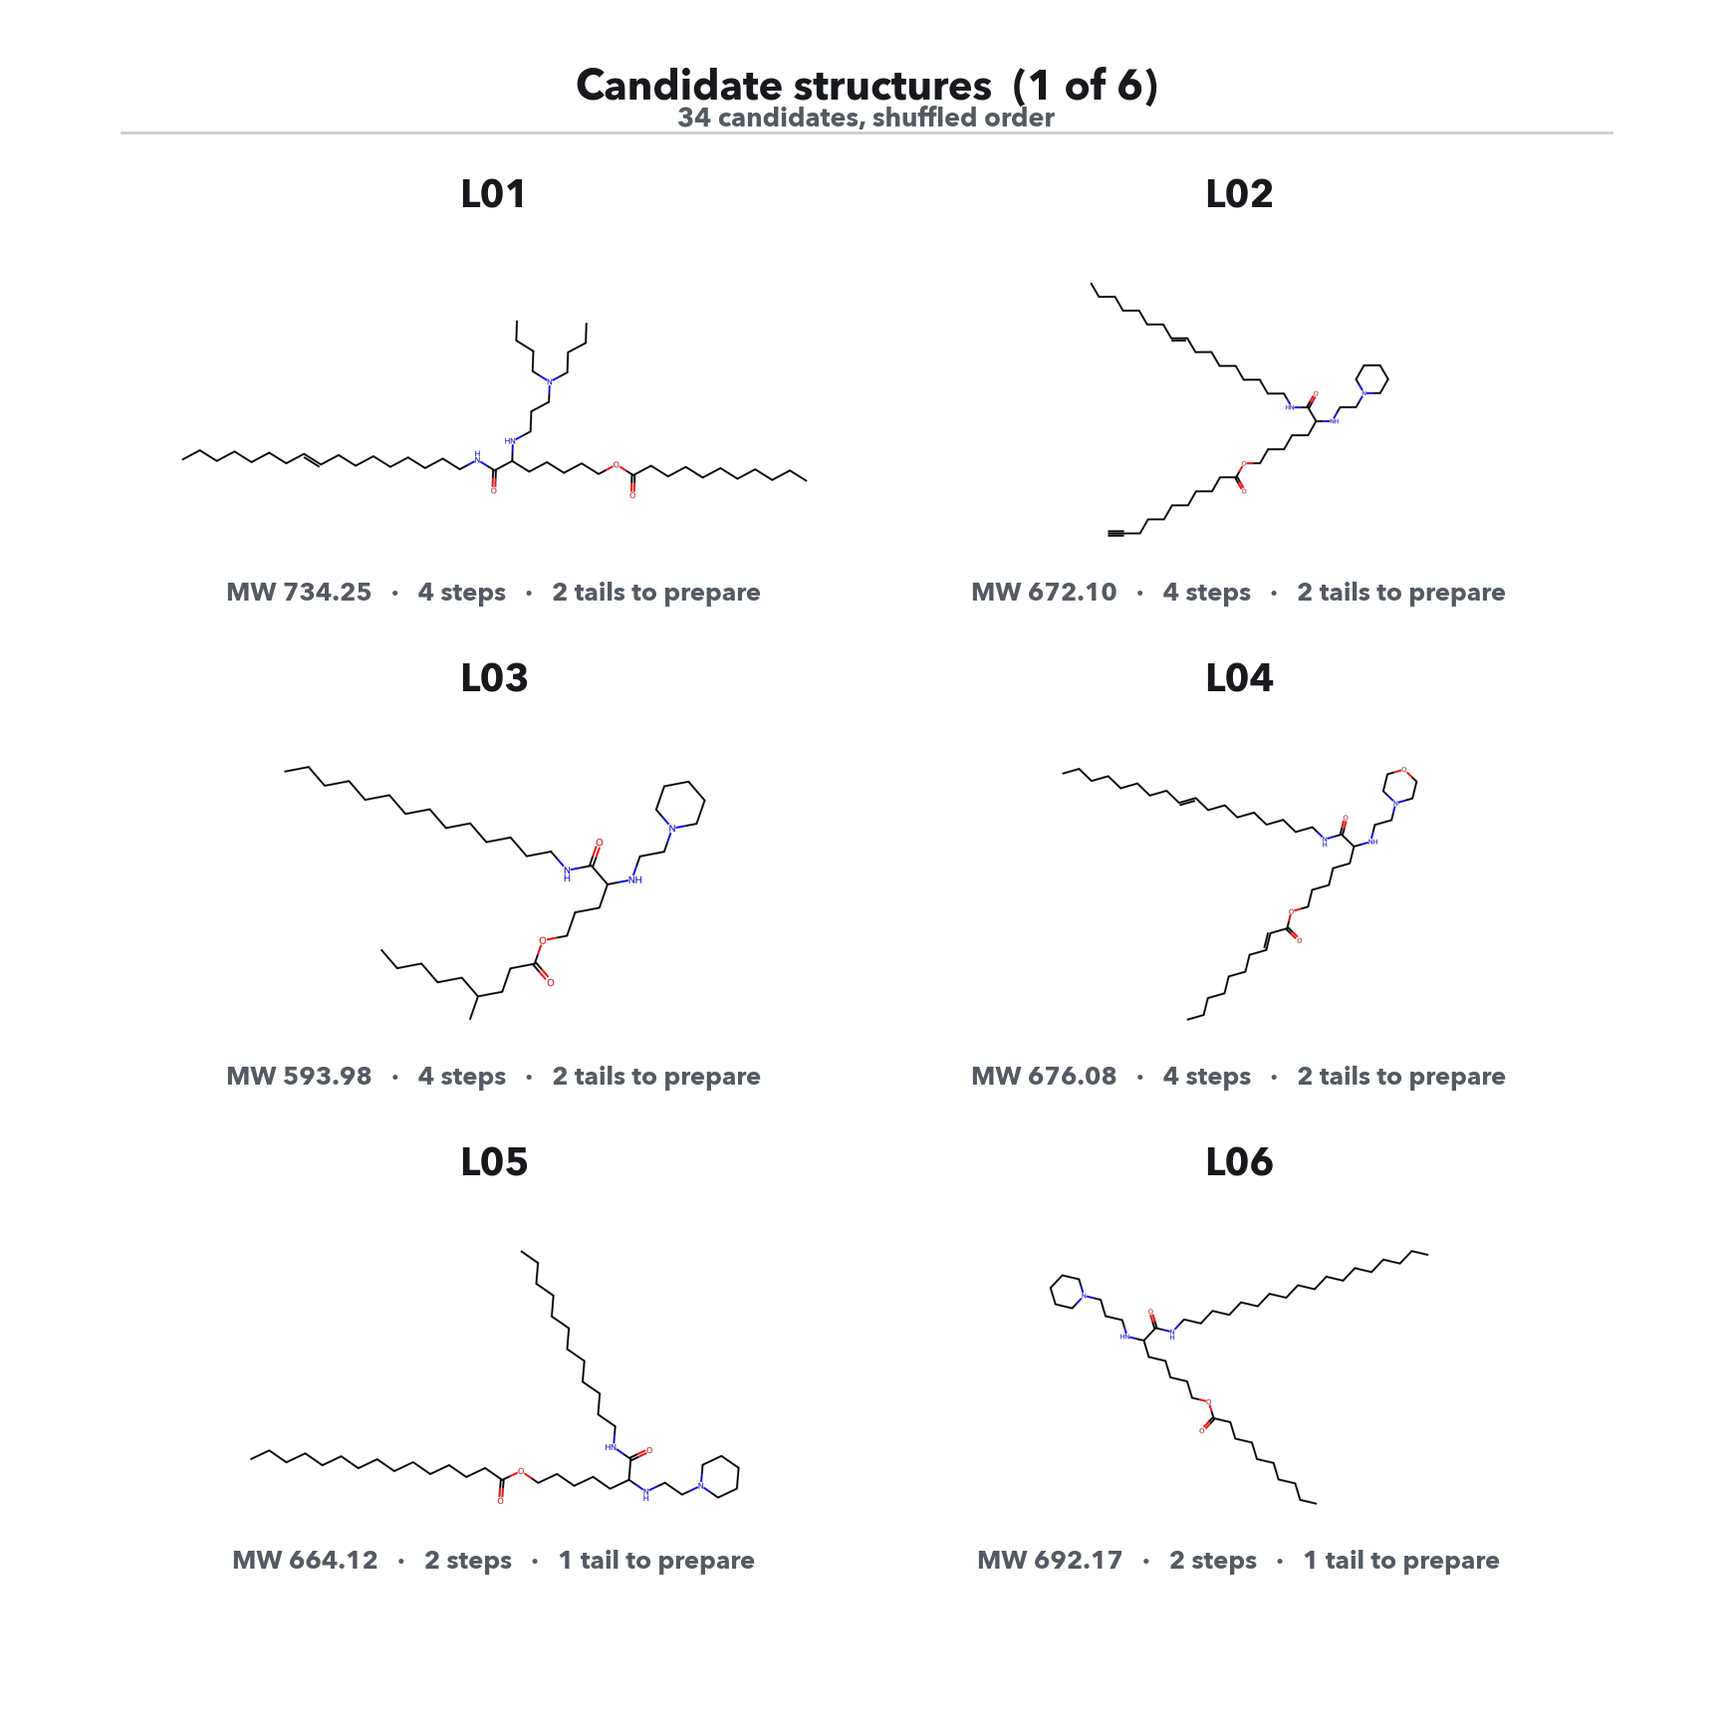
\includegraphics[width=0.72\textwidth]{chemist_packet/dossier_structures.png}
\caption{\textbf{Blinded dossier, candidate structures.} One of six structure pages supplied to the
reviewing chemist. Designs carry shuffled codes rather than the rank-ordered pool identifiers, and
no predicted activity, calibrated bound, evidence stratum or arm appears anywhere in the packet.
Native aspect is square.}
\label{fig:dossier-structures}
\end{figure}

\begin{figure}[h]
\centering
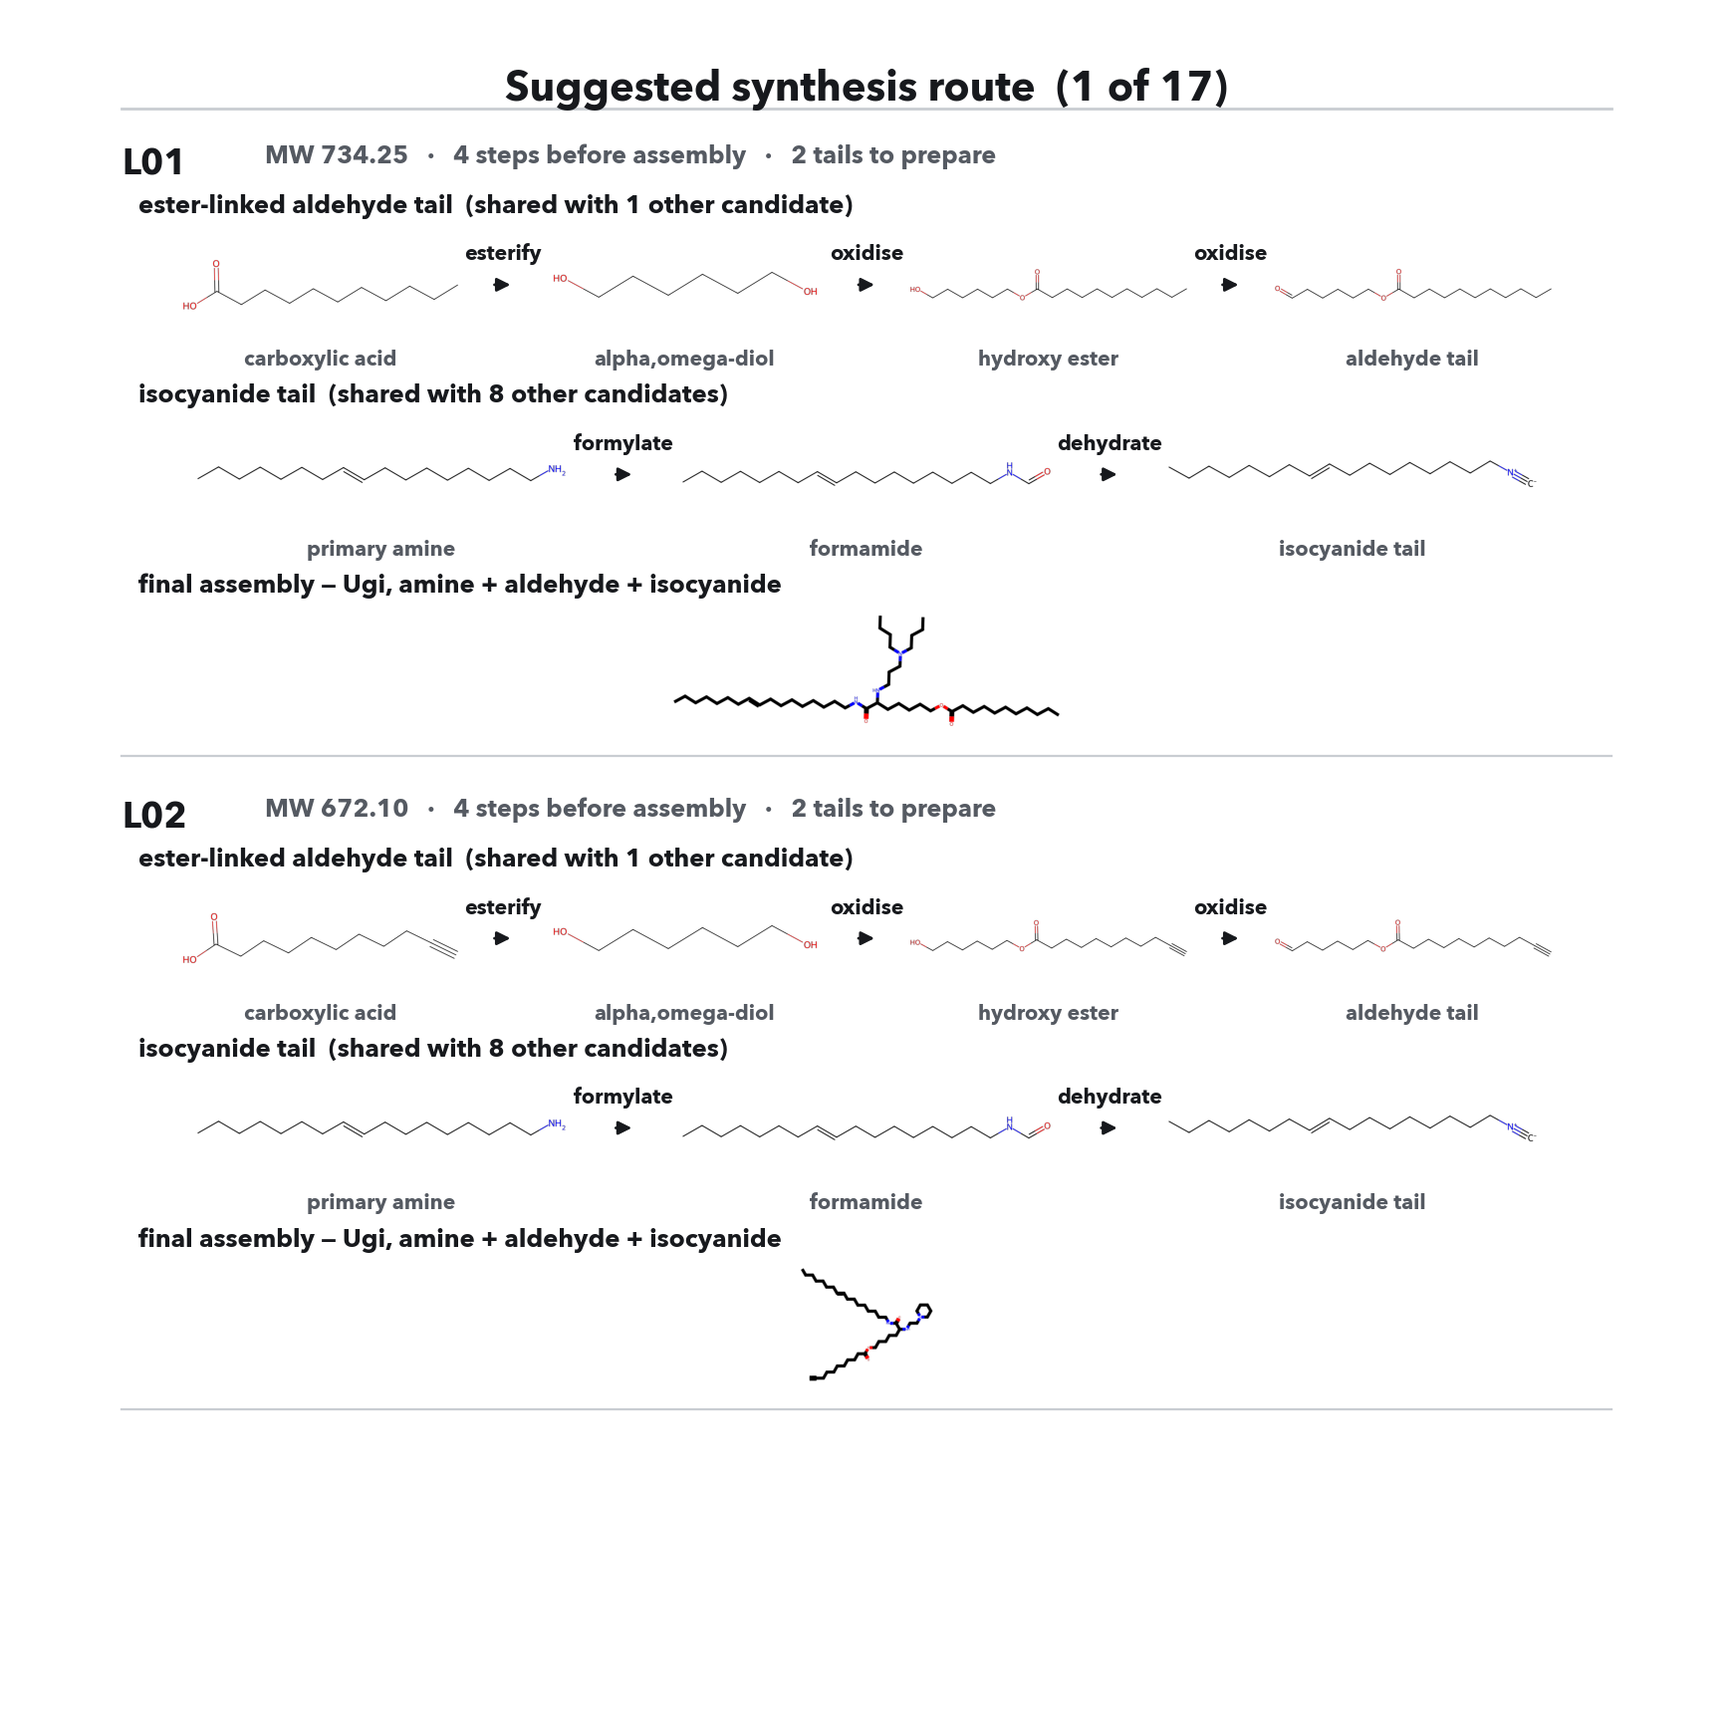
\includegraphics[width=0.72\textwidth]{chemist_packet/dossier_synthesis_route.png}
\caption{\textbf{Blinded dossier, suggested route.} One route page of seventeen. Intermediates are
derived per component and retained only where carrying them forward returns the target structure
exactly. Components shared with other candidates are marked, since one tail preparation can serve
several designs.}
\label{fig:dossier-route}
\end{figure}

\begin{figure}[h]
\centering
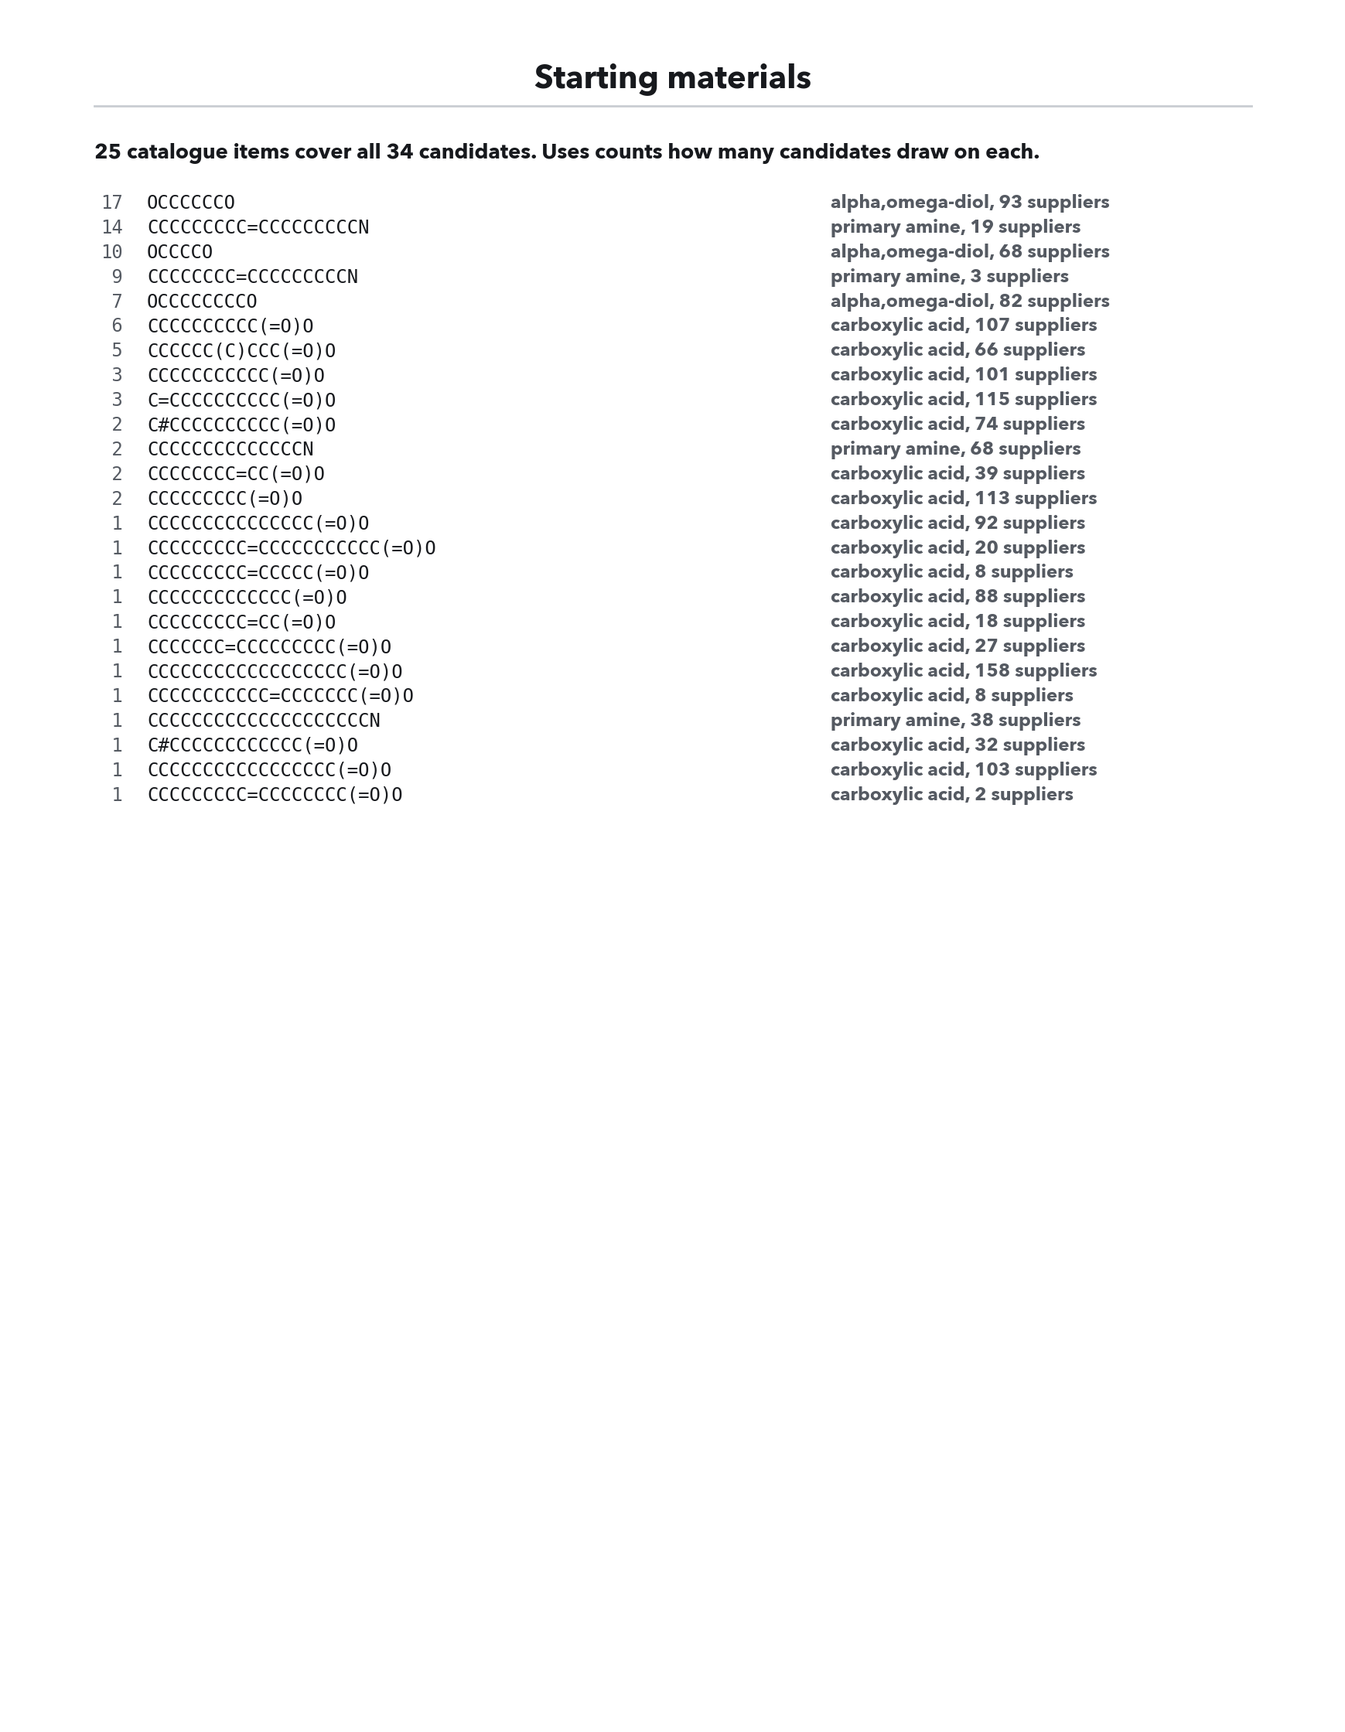
\includegraphics[width=0.62\textwidth]{chemist_packet/dossier_starting_materials.png}
\caption{\textbf{Blinded dossier, consolidated starting materials.} The reviewed designs draw on a
small shared pool of catalogue items, so preparation effort is not proportional to candidate count.
Native aspect is portrait, 1739x2240.}
\label{fig:dossier-materials}
\end{figure}

Synthetic capacity rather than computational throughput limits a prospective campaign, so a subset of
the frozen pool was selected for synthesis by a reviewing chemist. The review took place after the
candidate lock and before any synthesis was attempted, so no experimental outcome informed it.

Table~\ref{tab:blinding} lists what was disclosed and what was withheld, and
Figures~\ref{fig:dossier-structures}--\ref{fig:dossier-materials} reproduce representative pages of
the packet as delivered. The blinding is not a formality. Predicted activity had already determined
which designs entered the pool, so withholding it during the review is what makes the chemistry
selection something other than a second application of the model's own ranking. The pool identifiers
were withheld for the same reason: they are ordered by rank and would have conveyed the ranking on
their own. Codes were assigned in shuffled order under a recorded seed, and the map from code to
identifier was held separately and not supplied with the review materials. The six low-ranked controls
were withheld entirely, because presenting them would have disclosed that a ranking existed.

No structural-diversity target, quota or coverage requirement was imposed. Any such constraint would
be a constraint the model did not choose, and it would have to be described as part of the selection
rule; leaving the selection unconstrained means the structures and their chemistry were the only
inputs to the decision.
\TODO{F.8: the reviewing chemist's identity and affiliation, which candidates were selected, any
adjustment made before the freeze together with its stated reason, and the disposition of the
controls}

\subsection{Historical Library~0 prioritization protocol}
\label{app:library-zero}

\begin{figure}[p]
\centering
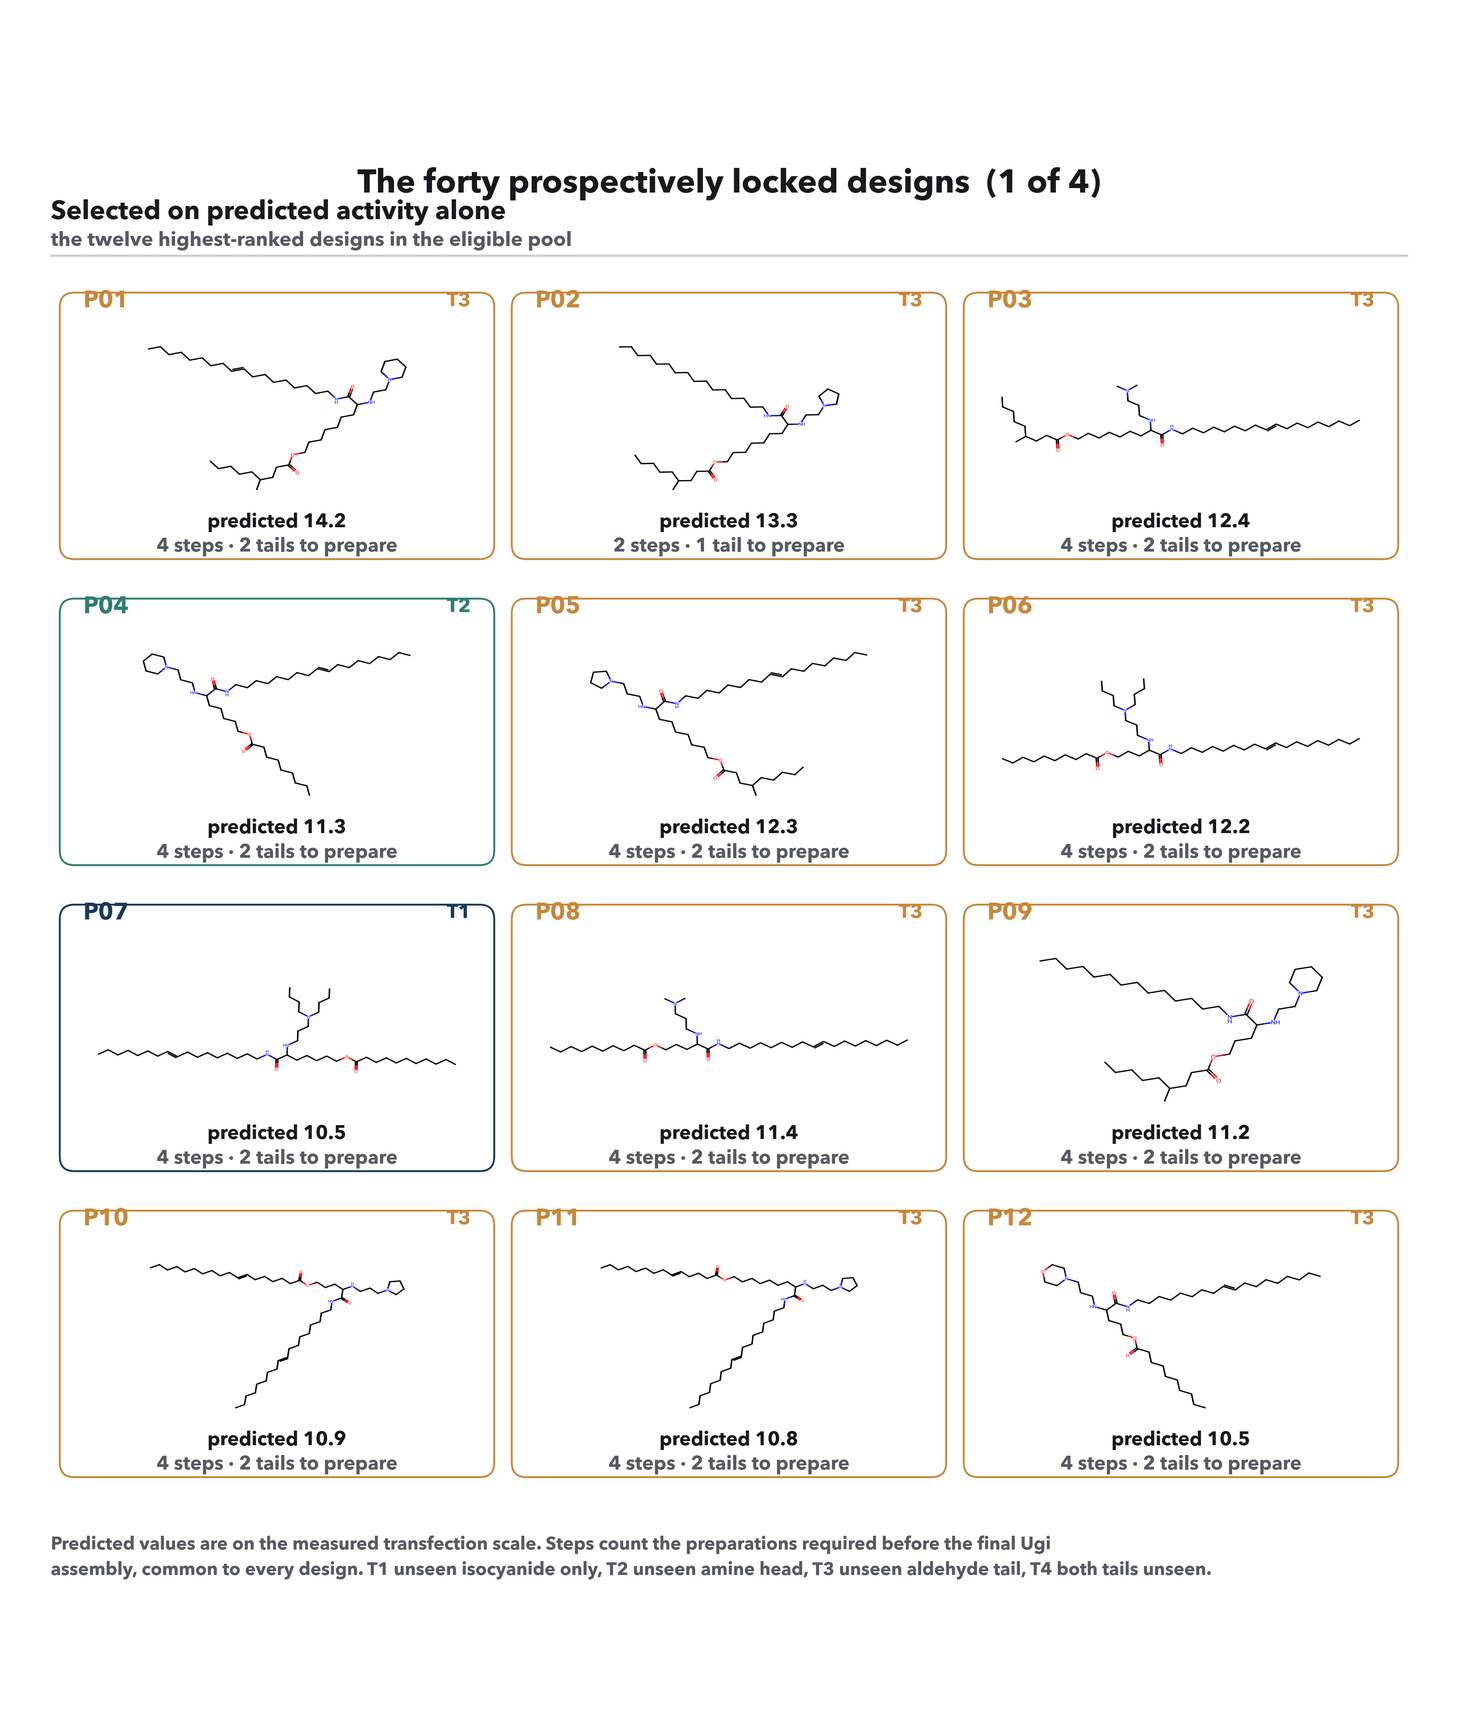
\includegraphics[width=\textwidth]{panel_v6/panel_40_structures_p1.png}
\caption{\textbf{The frozen Library~0 pilot, structures 1 of 4.} Predicted values and the T1--T4
tier badges come from the lower-bound prioritization rule described in this section and are not
current ranking quantities.}
\label{fig:panel-p1}
\end{figure}

\begin{figure}[p]
\centering
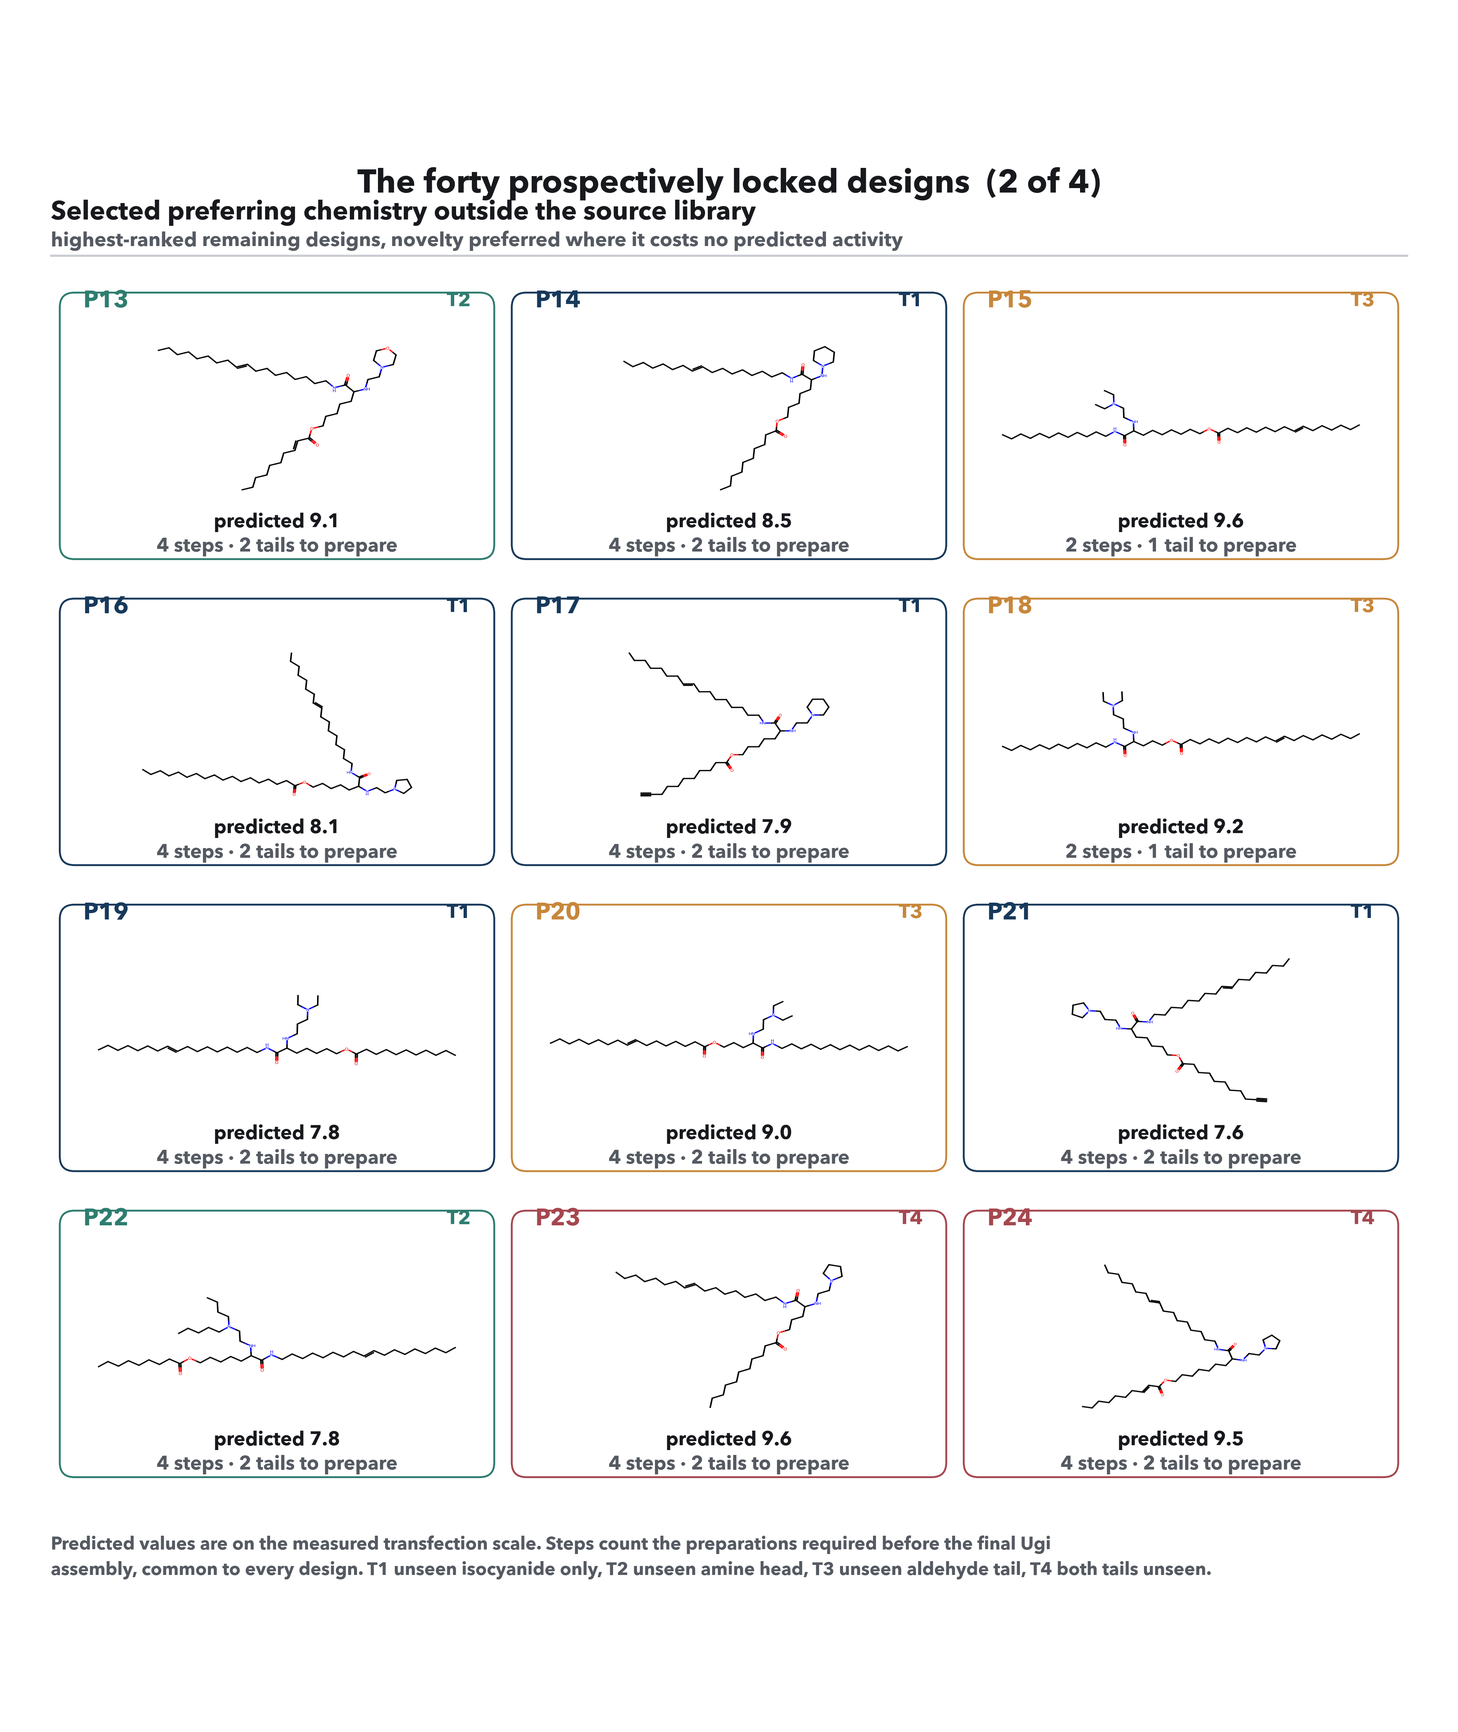
\includegraphics[width=\textwidth]{panel_v6/panel_40_structures_p2.png}
\caption{\textbf{The frozen Library~0 pilot, structures 2 of 4.}}
\label{fig:panel-p2}
\end{figure}

\begin{figure}[p]
\centering
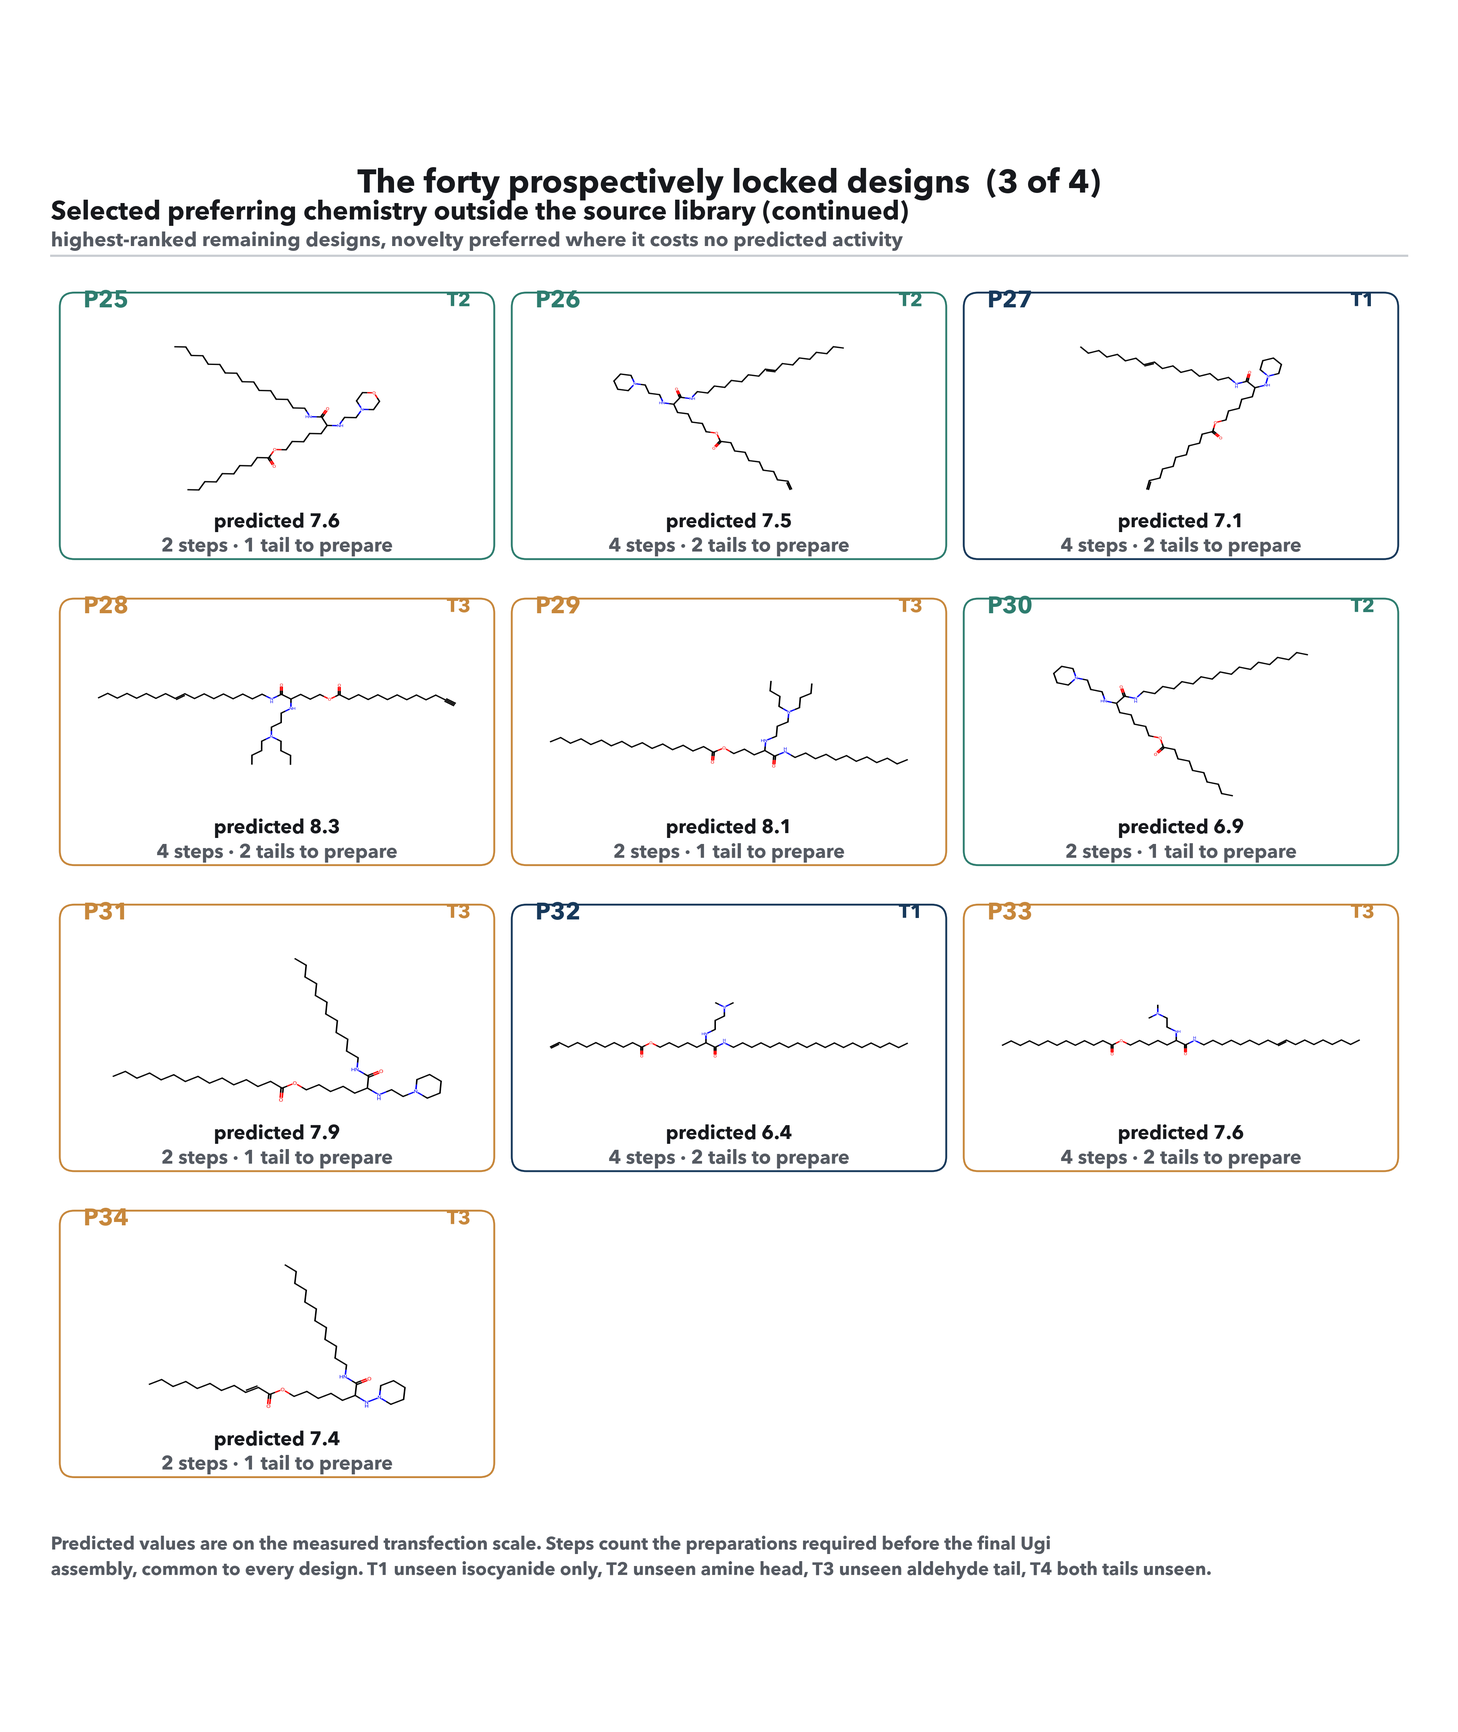
\includegraphics[width=\textwidth]{panel_v6/panel_40_structures_p3.png}
\caption{\textbf{The frozen Library~0 pilot, structures 3 of 4.}}
\label{fig:panel-p3}
\end{figure}

\begin{figure}[p]
\centering
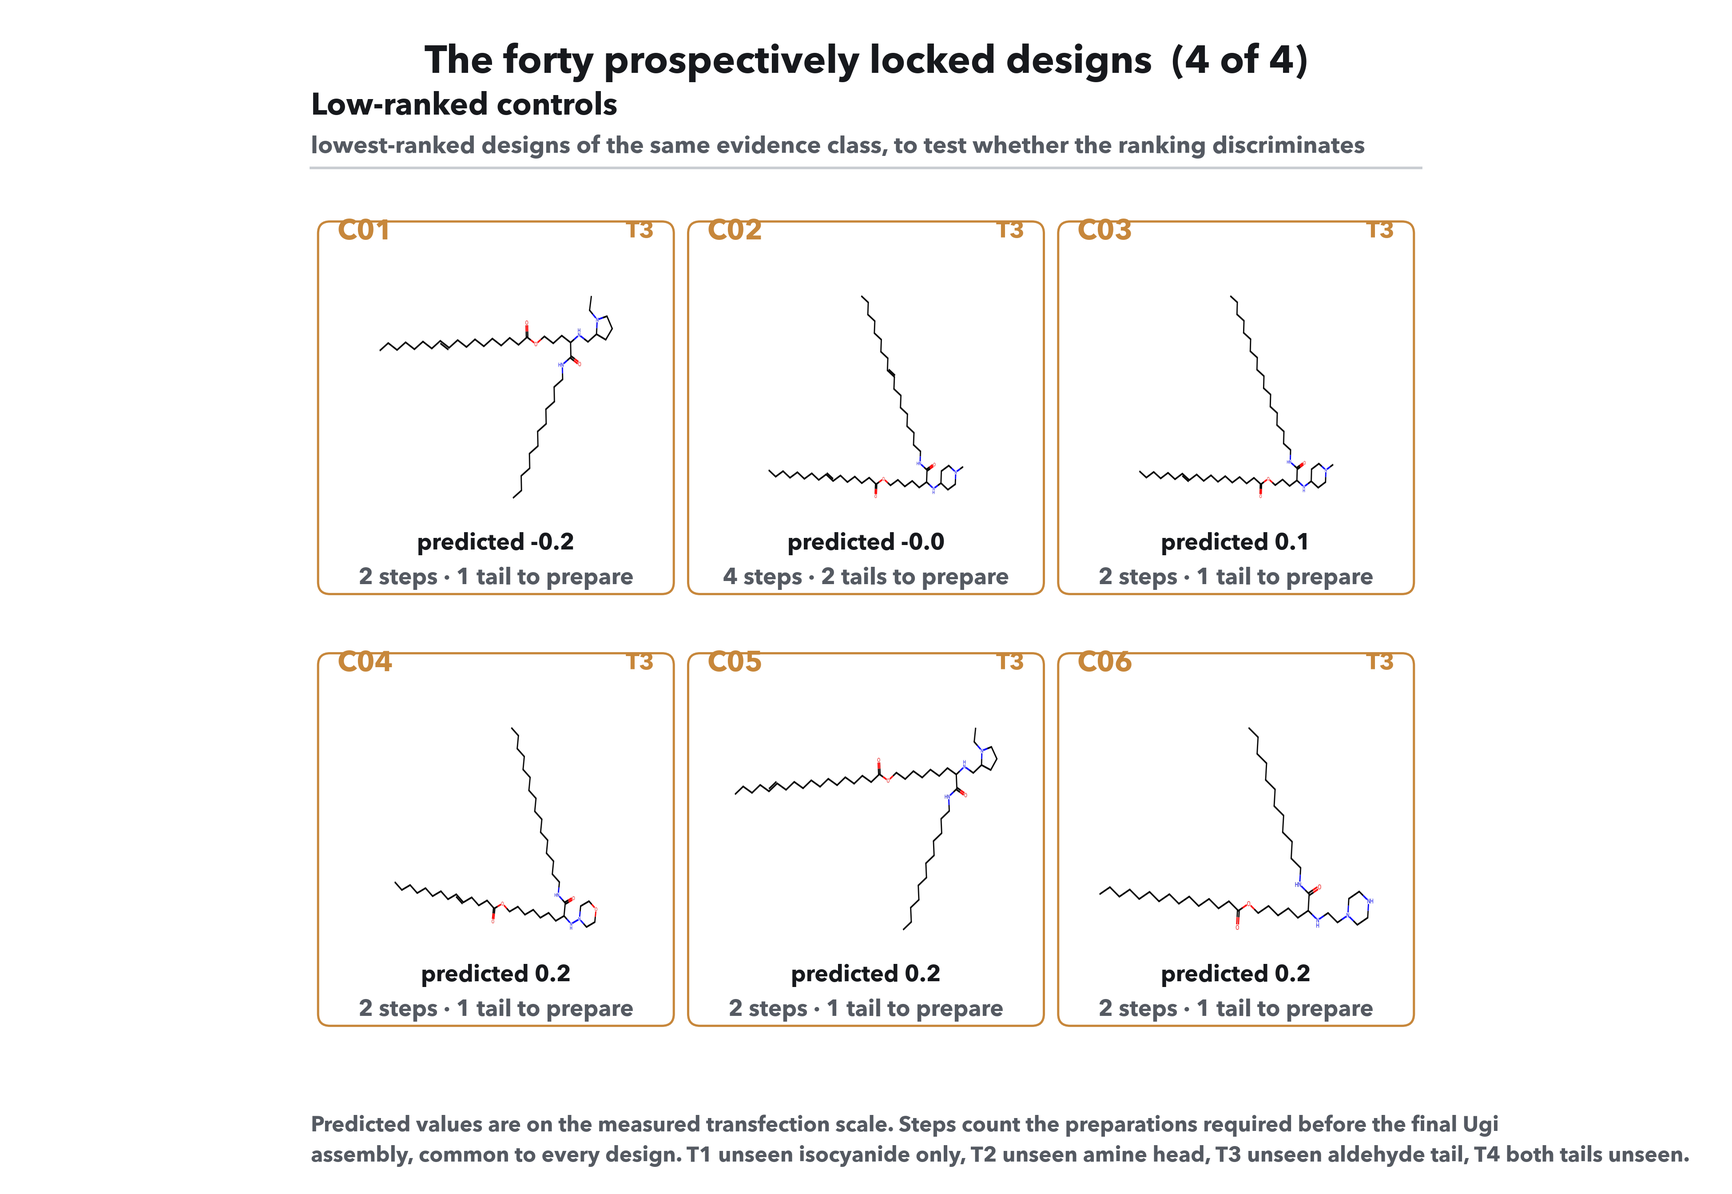
\includegraphics[width=\textwidth]{panel_v6/panel_40_structures_p4.png}
\caption{\textbf{The frozen Library~0 pilot, structures 4 of 4.} This page carries the remaining
high-ranked designs together with the six low-ranked controls, so it is landscape where the first
three pages are portrait.}
\label{fig:panel-p4}
\end{figure}

\emph{This protocol generated the frozen Library~0 computational pilot. It is documented here
because a frozen selection whose rule is unpublished cannot be audited. It is not the ranking used in
the current formulation, and \S\ref{app:lcb-ranking} sets out how the two differ and why neither can be
shown superior without prospective outcomes.}

The rule that produced the pilot is recorded here in full, because a frozen selection whose rule is
not published cannot be audited. Eligibility required valid molecular and Ugi reconstruction, a
calibrated activity estimate, route closure within four upstream steps, membership of the frozen
physicochemical envelope, and absence from the generative training fold. Ranking used the 90\%
conformal lower bound. The twelve highest-ranked eligible designs were taken directly; the remaining
twenty-two of the high arm preferred designs absent from the enumerated library, applied only where
that preference did not lower the ranking; six low-ranked controls were drawn from the lowest-ranked
members of the tail-generalization stratum so that the controls match the bulk of the high arm in
evidence class. Diversity was enforced at a maximum pairwise product Tanimoto of 0.95 and at most four
candidates per amine head, with ties broken deterministically on canonical product SMILES. Tables S2,
S6 and S8 give the resulting panel and rule; Table S17 gives the product structures.

The ranking statistic is where this rule and the current formulation part company, and
\S\ref{app:lcb-ranking} treats that comparison in full: the two rules share \RankShared{} of 34
candidates, and neither can be shown superior without prospective outcomes. Support, ranking and
uncertainty are separate objects in \S\ref{sec:deployment} so that no single statistic has to express
all three at once. The pilot stands as provenance: no member has been synthesized, all forty are
route-complete, and \LibraryZeroUnique{} of \LibraryZeroN{} uniquely assemble.

% =============================================================================
\section{Derivations}
\label{app:derivations}
% =============================================================================


\subsection{Exact component projection}
\label{app:decomp-prop}
Decomposition is not a learned inverse and not a retrosynthetic search. It is a partition of the
terminal state induced by a map the design context already fixes.

\begin{proposition}[Exact component projection]
\label{prop:decomp}
Let $G$ be a terminal state instantiated under design context $c$, with role map
$r_c : V \rightarrow \mathcal{K}_{\mathcal{R}} \cup \{\mathrm{core}\}$. Then $\decomp(G,c)$ is
computable in $O(|V| + |E|)$ time consulting no external resource, and if $A_{\mathcal{R}}(G,c) = 1$
then $\mathcal{R}(\decomp(G,c)) \cong G$.
\end{proposition}

\begin{proof}
The map $r_c$ partitions $V$ into the three role blocks and the shared core. Each edge of $E$ is
classified by the roles of its endpoints in one pass, giving intra-role edges, intra-core edges, and
the cut edges crossing a role boundary at the core. For role $k$, take the subgraph induced on
$r_c^{-1}(k)$ together with its core attachment atoms, and close each cut edge with the valence
$\mathcal{R}$ assigns to that attachment. Both the classification and the closure visit each vertex
and edge once, so the projection is linear and involves no catalogue, no template library and no
search. The second claim is immediate: $A_{\mathcal{R}}(G,c) = 1$ requires by definition that
$\mathcal{R}(\decomp(G,c)) \cong G$, so certification costs one canonicalization and one graph
isomorphism test rather than a route search.
\end{proof}

Two things are worth separating here. The projection is exact by construction, because $r_c$ is
supplied rather than inferred; this is what makes the decomposition available before generation
rather than recovered after it. What the proposition does not give is procurement: it says the three
components are determined and reassemble the product, not that any of them can be obtained. That is
Appendix~\ref{app:synthesis}.

\subsection{The evidence-aware proposal is a KL-regularized tilt}
\label{app:kl-derivation}
Write $f(c) = \log(\rho(c) + \epsilon)$ and consider
%
\[
\mathcal{J}(q) = \mathbb{E}_{c \sim q}\!\left[ f(c) \right]
- \frac{1}{\gamma} D_{\mathrm{KL}}\!\left( q \,\|\, \pi_0 \right),
\qquad \gamma > 0,
\]
%
maximized over distributions $q$ on the countable context set. Introducing a multiplier $\mu$ for
$\sum_c q(c) = 1$ and differentiating the Lagrangian with respect to $q(c)$ gives
%
\[
f(c) - \frac{1}{\gamma}\left( \log \frac{q(c)}{\pi_0(c)} + 1 \right) - \mu = 0,
\]
%
so $\log q(c) = \log \pi_0(c) + \gamma f(c) + \text{const}$, and therefore
%
\[
q^{*}(c) \;\propto\; \pi_0(c)\, e^{\gamma f(c)} \;=\; \pi_0(c)\, \bigl(\rho(c) + \epsilon\bigr)^{\gamma}.
\]
%
Normalizing recovers $\pi_\gamma$ exactly as defined in Eq.~\eqref{eq:tilt}. Since $\mathcal{J}$ is
strictly concave in $q$ and the constraint set is convex, this stationary point is the unique
maximizer. The exponent $\gamma$ is therefore not a free tuning knob layered on top of the
proposal: it is the inverse temperature of an explicit trade-off between supported yield and
divergence from the broad exploratory proposal.

\subsection{Support preservation, and why it is not diversity preservation}
\label{app:support-preservation}
\begin{proposition}
\label{prop:support}
For any $\epsilon > 0$ and finite $\gamma \geq 0$,
$\operatorname{supp}(\pi_\gamma) = \operatorname{supp}(\pi_0)$.
\end{proposition}

\begin{proof}
For every context $c$ we have $\rho(c) + \epsilon \geq \epsilon > 0$, so
$(\rho(c) + \epsilon)^{\gamma} > 0$ for finite $\gamma$. The normalizing sum in Eq.~\eqref{eq:tilt}
is finite and strictly positive, hence $\pi_\gamma(c) > 0$ if and only if $\pi_0(c) > 0$.
\end{proof}

The proposition is what prevents evidence-aware deployment from silently becoming a support
restriction: no architecture is made impossible. It says nothing at all about how probability mass
is distributed within that support, and the empirical concentration is substantial. Effective
amine-head diversity falls by \AmineDiversityDrop{} under the enriched proposal, while effective
aldehyde-tail diversity is essentially unchanged at \AldehydeDiversityRatio{} times its unenriched
value.

The mechanism behind that asymmetry is worth naming, because it is a property of the evidence
rather than of the tilt. Membership of \Spred{} requires \emph{all four} views to pass, and the
measured library is far denser at the amine head than at either tail: 20 measured heads against
\AmineReg{} in the corpus registry, compared with 11 measured aldehydes against \AldehydeReg{}.
Tilting toward support therefore pulls hardest on the role where the reference chemistry is most
concentrated, which is why head diversity absorbs almost all of the loss while the aldehyde tail is
left essentially untouched. A tilt that concentrated on the tails instead would require a measured
library with the opposite shape.

\subsection{Sampler support invariant}
\label{app:sampler-invariant}

\begin{proposition}[Sampler support invariant]
\label{prop:sampler}
If the initial partial state is admissible and every mask assigns zero probability to any successor
violating a declared bound, then every state reached during sampling, including the terminal state,
lies in $\Sgen(c)$.
\end{proposition}

\begin{proof}
By induction on the transition index $n$. At $n = 0$ the initial partial state is admissible by
assumption. Suppose the state after $n$ transitions is admissible. Each mask is a predicate on
candidate successors evaluated against the declared bounds: valence masks forbid an atom exceeding
its allowed degree, duplicate-edge and self-edge masks forbid a multigraph or a loop, the
adapter-boundary mask forbids an edge crossing a role boundary anywhere but the core, and the
counting masks forbid exceeding the per-component atom, child, junction, cycle and core-attachment
budgets. Every successor assigned nonzero probability therefore satisfies the bounds and retains a
completion within them, so the state after $n+1$ transitions is admissible. Sampling terminates
after finitely many transitions at a state with no pending frontier, and that state is admissible,
hence in $\Sgen(c)$.
\end{proof}

This is a property of the sampler, not a learned capability of the model. A nonlearned role-marginal
sampler operating under the same masks satisfies it identically, which is exactly why declared
support cannot be offered as evidence that the model has learned lipid chemistry, and why the
marginal-null contrast of \S\ref{sec:res-fidelity} is needed.

% =============================================================================
\section{Prospective Experimental Protocol}
\label{app:prospective}
% =============================================================================
% scaffold - fill in after the campaign actually runs, no generic boilerplate
\PENDING{PROSPECTIVE PROTOCOL PENDING EXECUTION}

\subsection{Prespecified reporting table}
\label{app:reporting-skeleton}
Rows are the designs selected by the chemistry review, in the order fixed before any experiment.
No row is added, removed or reordered once synthesis begins, and a design that fails at any stage
keeps its row with the failure recorded against it. The table ships blank: a prespecified reporting
frame is what makes the campaign legible as prospective rather than narrated after the fact.

\begin{table}[h]
\centering
\caption{Prespecified reporting frame. Row order is fixed before synthesis begins.}
\label{tab:reporting-frame}
\scriptsize
\begin{tabular}{@{}lccccccc@{}}
\toprule
Design & Precursors & Final & Identity & LNP & Size, & Encapsu- & HeLa / \\
       & prepared   & assembly & and purity & formed & PDI & lation & viability \\
\midrule
1 & & & & & & & \\
2 & & & & & & & \\
3 & & & & & & & \\
4 & & & & & & & \\
5 & & & & & & & \\
6 & & & & & & & \\
7 & & & & & & & \\
8 & & & & & & & \\
9 & & & & & & & \\
10 & & & & & & & \\
11 & & & & & & & \\
12 & & & & & & & \\
\bottomrule
\end{tabular}
\end{table}

Matched-reference comparisons are recorded alongside each row where a matched reference exists.

\subsection{Protocol}
\label{app:protocol}

\TODO{H.3: candidate-freeze date and hash; selection protocol; matched-reference construction;
synthesis and purification; structural characterization; LNP formulation composition and
procedure; encapsulation measurement; particle size and PDI; cell line and culture conditions;
mRNA dose; treatment duration; reporter assay; viability assay; the definition of technical
versus biological replicate; positive and negative controls; randomization and blinding if used;
the primary endpoint; the prespecified statistical test; the handling of failed synthesis or
formulation; \emph{in vivo} methods and ethics or animal approvals if applicable.}

% =============================================================================
\section{Generated Data Tables}
\label{app:datatables}
% =============================================================================

% autogenerated - regenerate, dont edit directly

\subsection{Per-head and per-seed semantic results}
\label{app:sem-tables}
\begin{table}[h]
\centering
\small
\caption{\textbf{Semantic-utility gap per head and per paired seed.} Each entry is $L_{\text{no-role}} - L_{\text{true-role}}$ for that head, within the seed's paired run, so positive means the aligned map reconstructs better. The six rows above the rule are the semantic pilot's reported set, matching PRIMARY\_HEADS in the closure script. Below it are the two heads belonging only to the role-divergence analysis, a different six; those two are not uniformly positive and no claim is made over them.}
\label{tab:sem-per-head}
\begin{tabular}{@{}lrrrrrc@{}}
\toprule
head & s1 & s2 & s3 & mean & s.d. & all positive \\
\midrule
atom state & +0.0282 & +0.0261 & +0.0254 & +0.0266 & 0.0015 & yes \\
parent bond & +0.0189 & +0.0148 & +0.0175 & +0.0170 & 0.0021 & yes \\
offspring topology & +0.1402 & +0.1439 & +0.1386 & +0.1409 & 0.0027 & yes \\
closure bond & +0.0172 & +0.0146 & +0.0195 & +0.0171 & 0.0025 & yes \\
decoration anchor & +0.0501 & +0.0417 & +0.0400 & +0.0439 & 0.0054 & yes \\
\midrule
\textbf{total} & +0.2956 & +0.1835 & +0.2646 & +0.2479 & 0.0579 & yes \\
\midrule
\multicolumn{6}{@{}l}{\emph{Heads used only by the role-divergence analysis of Amendment 14, not part of the six above:}} \\
decoration atom & +0.0054 & -0.0022 & +0.0052 & +0.0028 & 0.0043 & \textbf{2/3} \\
decoration bond & +0.0355 & -0.0554 & +0.0185 & -0.0005 & 0.0483 & \textbf{2/3} \\
\bottomrule
\end{tabular}
\end{table}

\begin{table}[h]
\centering
\small
\caption{\textbf{Corruption dependence of the semantic-utility gap.} The gap near the corrupted end of the probability path, against the gap near the clean endpoint, per seed. The direction replicates in every seed; the magnitude does not, which is why the three values are reported rather than a range.}
\label{tab:sem-corruption}
\begin{tabular}{@{}lrrr@{}}
\toprule
seed & gap, corrupted end & gap, clean end & ratio \\
\midrule
s1 & +0.5126 & +0.0666 & 7.70$\times$ \\
s2 & +0.3206 & +0.0324 & 9.89$\times$ \\
s3 & +0.4617 & +0.0410 & 11.25$\times$ \\
\bottomrule
\end{tabular}
\end{table}

\begin{table}[h]
\centering
\small
\caption{\textbf{The misalignment control.} Denoising loss under the three arms; lower is better. A negative \emph{none $-$ misaligned} means the misaligned arm is \emph{worse} than receiving no role at all, which is what rules out attributing the benefit to the presence of an extra categorical channel.}
\label{tab:sem-misaligned}
\begin{tabular}{@{}lrrrrr@{}}
\toprule
head & true & none & misaligned & none $-$ mis. & true $-$ mis. \\
\midrule
atom state & 0.1180 & 0.1463 & 0.1459 & +0.0003 & -0.0279 \\
parent bond & 0.0747 & 0.0935 & 0.0945 & -0.0010 & -0.0198 \\
offspring topology & 0.1648 & 0.3050 & 0.3108 & -0.0057 & -0.1460 \\
closure bond & 0.1235 & 0.1407 & 0.1463 & -0.0056 & -0.0228 \\
decoration anchor & 0.1273 & 0.1775 & 0.1727 & +0.0047 & -0.0454 \\
\midrule
\textbf{total} & 0.8138 & 1.1094 & 1.1149 & -0.0056 & -0.3012 \\
\bottomrule
\end{tabular}
\end{table}

\subsection{The complete descriptor panel}
\label{app:panel-tables}
\begingroup\small
\begin{longtable}{@{}llrrr@{}}
\caption{\textbf{The complete lipid-native descriptor panel.} Median value per descriptor for held-out real lipids, FORGE samples, and the role-marginal null. Every descriptor is reported, not only those on which FORGE compares well: the panel is a guard against post-hoc metric selection only if its unselected members are published. Populations: real $n=3,072$, FORGE $n=2,985$, null $n=3,072$.}\label{tab:panel-full}\\
\toprule
descriptor & region & real & FORGE & null \\
\midrule
\endfirsthead
\toprule descriptor & region & real & FORGE & null \\ \midrule \endhead
\bottomrule
\endfoot
\texttt{ald\_alkenes} & aldehyde tail & 1.000 & 0.000 & 0.000 \\
\texttt{ald\_branches} & aldehyde tail & 0.000 & 0.000 & 0.000 \\
\texttt{ald\_carbons} & aldehyde tail & 15.000 & 15.000 & 16.000 \\
\texttt{ald\_esters} & aldehyde tail & 1.000 & 1.000 & 0.000 \\
\texttt{ald\_ethers} & aldehyde tail & 0.000 & 0.000 & 0.000 \\
\texttt{ald\_heavy\_atoms} & aldehyde tail & 18.000 & 18.000 & 18.000 \\
\texttt{ald\_ketones} & aldehyde tail & 0.000 & 0.000 & 1.000 \\
\texttt{ald\_longest\_chain} & aldehyde tail & 11.000 & 11.000 & 16.000 \\
\texttt{clogp} & whole lipid & 7.694 & 8.175 & 6.762 \\
\texttt{degradable\_linkages} & whole lipid & 1.000 & 1.000 & 0.000 \\
\texttt{hba} & whole lipid & 5.000 & 5.000 & 6.000 \\
\texttt{hbd} & whole lipid & 2.000 & 2.000 & 3.000 \\
\texttt{head\_hba} & ionizable head & 2.000 & 2.000 & 2.000 \\
\texttt{head\_hbd} & ionizable head & 1.000 & 1.000 & 2.000 \\
\texttt{head\_heavy\_atoms} & ionizable head & 9.000 & 9.000 & 10.000 \\
\texttt{head\_max\_n\_spacing} & ionizable head & 3.000 & 3.000 & 0.000 \\
\texttt{head\_min\_n\_spacing} & ionizable head & 3.000 & 2.000 & 0.000 \\
\texttt{head\_nitrogens} & ionizable head & 2.000 & 2.000 & 1.000 \\
\texttt{head\_primary\_amine} & ionizable head & 1.000 & 1.000 & 0.000 \\
\texttt{head\_ring\_nitrogen} & ionizable head & 0.000 & 0.000 & 0.000 \\
\texttt{head\_rings} & ionizable head & 1.000 & 1.000 & 1.000 \\
\texttt{head\_secondary\_amine} & ionizable head & 0.000 & 0.000 & 0.000 \\
\texttt{head\_tertiary\_amine} & ionizable head & 0.000 & 1.000 & 0.000 \\
\texttt{head\_to\_tail\_ratio} & ionizable head & 0.312 & 0.310 & 0.364 \\
\texttt{iso\_alkenes} & isocyanide tail & 0.000 & 0.000 & 0.000 \\
\texttt{iso\_branches} & isocyanide tail & 0.000 & 0.000 & 0.000 \\
\texttt{iso\_carbons} & isocyanide tail & 11.000 & 11.000 & 11.000 \\
\texttt{iso\_esters} & isocyanide tail & 0.000 & 0.000 & 0.000 \\
\texttt{iso\_ethers} & isocyanide tail & 0.000 & 0.000 & 0.000 \\
\texttt{iso\_heavy\_atoms} & isocyanide tail & 13.000 & 12.000 & 14.000 \\
\texttt{iso\_ketones} & isocyanide tail & 0.000 & 0.000 & 1.000 \\
\texttt{iso\_longest\_chain} & isocyanide tail & 8.000 & 8.000 & 8.000 \\
\texttt{molecular\_weight} & whole lipid & 565.821 & 563.956 & 616.840 \\
\texttt{rotatable\_bonds} & whole lipid & 26.000 & 27.000 & 28.000 \\
\texttt{tail\_asymmetry} & whole lipid & 6.000 & 6.000 & 6.000 \\
\texttt{tail\_balance} & whole lipid & 0.578 & 0.571 & 0.579 \\
\texttt{total\_tail\_carbons} & whole lipid & 27.000 & 27.000 & 28.000 \\
\texttt{tpsa} & whole lipid & 70.670 & 70.670 & 129.640 \\
\end{longtable}
\endgroup

\begin{table}[h]
\centering
\small
\caption{\textbf{Grouped real-versus-generated separability.} Grouping is by aldehyde component family, so repeated component combinations cannot leak across folds. Per-fold values are given because the mean alone hides the spread.}
\label{tab:grouped-auc}
\begin{tabular}{@{}lrrl@{}}
\toprule
arm & groups & mean AUC & per-fold AUC \\
\midrule
FORGE & 11 & 0.8820 & 0.852, 0.969, 0.869, 0.883, 0.838 \\
role-marginal null & 11 & 1.0000 & 1.000, 1.000, 1.000, 1.000, 1.000 \\
earlier checkpoint & 11 & 0.9581 & 0.982, 0.992, 0.939, 0.949, 0.928 \\
\bottomrule
\end{tabular}
\end{table}



% =============================================================================
\section{Supplementary Tables}
\label{app:stables}
% =============================================================================

% S1--S16 are GENERATED. Regenerate with
%   scripts/phase1\_build\_manuscript\_supplement\_v1.py

\begingroup\footnotesize
% autogenerated supplement tables - regenerate these, dont edit by hand
All tables are generated from the frozen selection artifact and its pinned inputs. Regenerating this file after any change to the selection is required; the numbers here are not transcribed.

\begin{itemize}
\tightlist
\item
  Selection configuration: \texttt{c\allowbreak{}o\allowbreak{}n\allowbreak{}f\allowbreak{}i\allowbreak{}g\allowbreak{}s\allowbreak{}/\allowbreak{}b\allowbreak{}i\allowbreak{}o\allowbreak{}/\allowbreak{}p\allowbreak{}h\allowbreak{}a\allowbreak{}s\allowbreak{}e\allowbreak{}1\allowbreak{}\_\allowbreak{}u\allowbreak{}g\allowbreak{}i\allowbreak{}\_\allowbreak{}p\allowbreak{}r\allowbreak{}o\allowbreak{}s\allowbreak{}p\allowbreak{}e\allowbreak{}c\allowbreak{}t\allowbreak{}i\allowbreak{}v\allowbreak{}e\allowbreak{}\_\allowbreak{}p\allowbreak{}a\allowbreak{}n\allowbreak{}e\allowbreak{}l\allowbreak{}\_\allowbreak{}v\allowbreak{}6\allowbreak{}.\allowbreak{}j\allowbreak{}s\allowbreak{}o\allowbreak{}n}, sha256 \texttt{0\allowbreak{}e\allowbreak{}0\allowbreak{}4\allowbreak{}c\allowbreak{}1\allowbreak{}7\allowbreak{}d\allowbreak{}a\allowbreak{}a\allowbreak{}7\allowbreak{}e\allowbreak{}6\allowbreak{}8\allowbreak{}a\allowbreak{}7}
\item
  Panel artifact: \texttt{r\allowbreak{}e\allowbreak{}s\allowbreak{}u\allowbreak{}l\allowbreak{}t\allowbreak{}s\allowbreak{}/\allowbreak{}p\allowbreak{}h\allowbreak{}a\allowbreak{}s\allowbreak{}e\allowbreak{}1\allowbreak{}/\allowbreak{}u\allowbreak{}g\allowbreak{}i\allowbreak{}\_\allowbreak{}p\allowbreak{}r\allowbreak{}o\allowbreak{}s\allowbreak{}p\allowbreak{}e\allowbreak{}c\allowbreak{}t\allowbreak{}i\allowbreak{}v\allowbreak{}e\allowbreak{}\_\allowbreak{}p\allowbreak{}a\allowbreak{}n\allowbreak{}e\allowbreak{}l\allowbreak{}\_\allowbreak{}v\allowbreak{}6\allowbreak{}/\allowbreak{}p\allowbreak{}r\allowbreak{}o\allowbreak{}s\allowbreak{}p\allowbreak{}e\allowbreak{}c\allowbreak{}t\allowbreak{}i\allowbreak{}v\allowbreak{}e\allowbreak{}\_\allowbreak{}p\allowbreak{}a\allowbreak{}n\allowbreak{}e\allowbreak{}l\allowbreak{}.\allowbreak{}j\allowbreak{}s\allowbreak{}o\allowbreak{}n\allowbreak{}l\allowbreak{}.\allowbreak{}g\allowbreak{}z}, sha256 \texttt{d\allowbreak{}9\allowbreak{}b\allowbreak{}7\allowbreak{}c\allowbreak{}0\allowbreak{}a\allowbreak{}7\allowbreak{}0\allowbreak{}c\allowbreak{}8\allowbreak{}d\allowbreak{}8\allowbreak{}5\allowbreak{}2\allowbreak{}8}
\item
  Derived numbers: \texttt{r\allowbreak{}e\allowbreak{}s\allowbreak{}u\allowbreak{}l\allowbreak{}t\allowbreak{}s\allowbreak{}/\allowbreak{}p\allowbreak{}h\allowbreak{}a\allowbreak{}s\allowbreak{}e\allowbreak{}1\allowbreak{}/\allowbreak{}u\allowbreak{}g\allowbreak{}i\allowbreak{}\_\allowbreak{}m\allowbreak{}a\allowbreak{}n\allowbreak{}u\allowbreak{}s\allowbreak{}c\allowbreak{}r\allowbreak{}i\allowbreak{}p\allowbreak{}t\allowbreak{}\_\allowbreak{}n\allowbreak{}u\allowbreak{}m\allowbreak{}b\allowbreak{}e\allowbreak{}r\allowbreak{}s\allowbreak{}\_\allowbreak{}v\allowbreak{}1\allowbreak{}/\allowbreak{}r\allowbreak{}e\allowbreak{}s\allowbreak{}u\allowbreak{}l\allowbreak{}t\allowbreak{}.\allowbreak{}j\allowbreak{}s\allowbreak{}o\allowbreak{}n}, sha256 \texttt{3\allowbreak{}2\allowbreak{}e\allowbreak{}1\allowbreak{}e\allowbreak{}0\allowbreak{}0\allowbreak{}e\allowbreak{}b\allowbreak{}3\allowbreak{}e\allowbreak{}7\allowbreak{}9\allowbreak{}2\allowbreak{}5\allowbreak{}6}
\end{itemize}

\subsection{Table S1 \textbar{} Evidence tiers and what each one assumes}\label{table-s1-evidence-tiers-and-what-each-one-assumes}

The activity model issues a calibrated interval for every candidate in the panel, but the evidence behind those intervals is not uniform. Tiers are assigned by which component identities were absent from the measured training set, and are recorded per candidate. The panel is not powered for per-tier claims; the tier is reported so that an outcome can be read against the evidence supporting it.

{\def\LTcaptype{none} % do not increment counter
\begin{longtable}[]{@{}
  >{\raggedright\arraybackslash}p{(\linewidth - 10\tabcolsep) * \real{0.1667}}
  >{\raggedright\arraybackslash}p{(\linewidth - 10\tabcolsep) * \real{0.1667}}
  >{\raggedright\arraybackslash}p{(\linewidth - 10\tabcolsep) * \real{0.1667}}
  >{\raggedright\arraybackslash}p{(\linewidth - 10\tabcolsep) * \real{0.1667}}
  >{\raggedright\arraybackslash}p{(\linewidth - 10\tabcolsep) * \real{0.1667}}
  >{\raggedright\arraybackslash}p{(\linewidth - 10\tabcolsep) * \real{0.1667}}@{}}
\toprule\noalign{}
\begin{minipage}[b]{\linewidth}\raggedright
Tier
\end{minipage} & \begin{minipage}[b]{\linewidth}\raggedright
Component absent from the measured set
\end{minipage} & \begin{minipage}[b]{\linewidth}\raggedright
Panel
\end{minipage} & \begin{minipage}[b]{\linewidth}\raggedright
High arm
\end{minipage} & \begin{minipage}[b]{\linewidth}\raggedright
Low arm
\end{minipage} & \begin{minipage}[b]{\linewidth}\raggedright
Eligible pool
\end{minipage} \\
\midrule\noalign{}
\endhead
\bottomrule\noalign{}
\endlastfoot
T1 qualified role holdout & isocyanide only & 8 & 8 & 0 & 119 \\
T2 head generalization & amine head & 6 & 6 & 0 & 24 \\
T3 tail generalization & aldehyde tail & 24 & 18 & 6 & 671 \\
T4 dual tail generalization & aldehyde and isocyanide & 2 & 2 & 0 & 553 \\
\textbf{Total} & & \textbf{40} & \textbf{34} & \textbf{6} & \textbf{1367} \\
\end{longtable}
}

\textbf{T1 qualified role holdout.} Every component except the isocyanide appears in the measured training set, and the isocyanide identity was held out during model fitting. The activity model was validated on exactly this kind of substitution, so its calibrated interval carries the most direct evidence available in the panel.

\textbf{T2 head generalization.} The amine head group is absent from the measured set. The head sets the ionizable amine's pKa and is the dominant activity determinant in the model's own saliency analysis, so this is the furthest reach the panel makes. The model still issues a calibrated interval, but no measured product carries this head.

\textbf{T3 tail generalization.} The ester-linked aldehyde tail is absent from the measured set while the head and isocyanide are measured. Aldehyde tails form a homologous series in which chain length and unsaturation vary continuously, so interpolation within this role is better supported than in the other two.

\textbf{T4 dual tail generalization.} Both the aldehyde and the isocyanide are absent from the measured set. Two simultaneous substitutions place these designs furthest from the measured factorial, and any outcome here is attributable to the combination rather than to either component alone.

The low arm is drawn entirely from the tail-generalization tier. No design with in-domain component chemistry occupies the low end of the predicted range, so drawing controls from the same tier as the bulk of the high arm removes evidence class as an alternative explanation for any difference between the arms.

\subsection{Table S2 \textbar{} The forty locked candidates}\label{table-s2-the-forty-locked-candidates}

Candidates appear in their prespecified selection order. \texttt{LCB90} is the calibrated conformal lower bound used for ranking; \texttt{mean} is the ensemble point prediction on the measured transfection scale; \texttt{percentile} is the fraction of the 1,100 measured products that the point prediction exceeds.

{\def\LTcaptype{none} % do not increment counter
\begin{longtable}[]{@{}
  >{\raggedright\arraybackslash}p{(\linewidth - 18\tabcolsep) * \real{0.1000}}
  >{\raggedright\arraybackslash}p{(\linewidth - 18\tabcolsep) * \real{0.1000}}
  >{\raggedright\arraybackslash}p{(\linewidth - 18\tabcolsep) * \real{0.1000}}
  >{\raggedright\arraybackslash}p{(\linewidth - 18\tabcolsep) * \real{0.1000}}
  >{\raggedright\arraybackslash}p{(\linewidth - 18\tabcolsep) * \real{0.1000}}
  >{\raggedright\arraybackslash}p{(\linewidth - 18\tabcolsep) * \real{0.1000}}
  >{\raggedright\arraybackslash}p{(\linewidth - 18\tabcolsep) * \real{0.1000}}
  >{\raggedright\arraybackslash}p{(\linewidth - 18\tabcolsep) * \real{0.1000}}
  >{\raggedright\arraybackslash}p{(\linewidth - 18\tabcolsep) * \real{0.1000}}
  >{\raggedright\arraybackslash}p{(\linewidth - 18\tabcolsep) * \real{0.1000}}@{}}
\toprule\noalign{}
\begin{minipage}[b]{\linewidth}\raggedright
ID
\end{minipage} & \begin{minipage}[b]{\linewidth}\raggedright
Arm
\end{minipage} & \begin{minipage}[b]{\linewidth}\raggedright
LCB90
\end{minipage} & \begin{minipage}[b]{\linewidth}\raggedright
Mean
\end{minipage} & \begin{minipage}[b]{\linewidth}\raggedright
Percentile
\end{minipage} & \begin{minipage}[b]{\linewidth}\raggedright
Tier
\end{minipage} & \begin{minipage}[b]{\linewidth}\raggedright
Novel vs library
\end{minipage} & \begin{minipage}[b]{\linewidth}\raggedright
Steps
\end{minipage} & \begin{minipage}[b]{\linewidth}\raggedright
C=C
\end{minipage} & \begin{minipage}[b]{\linewidth}\raggedright
Branched
\end{minipage} \\
\midrule\noalign{}
\endhead
\bottomrule\noalign{}
\endlastfoot
P01 & HIGH & 8.89 & 14.20 & 100\% & T3 & no & 4 & 1 & yes \\
P02 & HIGH & 8.01 & 13.32 & 99\% & T3 & no & 2 & 0 & yes \\
P03 & HIGH & 7.05 & 12.36 & 98\% & T3 & no & 4 & 1 & yes \\
P04 & HIGH & 6.96 & 11.25 & 97\% & T2 & yes & 4 & 1 & no \\
P05 & HIGH & 6.94 & 12.25 & 98\% & T3 & no & 4 & 1 & yes \\
P06 & HIGH & 6.89 & 12.20 & 98\% & T3 & no & 4 & 1 & no \\
P07 & HIGH & 6.59 & 10.51 & 96\% & T1 & yes & 4 & 1 & no \\
P08 & HIGH & 6.10 & 11.40 & 98\% & T3 & no & 4 & 1 & no \\
P09 & HIGH & 5.93 & 11.24 & 97\% & T3 & no & 4 & 0 & yes \\
P10 & HIGH & 5.60 & 10.91 & 97\% & T3 & yes & 4 & 2 & no \\
P11 & HIGH & 5.48 & 10.78 & 96\% & T3 & yes & 4 & 2 & no \\
P12 & HIGH & 5.23 & 10.54 & 96\% & T3 & no & 4 & 1 & no \\
P13 & HIGH & 4.83 & 9.13 & 93\% & T2 & yes & 4 & 2 & no \\
P14 & HIGH & 4.62 & 8.53 & 89\% & T1 & yes & 4 & 1 & no \\
P15 & HIGH & 4.31 & 9.62 & 94\% & T3 & yes & 2 & 1 & no \\
P16 & HIGH & 4.14 & 8.06 & 85\% & T1 & yes & 4 & 1 & no \\
P17 & HIGH & 3.95 & 7.87 & 84\% & T1 & yes & 4 & 1 & no \\
P18 & HIGH & 3.91 & 9.22 & 93\% & T3 & yes & 2 & 1 & no \\
P19 & HIGH & 3.90 & 7.81 & 83\% & T1 & yes & 4 & 1 & no \\
P20 & HIGH & 3.71 & 9.02 & 92\% & T3 & yes & 4 & 1 & no \\
P21 & HIGH & 3.66 & 7.57 & 80\% & T1 & yes & 4 & 1 & no \\
P22 & HIGH & 3.49 & 7.78 & 82\% & T2 & yes & 4 & 1 & no \\
P23 & HIGH & 3.36 & 9.58 & 94\% & T4 & yes & 4 & 1 & no \\
P24 & HIGH & 3.31 & 9.53 & 94\% & T4 & yes & 4 & 2 & no \\
P25 & HIGH & 3.29 & 7.59 & 80\% & T2 & yes & 2 & 0 & no \\
P26 & HIGH & 3.23 & 7.53 & 79\% & T2 & yes & 4 & 2 & no \\
P27 & HIGH & 3.16 & 7.08 & 74\% & T1 & yes & 4 & 2 & no \\
P28 & HIGH & 3.03 & 8.34 & 88\% & T3 & yes & 4 & 1 & no \\
P29 & HIGH & 2.82 & 8.13 & 86\% & T3 & yes & 2 & 0 & no \\
P30 & HIGH & 2.63 & 6.93 & 71\% & T2 & yes & 2 & 0 & no \\
P31 & HIGH & 2.62 & 7.93 & 84\% & T3 & yes & 2 & 0 & no \\
P32 & HIGH & 2.45 & 6.37 & 62\% & T1 & yes & 4 & 1 & no \\
P33 & HIGH & 2.25 & 7.56 & 80\% & T3 & yes & 4 & 1 & no \\
P34 & HIGH & 2.05 & 7.36 & 77\% & T3 & yes & 2 & 1 & no \\
C01 & LOW & -5.46 & -0.15 & 4\% & T3 & yes & 2 & 1 & no \\
C02 & LOW & -5.31 & -0.00 & 5\% & T3 & yes & 4 & 2 & no \\
C03 & LOW & -5.21 & 0.10 & 6\% & T3 & yes & 2 & 1 & no \\
C04 & LOW & -5.15 & 0.16 & 6\% & T3 & yes & 2 & 1 & no \\
C05 & LOW & -5.13 & 0.18 & 6\% & T3 & yes & 2 & 1 & no \\
C06 & LOW & -5.08 & 0.23 & 6\% & T3 & yes & 2 & 0 & no \\
\end{longtable}
}

\subsection{Table S3 \textbar{} From generated designs to the locked panel}\label{table-s3-from-generated-designs-to-the-locked-panel}

{\def\LTcaptype{none} % do not increment counter
\begin{longtable}[]{@{}
  >{\raggedright\arraybackslash}p{(\linewidth - 2\tabcolsep) * \real{0.5000}}
  >{\raggedright\arraybackslash}p{(\linewidth - 2\tabcolsep) * \real{0.5000}}@{}}
\toprule\noalign{}
\begin{minipage}[b]{\linewidth}\raggedright
Stage
\end{minipage} & \begin{minipage}[b]{\linewidth}\raggedright
Count
\end{minipage} \\
\midrule\noalign{}
\endhead
\bottomrule\noalign{}
\endlastfoot
Attempted draws & 32,768 \\
Chemically valid and exactly reconstructed through the Ugi reaction & 30,979 \\
Passing terminal chemical screening & 30,180 \\
Distinct admitted products & 26,235 \\
Carrying a calibrated activity estimate, route-complete within four steps, inside the physicochemical envelope, absent from the training fold & 1,367 \\
Selected into the panel & 40 \\
\end{longtable}
}

No design was repaired or resampled after failing a check, and no candidate was replaced after selection.

\subsection{Table S4 \textbar{} Novelty against each reference set}\label{table-s4-novelty-against-each-reference-set}

Novelty takes different values against different reference sets, and the sets answer different questions. The production generator was refit on every structural fold, so the reference set for ``never seen during fitting'' is the full corpus, not the development training fold. Absence from the enumerated candidate library means the design uses a building block that library never contained, since that library is the complete cross-product of its block set. Comparisons against the enumerated library are made stereochemistry-free on both sides, because the generative pipeline is constitutional.

{\def\LTcaptype{none} % do not increment counter
\begin{longtable}[]{@{}
  >{\raggedright\arraybackslash}p{(\linewidth - 6\tabcolsep) * \real{0.2500}}
  >{\raggedright\arraybackslash}p{(\linewidth - 6\tabcolsep) * \real{0.2500}}
  >{\raggedright\arraybackslash}p{(\linewidth - 6\tabcolsep) * \real{0.2500}}
  >{\raggedright\arraybackslash}p{(\linewidth - 6\tabcolsep) * \real{0.2500}}@{}}
\toprule\noalign{}
\begin{minipage}[b]{\linewidth}\raggedright
Reference set
\end{minipage} & \begin{minipage}[b]{\linewidth}\raggedright
What absence means
\end{minipage} & \begin{minipage}[b]{\linewidth}\raggedright
Generated designs
\end{minipage} & \begin{minipage}[b]{\linewidth}\raggedright
Panel
\end{minipage} \\
\midrule\noalign{}
\endhead
\bottomrule\noalign{}
\endlastfoot
Full structural corpus, 112,386 products & the production model never saw this molecule during fitting & 21,960 (83.7\%) & 40/40 \\
Enumerated candidate library, 12,276 products & the design uses a building block the library never contained & 22,645 (86.3\%) & 32/40 \\
Measured products, 1,100 & no measurement exists for any component combination of this kind & 25,982 (99.0\%) carry at least one unmeasured component & 40/40 \\
\end{longtable}
}

Every candidate on the panel is unmeasured, whether or not it appears in a previously published enumeration. The enumerated library contains 12,276 designs of which 1,100 were synthesized, so membership in it does not imply that a molecule has been made or tested.

\subsection{Table S5 \textbar{} Component space, measured against generated}\label{table-s5-component-space-measured-against-generated}

{\def\LTcaptype{none} % do not increment counter
\begin{longtable}[]{@{}
  >{\raggedright\arraybackslash}p{(\linewidth - 8\tabcolsep) * \real{0.2000}}
  >{\raggedright\arraybackslash}p{(\linewidth - 8\tabcolsep) * \real{0.2000}}
  >{\raggedright\arraybackslash}p{(\linewidth - 8\tabcolsep) * \real{0.2000}}
  >{\raggedright\arraybackslash}p{(\linewidth - 8\tabcolsep) * \real{0.2000}}
  >{\raggedright\arraybackslash}p{(\linewidth - 8\tabcolsep) * \real{0.2000}}@{}}
\toprule\noalign{}
\begin{minipage}[b]{\linewidth}\raggedright
Component role
\end{minipage} & \begin{minipage}[b]{\linewidth}\raggedright
Measured products (1,100)
\end{minipage} & \begin{minipage}[b]{\linewidth}\raggedright
Enumerated library
\end{minipage} & \begin{minipage}[b]{\linewidth}\raggedright
Training corpus
\end{minipage} & \begin{minipage}[b]{\linewidth}\raggedright
Designs the model can score
\end{minipage} \\
\midrule\noalign{}
\endhead
\bottomrule\noalign{}
\endlastfoot
Amine head & 20 & 22 & 264 & 23 \\
Ester-linked aldehyde tail & 11 & 62 & 107 & 163 \\
Isocyanide tail & 5 & 9 & 53 & 15 \\
\end{longtable}
}

The aldehyde role expands 14.8-fold over the measured set. The measured set and the enumerated library are distinct references and are not interchangeable: the library spans 22 x 62 x 9 = 12,276 products, of which the 1,100 measured products are a subset.

\subsection{Table S6 \textbar{} Panel composition}\label{table-s6-panel-composition}

{\def\LTcaptype{none} % do not increment counter
\begin{longtable}[]{@{}llll@{}}
\toprule\noalign{}
Property & High arm & Low arm & Panel \\
\midrule\noalign{}
\endhead
\bottomrule\noalign{}
\endlastfoot
Candidates & 34 & 6 & 40 \\
LCB90 range & 2.05 to 8.89 & -5.46 to -5.08 & \\
Predicted mean, median & 9.07 & 0.13 & \\
Above the measured median & 34 & 0 & \\
Above the measured 90th percentile & 18 & 0 & \\
Distinct amine heads & 13 & 4 & 17 \\
Distinct aldehyde tails & 22 & 6 & 26 \\
Distinct isocyanide tails & 7 & 4 & 7 \\
Unsaturated tail & 28 & 5 & \\
Branched aldehyde & 5 & 0 & \\
Absent from the enumerated library & 26 & 6 & 32 \\
\end{longtable}
}

No two candidates exceed 0.9483 pairwise Tanimoto similarity, and at most 4 candidates share an amine head.

\subsection{Table S7 \textbar{} Synthetic burden}\label{table-s7-synthetic-burden}

{\def\LTcaptype{none} % do not increment counter
\begin{longtable}[]{@{}ll@{}}
\toprule\noalign{}
Quantity & Value \\
\midrule\noalign{}
\endhead
\bottomrule\noalign{}
\endlastfoot
Distinct catalogue materials to purchase & 49 \\
Components purchased directly & 53 \\
Components prepared by a forward-verified route & 67 \\
Candidates requiring 2 synthetic steps & 13 \\
Candidates requiring 4 synthetic steps & 27 \\
\end{longtable}
}

Every component is either purchasable or reduced to purchasable material by a forward-verified route, with no unresolved branch. Supplier records are dated snapshots and are not guarantees of stock or purity.

\subsection{Table S8 \textbar{} The selection rule, as frozen}\label{table-s8-the-selection-rule-as-frozen}

{\def\LTcaptype{none} % do not increment counter
\begin{longtable}[]{@{}
  >{\raggedright\arraybackslash}p{(\linewidth - 2\tabcolsep) * \real{0.5000}}
  >{\raggedright\arraybackslash}p{(\linewidth - 2\tabcolsep) * \real{0.5000}}@{}}
\toprule\noalign{}
\begin{minipage}[b]{\linewidth}\raggedright
Step
\end{minipage} & \begin{minipage}[b]{\linewidth}\raggedright
Rule
\end{minipage} \\
\midrule\noalign{}
\endhead
\bottomrule\noalign{}
\endlastfoot
Population & designs carrying a calibrated conformal lower bound, chemically admitted, route-complete within four synthetic steps, inside the frozen physicochemical envelope, and absent from the training fold \\
Ranking statistic & calibrated conformal lower bound, mean minus conformal quantile \\
High arm, first twelve & highest ranked, on predicted activity alone \\
High arm, remaining twenty-two & preferring designs absent from the enumerated library, applied only where it does not lower predicted activity \\
Low arm & lowest ranked within the tail-generalization tier \\
Diversity & pairwise product Tanimoto at most 0.95; at most four candidates per amine head \\
Tie-breaking & canonical product SMILES, deterministic \\
\end{longtable}
}

The configuration was frozen before the selection ran. The ranking statistic penalises membership in a weakly calibrated region rather than per-candidate ensemble variance: the conformal quantile takes four discrete values across the pool, so within a calibration stratum this ranking is identical to ranking by the point prediction.

\subsection{Table S9 \textbar{} Conformal calibration and how the evidence tiers were derived}\label{table-s9-conformal-calibration-and-how-the-evidence-tiers-were-derived}

The evidence tiers are not labels applied after the fact. Each is a distinct conformal calibration stratum, and the activity model fits one 90\% quantile per stratum. The calibrated lower bound used for ranking is the ensemble mean minus that quantile, so a design in a weakly supported stratum is penalised by exactly the width its own calibration data justify.

{\def\LTcaptype{none} % do not increment counter
\begin{longtable}[]{@{}
  >{\raggedright\arraybackslash}p{(\linewidth - 8\tabcolsep) * \real{0.2000}}
  >{\raggedright\arraybackslash}p{(\linewidth - 8\tabcolsep) * \real{0.2000}}
  >{\raggedright\arraybackslash}p{(\linewidth - 8\tabcolsep) * \real{0.2000}}
  >{\raggedright\arraybackslash}p{(\linewidth - 8\tabcolsep) * \real{0.2000}}
  >{\raggedright\arraybackslash}p{(\linewidth - 8\tabcolsep) * \real{0.2000}}@{}}
\toprule\noalign{}
\begin{minipage}[b]{\linewidth}\raggedright
Tier
\end{minipage} & \begin{minipage}[b]{\linewidth}\raggedright
Conformal q90
\end{minipage} & \begin{minipage}[b]{\linewidth}\raggedright
Interval width relative to T1
\end{minipage} & \begin{minipage}[b]{\linewidth}\raggedright
Panel
\end{minipage} & \begin{minipage}[b]{\linewidth}\raggedright
Eligible pool
\end{minipage} \\
\midrule\noalign{}
\endhead
\bottomrule\noalign{}
\endlastfoot
T1 qualified role holdout & 3.9147 & 1.00x & 8 & 119 \\
T2 head generalization & 4.2959 & 1.10x & 6 & 24 \\
T3 tail generalization & 5.3094 & 1.36x & 24 & 671 \\
T4 dual tail generalization & 6.2145 & 1.59x & 2 & 553 \\
\end{longtable}
}

The quantile widens monotonically as the design moves away from the measured factorial: an unseen isocyanide costs least, an unseen head next, an unseen tail next, and two simultaneous unseen tails most. One caveat is worth stating. The head-generalization stratum is calibrated on only 42 designs, far fewer than the other three, so its interval is estimated less precisely than its width alone suggests.

Two consequences follow for how the panel should be read. Ranking by the calibrated lower bound is identical to ranking by the point prediction within any single tier, and differs between tiers only by the fixed offset above. And because the offset is a stratum constant rather than a per-molecule uncertainty, the ensemble standard deviation, whose median across the eligible pool is 0.36, never enters the ranking.

\subsection{Table S10 \textbar{} Every component used by the forty candidates}\label{table-s10-every-component-used-by-the-forty-candidates}

Components are listed by role with the candidates that use them. A component is marked purchasable where a supplier record exists in the procurement snapshot, and otherwise carries the route by which it is prepared.

\subsubsection{Amine head groups (17 distinct)}\label{amine-head-groups-17-distinct}

{\def\LTcaptype{none} % do not increment counter
\begin{longtable}[]{@{}llll@{}}
\toprule\noalign{}
SMILES & Source & Suppliers & Used by \\
\midrule\noalign{}
\endhead
\bottomrule\noalign{}
\endlastfoot
\texttt{NCCN1CCCCC1} & purchase & 75 & P01, P09, P17, P31 \\
\texttt{NCCN1CCCC1} & purchase & 82 & P02, P16, P23, P24 \\
\texttt{NCCCN1CCCC1} & purchase & 75 & P05, P10, P11, P21 \\
\texttt{C\allowbreak{}C\allowbreak{}C\allowbreak{}C\allowbreak{}N\allowbreak{}(\allowbreak{}C\allowbreak{}C\allowbreak{}C\allowbreak{}C\allowbreak{})\allowbreak{}C\allowbreak{}C\allowbreak{}C\allowbreak{}N} & purchase & 62 & P06, P07, P28, P29 \\
\texttt{CN(C)CCCN} & purchase & 72 & P03, P08, P32 \\
\texttt{NCCCN1CCCCC1} & purchase & 64 & P04, P26, P30 \\
\texttt{NN1CCCCC1} & purchase & 67 & P14, P27, P34 \\
\texttt{NCCN1CCOCC1} & purchase & 95 & P13, P25 \\
\texttt{CCN(CC)CCN} & purchase & 64 & P15, P20 \\
\texttt{CCN(CC)CCCN} & purchase & 46 & P18, P19 \\
\texttt{CCN1CCCC1CN} & purchase & 126 & C01, C05 \\
\texttt{CN1CCC(N)CC1} & purchase & 84 & C02, C03 \\
\texttt{NCCCN1CCOCC1} & purchase & 78 & P12 \\
\texttt{C\allowbreak{}C\allowbreak{}C\allowbreak{}C\allowbreak{}C\allowbreak{}N\allowbreak{}(\allowbreak{}C\allowbreak{}C\allowbreak{}N\allowbreak{})\allowbreak{}C\allowbreak{}C\allowbreak{}C\allowbreak{}C} & purchase & 1 & P22 \\
\texttt{CN(C)CCN} & purchase & 84 & P33 \\
\texttt{NN1CCOCC1} & purchase & 75 & C04 \\
\texttt{NCCN1CCNCC1} & purchase & 64 & C06 \\
\end{longtable}
}

\subsubsection{Ester-linked aldehyde tails (26 distinct)}\label{ester-linked-aldehyde-tails-26-distinct}

{\def\LTcaptype{none} % do not increment counter
\begin{longtable}[]{@{}
  >{\raggedright\arraybackslash}p{(\linewidth - 6\tabcolsep) * \real{0.2500}}
  >{\raggedright\arraybackslash}p{(\linewidth - 6\tabcolsep) * \real{0.2500}}
  >{\raggedright\arraybackslash}p{(\linewidth - 6\tabcolsep) * \real{0.2500}}
  >{\raggedright\arraybackslash}p{(\linewidth - 6\tabcolsep) * \real{0.2500}}@{}}
\toprule\noalign{}
\begin{minipage}[b]{\linewidth}\raggedright
SMILES
\end{minipage} & \begin{minipage}[b]{\linewidth}\raggedright
Source
\end{minipage} & \begin{minipage}[b]{\linewidth}\raggedright
Suppliers
\end{minipage} & \begin{minipage}[b]{\linewidth}\raggedright
Used by
\end{minipage} \\
\midrule\noalign{}
\endhead
\bottomrule\noalign{}
\endlastfoot
\texttt{C\allowbreak{}C\allowbreak{}C\allowbreak{}C\allowbreak{}C\allowbreak{}C\allowbreak{}(\allowbreak{}C\allowbreak{})\allowbreak{}C\allowbreak{}C\allowbreak{}C\allowbreak{}(\allowbreak{}=\allowbreak{}O\allowbreak{})\allowbreak{}O\allowbreak{}C\allowbreak{}C\allowbreak{}C\allowbreak{}C\allowbreak{}C\allowbreak{}C\allowbreak{}C\allowbreak{}C\allowbreak{}=\allowbreak{}O} & prepare: AGILE Tail A & see precursors & P01, P02, P03, P05 \\
\texttt{C\allowbreak{}C\allowbreak{}C\allowbreak{}C\allowbreak{}C\allowbreak{}C\allowbreak{}C\allowbreak{}C\allowbreak{}C\allowbreak{}C\allowbreak{}(\allowbreak{}=\allowbreak{}O\allowbreak{})\allowbreak{}O\allowbreak{}C\allowbreak{}C\allowbreak{}C\allowbreak{}C\allowbreak{}=\allowbreak{}O} & prepare: AGILE Tail A & see precursors & P06, P08, P12 \\
\texttt{C\allowbreak{}C\allowbreak{}C\allowbreak{}C\allowbreak{}C\allowbreak{}C\allowbreak{}C\allowbreak{}C\allowbreak{}C\allowbreak{}C\allowbreak{}(\allowbreak{}=\allowbreak{}O\allowbreak{})\allowbreak{}O\allowbreak{}C\allowbreak{}C\allowbreak{}C\allowbreak{}C\allowbreak{}C\allowbreak{}C\allowbreak{}=\allowbreak{}O} & prepare: AGILE Tail A & see precursors & P14, P25, P30 \\
\texttt{C\allowbreak{}=\allowbreak{}C\allowbreak{}C\allowbreak{}C\allowbreak{}C\allowbreak{}C\allowbreak{}C\allowbreak{}C\allowbreak{}C\allowbreak{}C\allowbreak{}C\allowbreak{}(\allowbreak{}=\allowbreak{}O\allowbreak{})\allowbreak{}O\allowbreak{}C\allowbreak{}C\allowbreak{}C\allowbreak{}C\allowbreak{}C\allowbreak{}C\allowbreak{}=\allowbreak{}O} & prepare: AGILE Tail A & see precursors & P26, P27, P32 \\
\texttt{C\allowbreak{}C\allowbreak{}C\allowbreak{}C\allowbreak{}C\allowbreak{}C\allowbreak{}C\allowbreak{}C\allowbreak{}C\allowbreak{}(\allowbreak{}=\allowbreak{}O\allowbreak{})\allowbreak{}O\allowbreak{}C\allowbreak{}C\allowbreak{}C\allowbreak{}C\allowbreak{}C\allowbreak{}C\allowbreak{}=\allowbreak{}O} & prepare: AGILE Tail A & see precursors & P04, P22 \\
\texttt{C\allowbreak{}C\allowbreak{}C\allowbreak{}C\allowbreak{}C\allowbreak{}C\allowbreak{}C\allowbreak{}C\allowbreak{}C\allowbreak{}C\allowbreak{}C\allowbreak{}(\allowbreak{}=\allowbreak{}O\allowbreak{})\allowbreak{}O\allowbreak{}C\allowbreak{}C\allowbreak{}C\allowbreak{}C\allowbreak{}C\allowbreak{}C\allowbreak{}=\allowbreak{}O} & prepare: AGILE Tail A & see precursors & P07, P19 \\
\texttt{C\allowbreak{}C\allowbreak{}C\allowbreak{}C\allowbreak{}C\allowbreak{}C\allowbreak{}C\allowbreak{}C\allowbreak{}C\allowbreak{}=\allowbreak{}C\allowbreak{}C\allowbreak{}C\allowbreak{}C\allowbreak{}C\allowbreak{}(\allowbreak{}=\allowbreak{}O\allowbreak{})\allowbreak{}O\allowbreak{}C\allowbreak{}C\allowbreak{}C\allowbreak{}C\allowbreak{}C\allowbreak{}C\allowbreak{}C\allowbreak{}C\allowbreak{}=\allowbreak{}O} & prepare: AGILE Tail A & see precursors & P11, C04 \\
\texttt{C\allowbreak{}\#\allowbreak{}C\allowbreak{}C\allowbreak{}C\allowbreak{}C\allowbreak{}C\allowbreak{}C\allowbreak{}C\allowbreak{}C\allowbreak{}C\allowbreak{}C\allowbreak{}(\allowbreak{}=\allowbreak{}O\allowbreak{})\allowbreak{}O\allowbreak{}C\allowbreak{}C\allowbreak{}C\allowbreak{}C\allowbreak{}C\allowbreak{}C\allowbreak{}=\allowbreak{}O} & prepare: AGILE Tail A & see precursors & P17, P21 \\
\texttt{C\allowbreak{}C\allowbreak{}C\allowbreak{}C\allowbreak{}C\allowbreak{}C\allowbreak{}C\allowbreak{}C\allowbreak{}C\allowbreak{}C\allowbreak{}C\allowbreak{}C\allowbreak{}C\allowbreak{}C\allowbreak{}C\allowbreak{}(\allowbreak{}=\allowbreak{}O\allowbreak{})\allowbreak{}O\allowbreak{}C\allowbreak{}C\allowbreak{}C\allowbreak{}C\allowbreak{}C\allowbreak{}C\allowbreak{}=\allowbreak{}O} & prepare: AGILE Tail A & see precursors & P31, C06 \\
\texttt{C\allowbreak{}C\allowbreak{}C\allowbreak{}C\allowbreak{}C\allowbreak{}C\allowbreak{}(\allowbreak{}C\allowbreak{})\allowbreak{}C\allowbreak{}C\allowbreak{}C\allowbreak{}(\allowbreak{}=\allowbreak{}O\allowbreak{})\allowbreak{}O\allowbreak{}C\allowbreak{}C\allowbreak{}C\allowbreak{}C\allowbreak{}=\allowbreak{}O} & prepare: AGILE Tail A & see precursors & P09 \\
\texttt{C\allowbreak{}C\allowbreak{}C\allowbreak{}C\allowbreak{}C\allowbreak{}C\allowbreak{}C\allowbreak{}C\allowbreak{}C\allowbreak{}C\allowbreak{}C\allowbreak{}=\allowbreak{}C\allowbreak{}C\allowbreak{}C\allowbreak{}C\allowbreak{}C\allowbreak{}C\allowbreak{}C\allowbreak{}(\allowbreak{}=\allowbreak{}O\allowbreak{})\allowbreak{}O\allowbreak{}C\allowbreak{}C\allowbreak{}C\allowbreak{}C\allowbreak{}=\allowbreak{}O} & prepare: AGILE Tail A & see precursors & P10 \\
\texttt{C\allowbreak{}C\allowbreak{}C\allowbreak{}C\allowbreak{}C\allowbreak{}C\allowbreak{}C\allowbreak{}C\allowbreak{}=\allowbreak{}C\allowbreak{}C\allowbreak{}(\allowbreak{}=\allowbreak{}O\allowbreak{})\allowbreak{}O\allowbreak{}C\allowbreak{}C\allowbreak{}C\allowbreak{}C\allowbreak{}C\allowbreak{}C\allowbreak{}=\allowbreak{}O} & prepare: AGILE Tail A & see precursors & P13 \\
\texttt{C\allowbreak{}C\allowbreak{}C\allowbreak{}C\allowbreak{}C\allowbreak{}C\allowbreak{}C\allowbreak{}=\allowbreak{}C\allowbreak{}C\allowbreak{}C\allowbreak{}C\allowbreak{}C\allowbreak{}C\allowbreak{}C\allowbreak{}C\allowbreak{}C\allowbreak{}(\allowbreak{}=\allowbreak{}O\allowbreak{})\allowbreak{}O\allowbreak{}C\allowbreak{}C\allowbreak{}C\allowbreak{}C\allowbreak{}C\allowbreak{}C\allowbreak{}C\allowbreak{}C\allowbreak{}=\allowbreak{}O} & prepare: AGILE Tail A & see precursors & P15 \\
\texttt{C\allowbreak{}C\allowbreak{}C\allowbreak{}C\allowbreak{}C\allowbreak{}C\allowbreak{}C\allowbreak{}C\allowbreak{}C\allowbreak{}C\allowbreak{}C\allowbreak{}C\allowbreak{}C\allowbreak{}C\allowbreak{}C\allowbreak{}C\allowbreak{}C\allowbreak{}C\allowbreak{}(\allowbreak{}=\allowbreak{}O\allowbreak{})\allowbreak{}O\allowbreak{}C\allowbreak{}C\allowbreak{}C\allowbreak{}C\allowbreak{}C\allowbreak{}C\allowbreak{}=\allowbreak{}O} & prepare: AGILE Tail A & see precursors & P16 \\
\texttt{C\allowbreak{}C\allowbreak{}C\allowbreak{}C\allowbreak{}C\allowbreak{}C\allowbreak{}C\allowbreak{}C\allowbreak{}C\allowbreak{}=\allowbreak{}C\allowbreak{}C\allowbreak{}C\allowbreak{}C\allowbreak{}C\allowbreak{}C\allowbreak{}C\allowbreak{}C\allowbreak{}C\allowbreak{}C\allowbreak{}C\allowbreak{}(\allowbreak{}=\allowbreak{}O\allowbreak{})\allowbreak{}O\allowbreak{}C\allowbreak{}C\allowbreak{}C\allowbreak{}C\allowbreak{}=\allowbreak{}O} & prepare: AGILE Tail A & see precursors & P18 \\
\texttt{C\allowbreak{}C\allowbreak{}C\allowbreak{}C\allowbreak{}C\allowbreak{}C\allowbreak{}C\allowbreak{}C\allowbreak{}C\allowbreak{}=\allowbreak{}C\allowbreak{}C\allowbreak{}C\allowbreak{}C\allowbreak{}C\allowbreak{}C\allowbreak{}C\allowbreak{}C\allowbreak{}(\allowbreak{}=\allowbreak{}O\allowbreak{})\allowbreak{}O\allowbreak{}C\allowbreak{}C\allowbreak{}C\allowbreak{}C\allowbreak{}=\allowbreak{}O} & prepare: AGILE Tail A & see precursors & P20 \\
\texttt{C\allowbreak{}C\allowbreak{}C\allowbreak{}C\allowbreak{}C\allowbreak{}C\allowbreak{}C\allowbreak{}C\allowbreak{}C\allowbreak{}C\allowbreak{}C\allowbreak{}(\allowbreak{}=\allowbreak{}O\allowbreak{})\allowbreak{}O\allowbreak{}C\allowbreak{}C\allowbreak{}C\allowbreak{}C\allowbreak{}=\allowbreak{}O} & prepare: AGILE Tail A & see precursors & P23 \\
\texttt{C\allowbreak{}C\allowbreak{}C\allowbreak{}C\allowbreak{}C\allowbreak{}C\allowbreak{}C\allowbreak{}C\allowbreak{}=\allowbreak{}C\allowbreak{}C\allowbreak{}(\allowbreak{}=\allowbreak{}O\allowbreak{})\allowbreak{}O\allowbreak{}C\allowbreak{}C\allowbreak{}C\allowbreak{}C\allowbreak{}C\allowbreak{}C\allowbreak{}C\allowbreak{}C\allowbreak{}=\allowbreak{}O} & prepare: AGILE Tail A & see precursors & P24 \\
\texttt{C\allowbreak{}\#\allowbreak{}C\allowbreak{}C\allowbreak{}C\allowbreak{}C\allowbreak{}C\allowbreak{}C\allowbreak{}C\allowbreak{}C\allowbreak{}C\allowbreak{}C\allowbreak{}C\allowbreak{}C\allowbreak{}(\allowbreak{}=\allowbreak{}O\allowbreak{})\allowbreak{}O\allowbreak{}C\allowbreak{}C\allowbreak{}C\allowbreak{}C\allowbreak{}=\allowbreak{}O} & prepare: AGILE Tail A & see precursors & P28 \\
\texttt{C\allowbreak{}C\allowbreak{}C\allowbreak{}C\allowbreak{}C\allowbreak{}C\allowbreak{}C\allowbreak{}C\allowbreak{}C\allowbreak{}C\allowbreak{}C\allowbreak{}C\allowbreak{}C\allowbreak{}C\allowbreak{}C\allowbreak{}C\allowbreak{}C\allowbreak{}(\allowbreak{}=\allowbreak{}O\allowbreak{})\allowbreak{}O\allowbreak{}C\allowbreak{}C\allowbreak{}C\allowbreak{}C\allowbreak{}=\allowbreak{}O} & prepare: AGILE Tail A & see precursors & P29 \\
\texttt{C\allowbreak{}C\allowbreak{}C\allowbreak{}C\allowbreak{}C\allowbreak{}C\allowbreak{}C\allowbreak{}C\allowbreak{}C\allowbreak{}C\allowbreak{}C\allowbreak{}C\allowbreak{}C\allowbreak{}(\allowbreak{}=\allowbreak{}O\allowbreak{})\allowbreak{}O\allowbreak{}C\allowbreak{}C\allowbreak{}C\allowbreak{}C\allowbreak{}C\allowbreak{}C\allowbreak{}=\allowbreak{}O} & prepare: AGILE Tail A & see precursors & P33 \\
\texttt{C\allowbreak{}C\allowbreak{}C\allowbreak{}C\allowbreak{}C\allowbreak{}C\allowbreak{}C\allowbreak{}C\allowbreak{}C\allowbreak{}=\allowbreak{}C\allowbreak{}C\allowbreak{}(\allowbreak{}=\allowbreak{}O\allowbreak{})\allowbreak{}O\allowbreak{}C\allowbreak{}C\allowbreak{}C\allowbreak{}C\allowbreak{}C\allowbreak{}C\allowbreak{}=\allowbreak{}O} & prepare: AGILE Tail A & see precursors & P34 \\
\texttt{C\allowbreak{}C\allowbreak{}C\allowbreak{}C\allowbreak{}C\allowbreak{}C\allowbreak{}C\allowbreak{}C\allowbreak{}=\allowbreak{}C\allowbreak{}C\allowbreak{}C\allowbreak{}C\allowbreak{}C\allowbreak{}C\allowbreak{}C\allowbreak{}C\allowbreak{}C\allowbreak{}C\allowbreak{}(\allowbreak{}=\allowbreak{}O\allowbreak{})\allowbreak{}O\allowbreak{}C\allowbreak{}C\allowbreak{}C\allowbreak{}C\allowbreak{}=\allowbreak{}O} & prepare: AGILE Tail A & see precursors & C01 \\
\texttt{C\allowbreak{}C\allowbreak{}C\allowbreak{}C\allowbreak{}C\allowbreak{}C\allowbreak{}C\allowbreak{}C\allowbreak{}C\allowbreak{}=\allowbreak{}C\allowbreak{}C\allowbreak{}C\allowbreak{}C\allowbreak{}C\allowbreak{}C\allowbreak{}C\allowbreak{}(\allowbreak{}=\allowbreak{}O\allowbreak{})\allowbreak{}O\allowbreak{}C\allowbreak{}C\allowbreak{}C\allowbreak{}C\allowbreak{}C\allowbreak{}C\allowbreak{}=\allowbreak{}O} & prepare: AGILE Tail A & see precursors & C02 \\
\texttt{C\allowbreak{}C\allowbreak{}C\allowbreak{}C\allowbreak{}C\allowbreak{}C\allowbreak{}C\allowbreak{}=\allowbreak{}C\allowbreak{}C\allowbreak{}C\allowbreak{}C\allowbreak{}C\allowbreak{}C\allowbreak{}C\allowbreak{}C\allowbreak{}C\allowbreak{}C\allowbreak{}C\allowbreak{}(\allowbreak{}=\allowbreak{}O\allowbreak{})\allowbreak{}O\allowbreak{}C\allowbreak{}C\allowbreak{}C\allowbreak{}C\allowbreak{}=\allowbreak{}O} & prepare: AGILE Tail A & see precursors & C03 \\
\texttt{C\allowbreak{}C\allowbreak{}C\allowbreak{}C\allowbreak{}C\allowbreak{}=\allowbreak{}C\allowbreak{}C\allowbreak{}C\allowbreak{}C\allowbreak{}C\allowbreak{}C\allowbreak{}C\allowbreak{}C\allowbreak{}C\allowbreak{}C\allowbreak{}C\allowbreak{}C\allowbreak{}C\allowbreak{}(\allowbreak{}=\allowbreak{}O\allowbreak{})\allowbreak{}O\allowbreak{}C\allowbreak{}C\allowbreak{}C\allowbreak{}C\allowbreak{}C\allowbreak{}C\allowbreak{}C\allowbreak{}C\allowbreak{}=\allowbreak{}O} & prepare: AGILE Tail A & see precursors & C05 \\
\end{longtable}
}

\subsubsection{Isocyanide tails (7 distinct)}\label{isocyanide-tails-7-distinct}

{\def\LTcaptype{none} % do not increment counter
\begin{longtable}[]{@{}
  >{\raggedright\arraybackslash}p{(\linewidth - 6\tabcolsep) * \real{0.2500}}
  >{\raggedright\arraybackslash}p{(\linewidth - 6\tabcolsep) * \real{0.2500}}
  >{\raggedright\arraybackslash}p{(\linewidth - 6\tabcolsep) * \real{0.2500}}
  >{\raggedright\arraybackslash}p{(\linewidth - 6\tabcolsep) * \real{0.2500}}@{}}
\toprule\noalign{}
\begin{minipage}[b]{\linewidth}\raggedright
SMILES
\end{minipage} & \begin{minipage}[b]{\linewidth}\raggedright
Source
\end{minipage} & \begin{minipage}[b]{\linewidth}\raggedright
Suppliers
\end{minipage} & \begin{minipage}[b]{\linewidth}\raggedright
Used by
\end{minipage} \\
\midrule\noalign{}
\endhead
\bottomrule\noalign{}
\endlastfoot
\texttt{{[}\allowbreak{}C\allowbreak{}-\allowbreak{}{]}\allowbreak{}\#\allowbreak{}{[}\allowbreak{}N\allowbreak{}+\allowbreak{}{]}\allowbreak{}C\allowbreak{}C\allowbreak{}C\allowbreak{}C\allowbreak{}C\allowbreak{}C\allowbreak{}C\allowbreak{}C\allowbreak{}C\allowbreak{}=\allowbreak{}C\allowbreak{}C\allowbreak{}C\allowbreak{}C\allowbreak{}C\allowbreak{}C\allowbreak{}C\allowbreak{}C\allowbreak{}C} & prepare: isocyanide from primary amine & see precursors & P01, P03, P04, P05, P06, P08, P10, P11, P12, P13, P22, P26, P28, P33, C02 \\
\texttt{{[}\allowbreak{}C\allowbreak{}-\allowbreak{}{]}\allowbreak{}\#\allowbreak{}{[}\allowbreak{}N\allowbreak{}+\allowbreak{}{]}\allowbreak{}C\allowbreak{}C\allowbreak{}C\allowbreak{}C\allowbreak{}C\allowbreak{}C\allowbreak{}C\allowbreak{}C\allowbreak{}C\allowbreak{}=\allowbreak{}C\allowbreak{}C\allowbreak{}C\allowbreak{}C\allowbreak{}C\allowbreak{}C\allowbreak{}C\allowbreak{}C} & prepare: isocyanide from primary amine & see precursors & P07, P14, P16, P17, P19, P21, P23, P24, P27 \\
\texttt{{[}\allowbreak{}C\allowbreak{}-\allowbreak{}{]}\allowbreak{}\#\allowbreak{}{[}\allowbreak{}N\allowbreak{}+\allowbreak{}{]}\allowbreak{}C\allowbreak{}C\allowbreak{}C\allowbreak{}C\allowbreak{}C\allowbreak{}C\allowbreak{}C\allowbreak{}C\allowbreak{}C\allowbreak{}C\allowbreak{}C\allowbreak{}C} & purchase & 3 & P15, P18, P29, P31, P34, C01, C05, C06 \\
\texttt{{[}\allowbreak{}C\allowbreak{}-\allowbreak{}{]}\allowbreak{}\#\allowbreak{}{[}\allowbreak{}N\allowbreak{}+\allowbreak{}{]}\allowbreak{}C\allowbreak{}C\allowbreak{}C\allowbreak{}C\allowbreak{}C\allowbreak{}C\allowbreak{}C\allowbreak{}C\allowbreak{}C\allowbreak{}C\allowbreak{}C\allowbreak{}C\allowbreak{}C\allowbreak{}C\allowbreak{}C\allowbreak{}C} & purchase & 1 & P02, P25, C04 \\
\texttt{{[}\allowbreak{}C\allowbreak{}-\allowbreak{}{]}\allowbreak{}\#\allowbreak{}{[}\allowbreak{}N\allowbreak{}+\allowbreak{}{]}\allowbreak{}C\allowbreak{}C\allowbreak{}C\allowbreak{}C\allowbreak{}C\allowbreak{}C\allowbreak{}C\allowbreak{}C\allowbreak{}C\allowbreak{}C\allowbreak{}C\allowbreak{}C\allowbreak{}C\allowbreak{}C} & prepare: isocyanide from primary amine & see precursors & P09, P20 \\
\texttt{{[}\allowbreak{}C\allowbreak{}-\allowbreak{}{]}\allowbreak{}\#\allowbreak{}{[}\allowbreak{}N\allowbreak{}+\allowbreak{}{]}\allowbreak{}C\allowbreak{}C\allowbreak{}C\allowbreak{}C\allowbreak{}C\allowbreak{}C\allowbreak{}C\allowbreak{}C\allowbreak{}C\allowbreak{}C\allowbreak{}C\allowbreak{}C\allowbreak{}C\allowbreak{}C\allowbreak{}C\allowbreak{}C\allowbreak{}C\allowbreak{}C} & purchase & 1 & P30, C03 \\
\texttt{{[}\allowbreak{}C\allowbreak{}-\allowbreak{}{]}\allowbreak{}\#\allowbreak{}{[}\allowbreak{}N\allowbreak{}+\allowbreak{}{]}\allowbreak{}C\allowbreak{}C\allowbreak{}C\allowbreak{}C\allowbreak{}C\allowbreak{}C\allowbreak{}C\allowbreak{}C\allowbreak{}C\allowbreak{}C\allowbreak{}C\allowbreak{}C\allowbreak{}C\allowbreak{}C\allowbreak{}C\allowbreak{}C\allowbreak{}C\allowbreak{}C\allowbreak{}C\allowbreak{}C} & prepare: isocyanide from primary amine & see precursors & P32 \\
\end{longtable}
}

\subsection{Table S11 \textbar{} Synthesis route for every candidate}\label{table-s11-synthesis-route-for-every-candidate}

Each candidate is assembled by a single Ugi three-component reaction from the three components below. Components marked prepare require the upstream step shown, from the starting materials listed. Step counts are the sum across all three components; the final Ugi assembly is not counted, since it is common to every candidate.

{\def\LTcaptype{none} % do not increment counter
\begin{longtable}[]{@{}
  >{\raggedright\arraybackslash}p{(\linewidth - 10\tabcolsep) * \real{0.1667}}
  >{\raggedright\arraybackslash}p{(\linewidth - 10\tabcolsep) * \real{0.1667}}
  >{\raggedright\arraybackslash}p{(\linewidth - 10\tabcolsep) * \real{0.1667}}
  >{\raggedright\arraybackslash}p{(\linewidth - 10\tabcolsep) * \real{0.1667}}
  >{\raggedright\arraybackslash}p{(\linewidth - 10\tabcolsep) * \real{0.1667}}
  >{\raggedright\arraybackslash}p{(\linewidth - 10\tabcolsep) * \real{0.1667}}@{}}
\toprule\noalign{}
\begin{minipage}[b]{\linewidth}\raggedright
ID
\end{minipage} & \begin{minipage}[b]{\linewidth}\raggedright
Role
\end{minipage} & \begin{minipage}[b]{\linewidth}\raggedright
Component
\end{minipage} & \begin{minipage}[b]{\linewidth}\raggedright
Action
\end{minipage} & \begin{minipage}[b]{\linewidth}\raggedright
Route
\end{minipage} & \begin{minipage}[b]{\linewidth}\raggedright
Starting materials (suppliers)
\end{minipage} \\
\midrule\noalign{}
\endhead
\bottomrule\noalign{}
\endlastfoot
P01 & amine & \texttt{NCCN1CCCCC1} & purchase & catalogue & n/a \\
& aldehyde & \texttt{C\allowbreak{}C\allowbreak{}C\allowbreak{}C\allowbreak{}C\allowbreak{}C\allowbreak{}(\allowbreak{}C\allowbreak{})\allowbreak{}C\allowbreak{}C\allowbreak{}C\allowbreak{}(\allowbreak{}=\allowbreak{}O\allowbreak{})\allowbreak{}O\allowbreak{}C\allowbreak{}C\allowbreak{}C\allowbreak{}C\allowbreak{}C\allowbreak{}C\allowbreak{}C\allowbreak{}C\allowbreak{}=\allowbreak{}O} & synthesise & AGILE Tail A & \texttt{C\allowbreak{}C\allowbreak{}C\allowbreak{}C\allowbreak{}C\allowbreak{}C\allowbreak{}(\allowbreak{}C\allowbreak{})\allowbreak{}C\allowbreak{}C\allowbreak{}C\allowbreak{}(\allowbreak{}=\allowbreak{}O\allowbreak{})\allowbreak{}O} (66), \texttt{OCCCCCCCCO} (82) \\
& isocyanide & \texttt{{[}\allowbreak{}C\allowbreak{}-\allowbreak{}{]}\allowbreak{}\#\allowbreak{}{[}\allowbreak{}N\allowbreak{}+\allowbreak{}{]}\allowbreak{}C\allowbreak{}C\allowbreak{}C\allowbreak{}C\allowbreak{}C\allowbreak{}C\allowbreak{}C\allowbreak{}C\allowbreak{}C\allowbreak{}=\allowbreak{}C\allowbreak{}C\allowbreak{}C\allowbreak{}C\allowbreak{}C\allowbreak{}C\allowbreak{}C\allowbreak{}C\allowbreak{}C} & synthesise & isocyanide from primary amine & \texttt{C\allowbreak{}C\allowbreak{}C\allowbreak{}C\allowbreak{}C\allowbreak{}C\allowbreak{}C\allowbreak{}C\allowbreak{}C\allowbreak{}=\allowbreak{}C\allowbreak{}C\allowbreak{}C\allowbreak{}C\allowbreak{}C\allowbreak{}C\allowbreak{}C\allowbreak{}C\allowbreak{}C\allowbreak{}N} (19) \\
P02 & amine & \texttt{NCCN1CCCC1} & purchase & catalogue & n/a \\
& aldehyde & \texttt{C\allowbreak{}C\allowbreak{}C\allowbreak{}C\allowbreak{}C\allowbreak{}C\allowbreak{}(\allowbreak{}C\allowbreak{})\allowbreak{}C\allowbreak{}C\allowbreak{}C\allowbreak{}(\allowbreak{}=\allowbreak{}O\allowbreak{})\allowbreak{}O\allowbreak{}C\allowbreak{}C\allowbreak{}C\allowbreak{}C\allowbreak{}C\allowbreak{}C\allowbreak{}C\allowbreak{}C\allowbreak{}=\allowbreak{}O} & synthesise & AGILE Tail A & \texttt{C\allowbreak{}C\allowbreak{}C\allowbreak{}C\allowbreak{}C\allowbreak{}C\allowbreak{}(\allowbreak{}C\allowbreak{})\allowbreak{}C\allowbreak{}C\allowbreak{}C\allowbreak{}(\allowbreak{}=\allowbreak{}O\allowbreak{})\allowbreak{}O} (66), \texttt{OCCCCCCCCO} (82) \\
& isocyanide & \texttt{{[}\allowbreak{}C\allowbreak{}-\allowbreak{}{]}\allowbreak{}\#\allowbreak{}{[}\allowbreak{}N\allowbreak{}+\allowbreak{}{]}\allowbreak{}C\allowbreak{}C\allowbreak{}C\allowbreak{}C\allowbreak{}C\allowbreak{}C\allowbreak{}C\allowbreak{}C\allowbreak{}C\allowbreak{}C\allowbreak{}C\allowbreak{}C\allowbreak{}C\allowbreak{}C\allowbreak{}C\allowbreak{}C} & purchase & catalogue & n/a \\
P03 & amine & \texttt{CN(C)CCCN} & purchase & catalogue & n/a \\
& aldehyde & \texttt{C\allowbreak{}C\allowbreak{}C\allowbreak{}C\allowbreak{}C\allowbreak{}C\allowbreak{}(\allowbreak{}C\allowbreak{})\allowbreak{}C\allowbreak{}C\allowbreak{}C\allowbreak{}(\allowbreak{}=\allowbreak{}O\allowbreak{})\allowbreak{}O\allowbreak{}C\allowbreak{}C\allowbreak{}C\allowbreak{}C\allowbreak{}C\allowbreak{}C\allowbreak{}C\allowbreak{}C\allowbreak{}=\allowbreak{}O} & synthesise & AGILE Tail A & \texttt{C\allowbreak{}C\allowbreak{}C\allowbreak{}C\allowbreak{}C\allowbreak{}C\allowbreak{}(\allowbreak{}C\allowbreak{})\allowbreak{}C\allowbreak{}C\allowbreak{}C\allowbreak{}(\allowbreak{}=\allowbreak{}O\allowbreak{})\allowbreak{}O} (66), \texttt{OCCCCCCCCO} (82) \\
& isocyanide & \texttt{{[}\allowbreak{}C\allowbreak{}-\allowbreak{}{]}\allowbreak{}\#\allowbreak{}{[}\allowbreak{}N\allowbreak{}+\allowbreak{}{]}\allowbreak{}C\allowbreak{}C\allowbreak{}C\allowbreak{}C\allowbreak{}C\allowbreak{}C\allowbreak{}C\allowbreak{}C\allowbreak{}C\allowbreak{}=\allowbreak{}C\allowbreak{}C\allowbreak{}C\allowbreak{}C\allowbreak{}C\allowbreak{}C\allowbreak{}C\allowbreak{}C\allowbreak{}C} & synthesise & isocyanide from primary amine & \texttt{C\allowbreak{}C\allowbreak{}C\allowbreak{}C\allowbreak{}C\allowbreak{}C\allowbreak{}C\allowbreak{}C\allowbreak{}C\allowbreak{}=\allowbreak{}C\allowbreak{}C\allowbreak{}C\allowbreak{}C\allowbreak{}C\allowbreak{}C\allowbreak{}C\allowbreak{}C\allowbreak{}C\allowbreak{}N} (19) \\
P04 & amine & \texttt{NCCCN1CCCCC1} & purchase & catalogue & n/a \\
& aldehyde & \texttt{C\allowbreak{}C\allowbreak{}C\allowbreak{}C\allowbreak{}C\allowbreak{}C\allowbreak{}C\allowbreak{}C\allowbreak{}C\allowbreak{}(\allowbreak{}=\allowbreak{}O\allowbreak{})\allowbreak{}O\allowbreak{}C\allowbreak{}C\allowbreak{}C\allowbreak{}C\allowbreak{}C\allowbreak{}C\allowbreak{}=\allowbreak{}O} & synthesise & AGILE Tail A & \texttt{C\allowbreak{}C\allowbreak{}C\allowbreak{}C\allowbreak{}C\allowbreak{}C\allowbreak{}C\allowbreak{}C\allowbreak{}C\allowbreak{}(\allowbreak{}=\allowbreak{}O\allowbreak{})\allowbreak{}O} (113), \texttt{OCCCCCCO} (93) \\
& isocyanide & \texttt{{[}\allowbreak{}C\allowbreak{}-\allowbreak{}{]}\allowbreak{}\#\allowbreak{}{[}\allowbreak{}N\allowbreak{}+\allowbreak{}{]}\allowbreak{}C\allowbreak{}C\allowbreak{}C\allowbreak{}C\allowbreak{}C\allowbreak{}C\allowbreak{}C\allowbreak{}C\allowbreak{}C\allowbreak{}=\allowbreak{}C\allowbreak{}C\allowbreak{}C\allowbreak{}C\allowbreak{}C\allowbreak{}C\allowbreak{}C\allowbreak{}C\allowbreak{}C} & synthesise & isocyanide from primary amine & \texttt{C\allowbreak{}C\allowbreak{}C\allowbreak{}C\allowbreak{}C\allowbreak{}C\allowbreak{}C\allowbreak{}C\allowbreak{}C\allowbreak{}=\allowbreak{}C\allowbreak{}C\allowbreak{}C\allowbreak{}C\allowbreak{}C\allowbreak{}C\allowbreak{}C\allowbreak{}C\allowbreak{}C\allowbreak{}N} (19) \\
P05 & amine & \texttt{NCCCN1CCCC1} & purchase & catalogue & n/a \\
& aldehyde & \texttt{C\allowbreak{}C\allowbreak{}C\allowbreak{}C\allowbreak{}C\allowbreak{}C\allowbreak{}(\allowbreak{}C\allowbreak{})\allowbreak{}C\allowbreak{}C\allowbreak{}C\allowbreak{}(\allowbreak{}=\allowbreak{}O\allowbreak{})\allowbreak{}O\allowbreak{}C\allowbreak{}C\allowbreak{}C\allowbreak{}C\allowbreak{}C\allowbreak{}C\allowbreak{}C\allowbreak{}C\allowbreak{}=\allowbreak{}O} & synthesise & AGILE Tail A & \texttt{C\allowbreak{}C\allowbreak{}C\allowbreak{}C\allowbreak{}C\allowbreak{}C\allowbreak{}(\allowbreak{}C\allowbreak{})\allowbreak{}C\allowbreak{}C\allowbreak{}C\allowbreak{}(\allowbreak{}=\allowbreak{}O\allowbreak{})\allowbreak{}O} (66), \texttt{OCCCCCCCCO} (82) \\
& isocyanide & \texttt{{[}\allowbreak{}C\allowbreak{}-\allowbreak{}{]}\allowbreak{}\#\allowbreak{}{[}\allowbreak{}N\allowbreak{}+\allowbreak{}{]}\allowbreak{}C\allowbreak{}C\allowbreak{}C\allowbreak{}C\allowbreak{}C\allowbreak{}C\allowbreak{}C\allowbreak{}C\allowbreak{}C\allowbreak{}=\allowbreak{}C\allowbreak{}C\allowbreak{}C\allowbreak{}C\allowbreak{}C\allowbreak{}C\allowbreak{}C\allowbreak{}C\allowbreak{}C} & synthesise & isocyanide from primary amine & \texttt{C\allowbreak{}C\allowbreak{}C\allowbreak{}C\allowbreak{}C\allowbreak{}C\allowbreak{}C\allowbreak{}C\allowbreak{}C\allowbreak{}=\allowbreak{}C\allowbreak{}C\allowbreak{}C\allowbreak{}C\allowbreak{}C\allowbreak{}C\allowbreak{}C\allowbreak{}C\allowbreak{}C\allowbreak{}N} (19) \\
P06 & amine & \texttt{C\allowbreak{}C\allowbreak{}C\allowbreak{}C\allowbreak{}N\allowbreak{}(\allowbreak{}C\allowbreak{}C\allowbreak{}C\allowbreak{}C\allowbreak{})\allowbreak{}C\allowbreak{}C\allowbreak{}C\allowbreak{}N} & purchase & catalogue & n/a \\
& aldehyde & \texttt{C\allowbreak{}C\allowbreak{}C\allowbreak{}C\allowbreak{}C\allowbreak{}C\allowbreak{}C\allowbreak{}C\allowbreak{}C\allowbreak{}C\allowbreak{}(\allowbreak{}=\allowbreak{}O\allowbreak{})\allowbreak{}O\allowbreak{}C\allowbreak{}C\allowbreak{}C\allowbreak{}C\allowbreak{}=\allowbreak{}O} & synthesise & AGILE Tail A & \texttt{C\allowbreak{}C\allowbreak{}C\allowbreak{}C\allowbreak{}C\allowbreak{}C\allowbreak{}C\allowbreak{}C\allowbreak{}C\allowbreak{}C\allowbreak{}(\allowbreak{}=\allowbreak{}O\allowbreak{})\allowbreak{}O} (107), \texttt{OCCCCO} (68) \\
& isocyanide & \texttt{{[}\allowbreak{}C\allowbreak{}-\allowbreak{}{]}\allowbreak{}\#\allowbreak{}{[}\allowbreak{}N\allowbreak{}+\allowbreak{}{]}\allowbreak{}C\allowbreak{}C\allowbreak{}C\allowbreak{}C\allowbreak{}C\allowbreak{}C\allowbreak{}C\allowbreak{}C\allowbreak{}C\allowbreak{}=\allowbreak{}C\allowbreak{}C\allowbreak{}C\allowbreak{}C\allowbreak{}C\allowbreak{}C\allowbreak{}C\allowbreak{}C\allowbreak{}C} & synthesise & isocyanide from primary amine & \texttt{C\allowbreak{}C\allowbreak{}C\allowbreak{}C\allowbreak{}C\allowbreak{}C\allowbreak{}C\allowbreak{}C\allowbreak{}C\allowbreak{}=\allowbreak{}C\allowbreak{}C\allowbreak{}C\allowbreak{}C\allowbreak{}C\allowbreak{}C\allowbreak{}C\allowbreak{}C\allowbreak{}C\allowbreak{}N} (19) \\
P07 & amine & \texttt{C\allowbreak{}C\allowbreak{}C\allowbreak{}C\allowbreak{}N\allowbreak{}(\allowbreak{}C\allowbreak{}C\allowbreak{}C\allowbreak{}C\allowbreak{})\allowbreak{}C\allowbreak{}C\allowbreak{}C\allowbreak{}N} & purchase & catalogue & n/a \\
& aldehyde & \texttt{C\allowbreak{}C\allowbreak{}C\allowbreak{}C\allowbreak{}C\allowbreak{}C\allowbreak{}C\allowbreak{}C\allowbreak{}C\allowbreak{}C\allowbreak{}C\allowbreak{}(\allowbreak{}=\allowbreak{}O\allowbreak{})\allowbreak{}O\allowbreak{}C\allowbreak{}C\allowbreak{}C\allowbreak{}C\allowbreak{}C\allowbreak{}C\allowbreak{}=\allowbreak{}O} & synthesise & AGILE Tail A & \texttt{C\allowbreak{}C\allowbreak{}C\allowbreak{}C\allowbreak{}C\allowbreak{}C\allowbreak{}C\allowbreak{}C\allowbreak{}C\allowbreak{}C\allowbreak{}C\allowbreak{}(\allowbreak{}=\allowbreak{}O\allowbreak{})\allowbreak{}O} (101), \texttt{OCCCCCCO} (93) \\
& isocyanide & \texttt{{[}\allowbreak{}C\allowbreak{}-\allowbreak{}{]}\allowbreak{}\#\allowbreak{}{[}\allowbreak{}N\allowbreak{}+\allowbreak{}{]}\allowbreak{}C\allowbreak{}C\allowbreak{}C\allowbreak{}C\allowbreak{}C\allowbreak{}C\allowbreak{}C\allowbreak{}C\allowbreak{}C\allowbreak{}=\allowbreak{}C\allowbreak{}C\allowbreak{}C\allowbreak{}C\allowbreak{}C\allowbreak{}C\allowbreak{}C\allowbreak{}C} & synthesise & isocyanide from primary amine & \texttt{C\allowbreak{}C\allowbreak{}C\allowbreak{}C\allowbreak{}C\allowbreak{}C\allowbreak{}C\allowbreak{}C\allowbreak{}=\allowbreak{}C\allowbreak{}C\allowbreak{}C\allowbreak{}C\allowbreak{}C\allowbreak{}C\allowbreak{}C\allowbreak{}C\allowbreak{}C\allowbreak{}N} (3) \\
P08 & amine & \texttt{CN(C)CCCN} & purchase & catalogue & n/a \\
& aldehyde & \texttt{C\allowbreak{}C\allowbreak{}C\allowbreak{}C\allowbreak{}C\allowbreak{}C\allowbreak{}C\allowbreak{}C\allowbreak{}C\allowbreak{}C\allowbreak{}(\allowbreak{}=\allowbreak{}O\allowbreak{})\allowbreak{}O\allowbreak{}C\allowbreak{}C\allowbreak{}C\allowbreak{}C\allowbreak{}=\allowbreak{}O} & synthesise & AGILE Tail A & \texttt{C\allowbreak{}C\allowbreak{}C\allowbreak{}C\allowbreak{}C\allowbreak{}C\allowbreak{}C\allowbreak{}C\allowbreak{}C\allowbreak{}C\allowbreak{}(\allowbreak{}=\allowbreak{}O\allowbreak{})\allowbreak{}O} (107), \texttt{OCCCCO} (68) \\
& isocyanide & \texttt{{[}\allowbreak{}C\allowbreak{}-\allowbreak{}{]}\allowbreak{}\#\allowbreak{}{[}\allowbreak{}N\allowbreak{}+\allowbreak{}{]}\allowbreak{}C\allowbreak{}C\allowbreak{}C\allowbreak{}C\allowbreak{}C\allowbreak{}C\allowbreak{}C\allowbreak{}C\allowbreak{}C\allowbreak{}=\allowbreak{}C\allowbreak{}C\allowbreak{}C\allowbreak{}C\allowbreak{}C\allowbreak{}C\allowbreak{}C\allowbreak{}C\allowbreak{}C} & synthesise & isocyanide from primary amine & \texttt{C\allowbreak{}C\allowbreak{}C\allowbreak{}C\allowbreak{}C\allowbreak{}C\allowbreak{}C\allowbreak{}C\allowbreak{}C\allowbreak{}=\allowbreak{}C\allowbreak{}C\allowbreak{}C\allowbreak{}C\allowbreak{}C\allowbreak{}C\allowbreak{}C\allowbreak{}C\allowbreak{}C\allowbreak{}N} (19) \\
P09 & amine & \texttt{NCCN1CCCCC1} & purchase & catalogue & n/a \\
& aldehyde & \texttt{C\allowbreak{}C\allowbreak{}C\allowbreak{}C\allowbreak{}C\allowbreak{}C\allowbreak{}(\allowbreak{}C\allowbreak{})\allowbreak{}C\allowbreak{}C\allowbreak{}C\allowbreak{}(\allowbreak{}=\allowbreak{}O\allowbreak{})\allowbreak{}O\allowbreak{}C\allowbreak{}C\allowbreak{}C\allowbreak{}C\allowbreak{}=\allowbreak{}O} & synthesise & AGILE Tail A & \texttt{C\allowbreak{}C\allowbreak{}C\allowbreak{}C\allowbreak{}C\allowbreak{}C\allowbreak{}(\allowbreak{}C\allowbreak{})\allowbreak{}C\allowbreak{}C\allowbreak{}C\allowbreak{}(\allowbreak{}=\allowbreak{}O\allowbreak{})\allowbreak{}O} (66), \texttt{OCCCCO} (68) \\
& isocyanide & \texttt{{[}\allowbreak{}C\allowbreak{}-\allowbreak{}{]}\allowbreak{}\#\allowbreak{}{[}\allowbreak{}N\allowbreak{}+\allowbreak{}{]}\allowbreak{}C\allowbreak{}C\allowbreak{}C\allowbreak{}C\allowbreak{}C\allowbreak{}C\allowbreak{}C\allowbreak{}C\allowbreak{}C\allowbreak{}C\allowbreak{}C\allowbreak{}C\allowbreak{}C\allowbreak{}C} & synthesise & isocyanide from primary amine & \texttt{C\allowbreak{}C\allowbreak{}C\allowbreak{}C\allowbreak{}C\allowbreak{}C\allowbreak{}C\allowbreak{}C\allowbreak{}C\allowbreak{}C\allowbreak{}C\allowbreak{}C\allowbreak{}C\allowbreak{}C\allowbreak{}N} (68) \\
P10 & amine & \texttt{NCCCN1CCCC1} & purchase & catalogue & n/a \\
& aldehyde & \texttt{C\allowbreak{}C\allowbreak{}C\allowbreak{}C\allowbreak{}C\allowbreak{}C\allowbreak{}C\allowbreak{}C\allowbreak{}C\allowbreak{}C\allowbreak{}C\allowbreak{}=\allowbreak{}C\allowbreak{}C\allowbreak{}C\allowbreak{}C\allowbreak{}C\allowbreak{}C\allowbreak{}C\allowbreak{}(\allowbreak{}=\allowbreak{}O\allowbreak{})\allowbreak{}O\allowbreak{}C\allowbreak{}C\allowbreak{}C\allowbreak{}C\allowbreak{}=\allowbreak{}O} & synthesise & AGILE Tail A & \texttt{C\allowbreak{}C\allowbreak{}C\allowbreak{}C\allowbreak{}C\allowbreak{}C\allowbreak{}C\allowbreak{}C\allowbreak{}C\allowbreak{}C\allowbreak{}C\allowbreak{}=\allowbreak{}C\allowbreak{}C\allowbreak{}C\allowbreak{}C\allowbreak{}C\allowbreak{}C\allowbreak{}C\allowbreak{}(\allowbreak{}=\allowbreak{}O\allowbreak{})\allowbreak{}O} (8), \texttt{OCCCCO} (68) \\
& isocyanide & \texttt{{[}\allowbreak{}C\allowbreak{}-\allowbreak{}{]}\allowbreak{}\#\allowbreak{}{[}\allowbreak{}N\allowbreak{}+\allowbreak{}{]}\allowbreak{}C\allowbreak{}C\allowbreak{}C\allowbreak{}C\allowbreak{}C\allowbreak{}C\allowbreak{}C\allowbreak{}C\allowbreak{}C\allowbreak{}=\allowbreak{}C\allowbreak{}C\allowbreak{}C\allowbreak{}C\allowbreak{}C\allowbreak{}C\allowbreak{}C\allowbreak{}C\allowbreak{}C} & synthesise & isocyanide from primary amine & \texttt{C\allowbreak{}C\allowbreak{}C\allowbreak{}C\allowbreak{}C\allowbreak{}C\allowbreak{}C\allowbreak{}C\allowbreak{}C\allowbreak{}=\allowbreak{}C\allowbreak{}C\allowbreak{}C\allowbreak{}C\allowbreak{}C\allowbreak{}C\allowbreak{}C\allowbreak{}C\allowbreak{}C\allowbreak{}N} (19) \\
P11 & amine & \texttt{NCCCN1CCCC1} & purchase & catalogue & n/a \\
& aldehyde & \texttt{C\allowbreak{}C\allowbreak{}C\allowbreak{}C\allowbreak{}C\allowbreak{}C\allowbreak{}C\allowbreak{}C\allowbreak{}C\allowbreak{}=\allowbreak{}C\allowbreak{}C\allowbreak{}C\allowbreak{}C\allowbreak{}C\allowbreak{}(\allowbreak{}=\allowbreak{}O\allowbreak{})\allowbreak{}O\allowbreak{}C\allowbreak{}C\allowbreak{}C\allowbreak{}C\allowbreak{}C\allowbreak{}C\allowbreak{}C\allowbreak{}C\allowbreak{}=\allowbreak{}O} & synthesise & AGILE Tail A & \texttt{C\allowbreak{}C\allowbreak{}C\allowbreak{}C\allowbreak{}C\allowbreak{}C\allowbreak{}C\allowbreak{}C\allowbreak{}C\allowbreak{}=\allowbreak{}C\allowbreak{}C\allowbreak{}C\allowbreak{}C\allowbreak{}C\allowbreak{}(\allowbreak{}=\allowbreak{}O\allowbreak{})\allowbreak{}O} (8), \texttt{OCCCCCCCCO} (82) \\
& isocyanide & \texttt{{[}\allowbreak{}C\allowbreak{}-\allowbreak{}{]}\allowbreak{}\#\allowbreak{}{[}\allowbreak{}N\allowbreak{}+\allowbreak{}{]}\allowbreak{}C\allowbreak{}C\allowbreak{}C\allowbreak{}C\allowbreak{}C\allowbreak{}C\allowbreak{}C\allowbreak{}C\allowbreak{}C\allowbreak{}=\allowbreak{}C\allowbreak{}C\allowbreak{}C\allowbreak{}C\allowbreak{}C\allowbreak{}C\allowbreak{}C\allowbreak{}C\allowbreak{}C} & synthesise & isocyanide from primary amine & \texttt{C\allowbreak{}C\allowbreak{}C\allowbreak{}C\allowbreak{}C\allowbreak{}C\allowbreak{}C\allowbreak{}C\allowbreak{}C\allowbreak{}=\allowbreak{}C\allowbreak{}C\allowbreak{}C\allowbreak{}C\allowbreak{}C\allowbreak{}C\allowbreak{}C\allowbreak{}C\allowbreak{}C\allowbreak{}N} (19) \\
P12 & amine & \texttt{NCCCN1CCOCC1} & purchase & catalogue & n/a \\
& aldehyde & \texttt{C\allowbreak{}C\allowbreak{}C\allowbreak{}C\allowbreak{}C\allowbreak{}C\allowbreak{}C\allowbreak{}C\allowbreak{}C\allowbreak{}C\allowbreak{}(\allowbreak{}=\allowbreak{}O\allowbreak{})\allowbreak{}O\allowbreak{}C\allowbreak{}C\allowbreak{}C\allowbreak{}C\allowbreak{}=\allowbreak{}O} & synthesise & AGILE Tail A & \texttt{C\allowbreak{}C\allowbreak{}C\allowbreak{}C\allowbreak{}C\allowbreak{}C\allowbreak{}C\allowbreak{}C\allowbreak{}C\allowbreak{}C\allowbreak{}(\allowbreak{}=\allowbreak{}O\allowbreak{})\allowbreak{}O} (107), \texttt{OCCCCO} (68) \\
& isocyanide & \texttt{{[}\allowbreak{}C\allowbreak{}-\allowbreak{}{]}\allowbreak{}\#\allowbreak{}{[}\allowbreak{}N\allowbreak{}+\allowbreak{}{]}\allowbreak{}C\allowbreak{}C\allowbreak{}C\allowbreak{}C\allowbreak{}C\allowbreak{}C\allowbreak{}C\allowbreak{}C\allowbreak{}C\allowbreak{}=\allowbreak{}C\allowbreak{}C\allowbreak{}C\allowbreak{}C\allowbreak{}C\allowbreak{}C\allowbreak{}C\allowbreak{}C\allowbreak{}C} & synthesise & isocyanide from primary amine & \texttt{C\allowbreak{}C\allowbreak{}C\allowbreak{}C\allowbreak{}C\allowbreak{}C\allowbreak{}C\allowbreak{}C\allowbreak{}C\allowbreak{}=\allowbreak{}C\allowbreak{}C\allowbreak{}C\allowbreak{}C\allowbreak{}C\allowbreak{}C\allowbreak{}C\allowbreak{}C\allowbreak{}C\allowbreak{}N} (19) \\
P13 & amine & \texttt{NCCN1CCOCC1} & purchase & catalogue & n/a \\
& aldehyde & \texttt{C\allowbreak{}C\allowbreak{}C\allowbreak{}C\allowbreak{}C\allowbreak{}C\allowbreak{}C\allowbreak{}C\allowbreak{}=\allowbreak{}C\allowbreak{}C\allowbreak{}(\allowbreak{}=\allowbreak{}O\allowbreak{})\allowbreak{}O\allowbreak{}C\allowbreak{}C\allowbreak{}C\allowbreak{}C\allowbreak{}C\allowbreak{}C\allowbreak{}=\allowbreak{}O} & synthesise & AGILE Tail A & \texttt{C\allowbreak{}C\allowbreak{}C\allowbreak{}C\allowbreak{}C\allowbreak{}C\allowbreak{}C\allowbreak{}C\allowbreak{}=\allowbreak{}C\allowbreak{}C\allowbreak{}(\allowbreak{}=\allowbreak{}O\allowbreak{})\allowbreak{}O} (39), \texttt{OCCCCCCO} (93) \\
& isocyanide & \texttt{{[}\allowbreak{}C\allowbreak{}-\allowbreak{}{]}\allowbreak{}\#\allowbreak{}{[}\allowbreak{}N\allowbreak{}+\allowbreak{}{]}\allowbreak{}C\allowbreak{}C\allowbreak{}C\allowbreak{}C\allowbreak{}C\allowbreak{}C\allowbreak{}C\allowbreak{}C\allowbreak{}C\allowbreak{}=\allowbreak{}C\allowbreak{}C\allowbreak{}C\allowbreak{}C\allowbreak{}C\allowbreak{}C\allowbreak{}C\allowbreak{}C\allowbreak{}C} & synthesise & isocyanide from primary amine & \texttt{C\allowbreak{}C\allowbreak{}C\allowbreak{}C\allowbreak{}C\allowbreak{}C\allowbreak{}C\allowbreak{}C\allowbreak{}C\allowbreak{}=\allowbreak{}C\allowbreak{}C\allowbreak{}C\allowbreak{}C\allowbreak{}C\allowbreak{}C\allowbreak{}C\allowbreak{}C\allowbreak{}C\allowbreak{}N} (19) \\
P14 & amine & \texttt{NN1CCCCC1} & purchase & catalogue & n/a \\
& aldehyde & \texttt{C\allowbreak{}C\allowbreak{}C\allowbreak{}C\allowbreak{}C\allowbreak{}C\allowbreak{}C\allowbreak{}C\allowbreak{}C\allowbreak{}C\allowbreak{}(\allowbreak{}=\allowbreak{}O\allowbreak{})\allowbreak{}O\allowbreak{}C\allowbreak{}C\allowbreak{}C\allowbreak{}C\allowbreak{}C\allowbreak{}C\allowbreak{}=\allowbreak{}O} & synthesise & AGILE Tail A & \texttt{C\allowbreak{}C\allowbreak{}C\allowbreak{}C\allowbreak{}C\allowbreak{}C\allowbreak{}C\allowbreak{}C\allowbreak{}C\allowbreak{}C\allowbreak{}(\allowbreak{}=\allowbreak{}O\allowbreak{})\allowbreak{}O} (107), \texttt{OCCCCCCO} (93) \\
& isocyanide & \texttt{{[}\allowbreak{}C\allowbreak{}-\allowbreak{}{]}\allowbreak{}\#\allowbreak{}{[}\allowbreak{}N\allowbreak{}+\allowbreak{}{]}\allowbreak{}C\allowbreak{}C\allowbreak{}C\allowbreak{}C\allowbreak{}C\allowbreak{}C\allowbreak{}C\allowbreak{}C\allowbreak{}C\allowbreak{}=\allowbreak{}C\allowbreak{}C\allowbreak{}C\allowbreak{}C\allowbreak{}C\allowbreak{}C\allowbreak{}C\allowbreak{}C} & synthesise & isocyanide from primary amine & \texttt{C\allowbreak{}C\allowbreak{}C\allowbreak{}C\allowbreak{}C\allowbreak{}C\allowbreak{}C\allowbreak{}C\allowbreak{}=\allowbreak{}C\allowbreak{}C\allowbreak{}C\allowbreak{}C\allowbreak{}C\allowbreak{}C\allowbreak{}C\allowbreak{}C\allowbreak{}C\allowbreak{}N} (3) \\
P15 & amine & \texttt{CCN(CC)CCN} & purchase & catalogue & n/a \\
& aldehyde & \texttt{C\allowbreak{}C\allowbreak{}C\allowbreak{}C\allowbreak{}C\allowbreak{}C\allowbreak{}C\allowbreak{}=\allowbreak{}C\allowbreak{}C\allowbreak{}C\allowbreak{}C\allowbreak{}C\allowbreak{}C\allowbreak{}C\allowbreak{}C\allowbreak{}C\allowbreak{}(\allowbreak{}=\allowbreak{}O\allowbreak{})\allowbreak{}O\allowbreak{}C\allowbreak{}C\allowbreak{}C\allowbreak{}C\allowbreak{}C\allowbreak{}C\allowbreak{}C\allowbreak{}C\allowbreak{}=\allowbreak{}O} & synthesise & AGILE Tail A & \texttt{C\allowbreak{}C\allowbreak{}C\allowbreak{}C\allowbreak{}C\allowbreak{}C\allowbreak{}C\allowbreak{}=\allowbreak{}C\allowbreak{}C\allowbreak{}C\allowbreak{}C\allowbreak{}C\allowbreak{}C\allowbreak{}C\allowbreak{}C\allowbreak{}C\allowbreak{}(\allowbreak{}=\allowbreak{}O\allowbreak{})\allowbreak{}O} (27), \texttt{OCCCCCCCCO} (82) \\
& isocyanide & \texttt{{[}\allowbreak{}C\allowbreak{}-\allowbreak{}{]}\allowbreak{}\#\allowbreak{}{[}\allowbreak{}N\allowbreak{}+\allowbreak{}{]}\allowbreak{}C\allowbreak{}C\allowbreak{}C\allowbreak{}C\allowbreak{}C\allowbreak{}C\allowbreak{}C\allowbreak{}C\allowbreak{}C\allowbreak{}C\allowbreak{}C\allowbreak{}C} & purchase & catalogue & n/a \\
P16 & amine & \texttt{NCCN1CCCC1} & purchase & catalogue & n/a \\
& aldehyde & \texttt{C\allowbreak{}C\allowbreak{}C\allowbreak{}C\allowbreak{}C\allowbreak{}C\allowbreak{}C\allowbreak{}C\allowbreak{}C\allowbreak{}C\allowbreak{}C\allowbreak{}C\allowbreak{}C\allowbreak{}C\allowbreak{}C\allowbreak{}C\allowbreak{}C\allowbreak{}C\allowbreak{}(\allowbreak{}=\allowbreak{}O\allowbreak{})\allowbreak{}O\allowbreak{}C\allowbreak{}C\allowbreak{}C\allowbreak{}C\allowbreak{}C\allowbreak{}C\allowbreak{}=\allowbreak{}O} & synthesise & AGILE Tail A & \texttt{C\allowbreak{}C\allowbreak{}C\allowbreak{}C\allowbreak{}C\allowbreak{}C\allowbreak{}C\allowbreak{}C\allowbreak{}C\allowbreak{}C\allowbreak{}C\allowbreak{}C\allowbreak{}C\allowbreak{}C\allowbreak{}C\allowbreak{}C\allowbreak{}C\allowbreak{}C\allowbreak{}(\allowbreak{}=\allowbreak{}O\allowbreak{})\allowbreak{}O} (158), \texttt{OCCCCCCO} (93) \\
& isocyanide & \texttt{{[}\allowbreak{}C\allowbreak{}-\allowbreak{}{]}\allowbreak{}\#\allowbreak{}{[}\allowbreak{}N\allowbreak{}+\allowbreak{}{]}\allowbreak{}C\allowbreak{}C\allowbreak{}C\allowbreak{}C\allowbreak{}C\allowbreak{}C\allowbreak{}C\allowbreak{}C\allowbreak{}C\allowbreak{}=\allowbreak{}C\allowbreak{}C\allowbreak{}C\allowbreak{}C\allowbreak{}C\allowbreak{}C\allowbreak{}C\allowbreak{}C} & synthesise & isocyanide from primary amine & \texttt{C\allowbreak{}C\allowbreak{}C\allowbreak{}C\allowbreak{}C\allowbreak{}C\allowbreak{}C\allowbreak{}C\allowbreak{}=\allowbreak{}C\allowbreak{}C\allowbreak{}C\allowbreak{}C\allowbreak{}C\allowbreak{}C\allowbreak{}C\allowbreak{}C\allowbreak{}C\allowbreak{}N} (3) \\
P17 & amine & \texttt{NCCN1CCCCC1} & purchase & catalogue & n/a \\
& aldehyde & \texttt{C\allowbreak{}\#\allowbreak{}C\allowbreak{}C\allowbreak{}C\allowbreak{}C\allowbreak{}C\allowbreak{}C\allowbreak{}C\allowbreak{}C\allowbreak{}C\allowbreak{}C\allowbreak{}(\allowbreak{}=\allowbreak{}O\allowbreak{})\allowbreak{}O\allowbreak{}C\allowbreak{}C\allowbreak{}C\allowbreak{}C\allowbreak{}C\allowbreak{}C\allowbreak{}=\allowbreak{}O} & synthesise & AGILE Tail A & \texttt{C\allowbreak{}\#\allowbreak{}C\allowbreak{}C\allowbreak{}C\allowbreak{}C\allowbreak{}C\allowbreak{}C\allowbreak{}C\allowbreak{}C\allowbreak{}C\allowbreak{}C\allowbreak{}(\allowbreak{}=\allowbreak{}O\allowbreak{})\allowbreak{}O} (74), \texttt{OCCCCCCO} (93) \\
& isocyanide & \texttt{{[}\allowbreak{}C\allowbreak{}-\allowbreak{}{]}\allowbreak{}\#\allowbreak{}{[}\allowbreak{}N\allowbreak{}+\allowbreak{}{]}\allowbreak{}C\allowbreak{}C\allowbreak{}C\allowbreak{}C\allowbreak{}C\allowbreak{}C\allowbreak{}C\allowbreak{}C\allowbreak{}C\allowbreak{}=\allowbreak{}C\allowbreak{}C\allowbreak{}C\allowbreak{}C\allowbreak{}C\allowbreak{}C\allowbreak{}C\allowbreak{}C} & synthesise & isocyanide from primary amine & \texttt{C\allowbreak{}C\allowbreak{}C\allowbreak{}C\allowbreak{}C\allowbreak{}C\allowbreak{}C\allowbreak{}C\allowbreak{}=\allowbreak{}C\allowbreak{}C\allowbreak{}C\allowbreak{}C\allowbreak{}C\allowbreak{}C\allowbreak{}C\allowbreak{}C\allowbreak{}C\allowbreak{}N} (3) \\
P18 & amine & \texttt{CCN(CC)CCCN} & purchase & catalogue & n/a \\
& aldehyde & \texttt{C\allowbreak{}C\allowbreak{}C\allowbreak{}C\allowbreak{}C\allowbreak{}C\allowbreak{}C\allowbreak{}C\allowbreak{}C\allowbreak{}=\allowbreak{}C\allowbreak{}C\allowbreak{}C\allowbreak{}C\allowbreak{}C\allowbreak{}C\allowbreak{}C\allowbreak{}C\allowbreak{}C\allowbreak{}C\allowbreak{}C\allowbreak{}(\allowbreak{}=\allowbreak{}O\allowbreak{})\allowbreak{}O\allowbreak{}C\allowbreak{}C\allowbreak{}C\allowbreak{}C\allowbreak{}=\allowbreak{}O} & synthesise & AGILE Tail A & \texttt{C\allowbreak{}C\allowbreak{}C\allowbreak{}C\allowbreak{}C\allowbreak{}C\allowbreak{}C\allowbreak{}C\allowbreak{}C\allowbreak{}=\allowbreak{}C\allowbreak{}C\allowbreak{}C\allowbreak{}C\allowbreak{}C\allowbreak{}C\allowbreak{}C\allowbreak{}C\allowbreak{}C\allowbreak{}C\allowbreak{}C\allowbreak{}(\allowbreak{}=\allowbreak{}O\allowbreak{})\allowbreak{}O} (20), \texttt{OCCCCO} (68) \\
& isocyanide & \texttt{{[}\allowbreak{}C\allowbreak{}-\allowbreak{}{]}\allowbreak{}\#\allowbreak{}{[}\allowbreak{}N\allowbreak{}+\allowbreak{}{]}\allowbreak{}C\allowbreak{}C\allowbreak{}C\allowbreak{}C\allowbreak{}C\allowbreak{}C\allowbreak{}C\allowbreak{}C\allowbreak{}C\allowbreak{}C\allowbreak{}C\allowbreak{}C} & purchase & catalogue & n/a \\
P19 & amine & \texttt{CCN(CC)CCCN} & purchase & catalogue & n/a \\
& aldehyde & \texttt{C\allowbreak{}C\allowbreak{}C\allowbreak{}C\allowbreak{}C\allowbreak{}C\allowbreak{}C\allowbreak{}C\allowbreak{}C\allowbreak{}C\allowbreak{}C\allowbreak{}(\allowbreak{}=\allowbreak{}O\allowbreak{})\allowbreak{}O\allowbreak{}C\allowbreak{}C\allowbreak{}C\allowbreak{}C\allowbreak{}C\allowbreak{}C\allowbreak{}=\allowbreak{}O} & synthesise & AGILE Tail A & \texttt{C\allowbreak{}C\allowbreak{}C\allowbreak{}C\allowbreak{}C\allowbreak{}C\allowbreak{}C\allowbreak{}C\allowbreak{}C\allowbreak{}C\allowbreak{}C\allowbreak{}(\allowbreak{}=\allowbreak{}O\allowbreak{})\allowbreak{}O} (101), \texttt{OCCCCCCO} (93) \\
& isocyanide & \texttt{{[}\allowbreak{}C\allowbreak{}-\allowbreak{}{]}\allowbreak{}\#\allowbreak{}{[}\allowbreak{}N\allowbreak{}+\allowbreak{}{]}\allowbreak{}C\allowbreak{}C\allowbreak{}C\allowbreak{}C\allowbreak{}C\allowbreak{}C\allowbreak{}C\allowbreak{}C\allowbreak{}C\allowbreak{}=\allowbreak{}C\allowbreak{}C\allowbreak{}C\allowbreak{}C\allowbreak{}C\allowbreak{}C\allowbreak{}C\allowbreak{}C} & synthesise & isocyanide from primary amine & \texttt{C\allowbreak{}C\allowbreak{}C\allowbreak{}C\allowbreak{}C\allowbreak{}C\allowbreak{}C\allowbreak{}C\allowbreak{}=\allowbreak{}C\allowbreak{}C\allowbreak{}C\allowbreak{}C\allowbreak{}C\allowbreak{}C\allowbreak{}C\allowbreak{}C\allowbreak{}C\allowbreak{}N} (3) \\
P20 & amine & \texttt{CCN(CC)CCN} & purchase & catalogue & n/a \\
& aldehyde & \texttt{C\allowbreak{}C\allowbreak{}C\allowbreak{}C\allowbreak{}C\allowbreak{}C\allowbreak{}C\allowbreak{}C\allowbreak{}C\allowbreak{}=\allowbreak{}C\allowbreak{}C\allowbreak{}C\allowbreak{}C\allowbreak{}C\allowbreak{}C\allowbreak{}C\allowbreak{}C\allowbreak{}(\allowbreak{}=\allowbreak{}O\allowbreak{})\allowbreak{}O\allowbreak{}C\allowbreak{}C\allowbreak{}C\allowbreak{}C\allowbreak{}=\allowbreak{}O} & synthesise & AGILE Tail A & \texttt{C\allowbreak{}C\allowbreak{}C\allowbreak{}C\allowbreak{}C\allowbreak{}C\allowbreak{}C\allowbreak{}C\allowbreak{}C\allowbreak{}=\allowbreak{}C\allowbreak{}C\allowbreak{}C\allowbreak{}C\allowbreak{}C\allowbreak{}C\allowbreak{}C\allowbreak{}C\allowbreak{}(\allowbreak{}=\allowbreak{}O\allowbreak{})\allowbreak{}O} (2), \texttt{OCCCCO} (68) \\
& isocyanide & \texttt{{[}\allowbreak{}C\allowbreak{}-\allowbreak{}{]}\allowbreak{}\#\allowbreak{}{[}\allowbreak{}N\allowbreak{}+\allowbreak{}{]}\allowbreak{}C\allowbreak{}C\allowbreak{}C\allowbreak{}C\allowbreak{}C\allowbreak{}C\allowbreak{}C\allowbreak{}C\allowbreak{}C\allowbreak{}C\allowbreak{}C\allowbreak{}C\allowbreak{}C\allowbreak{}C} & synthesise & isocyanide from primary amine & \texttt{C\allowbreak{}C\allowbreak{}C\allowbreak{}C\allowbreak{}C\allowbreak{}C\allowbreak{}C\allowbreak{}C\allowbreak{}C\allowbreak{}C\allowbreak{}C\allowbreak{}C\allowbreak{}C\allowbreak{}C\allowbreak{}N} (68) \\
P21 & amine & \texttt{NCCCN1CCCC1} & purchase & catalogue & n/a \\
& aldehyde & \texttt{C\allowbreak{}\#\allowbreak{}C\allowbreak{}C\allowbreak{}C\allowbreak{}C\allowbreak{}C\allowbreak{}C\allowbreak{}C\allowbreak{}C\allowbreak{}C\allowbreak{}C\allowbreak{}(\allowbreak{}=\allowbreak{}O\allowbreak{})\allowbreak{}O\allowbreak{}C\allowbreak{}C\allowbreak{}C\allowbreak{}C\allowbreak{}C\allowbreak{}C\allowbreak{}=\allowbreak{}O} & synthesise & AGILE Tail A & \texttt{C\allowbreak{}\#\allowbreak{}C\allowbreak{}C\allowbreak{}C\allowbreak{}C\allowbreak{}C\allowbreak{}C\allowbreak{}C\allowbreak{}C\allowbreak{}C\allowbreak{}C\allowbreak{}(\allowbreak{}=\allowbreak{}O\allowbreak{})\allowbreak{}O} (74), \texttt{OCCCCCCO} (93) \\
& isocyanide & \texttt{{[}\allowbreak{}C\allowbreak{}-\allowbreak{}{]}\allowbreak{}\#\allowbreak{}{[}\allowbreak{}N\allowbreak{}+\allowbreak{}{]}\allowbreak{}C\allowbreak{}C\allowbreak{}C\allowbreak{}C\allowbreak{}C\allowbreak{}C\allowbreak{}C\allowbreak{}C\allowbreak{}C\allowbreak{}=\allowbreak{}C\allowbreak{}C\allowbreak{}C\allowbreak{}C\allowbreak{}C\allowbreak{}C\allowbreak{}C\allowbreak{}C} & synthesise & isocyanide from primary amine & \texttt{C\allowbreak{}C\allowbreak{}C\allowbreak{}C\allowbreak{}C\allowbreak{}C\allowbreak{}C\allowbreak{}C\allowbreak{}=\allowbreak{}C\allowbreak{}C\allowbreak{}C\allowbreak{}C\allowbreak{}C\allowbreak{}C\allowbreak{}C\allowbreak{}C\allowbreak{}C\allowbreak{}N} (3) \\
P22 & amine & \texttt{C\allowbreak{}C\allowbreak{}C\allowbreak{}C\allowbreak{}C\allowbreak{}N\allowbreak{}(\allowbreak{}C\allowbreak{}C\allowbreak{}N\allowbreak{})\allowbreak{}C\allowbreak{}C\allowbreak{}C\allowbreak{}C} & purchase & catalogue & n/a \\
& aldehyde & \texttt{C\allowbreak{}C\allowbreak{}C\allowbreak{}C\allowbreak{}C\allowbreak{}C\allowbreak{}C\allowbreak{}C\allowbreak{}C\allowbreak{}(\allowbreak{}=\allowbreak{}O\allowbreak{})\allowbreak{}O\allowbreak{}C\allowbreak{}C\allowbreak{}C\allowbreak{}C\allowbreak{}C\allowbreak{}C\allowbreak{}=\allowbreak{}O} & synthesise & AGILE Tail A & \texttt{C\allowbreak{}C\allowbreak{}C\allowbreak{}C\allowbreak{}C\allowbreak{}C\allowbreak{}C\allowbreak{}C\allowbreak{}C\allowbreak{}(\allowbreak{}=\allowbreak{}O\allowbreak{})\allowbreak{}O} (113), \texttt{OCCCCCCO} (93) \\
& isocyanide & \texttt{{[}\allowbreak{}C\allowbreak{}-\allowbreak{}{]}\allowbreak{}\#\allowbreak{}{[}\allowbreak{}N\allowbreak{}+\allowbreak{}{]}\allowbreak{}C\allowbreak{}C\allowbreak{}C\allowbreak{}C\allowbreak{}C\allowbreak{}C\allowbreak{}C\allowbreak{}C\allowbreak{}C\allowbreak{}=\allowbreak{}C\allowbreak{}C\allowbreak{}C\allowbreak{}C\allowbreak{}C\allowbreak{}C\allowbreak{}C\allowbreak{}C\allowbreak{}C} & synthesise & isocyanide from primary amine & \texttt{C\allowbreak{}C\allowbreak{}C\allowbreak{}C\allowbreak{}C\allowbreak{}C\allowbreak{}C\allowbreak{}C\allowbreak{}C\allowbreak{}=\allowbreak{}C\allowbreak{}C\allowbreak{}C\allowbreak{}C\allowbreak{}C\allowbreak{}C\allowbreak{}C\allowbreak{}C\allowbreak{}C\allowbreak{}N} (19) \\
P23 & amine & \texttt{NCCN1CCCC1} & purchase & catalogue & n/a \\
& aldehyde & \texttt{C\allowbreak{}C\allowbreak{}C\allowbreak{}C\allowbreak{}C\allowbreak{}C\allowbreak{}C\allowbreak{}C\allowbreak{}C\allowbreak{}C\allowbreak{}C\allowbreak{}(\allowbreak{}=\allowbreak{}O\allowbreak{})\allowbreak{}O\allowbreak{}C\allowbreak{}C\allowbreak{}C\allowbreak{}C\allowbreak{}=\allowbreak{}O} & synthesise & AGILE Tail A & \texttt{C\allowbreak{}C\allowbreak{}C\allowbreak{}C\allowbreak{}C\allowbreak{}C\allowbreak{}C\allowbreak{}C\allowbreak{}C\allowbreak{}C\allowbreak{}C\allowbreak{}(\allowbreak{}=\allowbreak{}O\allowbreak{})\allowbreak{}O} (101), \texttt{OCCCCO} (68) \\
& isocyanide & \texttt{{[}\allowbreak{}C\allowbreak{}-\allowbreak{}{]}\allowbreak{}\#\allowbreak{}{[}\allowbreak{}N\allowbreak{}+\allowbreak{}{]}\allowbreak{}C\allowbreak{}C\allowbreak{}C\allowbreak{}C\allowbreak{}C\allowbreak{}C\allowbreak{}C\allowbreak{}C\allowbreak{}C\allowbreak{}=\allowbreak{}C\allowbreak{}C\allowbreak{}C\allowbreak{}C\allowbreak{}C\allowbreak{}C\allowbreak{}C\allowbreak{}C} & synthesise & isocyanide from primary amine & \texttt{C\allowbreak{}C\allowbreak{}C\allowbreak{}C\allowbreak{}C\allowbreak{}C\allowbreak{}C\allowbreak{}C\allowbreak{}=\allowbreak{}C\allowbreak{}C\allowbreak{}C\allowbreak{}C\allowbreak{}C\allowbreak{}C\allowbreak{}C\allowbreak{}C\allowbreak{}C\allowbreak{}N} (3) \\
P24 & amine & \texttt{NCCN1CCCC1} & purchase & catalogue & n/a \\
& aldehyde & \texttt{C\allowbreak{}C\allowbreak{}C\allowbreak{}C\allowbreak{}C\allowbreak{}C\allowbreak{}C\allowbreak{}C\allowbreak{}=\allowbreak{}C\allowbreak{}C\allowbreak{}(\allowbreak{}=\allowbreak{}O\allowbreak{})\allowbreak{}O\allowbreak{}C\allowbreak{}C\allowbreak{}C\allowbreak{}C\allowbreak{}C\allowbreak{}C\allowbreak{}C\allowbreak{}C\allowbreak{}=\allowbreak{}O} & synthesise & AGILE Tail A & \texttt{C\allowbreak{}C\allowbreak{}C\allowbreak{}C\allowbreak{}C\allowbreak{}C\allowbreak{}C\allowbreak{}C\allowbreak{}=\allowbreak{}C\allowbreak{}C\allowbreak{}(\allowbreak{}=\allowbreak{}O\allowbreak{})\allowbreak{}O} (39), \texttt{OCCCCCCCCO} (82) \\
& isocyanide & \texttt{{[}\allowbreak{}C\allowbreak{}-\allowbreak{}{]}\allowbreak{}\#\allowbreak{}{[}\allowbreak{}N\allowbreak{}+\allowbreak{}{]}\allowbreak{}C\allowbreak{}C\allowbreak{}C\allowbreak{}C\allowbreak{}C\allowbreak{}C\allowbreak{}C\allowbreak{}C\allowbreak{}C\allowbreak{}=\allowbreak{}C\allowbreak{}C\allowbreak{}C\allowbreak{}C\allowbreak{}C\allowbreak{}C\allowbreak{}C\allowbreak{}C} & synthesise & isocyanide from primary amine & \texttt{C\allowbreak{}C\allowbreak{}C\allowbreak{}C\allowbreak{}C\allowbreak{}C\allowbreak{}C\allowbreak{}C\allowbreak{}=\allowbreak{}C\allowbreak{}C\allowbreak{}C\allowbreak{}C\allowbreak{}C\allowbreak{}C\allowbreak{}C\allowbreak{}C\allowbreak{}C\allowbreak{}N} (3) \\
P25 & amine & \texttt{NCCN1CCOCC1} & purchase & catalogue & n/a \\
& aldehyde & \texttt{C\allowbreak{}C\allowbreak{}C\allowbreak{}C\allowbreak{}C\allowbreak{}C\allowbreak{}C\allowbreak{}C\allowbreak{}C\allowbreak{}C\allowbreak{}(\allowbreak{}=\allowbreak{}O\allowbreak{})\allowbreak{}O\allowbreak{}C\allowbreak{}C\allowbreak{}C\allowbreak{}C\allowbreak{}C\allowbreak{}C\allowbreak{}=\allowbreak{}O} & synthesise & AGILE Tail A & \texttt{C\allowbreak{}C\allowbreak{}C\allowbreak{}C\allowbreak{}C\allowbreak{}C\allowbreak{}C\allowbreak{}C\allowbreak{}C\allowbreak{}C\allowbreak{}(\allowbreak{}=\allowbreak{}O\allowbreak{})\allowbreak{}O} (107), \texttt{OCCCCCCO} (93) \\
& isocyanide & \texttt{{[}\allowbreak{}C\allowbreak{}-\allowbreak{}{]}\allowbreak{}\#\allowbreak{}{[}\allowbreak{}N\allowbreak{}+\allowbreak{}{]}\allowbreak{}C\allowbreak{}C\allowbreak{}C\allowbreak{}C\allowbreak{}C\allowbreak{}C\allowbreak{}C\allowbreak{}C\allowbreak{}C\allowbreak{}C\allowbreak{}C\allowbreak{}C\allowbreak{}C\allowbreak{}C\allowbreak{}C\allowbreak{}C} & purchase & catalogue & n/a \\
P26 & amine & \texttt{NCCCN1CCCCC1} & purchase & catalogue & n/a \\
& aldehyde & \texttt{C\allowbreak{}=\allowbreak{}C\allowbreak{}C\allowbreak{}C\allowbreak{}C\allowbreak{}C\allowbreak{}C\allowbreak{}C\allowbreak{}C\allowbreak{}C\allowbreak{}C\allowbreak{}(\allowbreak{}=\allowbreak{}O\allowbreak{})\allowbreak{}O\allowbreak{}C\allowbreak{}C\allowbreak{}C\allowbreak{}C\allowbreak{}C\allowbreak{}C\allowbreak{}=\allowbreak{}O} & synthesise & AGILE Tail A & \texttt{C\allowbreak{}=\allowbreak{}C\allowbreak{}C\allowbreak{}C\allowbreak{}C\allowbreak{}C\allowbreak{}C\allowbreak{}C\allowbreak{}C\allowbreak{}C\allowbreak{}C\allowbreak{}(\allowbreak{}=\allowbreak{}O\allowbreak{})\allowbreak{}O} (115), \texttt{OCCCCCCO} (93) \\
& isocyanide & \texttt{{[}\allowbreak{}C\allowbreak{}-\allowbreak{}{]}\allowbreak{}\#\allowbreak{}{[}\allowbreak{}N\allowbreak{}+\allowbreak{}{]}\allowbreak{}C\allowbreak{}C\allowbreak{}C\allowbreak{}C\allowbreak{}C\allowbreak{}C\allowbreak{}C\allowbreak{}C\allowbreak{}C\allowbreak{}=\allowbreak{}C\allowbreak{}C\allowbreak{}C\allowbreak{}C\allowbreak{}C\allowbreak{}C\allowbreak{}C\allowbreak{}C\allowbreak{}C} & synthesise & isocyanide from primary amine & \texttt{C\allowbreak{}C\allowbreak{}C\allowbreak{}C\allowbreak{}C\allowbreak{}C\allowbreak{}C\allowbreak{}C\allowbreak{}C\allowbreak{}=\allowbreak{}C\allowbreak{}C\allowbreak{}C\allowbreak{}C\allowbreak{}C\allowbreak{}C\allowbreak{}C\allowbreak{}C\allowbreak{}C\allowbreak{}N} (19) \\
P27 & amine & \texttt{NN1CCCCC1} & purchase & catalogue & n/a \\
& aldehyde & \texttt{C\allowbreak{}=\allowbreak{}C\allowbreak{}C\allowbreak{}C\allowbreak{}C\allowbreak{}C\allowbreak{}C\allowbreak{}C\allowbreak{}C\allowbreak{}C\allowbreak{}C\allowbreak{}(\allowbreak{}=\allowbreak{}O\allowbreak{})\allowbreak{}O\allowbreak{}C\allowbreak{}C\allowbreak{}C\allowbreak{}C\allowbreak{}C\allowbreak{}C\allowbreak{}=\allowbreak{}O} & synthesise & AGILE Tail A & \texttt{C\allowbreak{}=\allowbreak{}C\allowbreak{}C\allowbreak{}C\allowbreak{}C\allowbreak{}C\allowbreak{}C\allowbreak{}C\allowbreak{}C\allowbreak{}C\allowbreak{}C\allowbreak{}(\allowbreak{}=\allowbreak{}O\allowbreak{})\allowbreak{}O} (115), \texttt{OCCCCCCO} (93) \\
& isocyanide & \texttt{{[}\allowbreak{}C\allowbreak{}-\allowbreak{}{]}\allowbreak{}\#\allowbreak{}{[}\allowbreak{}N\allowbreak{}+\allowbreak{}{]}\allowbreak{}C\allowbreak{}C\allowbreak{}C\allowbreak{}C\allowbreak{}C\allowbreak{}C\allowbreak{}C\allowbreak{}C\allowbreak{}C\allowbreak{}=\allowbreak{}C\allowbreak{}C\allowbreak{}C\allowbreak{}C\allowbreak{}C\allowbreak{}C\allowbreak{}C\allowbreak{}C} & synthesise & isocyanide from primary amine & \texttt{C\allowbreak{}C\allowbreak{}C\allowbreak{}C\allowbreak{}C\allowbreak{}C\allowbreak{}C\allowbreak{}C\allowbreak{}=\allowbreak{}C\allowbreak{}C\allowbreak{}C\allowbreak{}C\allowbreak{}C\allowbreak{}C\allowbreak{}C\allowbreak{}C\allowbreak{}C\allowbreak{}N} (3) \\
P28 & amine & \texttt{C\allowbreak{}C\allowbreak{}C\allowbreak{}C\allowbreak{}N\allowbreak{}(\allowbreak{}C\allowbreak{}C\allowbreak{}C\allowbreak{}C\allowbreak{})\allowbreak{}C\allowbreak{}C\allowbreak{}C\allowbreak{}N} & purchase & catalogue & n/a \\
& aldehyde & \texttt{C\allowbreak{}\#\allowbreak{}C\allowbreak{}C\allowbreak{}C\allowbreak{}C\allowbreak{}C\allowbreak{}C\allowbreak{}C\allowbreak{}C\allowbreak{}C\allowbreak{}C\allowbreak{}C\allowbreak{}C\allowbreak{}(\allowbreak{}=\allowbreak{}O\allowbreak{})\allowbreak{}O\allowbreak{}C\allowbreak{}C\allowbreak{}C\allowbreak{}C\allowbreak{}=\allowbreak{}O} & synthesise & AGILE Tail A & \texttt{C\allowbreak{}\#\allowbreak{}C\allowbreak{}C\allowbreak{}C\allowbreak{}C\allowbreak{}C\allowbreak{}C\allowbreak{}C\allowbreak{}C\allowbreak{}C\allowbreak{}C\allowbreak{}C\allowbreak{}C\allowbreak{}(\allowbreak{}=\allowbreak{}O\allowbreak{})\allowbreak{}O} (32), \texttt{OCCCCO} (68) \\
& isocyanide & \texttt{{[}\allowbreak{}C\allowbreak{}-\allowbreak{}{]}\allowbreak{}\#\allowbreak{}{[}\allowbreak{}N\allowbreak{}+\allowbreak{}{]}\allowbreak{}C\allowbreak{}C\allowbreak{}C\allowbreak{}C\allowbreak{}C\allowbreak{}C\allowbreak{}C\allowbreak{}C\allowbreak{}C\allowbreak{}=\allowbreak{}C\allowbreak{}C\allowbreak{}C\allowbreak{}C\allowbreak{}C\allowbreak{}C\allowbreak{}C\allowbreak{}C\allowbreak{}C} & synthesise & isocyanide from primary amine & \texttt{C\allowbreak{}C\allowbreak{}C\allowbreak{}C\allowbreak{}C\allowbreak{}C\allowbreak{}C\allowbreak{}C\allowbreak{}C\allowbreak{}=\allowbreak{}C\allowbreak{}C\allowbreak{}C\allowbreak{}C\allowbreak{}C\allowbreak{}C\allowbreak{}C\allowbreak{}C\allowbreak{}C\allowbreak{}N} (19) \\
P29 & amine & \texttt{C\allowbreak{}C\allowbreak{}C\allowbreak{}C\allowbreak{}N\allowbreak{}(\allowbreak{}C\allowbreak{}C\allowbreak{}C\allowbreak{}C\allowbreak{})\allowbreak{}C\allowbreak{}C\allowbreak{}C\allowbreak{}N} & purchase & catalogue & n/a \\
& aldehyde & \texttt{C\allowbreak{}C\allowbreak{}C\allowbreak{}C\allowbreak{}C\allowbreak{}C\allowbreak{}C\allowbreak{}C\allowbreak{}C\allowbreak{}C\allowbreak{}C\allowbreak{}C\allowbreak{}C\allowbreak{}C\allowbreak{}C\allowbreak{}C\allowbreak{}C\allowbreak{}(\allowbreak{}=\allowbreak{}O\allowbreak{})\allowbreak{}O\allowbreak{}C\allowbreak{}C\allowbreak{}C\allowbreak{}C\allowbreak{}=\allowbreak{}O} & synthesise & AGILE Tail A & \texttt{C\allowbreak{}C\allowbreak{}C\allowbreak{}C\allowbreak{}C\allowbreak{}C\allowbreak{}C\allowbreak{}C\allowbreak{}C\allowbreak{}C\allowbreak{}C\allowbreak{}C\allowbreak{}C\allowbreak{}C\allowbreak{}C\allowbreak{}C\allowbreak{}C\allowbreak{}(\allowbreak{}=\allowbreak{}O\allowbreak{})\allowbreak{}O} (103), \texttt{OCCCCO} (68) \\
& isocyanide & \texttt{{[}\allowbreak{}C\allowbreak{}-\allowbreak{}{]}\allowbreak{}\#\allowbreak{}{[}\allowbreak{}N\allowbreak{}+\allowbreak{}{]}\allowbreak{}C\allowbreak{}C\allowbreak{}C\allowbreak{}C\allowbreak{}C\allowbreak{}C\allowbreak{}C\allowbreak{}C\allowbreak{}C\allowbreak{}C\allowbreak{}C\allowbreak{}C} & purchase & catalogue & n/a \\
P30 & amine & \texttt{NCCCN1CCCCC1} & purchase & catalogue & n/a \\
& aldehyde & \texttt{C\allowbreak{}C\allowbreak{}C\allowbreak{}C\allowbreak{}C\allowbreak{}C\allowbreak{}C\allowbreak{}C\allowbreak{}C\allowbreak{}C\allowbreak{}(\allowbreak{}=\allowbreak{}O\allowbreak{})\allowbreak{}O\allowbreak{}C\allowbreak{}C\allowbreak{}C\allowbreak{}C\allowbreak{}C\allowbreak{}C\allowbreak{}=\allowbreak{}O} & synthesise & AGILE Tail A & \texttt{C\allowbreak{}C\allowbreak{}C\allowbreak{}C\allowbreak{}C\allowbreak{}C\allowbreak{}C\allowbreak{}C\allowbreak{}C\allowbreak{}C\allowbreak{}(\allowbreak{}=\allowbreak{}O\allowbreak{})\allowbreak{}O} (107), \texttt{OCCCCCCO} (93) \\
& isocyanide & \texttt{{[}\allowbreak{}C\allowbreak{}-\allowbreak{}{]}\allowbreak{}\#\allowbreak{}{[}\allowbreak{}N\allowbreak{}+\allowbreak{}{]}\allowbreak{}C\allowbreak{}C\allowbreak{}C\allowbreak{}C\allowbreak{}C\allowbreak{}C\allowbreak{}C\allowbreak{}C\allowbreak{}C\allowbreak{}C\allowbreak{}C\allowbreak{}C\allowbreak{}C\allowbreak{}C\allowbreak{}C\allowbreak{}C\allowbreak{}C\allowbreak{}C} & purchase & catalogue & n/a \\
P31 & amine & \texttt{NCCN1CCCCC1} & purchase & catalogue & n/a \\
& aldehyde & \texttt{C\allowbreak{}C\allowbreak{}C\allowbreak{}C\allowbreak{}C\allowbreak{}C\allowbreak{}C\allowbreak{}C\allowbreak{}C\allowbreak{}C\allowbreak{}C\allowbreak{}C\allowbreak{}C\allowbreak{}C\allowbreak{}C\allowbreak{}(\allowbreak{}=\allowbreak{}O\allowbreak{})\allowbreak{}O\allowbreak{}C\allowbreak{}C\allowbreak{}C\allowbreak{}C\allowbreak{}C\allowbreak{}C\allowbreak{}=\allowbreak{}O} & synthesise & AGILE Tail A & \texttt{C\allowbreak{}C\allowbreak{}C\allowbreak{}C\allowbreak{}C\allowbreak{}C\allowbreak{}C\allowbreak{}C\allowbreak{}C\allowbreak{}C\allowbreak{}C\allowbreak{}C\allowbreak{}C\allowbreak{}C\allowbreak{}C\allowbreak{}(\allowbreak{}=\allowbreak{}O\allowbreak{})\allowbreak{}O} (92), \texttt{OCCCCCCO} (93) \\
& isocyanide & \texttt{{[}\allowbreak{}C\allowbreak{}-\allowbreak{}{]}\allowbreak{}\#\allowbreak{}{[}\allowbreak{}N\allowbreak{}+\allowbreak{}{]}\allowbreak{}C\allowbreak{}C\allowbreak{}C\allowbreak{}C\allowbreak{}C\allowbreak{}C\allowbreak{}C\allowbreak{}C\allowbreak{}C\allowbreak{}C\allowbreak{}C\allowbreak{}C} & purchase & catalogue & n/a \\
P32 & amine & \texttt{CN(C)CCCN} & purchase & catalogue & n/a \\
& aldehyde & \texttt{C\allowbreak{}=\allowbreak{}C\allowbreak{}C\allowbreak{}C\allowbreak{}C\allowbreak{}C\allowbreak{}C\allowbreak{}C\allowbreak{}C\allowbreak{}C\allowbreak{}C\allowbreak{}(\allowbreak{}=\allowbreak{}O\allowbreak{})\allowbreak{}O\allowbreak{}C\allowbreak{}C\allowbreak{}C\allowbreak{}C\allowbreak{}C\allowbreak{}C\allowbreak{}=\allowbreak{}O} & synthesise & AGILE Tail A & \texttt{C\allowbreak{}=\allowbreak{}C\allowbreak{}C\allowbreak{}C\allowbreak{}C\allowbreak{}C\allowbreak{}C\allowbreak{}C\allowbreak{}C\allowbreak{}C\allowbreak{}C\allowbreak{}(\allowbreak{}=\allowbreak{}O\allowbreak{})\allowbreak{}O} (115), \texttt{OCCCCCCO} (93) \\
& isocyanide & \texttt{{[}\allowbreak{}C\allowbreak{}-\allowbreak{}{]}\allowbreak{}\#\allowbreak{}{[}\allowbreak{}N\allowbreak{}+\allowbreak{}{]}\allowbreak{}C\allowbreak{}C\allowbreak{}C\allowbreak{}C\allowbreak{}C\allowbreak{}C\allowbreak{}C\allowbreak{}C\allowbreak{}C\allowbreak{}C\allowbreak{}C\allowbreak{}C\allowbreak{}C\allowbreak{}C\allowbreak{}C\allowbreak{}C\allowbreak{}C\allowbreak{}C\allowbreak{}C\allowbreak{}C} & synthesise & isocyanide from primary amine & \texttt{C\allowbreak{}C\allowbreak{}C\allowbreak{}C\allowbreak{}C\allowbreak{}C\allowbreak{}C\allowbreak{}C\allowbreak{}C\allowbreak{}C\allowbreak{}C\allowbreak{}C\allowbreak{}C\allowbreak{}C\allowbreak{}C\allowbreak{}C\allowbreak{}C\allowbreak{}C\allowbreak{}C\allowbreak{}C\allowbreak{}N} (38) \\
P33 & amine & \texttt{CN(C)CCN} & purchase & catalogue & n/a \\
& aldehyde & \texttt{C\allowbreak{}C\allowbreak{}C\allowbreak{}C\allowbreak{}C\allowbreak{}C\allowbreak{}C\allowbreak{}C\allowbreak{}C\allowbreak{}C\allowbreak{}C\allowbreak{}C\allowbreak{}C\allowbreak{}(\allowbreak{}=\allowbreak{}O\allowbreak{})\allowbreak{}O\allowbreak{}C\allowbreak{}C\allowbreak{}C\allowbreak{}C\allowbreak{}C\allowbreak{}C\allowbreak{}=\allowbreak{}O} & synthesise & AGILE Tail A & \texttt{C\allowbreak{}C\allowbreak{}C\allowbreak{}C\allowbreak{}C\allowbreak{}C\allowbreak{}C\allowbreak{}C\allowbreak{}C\allowbreak{}C\allowbreak{}C\allowbreak{}C\allowbreak{}C\allowbreak{}(\allowbreak{}=\allowbreak{}O\allowbreak{})\allowbreak{}O} (88), \texttt{OCCCCCCO} (93) \\
& isocyanide & \texttt{{[}\allowbreak{}C\allowbreak{}-\allowbreak{}{]}\allowbreak{}\#\allowbreak{}{[}\allowbreak{}N\allowbreak{}+\allowbreak{}{]}\allowbreak{}C\allowbreak{}C\allowbreak{}C\allowbreak{}C\allowbreak{}C\allowbreak{}C\allowbreak{}C\allowbreak{}C\allowbreak{}C\allowbreak{}=\allowbreak{}C\allowbreak{}C\allowbreak{}C\allowbreak{}C\allowbreak{}C\allowbreak{}C\allowbreak{}C\allowbreak{}C\allowbreak{}C} & synthesise & isocyanide from primary amine & \texttt{C\allowbreak{}C\allowbreak{}C\allowbreak{}C\allowbreak{}C\allowbreak{}C\allowbreak{}C\allowbreak{}C\allowbreak{}C\allowbreak{}=\allowbreak{}C\allowbreak{}C\allowbreak{}C\allowbreak{}C\allowbreak{}C\allowbreak{}C\allowbreak{}C\allowbreak{}C\allowbreak{}C\allowbreak{}N} (19) \\
P34 & amine & \texttt{NN1CCCCC1} & purchase & catalogue & n/a \\
& aldehyde & \texttt{C\allowbreak{}C\allowbreak{}C\allowbreak{}C\allowbreak{}C\allowbreak{}C\allowbreak{}C\allowbreak{}C\allowbreak{}C\allowbreak{}=\allowbreak{}C\allowbreak{}C\allowbreak{}(\allowbreak{}=\allowbreak{}O\allowbreak{})\allowbreak{}O\allowbreak{}C\allowbreak{}C\allowbreak{}C\allowbreak{}C\allowbreak{}C\allowbreak{}C\allowbreak{}=\allowbreak{}O} & synthesise & AGILE Tail A & \texttt{C\allowbreak{}C\allowbreak{}C\allowbreak{}C\allowbreak{}C\allowbreak{}C\allowbreak{}C\allowbreak{}C\allowbreak{}C\allowbreak{}=\allowbreak{}C\allowbreak{}C\allowbreak{}(\allowbreak{}=\allowbreak{}O\allowbreak{})\allowbreak{}O} (18), \texttt{OCCCCCCO} (93) \\
& isocyanide & \texttt{{[}\allowbreak{}C\allowbreak{}-\allowbreak{}{]}\allowbreak{}\#\allowbreak{}{[}\allowbreak{}N\allowbreak{}+\allowbreak{}{]}\allowbreak{}C\allowbreak{}C\allowbreak{}C\allowbreak{}C\allowbreak{}C\allowbreak{}C\allowbreak{}C\allowbreak{}C\allowbreak{}C\allowbreak{}C\allowbreak{}C\allowbreak{}C} & purchase & catalogue & n/a \\
C01 & amine & \texttt{CCN1CCCC1CN} & purchase & catalogue & n/a \\
& aldehyde & \texttt{C\allowbreak{}C\allowbreak{}C\allowbreak{}C\allowbreak{}C\allowbreak{}C\allowbreak{}C\allowbreak{}C\allowbreak{}=\allowbreak{}C\allowbreak{}C\allowbreak{}C\allowbreak{}C\allowbreak{}C\allowbreak{}C\allowbreak{}C\allowbreak{}C\allowbreak{}C\allowbreak{}C\allowbreak{}(\allowbreak{}=\allowbreak{}O\allowbreak{})\allowbreak{}O\allowbreak{}C\allowbreak{}C\allowbreak{}C\allowbreak{}C\allowbreak{}=\allowbreak{}O} & synthesise & AGILE Tail A & \texttt{C\allowbreak{}C\allowbreak{}C\allowbreak{}C\allowbreak{}C\allowbreak{}C\allowbreak{}C\allowbreak{}C\allowbreak{}=\allowbreak{}C\allowbreak{}C\allowbreak{}C\allowbreak{}C\allowbreak{}C\allowbreak{}C\allowbreak{}C\allowbreak{}C\allowbreak{}C\allowbreak{}C\allowbreak{}(\allowbreak{}=\allowbreak{}O\allowbreak{})\allowbreak{}O} (6), \texttt{OCCCCO} (68) \\
& isocyanide & \texttt{{[}\allowbreak{}C\allowbreak{}-\allowbreak{}{]}\allowbreak{}\#\allowbreak{}{[}\allowbreak{}N\allowbreak{}+\allowbreak{}{]}\allowbreak{}C\allowbreak{}C\allowbreak{}C\allowbreak{}C\allowbreak{}C\allowbreak{}C\allowbreak{}C\allowbreak{}C\allowbreak{}C\allowbreak{}C\allowbreak{}C\allowbreak{}C} & purchase & catalogue & n/a \\
C02 & amine & \texttt{CN1CCC(N)CC1} & purchase & catalogue & n/a \\
& aldehyde & \texttt{C\allowbreak{}C\allowbreak{}C\allowbreak{}C\allowbreak{}C\allowbreak{}C\allowbreak{}C\allowbreak{}C\allowbreak{}C\allowbreak{}=\allowbreak{}C\allowbreak{}C\allowbreak{}C\allowbreak{}C\allowbreak{}C\allowbreak{}C\allowbreak{}C\allowbreak{}(\allowbreak{}=\allowbreak{}O\allowbreak{})\allowbreak{}O\allowbreak{}C\allowbreak{}C\allowbreak{}C\allowbreak{}C\allowbreak{}C\allowbreak{}C\allowbreak{}=\allowbreak{}O} & synthesise & AGILE Tail A & \texttt{C\allowbreak{}C\allowbreak{}C\allowbreak{}C\allowbreak{}C\allowbreak{}C\allowbreak{}C\allowbreak{}C\allowbreak{}C\allowbreak{}=\allowbreak{}C\allowbreak{}C\allowbreak{}C\allowbreak{}C\allowbreak{}C\allowbreak{}C\allowbreak{}C\allowbreak{}(\allowbreak{}=\allowbreak{}O\allowbreak{})\allowbreak{}O} (8), \texttt{OCCCCCCO} (93) \\
& isocyanide & \texttt{{[}\allowbreak{}C\allowbreak{}-\allowbreak{}{]}\allowbreak{}\#\allowbreak{}{[}\allowbreak{}N\allowbreak{}+\allowbreak{}{]}\allowbreak{}C\allowbreak{}C\allowbreak{}C\allowbreak{}C\allowbreak{}C\allowbreak{}C\allowbreak{}C\allowbreak{}C\allowbreak{}C\allowbreak{}=\allowbreak{}C\allowbreak{}C\allowbreak{}C\allowbreak{}C\allowbreak{}C\allowbreak{}C\allowbreak{}C\allowbreak{}C\allowbreak{}C} & synthesise & isocyanide from primary amine & \texttt{C\allowbreak{}C\allowbreak{}C\allowbreak{}C\allowbreak{}C\allowbreak{}C\allowbreak{}C\allowbreak{}C\allowbreak{}C\allowbreak{}=\allowbreak{}C\allowbreak{}C\allowbreak{}C\allowbreak{}C\allowbreak{}C\allowbreak{}C\allowbreak{}C\allowbreak{}C\allowbreak{}C\allowbreak{}N} (19) \\
C03 & amine & \texttt{CN1CCC(N)CC1} & purchase & catalogue & n/a \\
& aldehyde & \texttt{C\allowbreak{}C\allowbreak{}C\allowbreak{}C\allowbreak{}C\allowbreak{}C\allowbreak{}C\allowbreak{}=\allowbreak{}C\allowbreak{}C\allowbreak{}C\allowbreak{}C\allowbreak{}C\allowbreak{}C\allowbreak{}C\allowbreak{}C\allowbreak{}C\allowbreak{}C\allowbreak{}C\allowbreak{}(\allowbreak{}=\allowbreak{}O\allowbreak{})\allowbreak{}O\allowbreak{}C\allowbreak{}C\allowbreak{}C\allowbreak{}C\allowbreak{}=\allowbreak{}O} & synthesise & AGILE Tail A & \texttt{C\allowbreak{}C\allowbreak{}C\allowbreak{}C\allowbreak{}C\allowbreak{}C\allowbreak{}C\allowbreak{}=\allowbreak{}C\allowbreak{}C\allowbreak{}C\allowbreak{}C\allowbreak{}C\allowbreak{}C\allowbreak{}C\allowbreak{}C\allowbreak{}C\allowbreak{}C\allowbreak{}C\allowbreak{}(\allowbreak{}=\allowbreak{}O\allowbreak{})\allowbreak{}O} (19), \texttt{OCCCCO} (68) \\
& isocyanide & \texttt{{[}\allowbreak{}C\allowbreak{}-\allowbreak{}{]}\allowbreak{}\#\allowbreak{}{[}\allowbreak{}N\allowbreak{}+\allowbreak{}{]}\allowbreak{}C\allowbreak{}C\allowbreak{}C\allowbreak{}C\allowbreak{}C\allowbreak{}C\allowbreak{}C\allowbreak{}C\allowbreak{}C\allowbreak{}C\allowbreak{}C\allowbreak{}C\allowbreak{}C\allowbreak{}C\allowbreak{}C\allowbreak{}C\allowbreak{}C\allowbreak{}C} & purchase & catalogue & n/a \\
C04 & amine & \texttt{NN1CCOCC1} & purchase & catalogue & n/a \\
& aldehyde & \texttt{C\allowbreak{}C\allowbreak{}C\allowbreak{}C\allowbreak{}C\allowbreak{}C\allowbreak{}C\allowbreak{}C\allowbreak{}C\allowbreak{}=\allowbreak{}C\allowbreak{}C\allowbreak{}C\allowbreak{}C\allowbreak{}C\allowbreak{}(\allowbreak{}=\allowbreak{}O\allowbreak{})\allowbreak{}O\allowbreak{}C\allowbreak{}C\allowbreak{}C\allowbreak{}C\allowbreak{}C\allowbreak{}C\allowbreak{}C\allowbreak{}C\allowbreak{}=\allowbreak{}O} & synthesise & AGILE Tail A & \texttt{C\allowbreak{}C\allowbreak{}C\allowbreak{}C\allowbreak{}C\allowbreak{}C\allowbreak{}C\allowbreak{}C\allowbreak{}C\allowbreak{}=\allowbreak{}C\allowbreak{}C\allowbreak{}C\allowbreak{}C\allowbreak{}C\allowbreak{}(\allowbreak{}=\allowbreak{}O\allowbreak{})\allowbreak{}O} (8), \texttt{OCCCCCCCCO} (82) \\
& isocyanide & \texttt{{[}\allowbreak{}C\allowbreak{}-\allowbreak{}{]}\allowbreak{}\#\allowbreak{}{[}\allowbreak{}N\allowbreak{}+\allowbreak{}{]}\allowbreak{}C\allowbreak{}C\allowbreak{}C\allowbreak{}C\allowbreak{}C\allowbreak{}C\allowbreak{}C\allowbreak{}C\allowbreak{}C\allowbreak{}C\allowbreak{}C\allowbreak{}C\allowbreak{}C\allowbreak{}C\allowbreak{}C\allowbreak{}C} & purchase & catalogue & n/a \\
C05 & amine & \texttt{CCN1CCCC1CN} & purchase & catalogue & n/a \\
& aldehyde & \texttt{C\allowbreak{}C\allowbreak{}C\allowbreak{}C\allowbreak{}C\allowbreak{}=\allowbreak{}C\allowbreak{}C\allowbreak{}C\allowbreak{}C\allowbreak{}C\allowbreak{}C\allowbreak{}C\allowbreak{}C\allowbreak{}C\allowbreak{}C\allowbreak{}C\allowbreak{}C\allowbreak{}C\allowbreak{}(\allowbreak{}=\allowbreak{}O\allowbreak{})\allowbreak{}O\allowbreak{}C\allowbreak{}C\allowbreak{}C\allowbreak{}C\allowbreak{}C\allowbreak{}C\allowbreak{}C\allowbreak{}C\allowbreak{}=\allowbreak{}O} & synthesise & AGILE Tail A & \texttt{C\allowbreak{}C\allowbreak{}C\allowbreak{}C\allowbreak{}C\allowbreak{}=\allowbreak{}C\allowbreak{}C\allowbreak{}C\allowbreak{}C\allowbreak{}C\allowbreak{}C\allowbreak{}C\allowbreak{}C\allowbreak{}C\allowbreak{}C\allowbreak{}C\allowbreak{}C\allowbreak{}C\allowbreak{}(\allowbreak{}=\allowbreak{}O\allowbreak{})\allowbreak{}O} (6), \texttt{OCCCCCCCCO} (82) \\
& isocyanide & \texttt{{[}\allowbreak{}C\allowbreak{}-\allowbreak{}{]}\allowbreak{}\#\allowbreak{}{[}\allowbreak{}N\allowbreak{}+\allowbreak{}{]}\allowbreak{}C\allowbreak{}C\allowbreak{}C\allowbreak{}C\allowbreak{}C\allowbreak{}C\allowbreak{}C\allowbreak{}C\allowbreak{}C\allowbreak{}C\allowbreak{}C\allowbreak{}C} & purchase & catalogue & n/a \\
C06 & amine & \texttt{NCCN1CCNCC1} & purchase & catalogue & n/a \\
& aldehyde & \texttt{C\allowbreak{}C\allowbreak{}C\allowbreak{}C\allowbreak{}C\allowbreak{}C\allowbreak{}C\allowbreak{}C\allowbreak{}C\allowbreak{}C\allowbreak{}C\allowbreak{}C\allowbreak{}C\allowbreak{}C\allowbreak{}C\allowbreak{}(\allowbreak{}=\allowbreak{}O\allowbreak{})\allowbreak{}O\allowbreak{}C\allowbreak{}C\allowbreak{}C\allowbreak{}C\allowbreak{}C\allowbreak{}C\allowbreak{}=\allowbreak{}O} & synthesise & AGILE Tail A & \texttt{C\allowbreak{}C\allowbreak{}C\allowbreak{}C\allowbreak{}C\allowbreak{}C\allowbreak{}C\allowbreak{}C\allowbreak{}C\allowbreak{}C\allowbreak{}C\allowbreak{}C\allowbreak{}C\allowbreak{}C\allowbreak{}C\allowbreak{}(\allowbreak{}=\allowbreak{}O\allowbreak{})\allowbreak{}O} (92), \texttt{OCCCCCCO} (93) \\
& isocyanide & \texttt{{[}\allowbreak{}C\allowbreak{}-\allowbreak{}{]}\allowbreak{}\#\allowbreak{}{[}\allowbreak{}N\allowbreak{}+\allowbreak{}{]}\allowbreak{}C\allowbreak{}C\allowbreak{}C\allowbreak{}C\allowbreak{}C\allowbreak{}C\allowbreak{}C\allowbreak{}C\allowbreak{}C\allowbreak{}C\allowbreak{}C\allowbreak{}C} & purchase & catalogue & n/a \\
\end{longtable}
}

\subsection{Table S12 \textbar{} Bill of materials}\label{table-s12-bill-of-materials}

Every distinct chemical that must be purchased to execute the panel, with the supplier count recorded in the procurement snapshot. Supplier records are dated and are not guarantees of stock, purity or lead time.

{\def\LTcaptype{none} % do not increment counter
\begin{longtable}[]{@{}llll@{}}
\toprule\noalign{}
SMILES & Role & Suppliers & Candidates requiring it \\
\midrule\noalign{}
\endhead
\bottomrule\noalign{}
\endlastfoot
\texttt{OCCCCCCO} & alpha,omega-diol & 93 & 19 \\
\texttt{C\allowbreak{}C\allowbreak{}C\allowbreak{}C\allowbreak{}C\allowbreak{}C\allowbreak{}C\allowbreak{}C\allowbreak{}C\allowbreak{}=\allowbreak{}C\allowbreak{}C\allowbreak{}C\allowbreak{}C\allowbreak{}C\allowbreak{}C\allowbreak{}C\allowbreak{}C\allowbreak{}C\allowbreak{}N} & primary amine & 19 & 15 \\
\texttt{OCCCCO} & alpha,omega-diol & 68 & 12 \\
\texttt{C\allowbreak{}C\allowbreak{}C\allowbreak{}C\allowbreak{}C\allowbreak{}C\allowbreak{}C\allowbreak{}C\allowbreak{}=\allowbreak{}C\allowbreak{}C\allowbreak{}C\allowbreak{}C\allowbreak{}C\allowbreak{}C\allowbreak{}C\allowbreak{}C\allowbreak{}C\allowbreak{}N} & primary amine & 3 & 9 \\
\texttt{OCCCCCCCCO} & alpha,omega-diol & 82 & 9 \\
\texttt{{[}\allowbreak{}C\allowbreak{}-\allowbreak{}{]}\allowbreak{}\#\allowbreak{}{[}\allowbreak{}N\allowbreak{}+\allowbreak{}{]}\allowbreak{}C\allowbreak{}C\allowbreak{}C\allowbreak{}C\allowbreak{}C\allowbreak{}C\allowbreak{}C\allowbreak{}C\allowbreak{}C\allowbreak{}C\allowbreak{}C\allowbreak{}C} & isocyanide tail & 3 & 8 \\
\texttt{C\allowbreak{}C\allowbreak{}C\allowbreak{}C\allowbreak{}C\allowbreak{}C\allowbreak{}C\allowbreak{}C\allowbreak{}C\allowbreak{}C\allowbreak{}(\allowbreak{}=\allowbreak{}O\allowbreak{})\allowbreak{}O} & carboxylic acid & 107 & 6 \\
\texttt{C\allowbreak{}C\allowbreak{}C\allowbreak{}C\allowbreak{}C\allowbreak{}C\allowbreak{}(\allowbreak{}C\allowbreak{})\allowbreak{}C\allowbreak{}C\allowbreak{}C\allowbreak{}(\allowbreak{}=\allowbreak{}O\allowbreak{})\allowbreak{}O} & carboxylic acid & 66 & 5 \\
\texttt{C\allowbreak{}C\allowbreak{}C\allowbreak{}C\allowbreak{}N\allowbreak{}(\allowbreak{}C\allowbreak{}C\allowbreak{}C\allowbreak{}C\allowbreak{})\allowbreak{}C\allowbreak{}C\allowbreak{}C\allowbreak{}N} & amine head & 62 & 4 \\
\texttt{NCCCN1CCCC1} & amine head & 75 & 4 \\
\texttt{NCCN1CCCC1} & amine head & 82 & 4 \\
\texttt{NCCN1CCCCC1} & amine head & 75 & 4 \\
\texttt{C\allowbreak{}=\allowbreak{}C\allowbreak{}C\allowbreak{}C\allowbreak{}C\allowbreak{}C\allowbreak{}C\allowbreak{}C\allowbreak{}C\allowbreak{}C\allowbreak{}C\allowbreak{}(\allowbreak{}=\allowbreak{}O\allowbreak{})\allowbreak{}O} & carboxylic acid & 115 & 3 \\
\texttt{C\allowbreak{}C\allowbreak{}C\allowbreak{}C\allowbreak{}C\allowbreak{}C\allowbreak{}C\allowbreak{}C\allowbreak{}C\allowbreak{}C\allowbreak{}C\allowbreak{}(\allowbreak{}=\allowbreak{}O\allowbreak{})\allowbreak{}O} & carboxylic acid & 101 & 3 \\
\texttt{CN(C)CCCN} & amine head & 72 & 3 \\
\texttt{NCCCN1CCCCC1} & amine head & 64 & 3 \\
\texttt{NN1CCCCC1} & amine head & 67 & 3 \\
\texttt{{[}\allowbreak{}C\allowbreak{}-\allowbreak{}{]}\allowbreak{}\#\allowbreak{}{[}\allowbreak{}N\allowbreak{}+\allowbreak{}{]}\allowbreak{}C\allowbreak{}C\allowbreak{}C\allowbreak{}C\allowbreak{}C\allowbreak{}C\allowbreak{}C\allowbreak{}C\allowbreak{}C\allowbreak{}C\allowbreak{}C\allowbreak{}C\allowbreak{}C\allowbreak{}C\allowbreak{}C\allowbreak{}C} & isocyanide tail & 1 & 3 \\
\texttt{C\allowbreak{}\#\allowbreak{}C\allowbreak{}C\allowbreak{}C\allowbreak{}C\allowbreak{}C\allowbreak{}C\allowbreak{}C\allowbreak{}C\allowbreak{}C\allowbreak{}C\allowbreak{}(\allowbreak{}=\allowbreak{}O\allowbreak{})\allowbreak{}O} & carboxylic acid & 74 & 2 \\
\texttt{C\allowbreak{}C\allowbreak{}C\allowbreak{}C\allowbreak{}C\allowbreak{}C\allowbreak{}C\allowbreak{}C\allowbreak{}=\allowbreak{}C\allowbreak{}C\allowbreak{}(\allowbreak{}=\allowbreak{}O\allowbreak{})\allowbreak{}O} & carboxylic acid & 39 & 2 \\
\texttt{C\allowbreak{}C\allowbreak{}C\allowbreak{}C\allowbreak{}C\allowbreak{}C\allowbreak{}C\allowbreak{}C\allowbreak{}C\allowbreak{}(\allowbreak{}=\allowbreak{}O\allowbreak{})\allowbreak{}O} & carboxylic acid & 113 & 2 \\
\texttt{C\allowbreak{}C\allowbreak{}C\allowbreak{}C\allowbreak{}C\allowbreak{}C\allowbreak{}C\allowbreak{}C\allowbreak{}C\allowbreak{}=\allowbreak{}C\allowbreak{}C\allowbreak{}C\allowbreak{}C\allowbreak{}C\allowbreak{}(\allowbreak{}=\allowbreak{}O\allowbreak{})\allowbreak{}O} & carboxylic acid & 8 & 2 \\
\texttt{C\allowbreak{}C\allowbreak{}C\allowbreak{}C\allowbreak{}C\allowbreak{}C\allowbreak{}C\allowbreak{}C\allowbreak{}C\allowbreak{}C\allowbreak{}C\allowbreak{}C\allowbreak{}C\allowbreak{}C\allowbreak{}C\allowbreak{}(\allowbreak{}=\allowbreak{}O\allowbreak{})\allowbreak{}O} & carboxylic acid & 92 & 2 \\
\texttt{C\allowbreak{}C\allowbreak{}C\allowbreak{}C\allowbreak{}C\allowbreak{}C\allowbreak{}C\allowbreak{}C\allowbreak{}C\allowbreak{}C\allowbreak{}C\allowbreak{}C\allowbreak{}C\allowbreak{}C\allowbreak{}N} & primary amine & 68 & 2 \\
\texttt{CCN(CC)CCCN} & amine head & 46 & 2 \\
\texttt{CCN(CC)CCN} & amine head & 64 & 2 \\
\texttt{CCN1CCCC1CN} & amine head & 126 & 2 \\
\texttt{CN1CCC(N)CC1} & amine head & 84 & 2 \\
\texttt{NCCN1CCOCC1} & amine head & 95 & 2 \\
\texttt{{[}\allowbreak{}C\allowbreak{}-\allowbreak{}{]}\allowbreak{}\#\allowbreak{}{[}\allowbreak{}N\allowbreak{}+\allowbreak{}{]}\allowbreak{}C\allowbreak{}C\allowbreak{}C\allowbreak{}C\allowbreak{}C\allowbreak{}C\allowbreak{}C\allowbreak{}C\allowbreak{}C\allowbreak{}C\allowbreak{}C\allowbreak{}C\allowbreak{}C\allowbreak{}C\allowbreak{}C\allowbreak{}C\allowbreak{}C\allowbreak{}C} & isocyanide tail & 1 & 2 \\
\texttt{C\allowbreak{}\#\allowbreak{}C\allowbreak{}C\allowbreak{}C\allowbreak{}C\allowbreak{}C\allowbreak{}C\allowbreak{}C\allowbreak{}C\allowbreak{}C\allowbreak{}C\allowbreak{}C\allowbreak{}C\allowbreak{}(\allowbreak{}=\allowbreak{}O\allowbreak{})\allowbreak{}O} & carboxylic acid & 32 & 1 \\
\texttt{C\allowbreak{}C\allowbreak{}C\allowbreak{}C\allowbreak{}C\allowbreak{}=\allowbreak{}C\allowbreak{}C\allowbreak{}C\allowbreak{}C\allowbreak{}C\allowbreak{}C\allowbreak{}C\allowbreak{}C\allowbreak{}C\allowbreak{}C\allowbreak{}C\allowbreak{}C\allowbreak{}C\allowbreak{}(\allowbreak{}=\allowbreak{}O\allowbreak{})\allowbreak{}O} & carboxylic acid & 6 & 1 \\
\texttt{C\allowbreak{}C\allowbreak{}C\allowbreak{}C\allowbreak{}C\allowbreak{}C\allowbreak{}C\allowbreak{}=\allowbreak{}C\allowbreak{}C\allowbreak{}C\allowbreak{}C\allowbreak{}C\allowbreak{}C\allowbreak{}C\allowbreak{}C\allowbreak{}C\allowbreak{}(\allowbreak{}=\allowbreak{}O\allowbreak{})\allowbreak{}O} & carboxylic acid & 27 & 1 \\
\texttt{C\allowbreak{}C\allowbreak{}C\allowbreak{}C\allowbreak{}C\allowbreak{}C\allowbreak{}C\allowbreak{}=\allowbreak{}C\allowbreak{}C\allowbreak{}C\allowbreak{}C\allowbreak{}C\allowbreak{}C\allowbreak{}C\allowbreak{}C\allowbreak{}C\allowbreak{}C\allowbreak{}C\allowbreak{}(\allowbreak{}=\allowbreak{}O\allowbreak{})\allowbreak{}O} & carboxylic acid & 19 & 1 \\
\texttt{C\allowbreak{}C\allowbreak{}C\allowbreak{}C\allowbreak{}C\allowbreak{}C\allowbreak{}C\allowbreak{}C\allowbreak{}=\allowbreak{}C\allowbreak{}C\allowbreak{}C\allowbreak{}C\allowbreak{}C\allowbreak{}C\allowbreak{}C\allowbreak{}C\allowbreak{}C\allowbreak{}C\allowbreak{}(\allowbreak{}=\allowbreak{}O\allowbreak{})\allowbreak{}O} & carboxylic acid & 6 & 1 \\
\texttt{C\allowbreak{}C\allowbreak{}C\allowbreak{}C\allowbreak{}C\allowbreak{}C\allowbreak{}C\allowbreak{}C\allowbreak{}C\allowbreak{}=\allowbreak{}C\allowbreak{}C\allowbreak{}(\allowbreak{}=\allowbreak{}O\allowbreak{})\allowbreak{}O} & carboxylic acid & 18 & 1 \\
\texttt{C\allowbreak{}C\allowbreak{}C\allowbreak{}C\allowbreak{}C\allowbreak{}C\allowbreak{}C\allowbreak{}C\allowbreak{}C\allowbreak{}=\allowbreak{}C\allowbreak{}C\allowbreak{}C\allowbreak{}C\allowbreak{}C\allowbreak{}C\allowbreak{}C\allowbreak{}(\allowbreak{}=\allowbreak{}O\allowbreak{})\allowbreak{}O} & carboxylic acid & 8 & 1 \\
\texttt{C\allowbreak{}C\allowbreak{}C\allowbreak{}C\allowbreak{}C\allowbreak{}C\allowbreak{}C\allowbreak{}C\allowbreak{}C\allowbreak{}=\allowbreak{}C\allowbreak{}C\allowbreak{}C\allowbreak{}C\allowbreak{}C\allowbreak{}C\allowbreak{}C\allowbreak{}C\allowbreak{}(\allowbreak{}=\allowbreak{}O\allowbreak{})\allowbreak{}O} & carboxylic acid & 2 & 1 \\
\texttt{C\allowbreak{}C\allowbreak{}C\allowbreak{}C\allowbreak{}C\allowbreak{}C\allowbreak{}C\allowbreak{}C\allowbreak{}C\allowbreak{}=\allowbreak{}C\allowbreak{}C\allowbreak{}C\allowbreak{}C\allowbreak{}C\allowbreak{}C\allowbreak{}C\allowbreak{}C\allowbreak{}C\allowbreak{}C\allowbreak{}C\allowbreak{}(\allowbreak{}=\allowbreak{}O\allowbreak{})\allowbreak{}O} & carboxylic acid & 20 & 1 \\
\texttt{C\allowbreak{}C\allowbreak{}C\allowbreak{}C\allowbreak{}C\allowbreak{}C\allowbreak{}C\allowbreak{}C\allowbreak{}C\allowbreak{}C\allowbreak{}C\allowbreak{}=\allowbreak{}C\allowbreak{}C\allowbreak{}C\allowbreak{}C\allowbreak{}C\allowbreak{}C\allowbreak{}C\allowbreak{}(\allowbreak{}=\allowbreak{}O\allowbreak{})\allowbreak{}O} & carboxylic acid & 8 & 1 \\
\texttt{C\allowbreak{}C\allowbreak{}C\allowbreak{}C\allowbreak{}C\allowbreak{}C\allowbreak{}C\allowbreak{}C\allowbreak{}C\allowbreak{}C\allowbreak{}C\allowbreak{}C\allowbreak{}C\allowbreak{}(\allowbreak{}=\allowbreak{}O\allowbreak{})\allowbreak{}O} & carboxylic acid & 88 & 1 \\
\texttt{C\allowbreak{}C\allowbreak{}C\allowbreak{}C\allowbreak{}C\allowbreak{}C\allowbreak{}C\allowbreak{}C\allowbreak{}C\allowbreak{}C\allowbreak{}C\allowbreak{}C\allowbreak{}C\allowbreak{}C\allowbreak{}C\allowbreak{}C\allowbreak{}C\allowbreak{}(\allowbreak{}=\allowbreak{}O\allowbreak{})\allowbreak{}O} & carboxylic acid & 103 & 1 \\
\texttt{C\allowbreak{}C\allowbreak{}C\allowbreak{}C\allowbreak{}C\allowbreak{}C\allowbreak{}C\allowbreak{}C\allowbreak{}C\allowbreak{}C\allowbreak{}C\allowbreak{}C\allowbreak{}C\allowbreak{}C\allowbreak{}C\allowbreak{}C\allowbreak{}C\allowbreak{}C\allowbreak{}(\allowbreak{}=\allowbreak{}O\allowbreak{})\allowbreak{}O} & carboxylic acid & 158 & 1 \\
\texttt{C\allowbreak{}C\allowbreak{}C\allowbreak{}C\allowbreak{}C\allowbreak{}C\allowbreak{}C\allowbreak{}C\allowbreak{}C\allowbreak{}C\allowbreak{}C\allowbreak{}C\allowbreak{}C\allowbreak{}C\allowbreak{}C\allowbreak{}C\allowbreak{}C\allowbreak{}C\allowbreak{}C\allowbreak{}C\allowbreak{}N} & primary amine & 38 & 1 \\
\texttt{C\allowbreak{}C\allowbreak{}C\allowbreak{}C\allowbreak{}C\allowbreak{}N\allowbreak{}(\allowbreak{}C\allowbreak{}C\allowbreak{}N\allowbreak{})\allowbreak{}C\allowbreak{}C\allowbreak{}C\allowbreak{}C} & amine head & 1 & 1 \\
\texttt{CN(C)CCN} & amine head & 84 & 1 \\
\texttt{NCCCN1CCOCC1} & amine head & 78 & 1 \\
\texttt{NCCN1CCNCC1} & amine head & 64 & 1 \\
\texttt{NN1CCOCC1} & amine head & 75 & 1 \\
\end{longtable}
}

49 distinct materials in total.

\subsection{Table S13 \textbar{} The routing algorithm}\label{table-s13-the-routing-algorithm}

Routing runs after generation and after the exact forward check, and never modifies a design. It answers one question per component: can this be bought, and if not, can it be reached from something that can. A design whose components cannot all be resolved is dropped rather than repaired.

\begin{verbatim}
for each generated product:
    decompose into (amine head, ester-linked aldehyde tail, isocyanide tail)
    for each component:
        if a supplier record exists in the procurement snapshot:
            mark purchase; resolved; 0 steps
        else if the component is an ester-linked aldehyde:
            disconnect by the AGILE Tail A route:
                carboxylic acid + alpha,omega-diol -> esterify -> oxidise
            resolved only if BOTH starting materials have supplier records
            2 steps
        else if the component is an isocyanide:
            disconnect to its primary amine:
                primary amine -> formylate -> dehydrate
            resolved only if the amine has a supplier record
            2 steps
        else:
            unresolved
    route_complete := every component resolved
    total_steps := sum of component steps        # final Ugi assembly not counted
    admit only if route_complete and total_steps <= 4
\end{verbatim}

Amine heads have no disconnection rule in this instantiation, so an unseen head must be purchasable outright. Both tail routes are published chemistry rather than model proposals: the ester-linked aldehydes follow esterification of a carboxylic acid with an alpha,omega-diol and oxidation of the remaining primary alcohol, and the isocyanides follow formylation of a primary amine and dehydration of the resulting formamide.

Two limits bound what this establishes. Route completeness is computational, and predicts that a documented disconnection exists with purchasable starting materials; it is not evidence that any specific reaction will succeed at scale, in yield or in purity. And the eligible population is bounded by procurement coverage, so a design absent from the pool may be unroutable or may simply never have been assessed.

\subsection{Table S14 \textbar{} Generator architecture and parameter budget}\label{table-s14-generator-architecture-and-parameter-budget}

The generator is a discrete flow-matching model over a sparse graph serialisation. It jointly denoises offspring topology, atom states, parent-bond states, sparse closure bonds and terminal decoration states through one shared role-aware backbone, rather than through separate topology and chemistry models.

{\def\LTcaptype{none} % do not increment counter
\begin{longtable}[]{@{}ll@{}}
\toprule\noalign{}
Component & Value \\
\midrule\noalign{}
\endhead
\bottomrule\noalign{}
\endlastfoot
Total parameters & 1,159,916 \\
Backbone & 4-layer bidirectional GRU, hidden dimension 192 \\
Dropout & 0.15 \\
Decoration conditioning & bidirectional\_anchor\_local \\
Source probability floor & 1e-05 \\
Reverse sampling steps & 8 discrete reverse-star transitions \\
\end{longtable}
}

{\def\LTcaptype{none} % do not increment counter
\begin{longtable}[]{@{}lll@{}}
\toprule\noalign{}
Parameter block & Parameters & Share \\
\midrule\noalign{}
\endhead
\bottomrule\noalign{}
\endlastfoot
bidirectional GRU backbone & 668,160 & 57.6\% \\
output heads & 268,268 & 23.1\% \\
shared projection and normalisation & 112,320 & 9.7\% \\
input embeddings & 111,168 & 9.6\% \\
\textbf{Total} & \textbf{1,159,916} & \\
\end{longtable}
}

The backbone carries most of the capacity. The model holds no component identifiers and no stored molecular fragments, so it cannot retrieve a head group or tail from a table; every component is constructed atom by atom under the declared support.

\subsection{Table S15 \textbar{} State space and declared molecular support}\label{table-s15-state-space-and-declared-molecular-support}

Generation is non-enumerative but bounded. The model emits categorical states over the vocabularies below, and the support bounds define the region within which the framework claims to generate. Designs outside these bounds are not produced rather than filtered afterwards.

{\def\LTcaptype{none} % do not increment counter
\begin{longtable}[]{@{}ll@{}}
\toprule\noalign{}
Categorical state & Vocabulary size \\
\midrule\noalign{}
\endhead
\bottomrule\noalign{}
\endlastfoot
offspring branching state & 4 \\
atom state & 14 \\
bond state & 4 \\
precursor role & 3 \\
within-origin position & 32 \\
pending-frontier state & 161 \\
decoration slot & 7 \\
\end{longtable}
}

{\def\LTcaptype{none} % do not increment counter
\begin{longtable}[]{@{}ll@{}}
\toprule\noalign{}
Support bound & Value \\
\midrule\noalign{}
\endhead
\bottomrule\noalign{}
\endlastfoot
Maximum exterior atoms per product & 80 \\
Maximum atoms per precursor-derived component & 32 \\
Maximum children per node & 3 \\
Maximum junction budget per component & 7 \\
Maximum cycle rank per component & 2 \\
Maximum core attachments & 2 \\
Maximum terminal decorations & 7 \\
Bond classes & 4 \\
\end{longtable}
}

Each product is encoded as a deterministic spanning tree plus its sparse residual closure edges, with a fixed five-atom Ugi core and three precursor-origin exterior regions. The morphology program supplied to the model carries only per-origin atom counts, junction budgets, cycle ranks and attachment counts. It carries no component identity, which is what makes the output generation rather than retrieval.

\subsection{Table S16 \textbar{} Training and checkpoint selection}\label{table-s16-training-and-checkpoint-selection}

{\def\LTcaptype{none} % do not increment counter
\begin{longtable}[]{@{}
  >{\raggedright\arraybackslash}p{(\linewidth - 2\tabcolsep) * \real{0.5000}}
  >{\raggedright\arraybackslash}p{(\linewidth - 2\tabcolsep) * \real{0.5000}}@{}}
\toprule\noalign{}
\begin{minipage}[b]{\linewidth}\raggedright
Setting
\end{minipage} & \begin{minipage}[b]{\linewidth}\raggedright
Value
\end{minipage} \\
\midrule\noalign{}
\endhead
\bottomrule\noalign{}
\endlastfoot
Training corpus & 112,386 products, full corpus for the production refit \\
Development training fold & 66,464 products \\
Calibration fold, development early stopping & 15,800 products \\
Production updates & 5,100, fixed, no early stopping \\
Stop rule & fixed\_final\_step (maximum\_steps) \\
Optimiser & AdamW, batch size 128, learning rate 1e-4, weight decay 5e-5 \\
Gradient clipping & global norm 1.0 \\
Precision and hardware & deterministic float32, one NVIDIA L4 GPU \\
Flow time sampling & uniform, truncated to {[}0.02, 0.98{]} \\
\end{longtable}
}

The production model was refit once from random initialisation for a fixed step budget with no early stopping and no post-refit checkpoint selection, so no held-out quantity chose the shipped weights. Architecture selection happened earlier, on a separate paired draw of 1,024 programs, under prespecified hard gates for validity, forward and inverse exactness, component-handle qualification, uniqueness and declared-support violations. Likelihood did not select the production model: the best calibration-loss checkpoint in development occurred at step 500, which was not the selected configuration.

Checkpoint pinned for these tables: \texttt{r\allowbreak{}e\allowbreak{}s\allowbreak{}u\allowbreak{}l\allowbreak{}t\allowbreak{}s\allowbreak{}/\allowbreak{}p\allowbreak{}h\allowbreak{}a\allowbreak{}s\allowbreak{}e\allowbreak{}1\allowbreak{}/\allowbreak{}u\allowbreak{}g\allowbreak{}i\allowbreak{}\_\allowbreak{}d\allowbreak{}e\allowbreak{}c\allowbreak{}o\allowbreak{}r\allowbreak{}a\allowbreak{}t\allowbreak{}i\allowbreak{}o\allowbreak{}n\allowbreak{}\_\allowbreak{}c\allowbreak{}o\allowbreak{}u\allowbreak{}p\allowbreak{}l\allowbreak{}i\allowbreak{}n\allowbreak{}g\allowbreak{}\_\allowbreak{}p\allowbreak{}r\allowbreak{}o\allowbreak{}d\allowbreak{}u\allowbreak{}c\allowbreak{}t\allowbreak{}i\allowbreak{}o\allowbreak{}n\allowbreak{}\_\allowbreak{}r\allowbreak{}e\allowbreak{}f\allowbreak{}i\allowbreak{}t\allowbreak{}\_\allowbreak{}v\allowbreak{}1\allowbreak{}/\allowbreak{}c\allowbreak{}h\allowbreak{}e\allowbreak{}c\allowbreak{}k\allowbreak{}p\allowbreak{}o\allowbreak{}i\allowbreak{}n\allowbreak{}t\allowbreak{}\_\allowbreak{}l\allowbreak{}a\allowbreak{}t\allowbreak{}e\allowbreak{}s\allowbreak{}t\allowbreak{}.\allowbreak{}p\allowbreak{}t}, step 5100.

\endgroup

% S17 is generated and \input here, so it's in the PDF rather than sitting in results/.
% Regenerate with scripts/phase1\_build\_product\_structure\_table\_v1.py.
% autogenerated table, regenerate dont edit
\begingroup\scriptsize
\setlength{\LTcapwidth}{\textwidth}
\begin{longtable}{@{}llccl@{}}
\caption{\textbf{Product structures of the frozen Library~0 pilot.} Canonical non-isomeric SMILES; generation is constitutional and proposes no stereochemistry. \emph{Novel} marks absence from the enumerated reference library. Predicted activity and the retired calibrated bound are omitted, since this table records which molecules were proposed rather than how they were ranked. No member has been synthesized.}\label{tab:products}\\
\toprule
ID & Arm & Steps & Novel & Product SMILES \\
\midrule
\endfirsthead
\toprule ID & Arm & Steps & Novel & Product SMILES \\ \midrule \endhead
\bottomrule
\endfoot
P01 & HIGH & 4 & no & \texttt{CCCCCCCCC{=}CCCCCCCCCNC({=}O)C(CCCCCCCOC({=}O)CCC(C)CCCCC)NCCN1CCCCC1} \\
P02 & HIGH & 2 & no & \texttt{CCCCCCCCCCCCCCCCNC({=}O)C(CCCCCCCOC({=}O)CCC(C)CCCCC)NCCN1CCCC1} \\
P03 & HIGH & 4 & no & \texttt{CCCCCCCCC{=}CCCCCCCCCNC({=}O)C(CCCCCCCOC({=}O)CCC(C)CCCCC)NCCCN(C)C} \\
P04 & HIGH & 4 & yes & \texttt{CCCCCCCCC{=}CCCCCCCCCNC({=}O)C(CCCCCOC({=}O)CCCCCCCC)NCCCN1CCCCC1} \\
P05 & HIGH & 4 & no & \texttt{CCCCCCCCC{=}CCCCCCCCCNC({=}O)C(CCCCCCCOC({=}O)CCC(C)CCCCC)NCCCN1CCCC1} \\
P06 & HIGH & 4 & no & \texttt{CCCCCCCCC{=}CCCCCCCCCNC({=}O)C(CCCOC({=}O)CCCCCCCCC)NCCCN(CCCC)CCCC} \\
P07 & HIGH & 4 & yes & \texttt{CCCCCCCC{=}CCCCCCCCCNC({=}O)C(CCCCCOC({=}O)CCCCCCCCCC)NCCCN(CCCC)CCCC} \\
P08 & HIGH & 4 & no & \texttt{CCCCCCCCC{=}CCCCCCCCCNC({=}O)C(CCCOC({=}O)CCCCCCCCC)NCCCN(C)C} \\
P09 & HIGH & 4 & no & \texttt{CCCCCCCCCCCCCCNC({=}O)C(CCCOC({=}O)CCC(C)CCCCC)NCCN1CCCCC1} \\
P10 & HIGH & 4 & yes & \texttt{CCCCCCCCC{=}CCCCCCCCCNC({=}O)C(CCCOC({=}O)CCCCCC{=}CCCCCCCCCCC)NCCCN1CCCC1} \\
P11 & HIGH & 4 & yes & \texttt{CCCCCCCCC{=}CCCCCCCCCNC({=}O)C(CCCCCCCOC({=}O)CCCC{=}CCCCCCCCC)NCCCN1CCCC1} \\
P12 & HIGH & 4 & no & \texttt{CCCCCCCCC{=}CCCCCCCCCNC({=}O)C(CCCOC({=}O)CCCCCCCCC)NCCCN1CCOCC1} \\
P13 & HIGH & 4 & yes & \texttt{CCCCCCCC{=}CC({=}O)OCCCCCC(NCCN1CCOCC1)C({=}O)NCCCCCCCCC{=}CCCCCCCCC} \\
P14 & HIGH & 4 & yes & \texttt{CCCCCCCC{=}CCCCCCCCCNC({=}O)C(CCCCCOC({=}O)CCCCCCCCC)NN1CCCCC1} \\
P15 & HIGH & 2 & yes & \texttt{CCCCCCC{=}CCCCCCCCC({=}O)OCCCCCCCC(NCCN(CC)CC)C({=}O)NCCCCCCCCCCCC} \\
P16 & HIGH & 4 & yes & \texttt{CCCCCCCC{=}CCCCCCCCCNC({=}O)C(CCCCCOC({=}O)CCCCCCCCCCCCCCCCC)NCCN1CCCC1} \\
P17 & HIGH & 4 & yes & \texttt{C\#CCCCCCCCCC({=}O)OCCCCCC(NCCN1CCCCC1)C({=}O)NCCCCCCCCC{=}CCCCCCCC} \\
P18 & HIGH & 2 & yes & \texttt{CCCCCCCCC{=}CCCCCCCCCCC({=}O)OCCCC(NCCCN(CC)CC)C({=}O)NCCCCCCCCCCCC} \\
P19 & HIGH & 4 & yes & \texttt{CCCCCCCC{=}CCCCCCCCCNC({=}O)C(CCCCCOC({=}O)CCCCCCCCCC)NCCCN(CC)CC} \\
P20 & HIGH & 4 & yes & \texttt{CCCCCCCCC{=}CCCCCCCC({=}O)OCCCC(NCCN(CC)CC)C({=}O)NCCCCCCCCCCCCCC} \\
P21 & HIGH & 4 & yes & \texttt{C\#CCCCCCCCCC({=}O)OCCCCCC(NCCCN1CCCC1)C({=}O)NCCCCCCCCC{=}CCCCCCCC} \\
P22 & HIGH & 4 & yes & \texttt{CCCCCCCCC{=}CCCCCCCCCNC({=}O)C(CCCCCOC({=}O)CCCCCCCC)NCCN(CCCC)CCCCC} \\
P23 & HIGH & 4 & yes & \texttt{CCCCCCCC{=}CCCCCCCCCNC({=}O)C(CCCOC({=}O)CCCCCCCCCC)NCCN1CCCC1} \\
P24 & HIGH & 4 & yes & \texttt{CCCCCCCC{=}CCCCCCCCCNC({=}O)C(CCCCCCCOC({=}O)C{=}CCCCCCCC)NCCN1CCCC1} \\
P25 & HIGH & 2 & yes & \texttt{CCCCCCCCCCCCCCCCNC({=}O)C(CCCCCOC({=}O)CCCCCCCCC)NCCN1CCOCC1} \\
P26 & HIGH & 4 & yes & \texttt{C{=}CCCCCCCCCC({=}O)OCCCCCC(NCCCN1CCCCC1)C({=}O)NCCCCCCCCC{=}CCCCCCCCC} \\
P27 & HIGH & 4 & yes & \texttt{C{=}CCCCCCCCCC({=}O)OCCCCCC(NN1CCCCC1)C({=}O)NCCCCCCCCC{=}CCCCCCCC} \\
P28 & HIGH & 4 & yes & \texttt{C\#CCCCCCCCCCCC({=}O)OCCCC(NCCCN(CCCC)CCCC)C({=}O)NCCCCCCCCC{=}CCCCCCCCC} \\
P29 & HIGH & 2 & yes & \texttt{CCCCCCCCCCCCCCCCC({=}O)OCCCC(NCCCN(CCCC)CCCC)C({=}O)NCCCCCCCCCCCC} \\
P30 & HIGH & 2 & yes & \texttt{CCCCCCCCCCCCCCCCCCNC({=}O)C(CCCCCOC({=}O)CCCCCCCCC)NCCCN1CCCCC1} \\
P31 & HIGH & 2 & yes & \texttt{CCCCCCCCCCCCCCC({=}O)OCCCCCC(NCCN1CCCCC1)C({=}O)NCCCCCCCCCCCC} \\
P32 & HIGH & 4 & yes & \texttt{C{=}CCCCCCCCCC({=}O)OCCCCCC(NCCCN(C)C)C({=}O)NCCCCCCCCCCCCCCCCCCCC} \\
P33 & HIGH & 4 & yes & \texttt{CCCCCCCCC{=}CCCCCCCCCNC({=}O)C(CCCCCOC({=}O)CCCCCCCCCCCC)NCCN(C)C} \\
P34 & HIGH & 2 & yes & \texttt{CCCCCCCCC{=}CC({=}O)OCCCCCC(NN1CCCCC1)C({=}O)NCCCCCCCCCCCC} \\
C01 & LOW & 2 & yes & \texttt{CCCCCCCC{=}CCCCCCCCCC({=}O)OCCCC(NCC1CCCN1CC)C({=}O)NCCCCCCCCCCCC} \\
C02 & LOW & 4 & yes & \texttt{CCCCCCCCC{=}CCCCCCCCCNC({=}O)C(CCCCCOC({=}O)CCCCCC{=}CCCCCCCCC)NC1CCN(C)CC1} \\
C03 & LOW & 2 & yes & \texttt{CCCCCCC{=}CCCCCCCCCCC({=}O)OCCCC(NC1CCN(C)CC1)C({=}O)NCCCCCCCCCCCCCCCCCC} \\
C04 & LOW & 2 & yes & \texttt{CCCCCCCCC{=}CCCCC({=}O)OCCCCCCCC(NN1CCOCC1)C({=}O)NCCCCCCCCCCCCCCCC} \\
C05 & LOW & 2 & yes & \texttt{CCCCC{=}CCCCCCCCCCCCC({=}O)OCCCCCCCC(NCC1CCCN1CC)C({=}O)NCCCCCCCCCCCC} \\
C06 & LOW & 2 & yes & \texttt{CCCCCCCCCCCCCCC({=}O)OCCCCCC(NCCN1CCNCC1)C({=}O)NCCCCCCCCCCCC} \\
\end{longtable}
\endgroup

\begingroup\scriptsize
\begin{longtable}{@{}llll@{}}
\caption{\textbf{Components of every frozen candidate.} Each product is assembled from exactly these three precursor-derived graphs under the qualified forward Ugi transform.}\label{tab:components}\\
\toprule
ID & Amine head & Aldehyde tail & Isocyanide tail \\
\midrule
\endfirsthead
\toprule ID & Amine head & Aldehyde tail & Isocyanide tail \\ \midrule \endhead
\bottomrule
\endfoot
P01 & \texttt{NCCN1CCCCC1} & \texttt{CCCCCC(C)CCC({=}O)OCCCCCCCC{=}O} & \texttt{[C-]\#[N+]CCCCCCCCC{=}CCCCCCCCC} \\
P02 & \texttt{NCCN1CCCC1} & \texttt{CCCCCC(C)CCC({=}O)OCCCCCCCC{=}O} & \texttt{[C-]\#[N+]CCCCCCCCCCCCCCCC} \\
P03 & \texttt{CN(C)CCCN} & \texttt{CCCCCC(C)CCC({=}O)OCCCCCCCC{=}O} & \texttt{[C-]\#[N+]CCCCCCCCC{=}CCCCCCCCC} \\
P04 & \texttt{NCCCN1CCCCC1} & \texttt{CCCCCCCCC({=}O)OCCCCCC{=}O} & \texttt{[C-]\#[N+]CCCCCCCCC{=}CCCCCCCCC} \\
P05 & \texttt{NCCCN1CCCC1} & \texttt{CCCCCC(C)CCC({=}O)OCCCCCCCC{=}O} & \texttt{[C-]\#[N+]CCCCCCCCC{=}CCCCCCCCC} \\
P06 & \texttt{CCCCN(CCCC)CCCN} & \texttt{CCCCCCCCCC({=}O)OCCCC{=}O} & \texttt{[C-]\#[N+]CCCCCCCCC{=}CCCCCCCCC} \\
P07 & \texttt{CCCCN(CCCC)CCCN} & \texttt{CCCCCCCCCCC({=}O)OCCCCCC{=}O} & \texttt{[C-]\#[N+]CCCCCCCCC{=}CCCCCCCC} \\
P08 & \texttt{CN(C)CCCN} & \texttt{CCCCCCCCCC({=}O)OCCCC{=}O} & \texttt{[C-]\#[N+]CCCCCCCCC{=}CCCCCCCCC} \\
P09 & \texttt{NCCN1CCCCC1} & \texttt{CCCCCC(C)CCC({=}O)OCCCC{=}O} & \texttt{[C-]\#[N+]CCCCCCCCCCCCCC} \\
P10 & \texttt{NCCCN1CCCC1} & \texttt{CCCCCCCCCCC{=}CCCCCCC({=}O)OCCCC{=}O} & \texttt{[C-]\#[N+]CCCCCCCCC{=}CCCCCCCCC} \\
P11 & \texttt{NCCCN1CCCC1} & \texttt{CCCCCCCCC{=}CCCCC({=}O)OCCCCCCCC{=}O} & \texttt{[C-]\#[N+]CCCCCCCCC{=}CCCCCCCCC} \\
P12 & \texttt{NCCCN1CCOCC1} & \texttt{CCCCCCCCCC({=}O)OCCCC{=}O} & \texttt{[C-]\#[N+]CCCCCCCCC{=}CCCCCCCCC} \\
P13 & \texttt{NCCN1CCOCC1} & \texttt{CCCCCCCC{=}CC({=}O)OCCCCCC{=}O} & \texttt{[C-]\#[N+]CCCCCCCCC{=}CCCCCCCCC} \\
P14 & \texttt{NN1CCCCC1} & \texttt{CCCCCCCCCC({=}O)OCCCCCC{=}O} & \texttt{[C-]\#[N+]CCCCCCCCC{=}CCCCCCCC} \\
P15 & \texttt{CCN(CC)CCN} & \texttt{CCCCCCC{=}CCCCCCCCC({=}O)OCCCCCCCC{=}O} & \texttt{[C-]\#[N+]CCCCCCCCCCCC} \\
P16 & \texttt{NCCN1CCCC1} & \texttt{CCCCCCCCCCCCCCCCCC({=}O)OCCCCCC{=}O} & \texttt{[C-]\#[N+]CCCCCCCCC{=}CCCCCCCC} \\
P17 & \texttt{NCCN1CCCCC1} & \texttt{C\#CCCCCCCCCC({=}O)OCCCCCC{=}O} & \texttt{[C-]\#[N+]CCCCCCCCC{=}CCCCCCCC} \\
P18 & \texttt{CCN(CC)CCCN} & \texttt{CCCCCCCCC{=}CCCCCCCCCCC({=}O)OCCCC{=}O} & \texttt{[C-]\#[N+]CCCCCCCCCCCC} \\
P19 & \texttt{CCN(CC)CCCN} & \texttt{CCCCCCCCCCC({=}O)OCCCCCC{=}O} & \texttt{[C-]\#[N+]CCCCCCCCC{=}CCCCCCCC} \\
P20 & \texttt{CCN(CC)CCN} & \texttt{CCCCCCCCC{=}CCCCCCCC({=}O)OCCCC{=}O} & \texttt{[C-]\#[N+]CCCCCCCCCCCCCC} \\
P21 & \texttt{NCCCN1CCCC1} & \texttt{C\#CCCCCCCCCC({=}O)OCCCCCC{=}O} & \texttt{[C-]\#[N+]CCCCCCCCC{=}CCCCCCCC} \\
P22 & \texttt{CCCCCN(CCN)CCCC} & \texttt{CCCCCCCCC({=}O)OCCCCCC{=}O} & \texttt{[C-]\#[N+]CCCCCCCCC{=}CCCCCCCCC} \\
P23 & \texttt{NCCN1CCCC1} & \texttt{CCCCCCCCCCC({=}O)OCCCC{=}O} & \texttt{[C-]\#[N+]CCCCCCCCC{=}CCCCCCCC} \\
P24 & \texttt{NCCN1CCCC1} & \texttt{CCCCCCCC{=}CC({=}O)OCCCCCCCC{=}O} & \texttt{[C-]\#[N+]CCCCCCCCC{=}CCCCCCCC} \\
P25 & \texttt{NCCN1CCOCC1} & \texttt{CCCCCCCCCC({=}O)OCCCCCC{=}O} & \texttt{[C-]\#[N+]CCCCCCCCCCCCCCCC} \\
P26 & \texttt{NCCCN1CCCCC1} & \texttt{C{=}CCCCCCCCCC({=}O)OCCCCCC{=}O} & \texttt{[C-]\#[N+]CCCCCCCCC{=}CCCCCCCCC} \\
P27 & \texttt{NN1CCCCC1} & \texttt{C{=}CCCCCCCCCC({=}O)OCCCCCC{=}O} & \texttt{[C-]\#[N+]CCCCCCCCC{=}CCCCCCCC} \\
P28 & \texttt{CCCCN(CCCC)CCCN} & \texttt{C\#CCCCCCCCCCCC({=}O)OCCCC{=}O} & \texttt{[C-]\#[N+]CCCCCCCCC{=}CCCCCCCCC} \\
P29 & \texttt{CCCCN(CCCC)CCCN} & \texttt{CCCCCCCCCCCCCCCCC({=}O)OCCCC{=}O} & \texttt{[C-]\#[N+]CCCCCCCCCCCC} \\
P30 & \texttt{NCCCN1CCCCC1} & \texttt{CCCCCCCCCC({=}O)OCCCCCC{=}O} & \texttt{[C-]\#[N+]CCCCCCCCCCCCCCCCCC} \\
P31 & \texttt{NCCN1CCCCC1} & \texttt{CCCCCCCCCCCCCCC({=}O)OCCCCCC{=}O} & \texttt{[C-]\#[N+]CCCCCCCCCCCC} \\
P32 & \texttt{CN(C)CCCN} & \texttt{C{=}CCCCCCCCCC({=}O)OCCCCCC{=}O} & \texttt{[C-]\#[N+]CCCCCCCCCCCCCCCCCCCC} \\
P33 & \texttt{CN(C)CCN} & \texttt{CCCCCCCCCCCCC({=}O)OCCCCCC{=}O} & \texttt{[C-]\#[N+]CCCCCCCCC{=}CCCCCCCCC} \\
P34 & \texttt{NN1CCCCC1} & \texttt{CCCCCCCCC{=}CC({=}O)OCCCCCC{=}O} & \texttt{[C-]\#[N+]CCCCCCCCCCCC} \\
C01 & \texttt{CCN1CCCC1CN} & \texttt{CCCCCCCC{=}CCCCCCCCCC({=}O)OCCCC{=}O} & \texttt{[C-]\#[N+]CCCCCCCCCCCC} \\
C02 & \texttt{CN1CCC(N)CC1} & \texttt{CCCCCCCCC{=}CCCCCCC({=}O)OCCCCCC{=}O} & \texttt{[C-]\#[N+]CCCCCCCCC{=}CCCCCCCCC} \\
C03 & \texttt{CN1CCC(N)CC1} & \texttt{CCCCCCC{=}CCCCCCCCCCC({=}O)OCCCC{=}O} & \texttt{[C-]\#[N+]CCCCCCCCCCCCCCCCCC} \\
C04 & \texttt{NN1CCOCC1} & \texttt{CCCCCCCCC{=}CCCCC({=}O)OCCCCCCCC{=}O} & \texttt{[C-]\#[N+]CCCCCCCCCCCCCCCC} \\
C05 & \texttt{CCN1CCCC1CN} & \texttt{CCCCC{=}CCCCCCCCCCCCC({=}O)OCCCCCCCC{=}O} & \texttt{[C-]\#[N+]CCCCCCCCCCCC} \\
C06 & \texttt{NCCN1CCNCC1} & \texttt{CCCCCCCCCCCCCCC({=}O)OCCCCCC{=}O} & \texttt{[C-]\#[N+]CCCCCCCCCCCC} \\
\end{longtable}
\endgroup



\end{document}
